%%%%%%%%%%%%%%%%%%%%%%%%%%%%%%%%%%%%%%%%%%%%%%%%%%%%%%%%%%%%%%%%%%%%%%%%%%%%%%%%%%%%
%%----------------------------------------------------------------------------------
% DO NOT Change this is the required setting A4 page, 11pt, onside print, book style
%%----------------------------------------------------------------------------------
\documentclass[a4paper,11pt,oneside]{book}

% -------------------- Core Packages --------------------
\usepackage[T1]{fontenc}
\usepackage[utf8]{inputenc}
\usepackage{lmodern}
\usepackage[french]{babel}
\usepackage{csquotes}
\usepackage{geometry}
\usepackage{xcolor}
\usepackage{graphicx}
\usepackage[most]{tcolorbox}
\usepackage{float}
\usepackage{amsmath}
\usepackage{amssymb}
\usepackage{amsthm}
\usepackage{enumitem}
\usepackage{listings}
\usepackage{booktabs}
\usepackage{multirow}
\usepackage{makecell}
\usepackage{caption}
\usepackage[titletoc]{appendix}
\usepackage[nottoc]{tocbibind}
\usepackage{setspace}
\usepackage{array}
\usepackage{etoolbox}
\usepackage[none]{hyphenat}
\usepackage{microtype}
\usepackage{ragged2e}

% -------------------- Links & References --------------------
\usepackage[hidelinks]{hyperref}
\usepackage[nameinlink]{cleveref}

\definecolor{DarkBlue}{rgb}{0.00,0.00,0.50}
\hypersetup{colorlinks=true,
            linkcolor=blue,
            filecolor=magenta,
            urlcolor=blue,
            citecolor=blue,
            pdftitle={Certif-fun PFE Report},
            }

% -------------------- Bibliography --------------------
\usepackage[backend=biber, style=numeric, sorting=none, isbn=false, doi=false]{biblatex}
\addbibresource{references.bib}

% Format titles with standard LaTeX quotes
\DeclareFieldFormat{title}{``#1''}
\DeclareFieldFormat[article]{title}{``#1''}
\DeclareFieldFormat[book]{title}{``#1''}
\DeclareFieldFormat[misc]{title}{``#1''}
\DeclareFieldFormat[online]{title}{``#1''}

% Author format: S. Nacih
\DeclareNameAlias{default}{given-family}

% robust line break for URLs
\newcommand{\robustnewline}{\hfill\break}
\DeclareFieldFormat{url}{\addcomma\robustnewline url : \url{#1}}

% Year at the end
\renewbibmacro*{date}{\printfield{year}}
\renewbibmacro*{issue+date}{\printfield{year}}
\renewbibmacro{in:}{}

\renewcommand{\bibname}{References}

% -------------------- Layout & Style --------------------
\geometry{margin=2.5cm}
\emergencystretch=2em
\onehalfspacing

\definecolor{coverline}{RGB}{0,0,0}
\definecolor{covertitle}{RGB}{0,0,0}
\definecolor{coverbg}{RGB}{255,255,255}
\definecolor{softgray}{RGB}{248,248,248}
\definecolor{mainblue}{RGB}{0, 70, 140}

\setlist[itemize,1]{label=$\bullet$}
\setlist[itemize,2]{label=--}

\newenvironment{abbrv}{\begin{itemize}[label=]}{\end{itemize}}

\renewcommand{\today}{%
  \number\day~%
  \ifcase\month\or
    janvier\or février\or mars\or avril\or mai\or juin\or
    juillet\or août\or septembre\or octobre\or novembre\or décembre
  \fi
  \space \number\year
}

%%%%%%%%%%%%%%%%%%%%%%%%%%%%%%%%%%%%%%%%%%%%%%%%%%%%%%%%%%%%%%%%%%%%%%%%%%%%%%%%%%%%
\begin{document}

\captionsetup[figure]{margin=1.5cm,font=small,name={Figure},labelsep=colon}
\captionsetup[table]{margin=1.5cm,font=small,name={Table},labelsep=colon}

\frontmatter
\newgeometry{top=1.5cm, bottom=1.5cm, left=2cm, right=2cm}

%------------------------------------------------
% Page de garde
%------------------------------------------------
\begin{titlepage}
\thispagestyle{empty}
\begin{center}
\begin{tcolorbox}[
  enhanced,
  width=0.96\textwidth,
  height=0.97\textheight,
  colback=coverbg,
  colframe=coverline,
  boxrule=0.8pt,
  arc=2mm,
  left=14pt,
  right=14pt,
  top=12pt,
  bottom=16pt
]
\centering
\vspace*{0.2cm}

\includegraphics[width=5cm]{figures/ens-logo.png}\\
{\Large\bfseries Université Cadi Ayyad}\\[0.15cm]
{\large\bfseries École Normale Supérieure de Marrakech}\\[0.35cm]
{\normalsize\bfseries Département d'Informatique}\\[0.15cm]
{\normalsize\bfseries Master Didactique des Sciences et Ingénierie Éducative}\\[0.15cm]
{\normalsize\itshape Option : Technologies émergentes en éducation}\\[0.5cm]
{\fontsize{20}{24}\selectfont\bfseries Rapport de projet de fin d'études}\\[0.55cm]
{\large Pour l'obtention du}\\[0.2cm]
{\Large\bfseries Diplôme de Master}\\[0.4cm]
{\large\bfseries Sous thème :}\\[0.45cm]
\begin{tcolorbox}[
  enhanced,
  width=0.90\textwidth,
  colback=softgray,
  colframe=coverline,
  boxrule=0.7pt,
  arc=3mm,
  left=10pt,
  right=10pt,
  top=10pt,
  bottom=10pt
]
\centering
{\fontsize{17}{21}\selectfont\bfseries Certif-fun}\\[0.2cm]
{\large\bfseries Plateforme intelligente de gestion des certifications, de supervision des examens, d'encadrement structuré, de réunions virtuelles et de génération de contenu par IA}
\end{tcolorbox}
\vspace{0.4cm}
{\Large\bfseries Réalisé par :}\\[0.45cm]
{\large Anas Khaiy}\\
\vspace{0.4cm}
\begin{flushleft}
\hspace{0.5cm}\textbf{Encadré par :}\\[0.2cm]
\hspace{1.2cm}Pr. LAANAOUI My Driss
\end{flushleft}
\vspace{0.3cm}
\begin{flushleft}
\hspace{0.5cm}\textbf{Soutenu le :} 15 juillet 2026\\[0.25cm]
\hspace{0.5cm}\textbf{Devant le jury composé de :}\\[0.2cm]
\hspace{1.2cm}Pr. Nom Prénom, Président(e)\\
\hspace{1.2cm}Pr. Nom Prénom, Examinateur(trice)\\
\hspace{1.2cm}Pr. Nom Prénom, Rapporteur\\
\hspace{1.2cm}Pr. LAANAOUI My Driss, Encadrant
\end{flushleft}
\vfill
\vspace{0.75cm}
{\large Année universitaire : 2025--2026}
\end{tcolorbox}
\end{center}
\end{titlepage}

\restoregeometry
\fontsize{12pt}{15pt}\selectfont

    \newpage
    \thispagestyle{empty}
    \chapter*{Déclaration}
Je soussigné(e), \textbf{Anas Khaiy}, de l’École Normale Supérieure, Université Cadi Ayyad, Département d’Informatique, déclare que le présent rapport, y compris l’ensemble des textes, figures, tableaux, extraits de code et illustrations, constitue le fruit de mon travail personnel. Les sources externes utilisées ont fait l’objet de citations et références explicites. Je reconnais que tout manquement à cet engagement relèverait du plagiat, considéré comme une infraction académique passible de sanctions.

\medskip
\noindent
J’autorise la mise à disposition d’un exemplaire de ce rapport à des fins pédagogiques, au bénéfice des futurs étudiants et chercheurs, et j’accepte qu’il soit consulté dans l’intérêt général de l’Enseignement Supérieur et de la Recherche.

\vspace{1cm}
\begin{flushright}
\textbf{Anas Khaiy}\\
\today
\end{flushright}

    \chapter*{Remerciements}
\addcontentsline{toc}{chapter}{Remerciements}

Au moment où je parachève ce travail de fin d'études, il m'est particulièrement agréable d'exprimer ma reconnaissance la plus sincère à toutes les personnes dont l'aide, les conseils et le soutien ont été déterminants dans la réalisation de ce projet d'envergure.

\bigskip

En premier lieu, je tiens à remercier Dieu, le Tout-Puissant, de m'avoir donné la force, la patience et le courage nécessaires pour mener à bien ce parcours académique.

\bigskip

Mes remerciements les plus profonds s'adressent à mes chers parents. Aucun mot ne saurait exprimer ma gratitude pour leurs sacrifices inestimables, leur amour inconditionnel et leur soutien infaillible tout au long de ma vie. Ce travail est avant tout le leur.

\bigskip

Je tiens à exprimer ma profonde gratitude à mon encadrant, \textbf{Pr. LAANAOUI My Driss}. Je le remercie pour l'honneur qu'il m'a fait en acceptant de diriger ce travail. Sa rigueur scientifique, sa disponibilité constante et ses orientations judicieuses ont été pour moi une source d'inspiration et de motivation. J'ai énormément appris à ses côtés, tant sur le plan technique qu'humain.

\bigskip

Ma reconnaissance va également à l'ensemble du corps professoral de l'\textbf{École Normale Supérieure (ENS)} de Marrakech. Je remercie particulièrement les enseignants du département d'informatique pour la qualité de leur formation et pour nous avoir transmis, avec passion, les clés du savoir et de l'ingénierie éducative.

\bigskip

Un grand merci à mes amis et mes camarades de promotion, avec qui j'ai partagé des moments mémorables de labeur et de joie. Leur présence à mes côtés a rendu ce parcours plus enrichissant.

\bigskip

Enfin, je remercie tous ceux qui, de près ou de loin, ont apporté leur pierre à l'édifice et ont contribué à faire de ce projet une réalité.

\vspace{1.5cm}
   
    \chapter*{Abstract}
\addcontentsline{toc}{chapter}{Abstract}

The rise of distance learning raises growing concerns about the integrity of assessments, and this is precisely the problem this project aims to address. Certif-fun is a platform that brings together in a single tool the management of certifications, automated exam proctoring, and pedagogical support. The architecture relies on distributed microservices combining Java Spring Boot, React, and FastAPI. For proctoring, computer vision models detect in real time suspicious gaze patterns and unauthorized objects, while identity verification through QR code scanning and facial recognition secures access to exams. Automatic quiz generation is handled by a local AI via Ollama. Tests carried out show that the system correctly identifies suspicious behaviors, prolonged absences, and continuous background noise, with a response time suitable for real exam conditions. The interface was rated smooth and non-intrusive by tested users. Certif-fun demonstrates that it is possible to combine strict security and user comfort within a single tool, paving the way for online certifications whose credibility can rival that of in-person exams.

\bigskip
\noindent \textbf{Keywords:} Online Certification, Automated Proctoring, Assessment Integrity, Artificial Intelligence, Microservices, Computer Vision.

    \chapter*{Résumé}
\addcontentsline{toc}{chapter}{Résumé}

L'essor des formations à distance soulève une préoccupation croissante quant à l'honnêteté des évaluations, et c'est précisément ce problème que ce projet cherche à résoudre. Certif-fun est une plateforme qui réunit dans un seul outil la gestion des certifications, la surveillance automatisée des examens et l'accompagnement pédagogique. L'architecture repose sur des microservices distribués combinant Java Spring Boot, React et FastAPI. Pour la surveillance, des modèles de vision par ordinateur détectent en temps réel les regards suspects et les objets non autorisés, tandis qu'une vérification d'identité par QR code et reconnaissance faciale sécurise l'accès aux examens. La génération automatique de quiz s'appuie sur une IA locale via Ollama. Les tests réalisés montrent que le système détecte correctement les comportements suspects, les absences et les bruits continus, avec un temps de réponse satisfaisant dans des conditions réelles d'examen. L'interface a été jugée fluide et peu intrusive par les utilisateurs testés. Certif-fun démontre qu'il est possible de concilier rigueur sécuritaire et confort d'utilisation dans un seul outil, ouvrant la voie à des certifications en ligne dont la crédibilité peut rivaliser avec les examens en présentiel.

\bigskip
\noindent \textbf{Mots-clés :} Certification en ligne, Surveillance automatisée (Proctoring), Intégrité des évaluations, Intelligence Artificielle, Microservices, Vision par ordinateur.

    \chapter*{Liste des abréviations}
\addcontentsline{toc}{chapter}{Liste des abréviations}

\begin{abbrv}

    \item[API] Application Programming Interface

    \item[BPMN] Business Process Model and Notation

    \item[DL] Deep Learning

    \item[ENS] École Normale Supérieure

    \item[HTTP] HyperText Transfer Protocol

    \item[IA] Intelligence Artificielle

    \item[JEE] Java Enterprise Edition

    \item[JWT] JSON Web Token

    \item[LLM] Large Language Model

    \item[LMS] Learning Management System

    \item[ML] Machine Learning

    \item[PFE] Projet de Fin d'Études

    \item[REST] Representational State Transfer

    \item[UML] Unified Modeling Language

    \item[URL] Uniform Resource Locator

    \item[YOLO] You Only Look Once

\end{abbrv}

    \listoffigures
    \listoftables
    \tableofcontents

    \mainmatter
    \chapter*{\center{Introduction Générale}}
\addcontentsline{toc}{chapter}{Introduction Générale}

Avec l'évolution rapide de l'intelligence artificielle, le secteur de l'éducation vit aujourd'hui une transformation sans précédent. Parmi les innovations marquantes, la convergence entre la vision par ordinateur et les modèles de langage de grande taille (\textit{LLMs}) se démarque par sa capacité à simuler un accompagnement humain tout en garantissant une rigueur académique infaillible. Ces systèmes ne sont plus de simples outils techniques, mais des piliers centraux de l'accompagnement pédagogique, notamment sur les plateformes de certification en ligne.

Le projet que je présente, intitulé \textbf{Certif-fun}, s'inscrit dans cette dynamique d'innovation globale. Il vise à concevoir un écosystème intelligent dédié non seulement à la \textbf{gestion des certifications} et à la \textbf{surveillance automatisée}, mais aussi à l' \textbf{encadrement structuré} et aux \textbf{réunions virtuelles} à distance. À travers une combinaison harmonieuse entre le \textit{proctoring} par IA et la \textbf{génération de contenu pédagogique}, Certif-fun tente de combler le fossé entre la surveillance sécurisée et le soutien collaboratif.

L'objectif principal de ce travail est donc multidimensionnel : d'une part, développer un module de supervision proactive s'appuyant sur YOLOv8 et MediaPipe pour identifier les comportements suspects ; d'autre part, exploiter la puissance d'Ollama pour générer instantanément des quiz et des supports de cours. Ce projet vise également à unifier l'espace de certification avec un module de visioconférence et d'encadrement, améliorant ainsi l'expérience globale des formateurs et des apprenants.

Pour atteindre ces buts, une méthodologie rigoureuse a été adoptée. Elle débute par une exploration approfondie de l'état de l'art, analysant les recherches antérieures menées sur les plateformes éducatives existantes ainsi que les avancées récentes en IA générative et en vision par ordinateur. Ensuite, une phase de modélisation a permis de structurer cet écosystème à l'aide des diagrammes UML et BPMN. Enfin, le développement s'est appuyé sur une architecture microservices performante (Spring Boot, React, FastAPI), garantissant la scalabilité du système.

À travers ce travail, mon objectif est de mettre en œuvre une preuve de concept robuste démontrant la faisabilité technique et pédagogique d'un tel écosystème. Le développement réalisé aspire à poser les fondations d'un système évolutif, capable d'unifier la sécurité des examens et le soutien pédagogique au sein d'une architecture moderne, ouvrant ainsi de nouvelles perspectives pour l'avenir des plateformes éducatives numériques.

    \chapter{Contexte général du projet}

\section{Introduction}
Ce premier chapitre décrit le contexte général du projet \textbf{Certif-fun}, en élaborant une étude approfondie des enjeux de la certification numérique et des besoins du secteur éducatif moderne. Nous mettrons en lumière les insuffisances des solutions actuelles afin de justifier les objectifs de ce travail. Enfin, nous présenterons la méthodologie de gestion de projet adoptée, basée sur le cadre Scrum, ainsi que la planification détaillée des tâches pour assurer une organisation optimale de la réalisation.

\section{Présentation du projet}
\subsection{Sujet du projet}
Le projet porte sur le développement de \textbf{Certif-fun}, une plateforme web intelligente de nouvelle génération dédiée à la gestion des certifications, à la surveillance automatisée (\textit{AI Proctoring}), à l'encadrement structuré et à la génération de contenu pédagogique par intelligence artificielle. 

Le système repose sur une architecture microservices robuste (Spring Boot, React, FastAPI) et intègre des technologies de pointe : 
\begin{itemize}
    \item \textbf{Vision par ordinateur :} Utilisation de YOLOv8 et MediaPipe pour le suivi en temps réel des comportements lors des examens.
    \item \textbf{IA Générative :} Intégration d'Ollama pour permettre aux formateurs de générer automatiquement des supports de cours et des quiz interactifs à partir de documents bruts.
    \item \textbf{Collaboration :} Espaces de visioconférence et modules d'encadrement pour un suivi personnalisé et proactif des apprenants.
\end{itemize}

Ce projet vise à transformer l'expérience éducative en fournissant un écosystème sécurisé et productif, réduisant la charge de travail administrative tout en garantissant l'intégrité académique.

\subsection{Intérêt du projet}
Ce projet présente plusieurs avantages stratégiques :
\begin{itemize}
    \item \textbf{Optimisation de la productivité :} La génération automatisée de contenus par IA libère les formateurs des tâches répétitives de création d'évaluations.
    \item \textbf{Sécurisation des certifications :} Le proctoring automatisé remplace la surveillance humaine coûteuse et sujette aux erreurs, garantissant un mérite authentique.
    \item \textbf{Suivi personnalisé et humain :} Malgré la distance, les outils de visioconférence et de gestion de tâches maintiennent un lien étroit entre formateur et apprenant.
    \item \textbf{Gain de temps et d'efficacité :} L'unification de tous ces outils dans une seule plateforme évite la fragmentation et simplifie la prise en main pour les institutions.
\end{itemize}

\section{Problématique et état de l’existant}
Face à la généralisation des formations à distance, une question centrale se pose : comment concevoir une plateforme unifiée capable de garantir à la fois l'intégrité des examens en ligne, la crédibilité des certifications délivrées, et une expérience fluide pour les formateurs comme pour les apprenants ?

En examinant ce qui existe aujourd'hui, on peut distinguer trois grandes approches pour la gestion et la sécurisation des examens en ligne :
\begin{itemize}
    \item \textbf{Les plateformes pédagogiques classiques} (comme Moodle ou Canvas) : elles assurent correctement la diffusion de contenus et le suivi des apprenants, mais traitent la sécurité des examens comme un problème extérieur, se limitant à des quiz simples sans vraiment contrôler les conditions de passation.
    \item \textbf{Les logiciels de surveillance spécialisés} (greffés sur ces plateformes) : ils enregistrent la webcam et verrouillent le navigateur, mais restent des ajouts externes qui créent des frictions techniques et dégradent l'expérience utilisateur.
    \item \textbf{La supervision humaine à distance} (un surveillant observe les étudiants via webcam) : bien que plus fiable en apparence, cette méthode est difficile à tenir à grande échelle en raison de la fatigue, de l'erreur humaine et du coût logistique.
\end{itemize}

Ces trois approches partagent des failles communes que \textbf{Certif-fun} cherche précisément à combler :
\begin{itemize}
    \item \textbf{L'absence de vérification de l'apprenant} : aucune solution ne s'assure réellement que la personne qui passe l'examen est bien celle qui s'est inscrite, laissant la porte ouverte à toute forme de substitution.
    \item \textbf{La surveillance fragmentée} : limitée à la vidéo, les outils actuels ne croisent pas simultanément plusieurs signaux tels que l'absence prolongée, le bruit ambiant ou le détournement du regard.
    \item \textbf{La dispersion des outils} : les formateurs et les étudiants doivent jongler entre plusieurs plateformes sans lien entre elles, ce qui nuit à la concentration et alourdit considérablement la gestion administrative.
\end{itemize}

\section{Objectifs du projet}
Les objectifs de Certif-fun s'articulent autour de trois dimensions :

\subsection{Objectifs Fonctionnels}
\begin{itemize}
    \item \textbf{Surveillance intelligente :} Détection automatique de fraude (présence de téléphone, absence, tiers, etc.).
    \item \textbf{Génération de contenu :} Création instantanée de quiz et de résumés de cours via LLMs.
    \item \textbf{Espace Collaboratif :} Système de visioconférence intégré et module de suivi de progression structuré.
    \item \textbf{Multi-portails :} Interfaces dédiées pour l'Admin, le Formateur et l'Apprenant.
\end{itemize}

\subsection{Objectifs Techniques}
\begin{itemize}
    \item \textbf{Architecture Microservices :} Conception d'une infrastructure modulaire et découplée pour garantir l'indépendance des services métier.
    \item \textbf{Performance temps réel :} Analyse vidéo fluide avec un temps de traitement minimal (inférieur à 1s).
    \item \textbf{Sécurité :} Authentification sécurisée par JWT et protection des données personnelles.
    \item \textbf{Modernité :} Utilisation de Spring Boot, React, FastAPI et Docker.
\end{itemize}

\subsection{Objectifs Pédagogiques}
\begin{itemize}
    \item Réduire le décrochage académique par un suivi plus réactif.
    \item Valoriser les diplômes par des certifications hautement sécurisées.
    \item Encourager l'autonomie de l'apprenant via des outils d'auto-évaluation.
\end{itemize}

\section{Démarche de gestion de projet}
\subsection{Choix de la méthode de gestion du projet}
Pour assurer la flexibilité et la réactivité face aux défis techniques de l'IA, nous avons adopté la méthodologie \textbf{Scrum} \cite{nacih2023scrum}. Ce cadre agile permet une livraison incrémentale des fonctionnalités et une adaptation continue aux besoins des utilisateurs finaux.

La figure \ref{fig:scrum_process} présente le schéma du cycle Scrum et de ses principales étapes.

\begin{figure}[H]
    \centering
    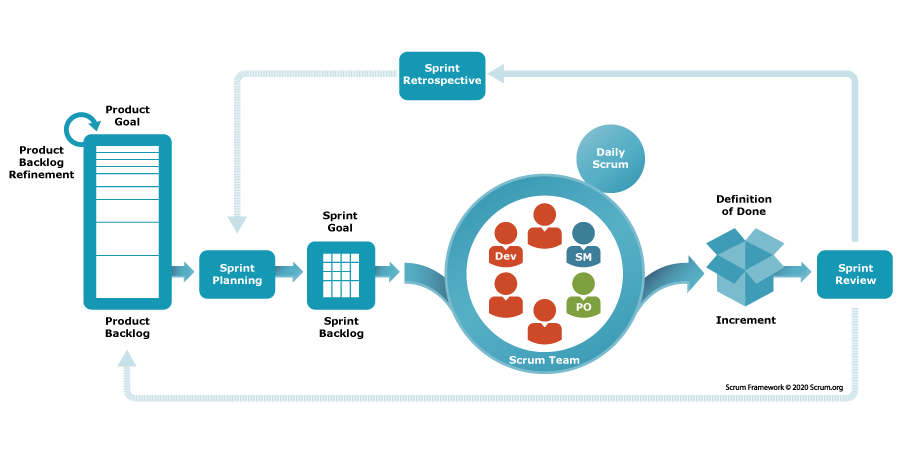
\includegraphics[width=0.9\linewidth]{figures/scrum.png}
    \caption{Schéma du cycle Scrum et de ses principales étapes.}
    \label{fig:scrum_process}
\end{figure}

Les rôles clés définis pour ce projet sont :
\begin{itemize}
    \item \textbf{Product Owner :} Représente les intérêts des utilisateurs finaux et définit les priorités fonctionnelles du backlog.
    \item \textbf{Scrum Master :} Garantit le respect de la méthodologie Scrum, facilite les rituels et élimine les obstacles rencontrés.
    \item \textbf{Équipe de Développement :} Responsable de la réalisation des incréments techniques et de la qualité logicielle.
\end{itemize}

L’équipe Scrum de ce projet est présentée dans le tableau \ref{table:equipe_scrum}.

\begin{table}[H]
\centering
\caption{Équipe Scrum du projet Certif-fun.}
\label{table:equipe_scrum}
\begin{tabular}{|l|l|}
\hline
\textbf{Rôle} & \textbf{Personne en charge} \\ \hline
Product Owner & Pr. LAANAOUI My Driss \\ \hline
Scrum Master & Anas KHAIY \\ \hline
Équipe de Développement & Anas KHAIY \\ \hline
\end{tabular}
\end{table}

\subsection{Planification du projet}
La réalisation de Certif-fun a été structurée en 11 sprints majeurs, permettant une gestion granulaire des complexités techniques de l'IA et des microservices.

\begin{table}[H]
\centering
\caption{Planification détaillée des sprints du projet Certif-fun.}
\label{table:sprints}
\begin{tabular}{|l|p{8cm}|l|}
\hline
\textbf{Sprint} & \textbf{Objectifs et tâches} & \textbf{Livrables} \\ \hline
Sprint 1 & \textbf{Étude préalable et Analyse :} Analyse des besoins, spécifications fonctionnelles et choix de la stack technologique. & Cahier des charges \\ \hline
Sprint 2 & \textbf{Conception (UML et Maquettes) :} Création des diagrammes de cas d'utilisation, de classes et conception des maquettes UI. & Dossier de conception \\ \hline
Sprint 3 & \textbf{Infrastructure Microservices :} Mise en place de l'environnement Docker et des squelettes de services (Spring Boot, FastAPI). & Socle technique \\ \hline
Sprint 4 & \textbf{Réalisation du Frontend (React) :} Création des composants de base, intégration de la charte graphique et mise en place de la navigation. & Interfaces de base \\ \hline
Sprint 5 & \textbf{Sécurité et Authentification :} Développement du système d'authentification centralisé par JWT et gestion des ports (9091-9093). & Module Auth sécurisé \\ \hline
Sprint 6 & \textbf{Gestion des Certifications :} Implémentation des fonctionnalités de gestion des cours et des cycles de certification. & Portails Admin/Formateur \\ \hline
Sprint 7 & \textbf{IA de Proctoring :} Intégration des modèles YOLOv8 et MediaPipe pour la surveillance automatisée en temps réel. & Moteur de surveillance \\ \hline
Sprint 8 & \textbf{Module IA Générative :} Intégration d'Ollama pour la génération automatisée de quiz et de résumés de cours. & Assistant pédagogique IA \\ \hline
Sprint 9 & \textbf{Collaboration et Visioconférence :} Développement de l'espace de réunion virtuelle et communication en temps réel. & Module Visioconférence \\ \hline
Sprint 10 & \textbf{Encadrement et UX :} Système de suivi de progression, filtrage avancé, pagination et optimisation mobile (Responsive). & Interface optimisée \\ \hline
Sprint 11 & \textbf{Tests et Finalisation :} Validation globale, tests de charge, correction des bugs et rédaction du rapport final. & Projet finalisé \\ \hline
\end{tabular}
\end{table}

\subsection{Planification temporelle (Diagramme de Gantt)}
La phase de planification est essentielle dans l'élaboration d'un projet. Elle implique la définition et l'organisation minutieuse des diverses tâches constituant le projet, en évaluant le temps et les ressources requis pour leur accomplissement.

J'ai employé le diagramme de \textbf{Gantt} \cite{ramdani2020ordonnancement}, l'un des outils de planification les plus performants pour illustrer visuellement la progression des diverses tâches qui forment un projet. Dans ce graphique, la colonne de gauche détaille toutes les tâches à réaliser, tandis que la ligne supérieure indique les unités de temps (mois). Chaque tâche est représentée par une barre horizontale dont la position et la longueur représentent la date de début, la durée et la date de fin.

Le projet s'étend du \textbf{15 février au 30 juin}, couvrant l'intégralité du cycle de développement de Certif-fun, comme illustré dans la figure \ref{fig:gantt_certif-fun}.

\begin{figure}[H]
    \centering
    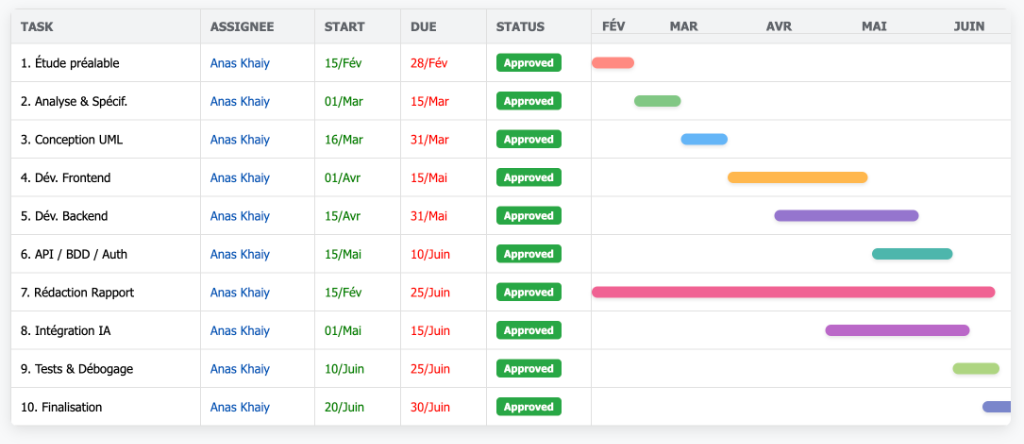
\includegraphics[width=1\linewidth]{figures/gantt_certif-fun.png}
    \caption{Diagramme de Gantt du projet Certif-fun.}
    \label{fig:gantt_certif-fun}
\end{figure}

\section{Conclusion}
En guise de synthèse, ce chapitre a permis de dresser un portrait global du projet \textbf{Certif-fun}. Nous connaissons désormais ses motivations profondes, les insuffisances des solutions actuelles, les objectifs ambitieux à atteindre ainsi que les contraintes techniques et sécuritaires à respecter. Ces éléments permettent de comprendre la pertinence et la finalité de notre travail dans le paysage éducatif actuel.

Malgré une vision claire, certaines difficultés ont été identifiées lors de cette phase initiale, notamment la complexité de l'intégration du traitement vidéo en temps réel au sein d'une architecture microservices et la gestion de la confidentialité des données lors de l'utilisation de modèles d'IA. Ces défis seront abordés avec une attention particulière lors des phases de conception et de réalisation.

Les informations collectées et analysées ici constituent la base solide sur laquelle s'appuiera la suite de notre démarche. Le prochain chapitre détaillera l'\textbf{Étude préliminaire et fonctionnelle}, où nous approfondirons les besoins des utilisateurs, les scénarios métiers et la modélisation des interactions via les diagrammes de cas d'utilisation UML.
 
    \chapter{Étude préliminaire et fonctionnelle}

\section{Introduction}
Ce chapitre a pour objectif de cadrer les besoins auxquels le projet \textbf{CertifEns} doit répondre, qu’ils soient liés aux fonctionnalités principales, aux contraintes techniques ou encore à l’expérience utilisateur. Il permet également de clarifier l’identité des différents acteurs, ainsi que leur rôle dans le système. Enfin, il détaille la logique de fonctionnement au travers de cas d’utilisation et de l’analyse des besoins qui guideront la conception technique.

\section{Étude des besoins}
Dans cette section, nous distinguons deux grandes catégories de besoins : fonctionnels, qui décrivent les services offerts par la plateforme, et non fonctionnels, qui concernent les performances, la fiabilité et la sécurité globale du système.

\subsection{Besoins fonctionnels}
Les besoins fonctionnels représentent les actions spécifiques que le système CertifEns doit être capable d'exécuter pour satisfaire les utilisateurs finaux.

\subsubsection{Liste des fonctionnalités principales}
L'application propose les services essentiels suivants :
\begin{itemize}
    \item \textbf{Gestion des Certifications :} Création et configuration de parcours certifiants avec suivi de progression.
    \item \textbf{Surveillance automatisée (AI Proctoring) :} Détection de fraudes en temps réel via YOLOv8 et analyse du regard avec MediaPipe.
    \item \textbf{Génération de contenu pédagogique par IA :} Création instantanée de quiz et de résumés à l'aide d'Ollama et de modèles LLM locaux.
    \item \textbf{Encadrement et Suivi :} Système de gestion de tâches pour un accompagnement personnalisé des apprenants.
    \item \textbf{Collaboration synchrone :} Module de visioconférence intégré pour les réunions et les sessions de supervision en direct.
\end{itemize}

\subsubsection{Scénarios d'utilisation concrets}
Pour illustrer la valeur ajoutée de CertifEns, voici trois scénarios métiers types impliquant chaque acteur du système :

\begin{enumerate}
    \item \textbf{Scénario Formateur (Productivité et Interaction) :} Le formateur orchestre un cycle de certification depuis son espace dédié. Après avoir automatisé la création des évaluations pédagogiques, il anime des sessions d'échange en direct pour approfondir les concepts avec ses étudiants. Il utilise ensuite les outils de suivi pour assigner des objectifs personnalisés et accompagner la progression de chaque apprenant de manière structurée.
    
    \item \textbf{Scénario Apprenant (Parcours et Réussite) :} L'apprenant suit son évolution via un tableau de bord centralisé. Il participe à des évaluations sécurisées garantissant l'intégrité de son parcours, reçoit des notifications pour ses échéances importantes, et accède en fin de cursus à ses résultats détaillés pour obtenir une certification officielle valorisant ses compétences.
    
    \item \textbf{Scénario Administrateur (Gestion et Gouvernance) :} L'administrateur assure le pilotage global de la plateforme. Il supervise les comptes des différents intervenants, structure l'offre pédagogique en regroupant les formations par thématiques, et analyse les indicateurs de performance globaux pour optimiser la qualité des parcours certifiants proposés par l'organisation.
\end{enumerate}

\subsection{Besoins non fonctionnels}
Ces besoins garantissent que le système fonctionne de manière optimale, sécurisée et évolutive.

\subsubsection{Contraintes de performance, de sécurité et de fiabilité}
\begin{itemize}
    \item \textbf{Performance :} L'analyse vidéo pour le proctoring doit s'effectuer en quasi-temps réel (latence inférieure à 200ms) pour garantir une détection efficace.
    \item \textbf{Sécurité :} L'accès aux portails est protégé par une authentification JWT (\textit{JSON Web Token}). Les données sensibles et les flux vidéo sont sécurisés pour respecter la confidentialité des examens.
    \item \textbf{Fiabilité :} Le système doit assurer une haute disponibilité des services de visioconférence et une persistance sans faille des résultats de certification.
\end{itemize}

\subsubsection{Implications sur le choix de l’architecture et de la technologie}
Ces contraintes de performance et d'intégrité ont dicté nos choix stratégiques :
\begin{itemize}
    \item \textbf{Architecture Microservices :} Adoption d'un découplage entre les services métiers (Admin, Formateur, Apprenant) pour assurer la scalabilité et isoler les briques d'IA très gourmandes en ressources.
    \item \textbf{Frameworks de développement :} 
    \begin{itemize}
        \item \textbf{Spring Boot :} Pour la robustesse des services back-end et la gestion sécurisée des données.
        \item \textbf{FastAPI :} Pour l'exposition haute performance des modèles d'intelligence artificielle en Python.
        \item \textbf{React.js :} Pour une interface utilisateur réactive, moderne et ergonomique.
    \end{itemize}
    \item \textbf{Technologies d'IA et Temps Réel :}
    \begin{itemize}
        \item \textbf{Ollama :} Pour l'exécution locale des modèles de langage (LLM), garantissant la confidentialité des données pédagogiques.
        \item \textbf{LiveKit :} Pour la gestion des flux vidéo et audio haute performance lors des sessions de visioconférence.
        \item \textbf{YOLOv8 et MediaPipe :} Pour une surveillance visuelle (Proctoring) précise et optimisée.
    \end{itemize}
    \item \textbf{Infrastructure et Persistance :}
    \begin{itemize}
        \item \textbf{Docker :} Pour simplifier le déploiement et garantir la cohérence de l'environnement technique à travers toutes les briques de la plateforme.
        \item \textbf{PostgreSQL :} Pour une gestion relationnelle fiable et performante des données de certification.
    \end{itemize}
\end{itemize}

\section{Identification des acteurs}
L'identification des acteurs consiste à définir les différents profils qui interagiront avec le système CertifEns, ainsi que leurs droits et responsabilités respectifs.

\begin{itemize}
    \item \textbf{Administrateur :} Il assure le pilotage global de la plateforme. Ses responsabilités incluent la gestion du cycle de vie des comptes utilisateurs (formateurs et apprenants), l'organisation des formations en cycles et en lots thématiques (\textit{Bundles}), ainsi que la surveillance des indicateurs de performance globaux via des outils d'analyse statistique.
    
    \item \textbf{Formateur :} Acteur central de la pédagogie, il est responsable de la création des contenus et de l'évaluation. Il utilise les outils d'automatisation pour générer des banques de questions, anime les sessions de visioconférence en direct pour le tutorat, et assure un suivi personnalisé via le module d'encadrement structuré. Il a également accès aux rapports de supervision des examens de ses étudiants.
    
    \item \textbf{Apprenant :} Utilisateur final du service d'apprentissage, il accède à son espace personnel pour suivre ses cours et remplir ses objectifs d'encadrement. Il participe aux évaluations surveillées par l'intelligence artificielle et peut, après validation de ses compétences, consulter ses résultats et récupérer ses certificats officiels.
\end{itemize}

\section{Cas d’utilisation et diagrammes}
Les cas d'utilisation (\textit{Use Cases}) permettent de formaliser les interactions entre les acteurs et le système CertifEns. Ils offrent une vision claire des fonctionnalités du point de vue de l'utilisateur final.

\subsection{Présentation des cas d'utilisation}
Chaque acteur interagit avec le système pour atteindre des objectifs spécifiques. Le diagramme de cas d'utilisation global (voir figure \ref{fig:use_case_global}) illustre cette répartition des responsabilités.

\begin{figure}[H]
    \centering
    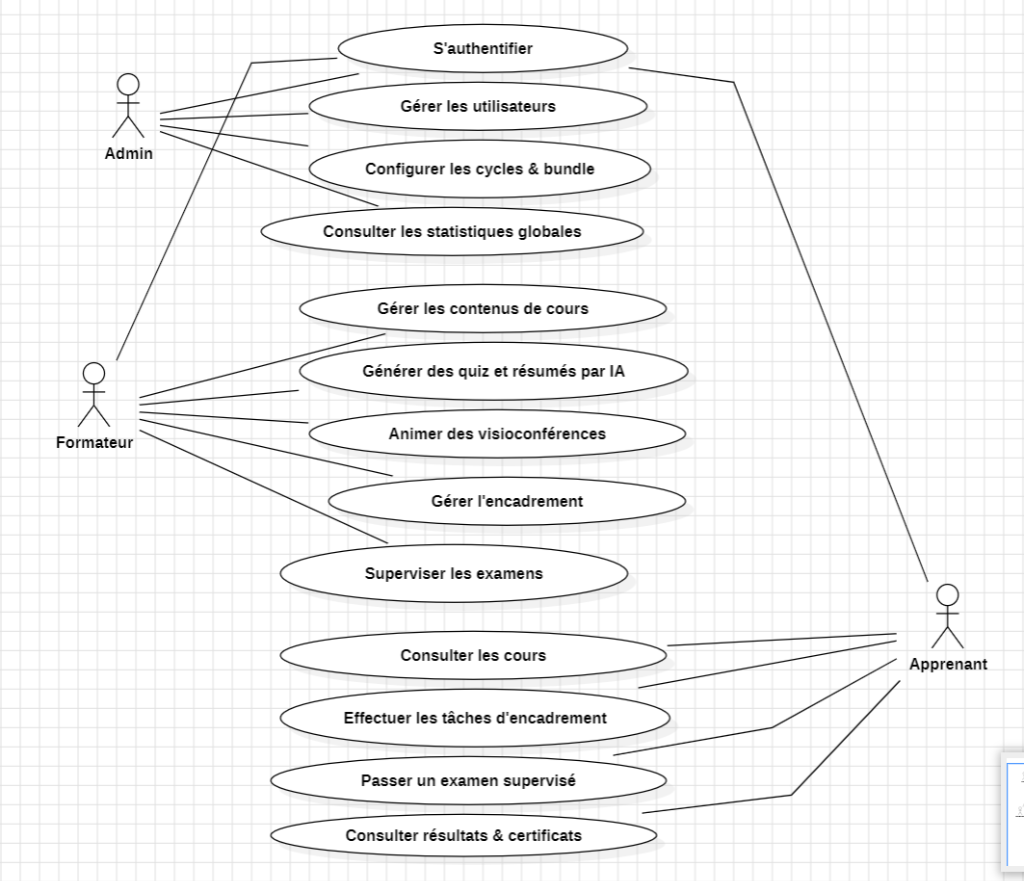
\includegraphics[width=0.85\linewidth]{figures/use_case_global.png}
    \caption{Diagramme de cas d'utilisation global de CertifEns.}
    \label{fig:use_case_global}
\end{figure}

Les cas d'utilisation principaux sont détaillés ci-dessous :
\begin{itemize}
    \item \textbf{Administrateur :}
    \begin{itemize}
        \item \textit{Gérer les utilisateurs :} Création, modification et suppression des comptes formateurs et apprenants.
        \item \textit{Organiser les formations :} Structuration des cours en cycles de certification et en bundles thématiques.
    \end{itemize}
    
    \item \textbf{Formateur :}
    \begin{itemize}
        \item \textit{Générer des évaluations par IA :} Utilisation du moteur LLM pour créer des quiz et des résumés.
        \item \textit{Animer des visioconférences :} Lancement de sessions de tutorat en direct.
        \item \textit{Superviser l'encadrement :} Suivi de la progression des tâches assignées aux apprenants.
    \end{itemize}
    
    \item \textbf{Apprenant :}
    \begin{itemize}
        \item \textit{Passer un examen supervisé :} Réalisation d'une évaluation sous surveillance IA.
        \item \textit{Suivre son parcours :} Consultation du tableau de bord de progression et des tâches d'encadrement.
        \item \textit{Consulter ses certificats :} Accès aux attestations de réussite validées.
    \end{itemize}
\end{itemize}

\subsection{Couverture des besoins fonctionnels}
Cette modélisation assure une couverture complète des besoins identifiés précédemment. Chaque fonctionnalité clé (surveillance, génération de contenu, encadrement) est directement reliée à un cas d'utilisation métier, garantissant ainsi la cohérence et la pertinence du système développé.

\section{Processus métier}
Le processus métier décrit l'enchaînement logique des opérations, depuis la préparation pédagogique jusqu'à la délivrance de la certification. Cette vision dynamique complète la vision statique des cas d'utilisation.

\subsection{Workflow global du système}
Le diagramme de processus présenté en figure \ref{fig:workflow_global} illustre le flux d'informations et les interactions entre les différentes briques technologiques de la plateforme.

\begin{figure}[H]
    \centering
    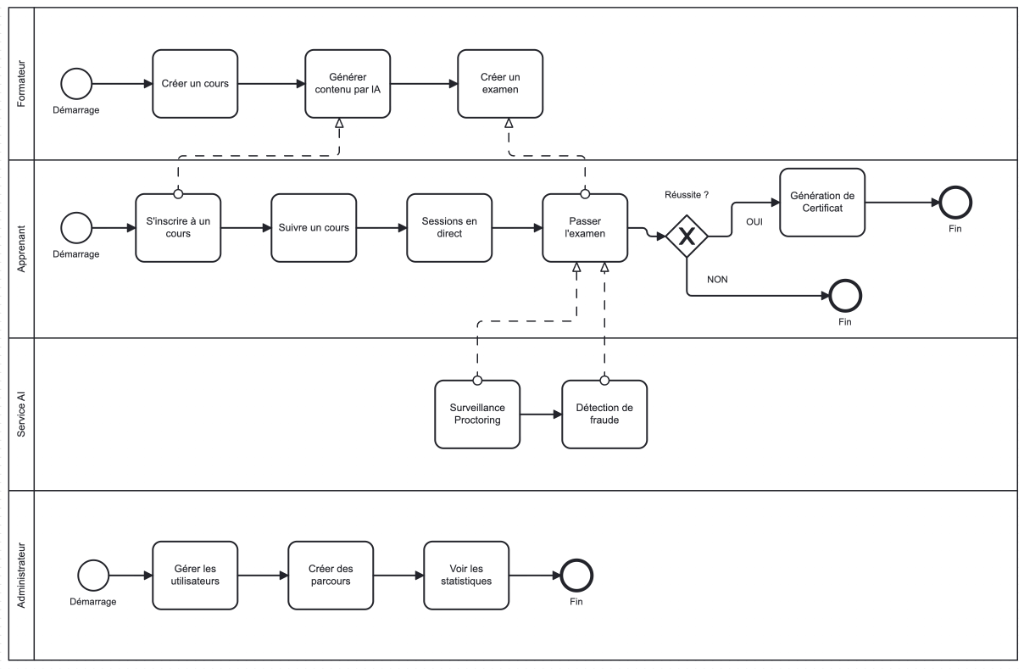
\includegraphics[width=0.85\linewidth]{figures/workflow_global.png}
    \caption{Diagramme de processus métier global (BPMN) de CertifEns.}
    \label{fig:workflow_global}
\end{figure}

\subsection{Validations et étapes-clés}
Le cycle de vie d'une certification repose sur plusieurs jalons critiques :
\begin{enumerate}
    \item \textbf{Gestion Administrative :} L'administrateur prépare l'écosystème en gérant les comptes et en structurant les cycles de formation.
    \item \textbf{Ingénierie Pédagogique :} Le formateur crée les contenus. L'intégration de l'IA permet une validation assistée via la génération de quiz et de résumés.
    \item \textbf{Parcours d'Apprentissage :} L'apprenant suit les modules, participe aux sessions d'échange en direct et effectue ses tâches d'encadrement.
    \item \textbf{Évaluation et Surveillance :} C'est l'étape de contrôle final. Le service de surveillance intelligente analyse les flux en temps réel pour garantir l'intégrité de l'examen. En cas de réussite, le certificat est généré automatiquement. En cas d'échec, le processus prend fin sans délivrance de titre.
\end{enumerate}

\section{Conclusion}
En conclusion, ce chapitre a permis de dresser un bilan synthétique de l'étude fonctionnelle et préliminaire de CertifEns. Nous avons défini une vision claire des fonctionnalités prévues, tout en précisant les rôles et responsabilités de chaque acteur (Administrateur, Formateur, Apprenant). Les contraintes majeures liées à la performance du temps réel et à la sécurité des évaluations ont été identifiées comme des piliers centraux de la conception.

Cette étude pose les bases nécessaires pour la suite de notre démarche. Le chapitre suivant sera consacré à l'\textbf{État de l'art}, où nous confronterons ces besoins avec les solutions et approches technologiques existantes, afin d'affiner la pertinence de nos choix techniques et de positionner CertifEns par rapport aux travaux préexistants dans le domaine de la certification intelligente.

    \chapter{État de l'art}

\section{Introduction}
Le présent chapitre vise à positionner le projet \textbf{Certif-fun} dans son contexte scientifique et technique, en s'appuyant sur un examen des approches et des travaux déjà réalisés dans le domaine. Il a pour rôle de situer notre démarche par rapport aux solutions existantes et d'aider à justifier la pertinence de notre proposition. Nous aborderons ici une recherche bibliographique sur les technologies de surveillance (\textit{Proctoring}), l'IA générative en éducation, ainsi qu'une comparaison des plateformes et architectures actuelles pour mettre en exergue les besoins encore non satisfaits.

\section{Travaux connexes et solutions existantes}
\subsection{Proctoring automatisé (IA de surveillance)}
De nombreux travaux démontrent l'efficacité de systèmes multi-modaux basés sur la vision par ordinateur. Par exemple, \textit{Singh et al.} proposent un proctoring IA qui utilise \textbf{YOLO} pour repérer les objets interdits (téléphones, livres) et \textbf{MediaPipe} pour suivre le visage et les yeux, en traitant en temps réel les flux vidéo des candidats. 

Le système détecte les téléphones et le nombre de personnes via \textbf{YOLOv8}, et peut automatiquement interrompre l'examen lorsqu'une fraude est détectée. D'autres solutions open-source, comme \textit{EduView}, intègrent des modèles TensorFlow et MediaPipe pour l'analyse des mouvements oculaires et utilisent Ultralytics YOLOv8 pour la détection faciale. Ces approches offrent modularité et efficacité sans nécessiter de ressources \textit{cloud}, en signalant en temps réel les activités suspectes.

\subsection{Outils de génération pédagogique par IA}
Plusieurs applications émergentes assistent les enseignants dans la création de quiz. Par exemple, des projets utilisant \textbf{FastAPI} et \textbf{LangChain} illustrent comment exploiter \textbf{Ollama} pour extraire le contenu de documents et générer automatiquement des questionnaires. 

Les recherches académiques corroborent ce potentiel : l'utilisation de grands modèles de langage (\textit{LLM}) peut produire un large éventail de questions alignées sur le cours. Toutefois, les essais montrent souvent une qualité inégale, soulignant que les quiz générés « couvrent un large spectre de sujets » mais peuvent manquer de profondeur dans les domaines de pointe sans un \textit{fine-tuning} approprié ou une supervision humaine.

\subsection{Plateformes existantes}
Certaines plateformes de certification intègrent déjà des fonctions avancées :
\begin{itemize}
    \item \textbf{HackerEarth :} Propose un environnement combinant gestion d'examens, verrouillage du navigateur et analyses anti-plagiat.
    \item \textbf{Moodle :} Le LMS \textit{open-source} s'enrichit désormais de plugins IA. La version 5.0 intègre un fournisseur Ollama permettant d'appeler des modèles LLM locaux pour générer ou résumer des contenus.
    \item \textbf{Solutions propriétaires :} Des outils comme \textit{Proctorio} ou \textit{Respondus} offrent du proctoring automatisé, mais restent fermés et coûteux.
\end{itemize}
Il manque toutefois une solution unifiée liant nativement proctoring et génération de contenu dans un seul système microservices.

\subsection{Architectures et technologies}
Les architectures microservices se démocratisent dans l'EdTech pour répondre aux besoins de scalabilité. Elles offrent un système modulaire où chaque service (gestion utilisateurs, cours, proctoring, visioconférence) est découplé. L'utilisation de \textbf{Spring Boot}, \textbf{FastAPI} et \textbf{React}, associée à \textbf{Docker}, permet une mise à jour isolée de chaque composant et facilite l'intégration d'algorithmes d'IA gourmands en ressources sans impacter le reste de la plateforme.

\section{Analyse comparative}
Cette partie compare les solutions citées selon divers critères techniques, économiques et fonctionnels.

\subsection{Synthèse comparative}
Le tableau \ref{table:comparaison_existant} résume les forces et faiblesses des approches actuelles par rapport à Certif-fun.

\begin{table}[H]
\centering
\caption{Comparaison des solutions existantes avec Certif-fun.}
\label{table:comparaison_existant}
\begin{tabular}{|p{3cm}|p{3cm}|p{3cm}|p{3cm}|}
\hline
\textbf{Critères} & \textbf{LMS Classiques (Moodle)} & \textbf{Proctoring Dédié (Proctorio)} & \textbf{Certif-fun} \\ \hline
\textbf{Surveillance IA} & Via plugins tiers & Très avancée & \textbf{Native (YOLOv8)} \\ \hline
\textbf{Génération IA} & Limitée / Externe & Aucune & \textbf{Native (Ollama)} \\ \hline
\textbf{Architecture} & Monolithique & Propriétaire & \textbf{Microservices} \\ \hline
\textbf{Coût} & Gratuit (Open source) & Élevé (Licence) & \textbf{Open Source / Local} \\ \hline
\textbf{Collaboration} & Basique & Absente & \textbf{Visioconférence intégrée} \\ \hline
\end{tabular}
\end{table}

\subsection{Analyse des aspects stratégiques}
\begin{itemize}
    \item \textbf{Aspects techniques :} L'association YOLOv8 + MediaPipe permet un traitement en temps réel sur du matériel standard, surpassant les versions antérieures en rapidité.
    \item \textbf{Aspects économiques :} L'usage d'Ollama (LLM local) réduit les coûts d'API cloud (OpenAI) et préserve la confidentialité des données (RGPD).
    \item \textbf{Aspects fonctionnels :} Certif-fun se distingue en unifiant sécurité et pédagogie, là où les autres solutions sont spécialisées dans un seul domaine.
\end{itemize}

\section{Conclusion}
Pour conclure ce chapitre, il est essentiel de faire une mise en perspective. L'analyse de l'état de l'art a permis de constater que si des solutions performantes existent pour la surveillance d'examens ou la gestion de cours, elles restent souvent incomplètes ou perfectibles car elles ne proposent pas d'intégration native et unifiée de l'intelligence artificielle générative et de la surveillance intelligente au sein d'une même architecture modulaire.

Cette étude de l'existant confirme et oriente nos choix stratégiques : l'adoption d'une architecture microservices pour la scalabilité, ainsi que l'utilisation de modèles locaux (\textit{Edge IA}) pour garantir à la fois performance et confidentialité des données. Les conclusions tirées ici serviront de base solide pour élaborer, dans le chapitre suivant, une architecture adaptée et une modélisation \textbf{UML} rigoureuse. Ce cadrage des approches préexistantes met en relief la valeur ajoutée de Certif-fun et pave la voie à la phase de \textbf{Conception} technique de notre solution.

    \chapter{Analyse et conception}
\label{ch:analysis_design}

% =============================
% INTRODUCTION
% =============================
\section{Introduction}
L'objectif de ce chapitre est de traduire les besoins fonctionnels et non fonctionnels, identifiés lors de la phase d'analyse, en une solution technique détaillée et structurée. Cette étape de conception est cruciale car elle permet de définir l'ossature du système avant l'implémentation. Nous détaillerons ici les choix architecturaux, le formalisme de modélisation adopté ainsi que les diagrammes UML qui décrivent tant la structure statique que le comportement dynamique de Certif-fun. Ces choix sont justifiés par la nécessité de répondre aux exigences de scalabilité, de performance en temps réel et de sécurité propres à une plateforme de certification intelligente.

\section{Formalisme de modélisation : UML}
\subsection{Motivation et choix}
UML (\textit{Unified Modeling Language}) est un langage visuel standardisé pour modéliser un système logiciel. Il offre un ensemble de diagrammes (classes, cas d’utilisation, séquence, etc.) permettant de représenter précisément l’architecture, le comportement et les interactions complexes du système \cite{deshmukh2023uml}.

\begin{figure}[H]
    \centering
    
\includegraphics[width=0.2\linewidth]{figures/UML_logo.png}
    \caption{Logo du formalisme UML utilisé pour la modélisation.}
    \label{fig:uml_logo}
\end{figure}

L'utilisation de ce formalisme pour Certif-fun répond à plusieurs objectifs :
\begin{itemize}
    \item Description de la structure et du comportement : UML permet de visualiser le système sous plusieurs angles (statique avec les classes, dynamique avec les séquences).
    \item Communication efficace : Il sert de langage commun entre les intervenants du projet pour lever toute ambiguïté sur les flux de données.
    \item Garantie de cohérence et maintenabilité : Une conception rigoureuse facilite l'évolution future du code et identifie les incohérences logiques.
\end{itemize}

\subsection{Diagrammes retenus}
Dans le cadre de ce projet, nous avons retenu les diagrammes suivants pour formaliser notre conception :
\begin{itemize}
    \item Diagramme de classes : Pour représenter la structure statique des entités (Utilisateurs, Cours, Certificats) et leurs relations.
    \item Diagrammes de séquence : Pour illustrer les interactions complexes entre les microservices (ex: processus de surveillance Proctoring).
    \item Diagramme de déploiement : Pour visualiser l'organisation physique des composants (conteneurs Docker, bases de données) sur l'infrastructure.
\end{itemize}

% =============================
% ARCHITECTURE LOGICIELLE
% =============================
\section{Architecture logicielle}
Cette section décrit l’architecture globale du système, en distinguant clairement l’approche adoptée et en expliquant la répartition fonctionnelle et technique du code.

\subsection{Approche architecturale}
Pour le projet Certif-fun, nous avons confronté deux approches majeures : l'architecture monolithique et l'architecture microservices.

\begin{itemize}
    \item \textbf{Architecture monolithique :} Il s'agit d'une architecture traditionnelle où toutes les fonctionnalités d’une application sont réunies dans un seul programme. Tous les composants sont interdépendants et exécutés dans un même processus \cite{elgheriani2022differential}. Bien qu'elle offre une simplicité initiale, elle présente des inconvénients majeurs en termes de maintenance et de scalabilité ; dans notre cas, la charge de l'IA ralentirait l'ensemble de la plateforme.
    
    \item \textbf{Architecture microservices :} C'est une architecture qui divise une application en petits services autonomes pouvant être développés, déployés et mis à l’échelle indépendamment. Chaque service remplit une fonction métier spécifique et communique via des API bien définies \cite{bozic2023microservices}. Ce choix s'est imposé comme une évidence pour Certif-fun, offrant une scalabilité fine (pour le service IA), une isolation des pannes et une flexibilité technologique (Java/Spring Boot pour le métier et Python/FastAPI pour l'IA).
\end{itemize}

\subsection{Schéma de l'architecture et organisation en couches}
L'architecture de Certif-fun est conçue selon un modèle multicouche qui favorise la séparation des préoccupations et la modularité. Le schéma suivant illustre l'organisation globale du système :

\begin{figure}[H]
    \centering
    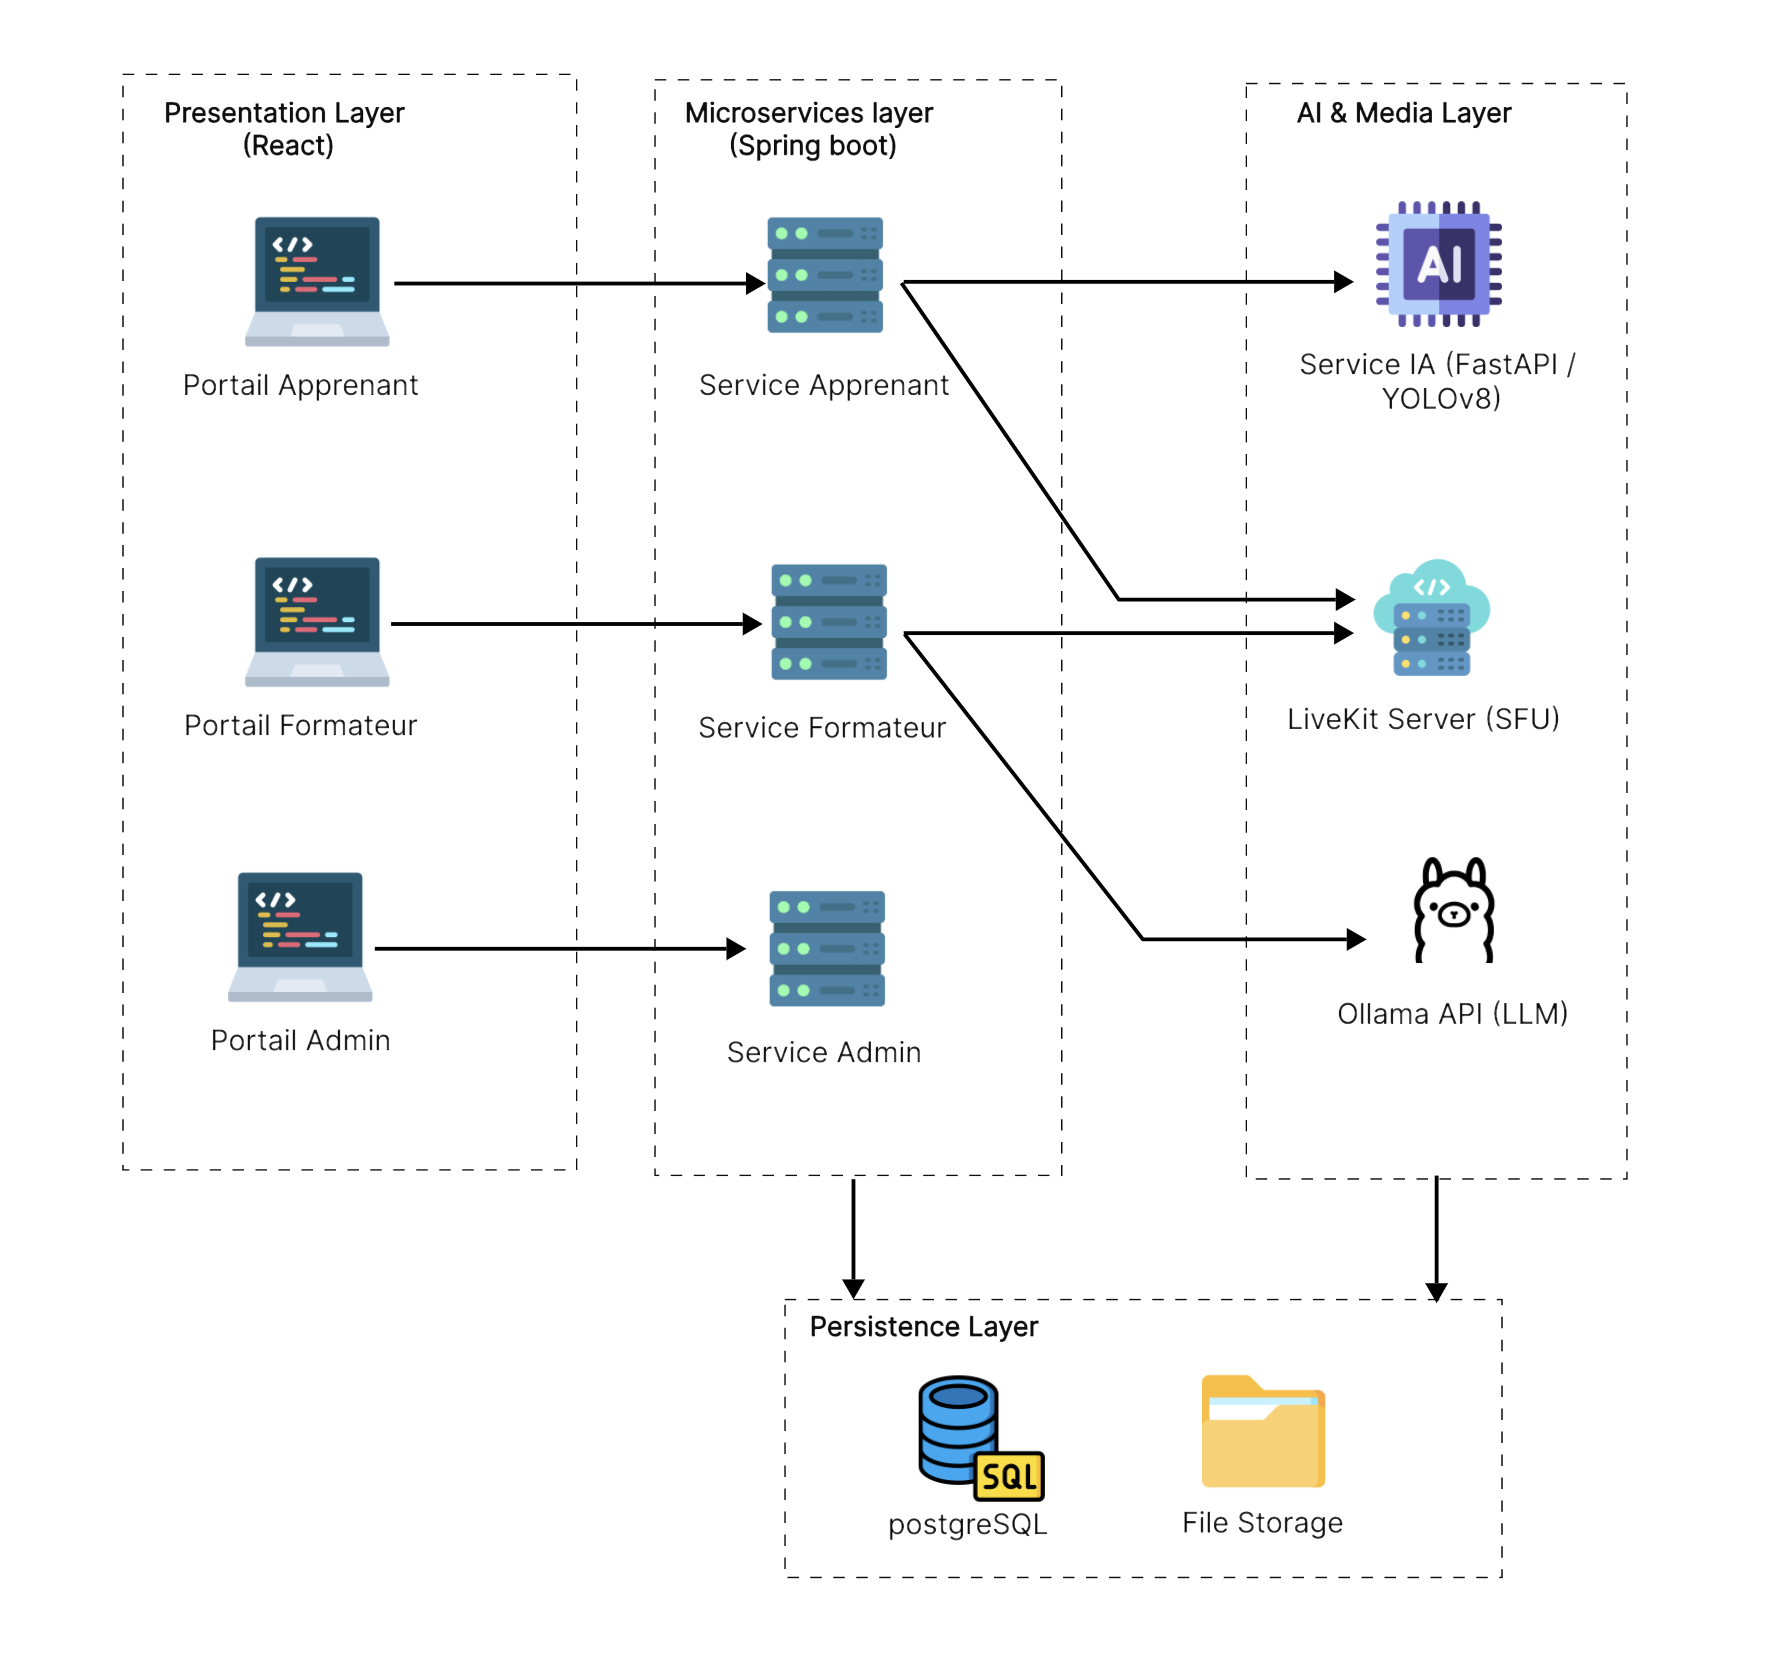
\includegraphics[width=1\linewidth]{figures/architecture_globale.png}
    \caption{Schéma de l'architecture globale du système Certif-fun.}
    \label{fig:architecture_globale}
\end{figure}

Comme illustré dans le diagramme ci-dessus, le système s'articule autour de quatre couches majeures :
\begin{itemize}
    \item Presentation Layer (React) : Regroupe les trois portails web (Apprenant, Formateur, Admin) qui servent d'interface utilisateur unique pour chaque profil.
    \item Microservices Layer (Spring Boot) : Constitue le cœur métier du système. Chaque service gère un domaine spécifique (Utilisateurs, Cours, Encadrement) et communique de manière isolée.
    \item AI \& Media Layer : Cette couche spécialisée gère les traitements lourds. Elle inclut le service de surveillance IA (FastAPI/YOLOv8), la visioconférence (LiveKit SFU) et la génération de contenu (Ollama LLM).
    \item Persistence Layer : Assure la conservation des données via PostgreSQL et le stockage des fichiers numériques (vidéos, ressources).
\end{itemize}

\subsection{Discussion}
Cette architecture répond aux besoins stratégiques du projet :
\begin{itemize}
    \item Maintenabilité : Le découpage permet de modifier un service (ex: mettre à jour le modèle IA) sans impacter les portails d'administration.
    \item Scalabilité : Face à une session d'examen massive, nous pouvons multiplier les instances du microservice de surveillance sans surcharger les autres services.
    \item Sécurité : L'utilisation de tokens JWT entre les couches garantit que les communications sont sécurisées et que les droits d'accès sont strictement respectés.
\end{itemize}

% =============================
% DIAGRAMMES DE CONCEPTION
% =============================
\section{Diagrammes de conception}
Cette section détaille les différents diagrammes qui ont servi à formaliser la conception du système.

\subsection{Diagramme de classes}
Le diagramme de classes est un diagramme UML structurel qui représente l'architecture statique d'un système orienté objet. Il est couramment utilisé pour modéliser les concepts, les données et les entités logiques du système \cite{miro_class_diagram}. Le diagramme suivant présente cette structure pour le système Certif-fun, détaillant les entités, leurs attributs ainsi que les relations qui les unissent.

\begin{figure}[H]
    \centering
    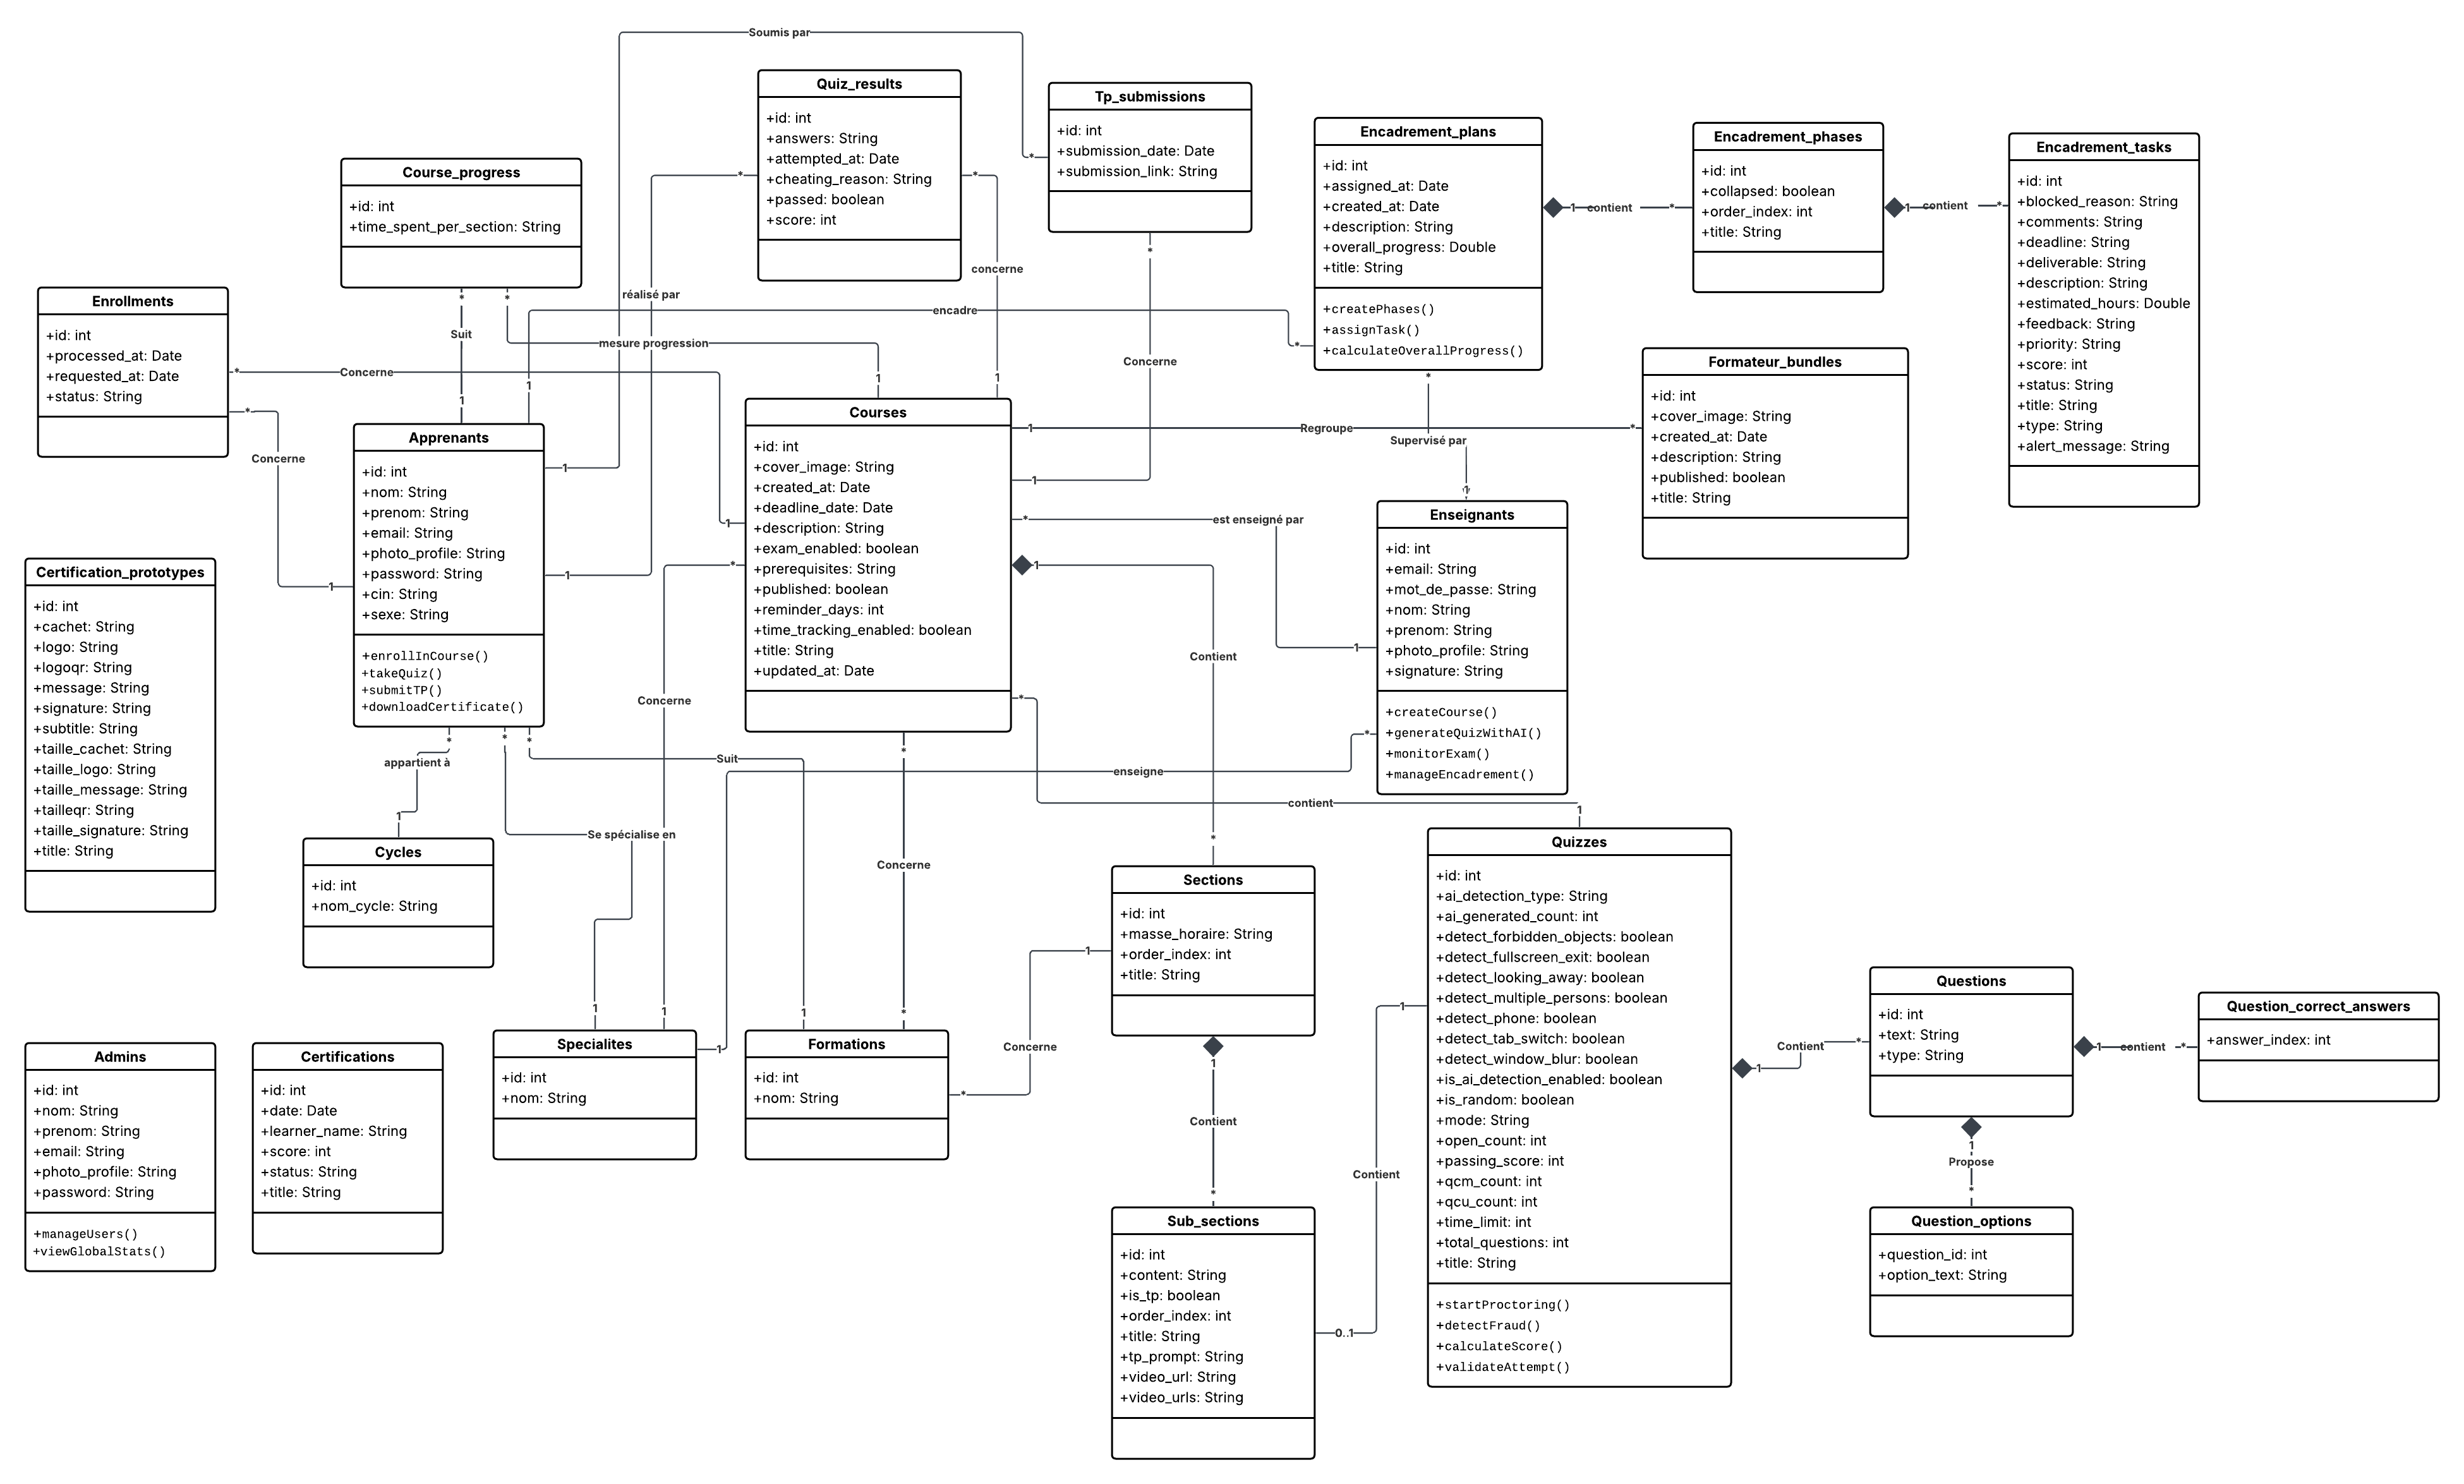
\includegraphics[width=1\linewidth]{figures/diagramme_classes.png}
    \caption{Diagramme de classes global de la base de données certif\_db.}
    \label{fig:diagramme_classes}
\end{figure}

\subsection{Analyse détaillée des entités et de leurs rôles métier}
Cette section détaille les responsabilités de chaque entité au sein de l'écosystème Certif-fun.

\paragraph{A. Gestion des Acteurs et de la Sécurité}
\begin{itemize}
    \item Classe Apprenant : C'est l'acteur central du système. Son rôle est de consommer le contenu pédagogique et de réaliser les examens finaux.
    \item Classe Enseignant (Formateur) : Il agit en tant qu'architecte pédagogique et mentor, concevant les parcours et assurant le suivi.
\end{itemize}

\paragraph{B. Structure Pédagogique et Contenu}
\begin{itemize}
    \item Classe Course (Cours) : Unité d'enseignement pivot entre les formateurs et les apprenants.
    \item Classe Section \& SubSection : Permettent un découpage logique et progressif du savoir (vidéo, texte, quiz).
    \item Classe FormateurBundle : Permet de créer des parcours thématiques regroupant plusieurs cours.
\end{itemize}

\paragraph{C. Évaluation Intelligente (IA \& Proctoring)}
\begin{itemize}
    \item Classe Quiz : Définit le cadre de l'examen final et porte les règles de surveillance IA (fraude, temps limite).
    \item Classe QuizResult : Conserve la trace de la performance et des alertes générées par l'IA.
\end{itemize}

\paragraph{D. Module d'Encadrement de Projet}
\begin{itemize}
    \item Classe EncadrementPlan : Structure la relation de tutorat et définit les objectifs du projet.
    \item Classe EncadrementTask : Représente une action concrète à réaliser (livrables et feedbacks).
\end{itemize}

\paragraph{E. Certification et Persistance}
\begin{itemize}
    \item Classe Certification : Aboutissement du processus attestant officiellement de la réussite.
    \item Classe CertificationPrototype : Gère l'aspect visuel, la mise en page et le format de signature.
\end{itemize}

\subsection{Diagrammes de séquence}
Le diagramme de séquence est un diagramme UML comportemental d'interaction qui montre comment les différents objets ou acteurs d'un système coopèrent en échangeant des messages au fil du temps \cite{miro_sequence_diagram}. Les diagrammes suivants illustrent cette dynamique pour Certif-fun.

\subsubsection{Passage d'examen avec surveillance IA (Proctoring)}
Ce diagramme détaille le flux de surveillance en temps réel. Pendant que l'apprenant répond aux questions, son flux vidéo est analysé par YOLOv8 pour détecter toute fraude (téléphone, absence) et alerter immédiatement le backend.

\begin{figure}[H]
    \centering
    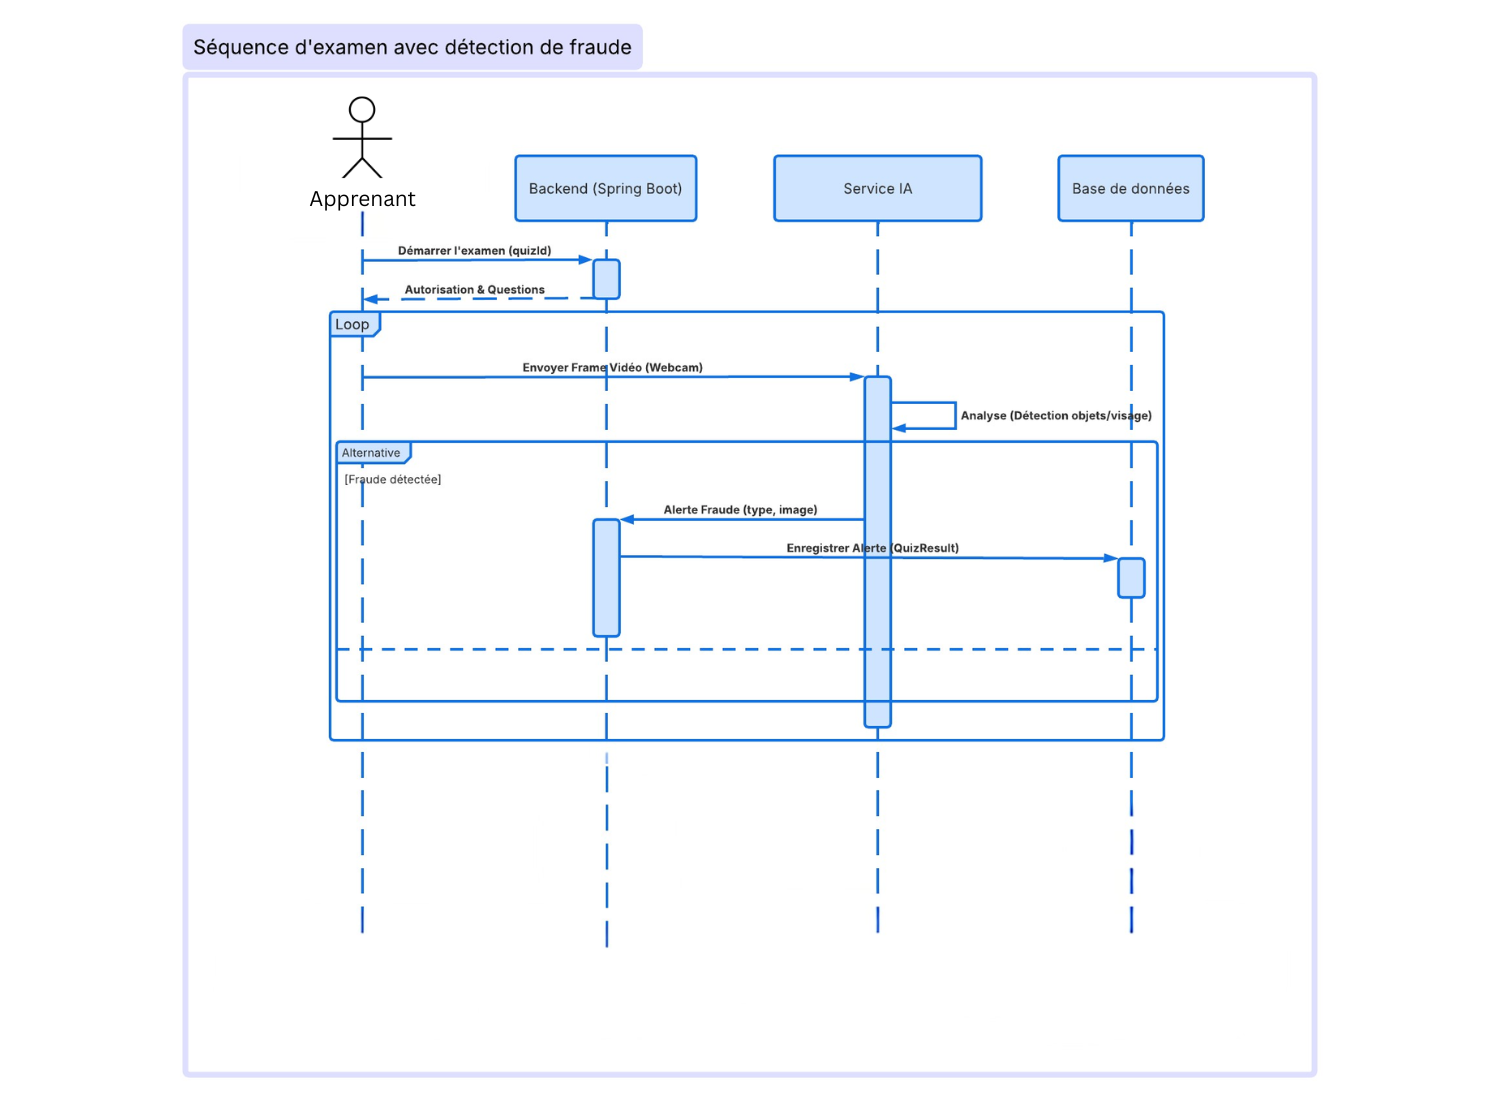
\includegraphics[width=0.9\linewidth]{figures/sequence1.png}
    \caption{Diagramme de séquence du processus de surveillance IA.}
    \label{fig:seq_proctoring}
\end{figure}

\subsubsection{Processus d'Encadrement et d'Évaluation}
Ce scénario illustre le cycle allant de la création d'une tâche d'encadrement à la soumission du livrable et au feedback du formateur, assurant un suivi pédagogique rigoureux.

\begin{figure}[H]
    \centering
    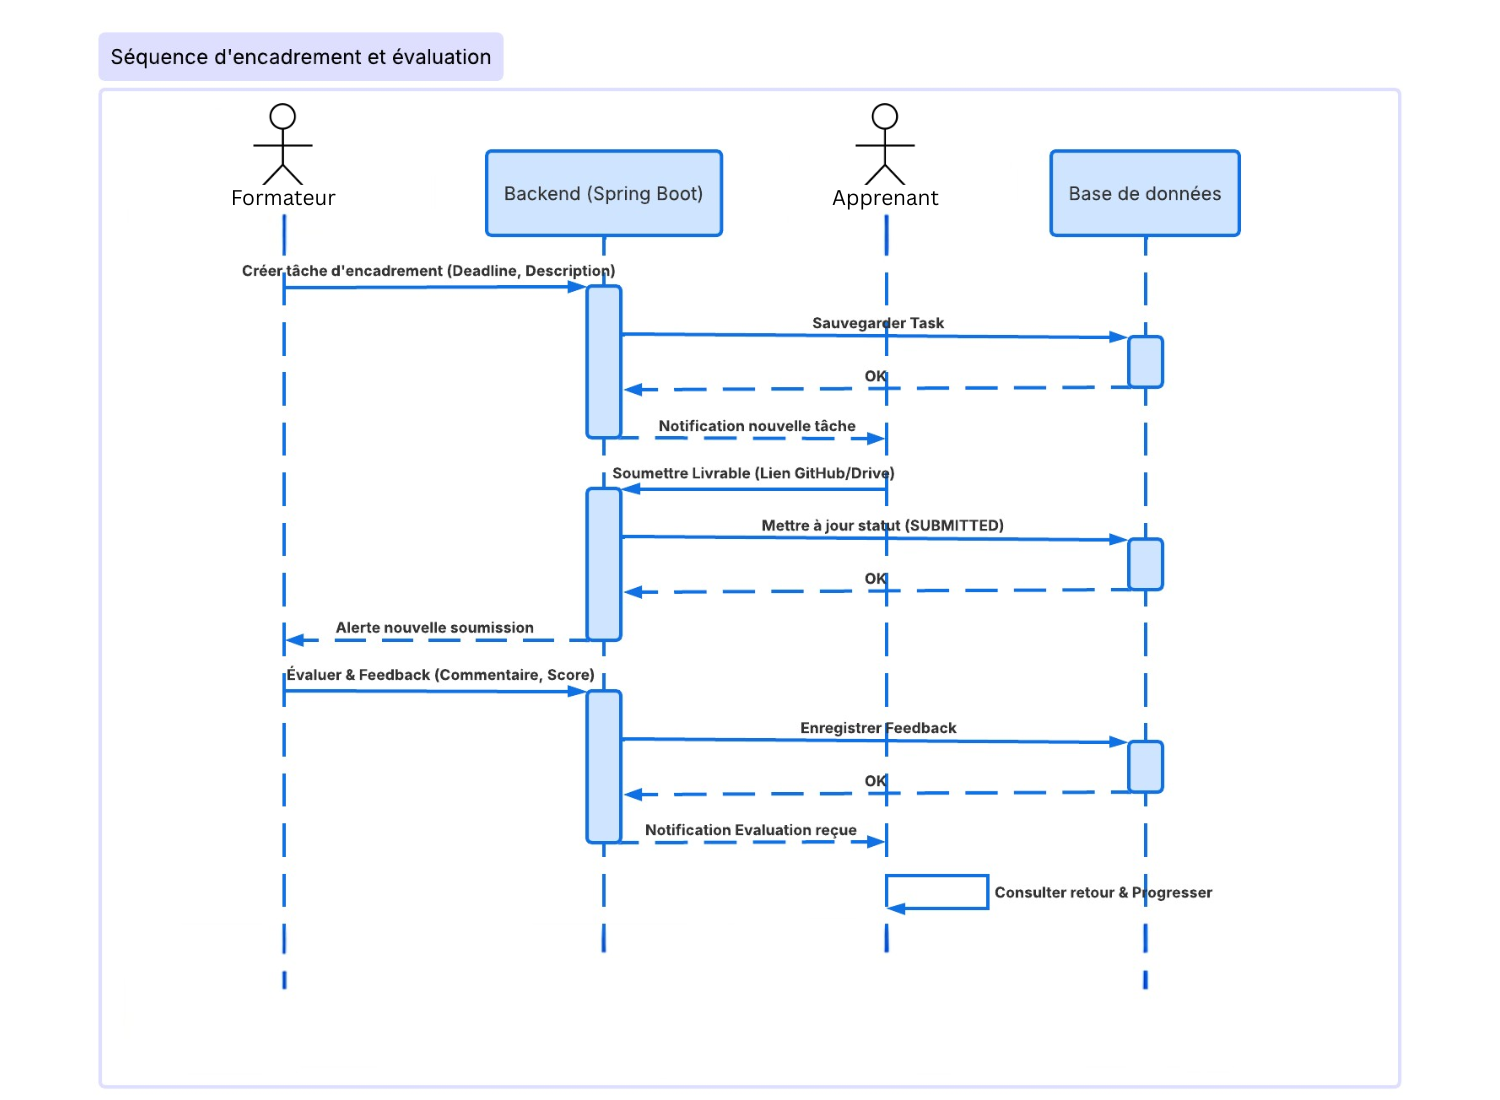
\includegraphics[width=0.9\linewidth]{figures/sequence2.png}
    \caption{Diagramme de séquence de l'encadrement et de l'évaluation.}
    \label{fig:seq_encadrement}
\end{figure}

\subsubsection{Génération de Quiz assistée par LLM (Ollama)}
Ce diagramme montre comment le backend prépare un prompt structuré pour Ollama afin de générer un quiz JSON prêt à être publié par l'enseignant.

\begin{figure}[H]
    \centering
    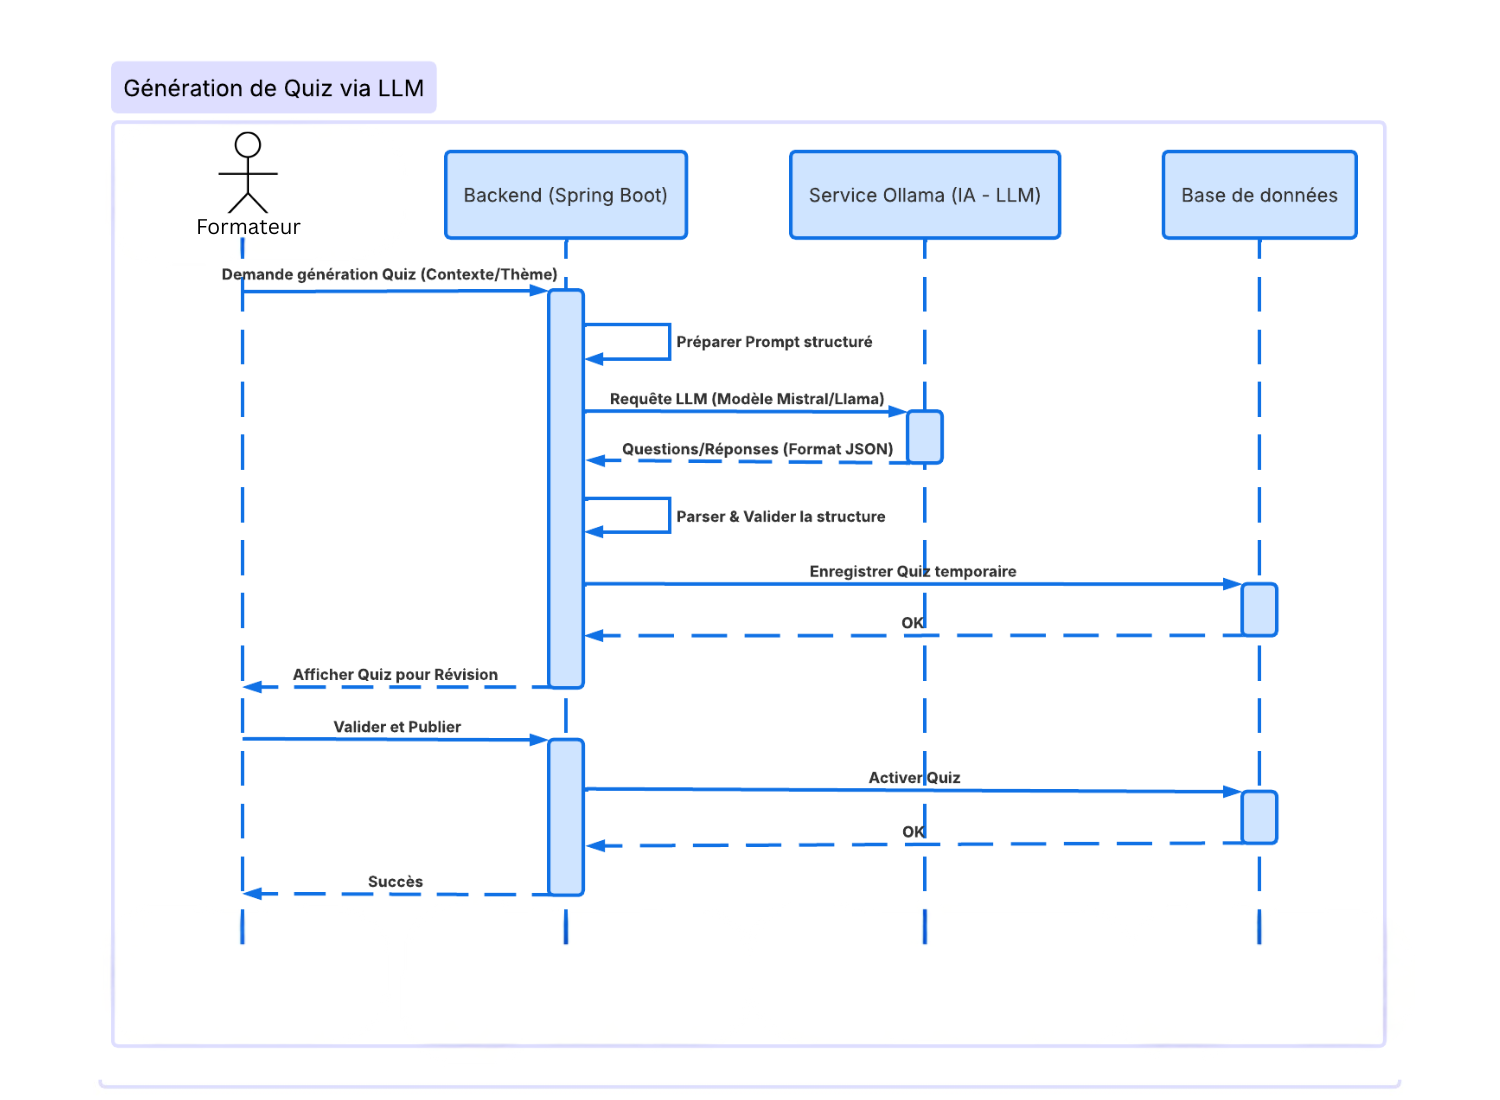
\includegraphics[width=0.9\linewidth]{figures/sequence3.png}
    \caption{Diagramme de séquence de la génération de quiz par LLM.}
    \label{fig:seq_ollama}
\end{figure}

\subsubsection{Visioconférence et Collaboration via LiveKit}
Ce scénario décrit la négociation WebRTC facilitée par le serveur LiveKit (SFU), assurant une distribution fluide et scalable des flux médias entre participants.

\begin{figure}[H]
    \centering
    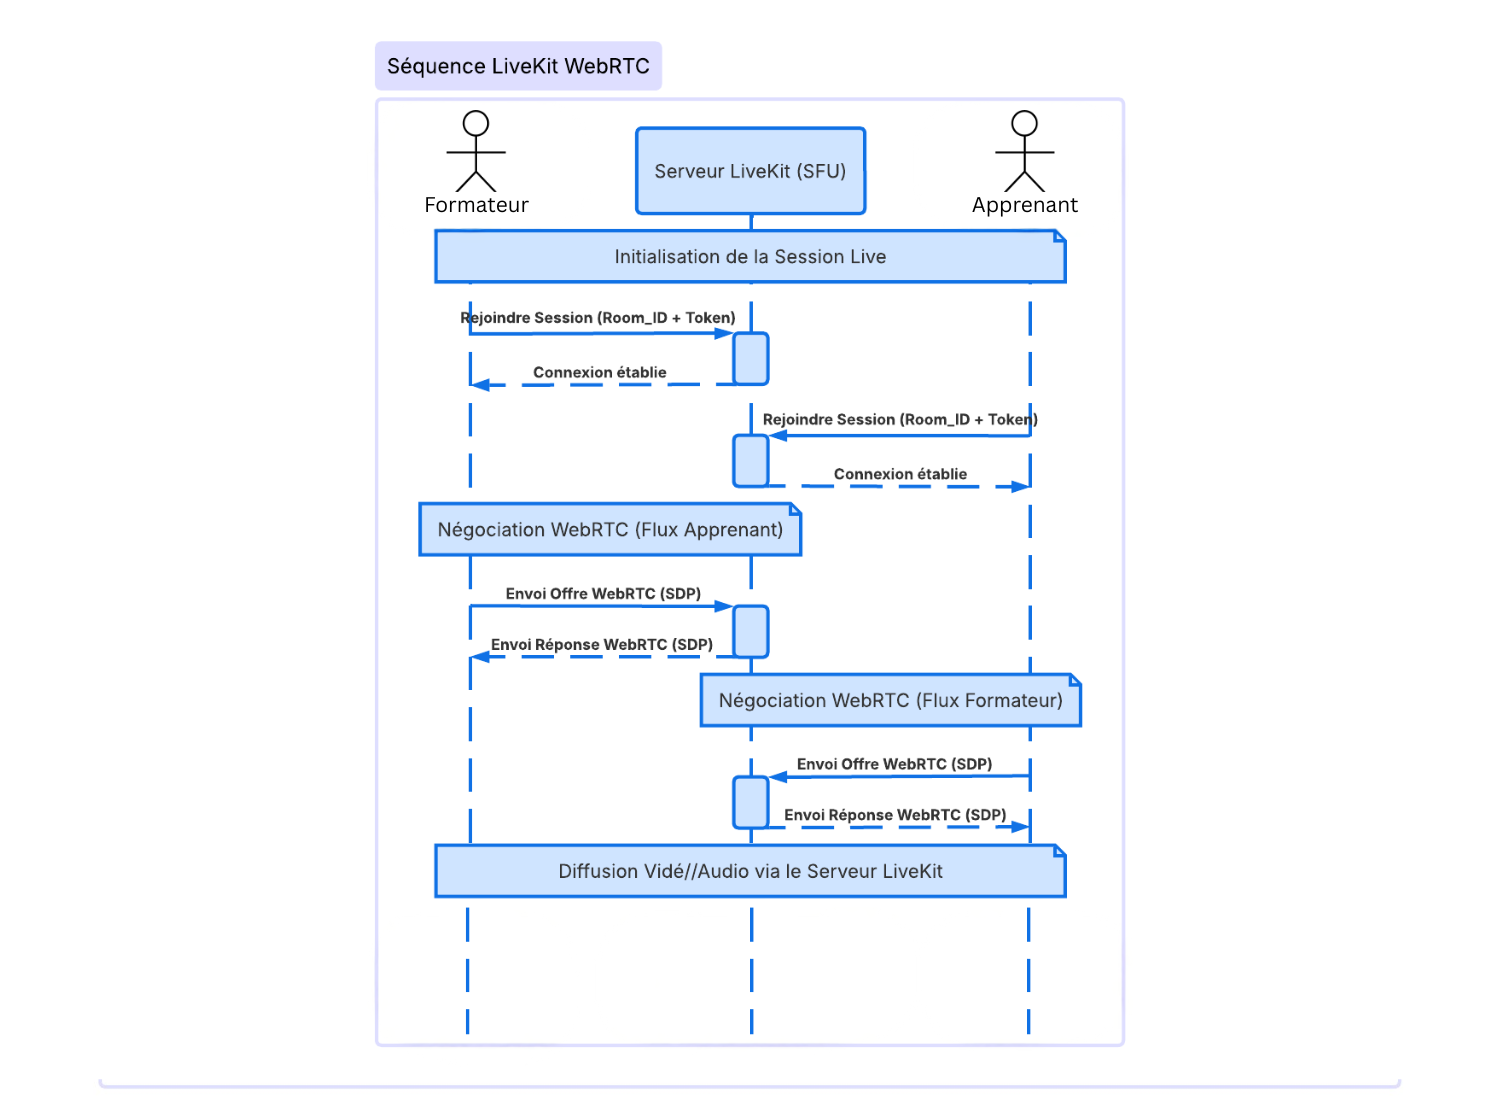
\includegraphics[width=0.85\linewidth]{figures/sequence4.png}
    \caption{Diagramme de séquence de la visioconférence WebRTC.}
    \label{fig:seq_livekit}
\end{figure}

\subsubsection{Authentification et Accès à l'Examen}
Ce diagramme détaille les quatre phases critiques du module de vérification d'identité : le scan du code QR pour la validation de l'inscription, la vérification de l'authenticité du document (carte d'étudiant), la reconnaissance faciale biométrique et enfin l'autorisation d'accès à l'examen.

\begin{figure}[H]
    \centering
    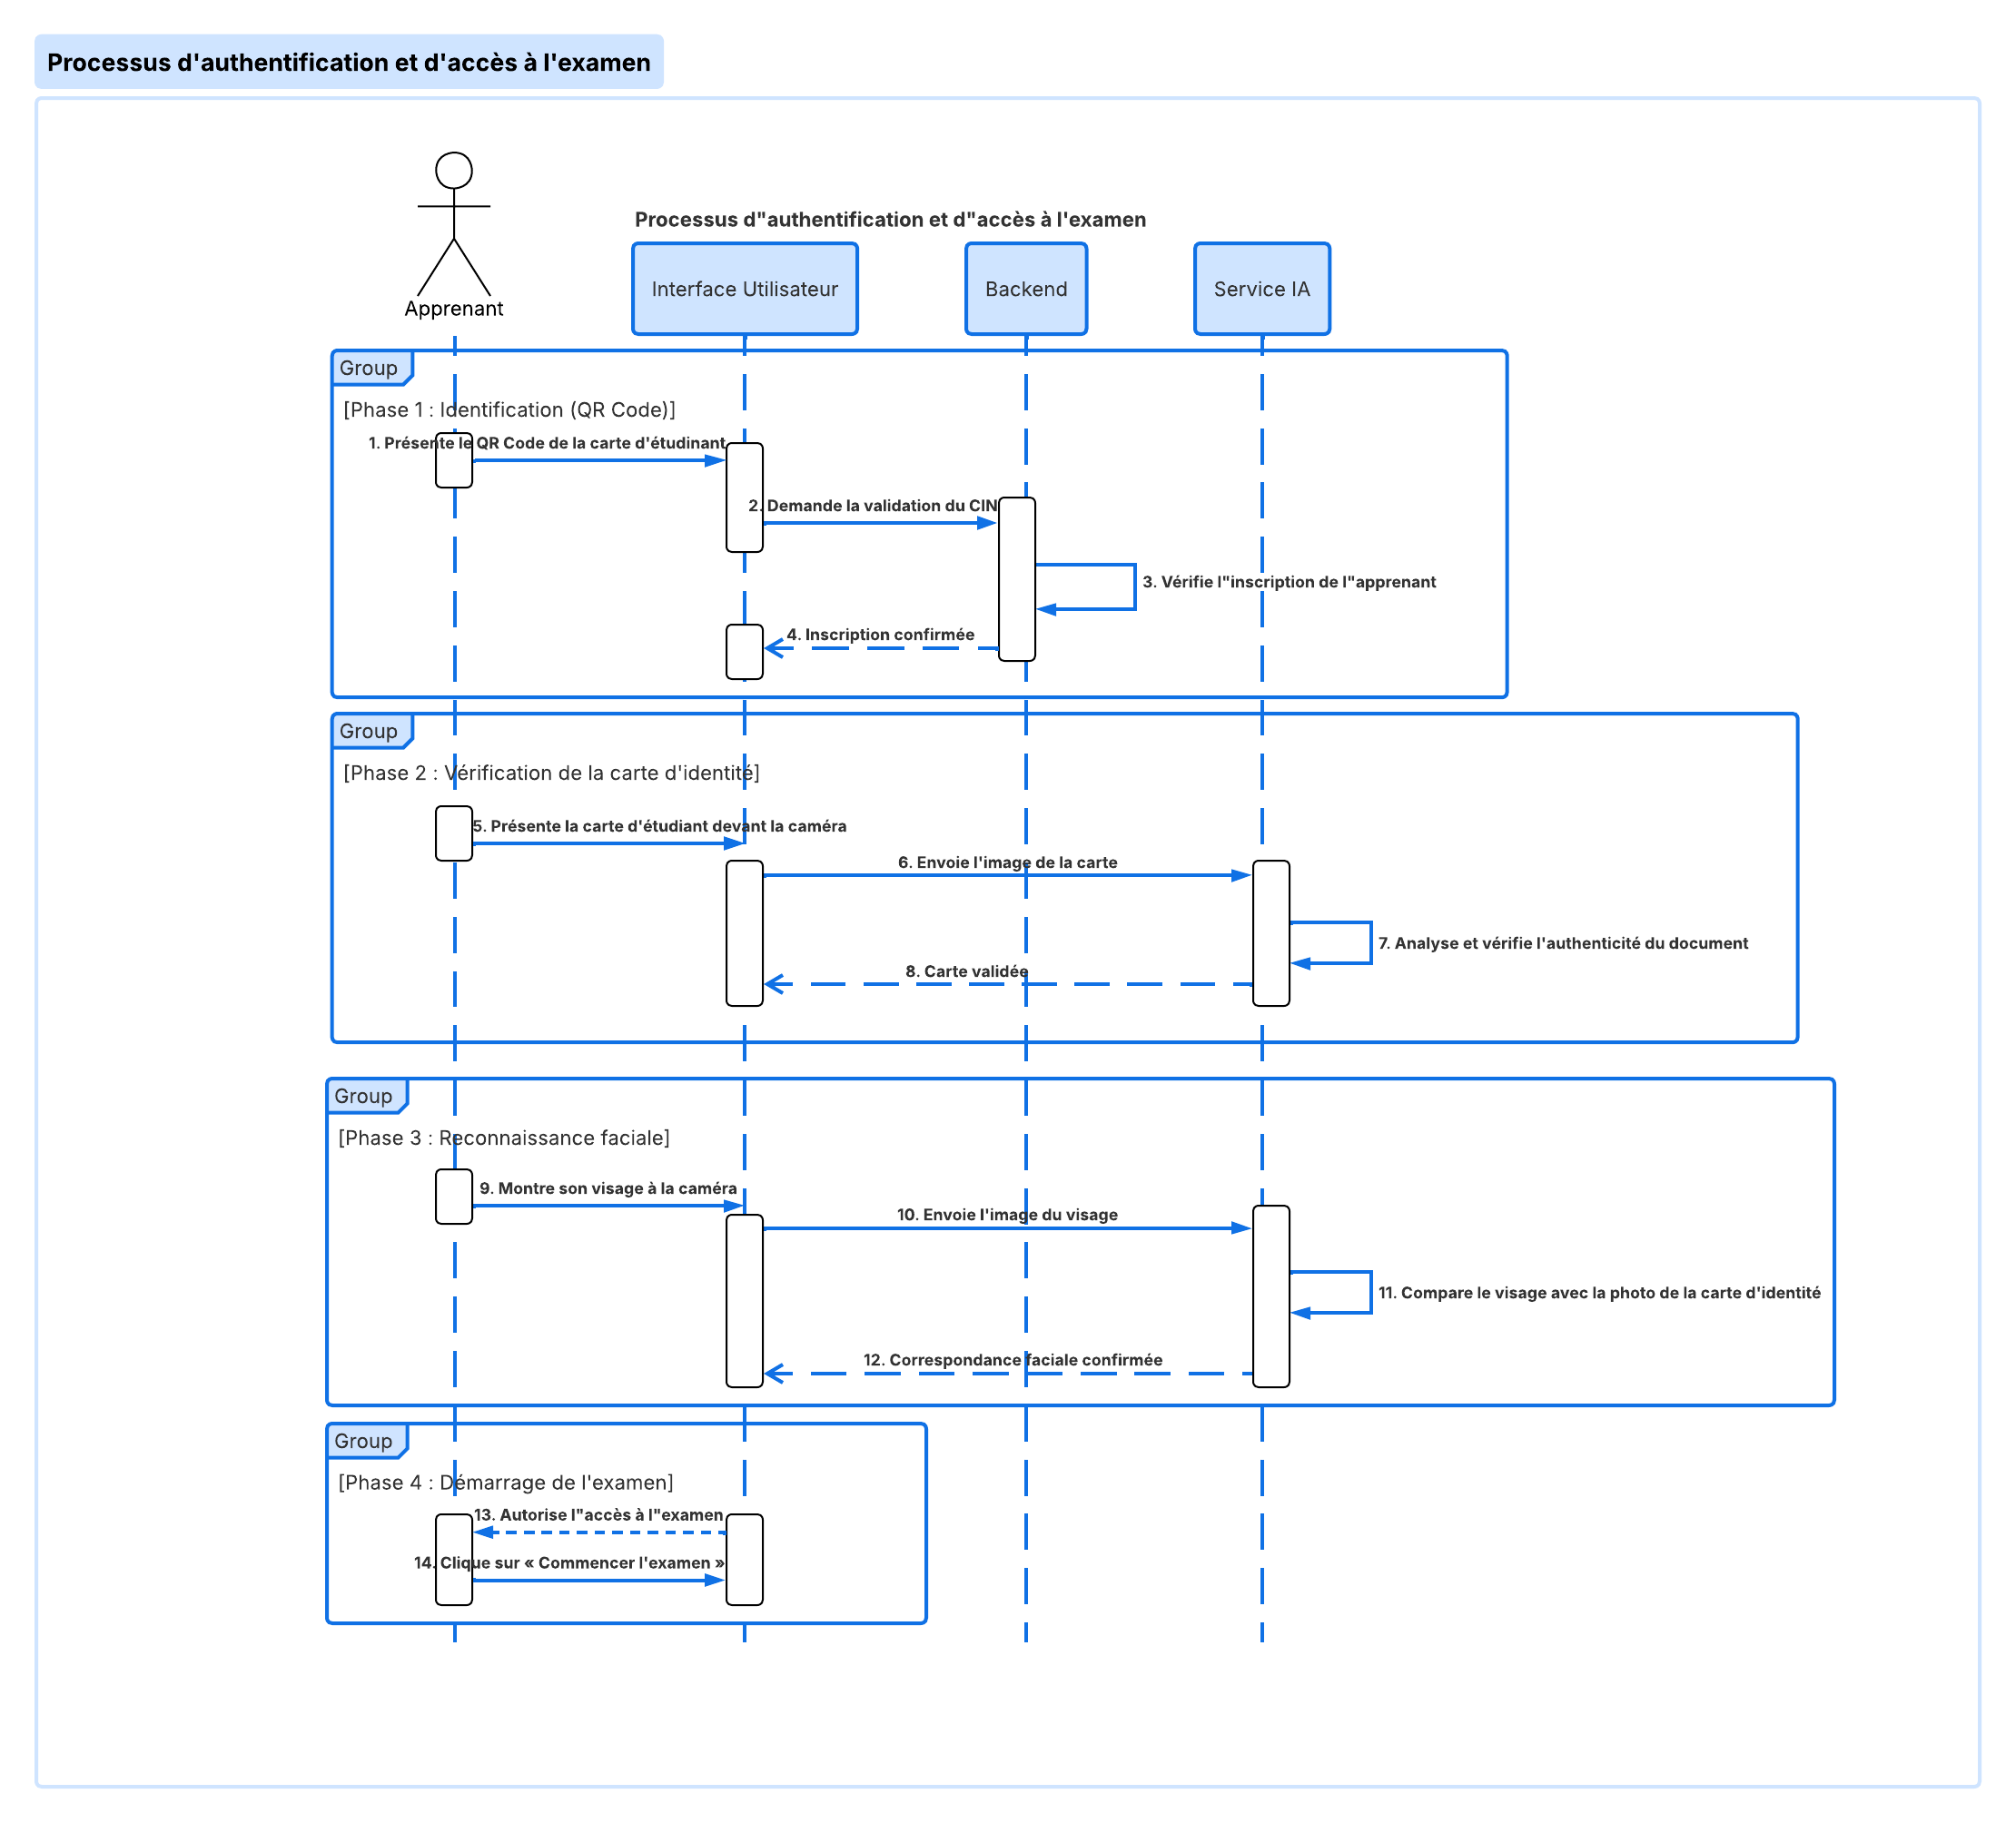
\includegraphics[width=0.98\linewidth]{figures/sequence5.png}
    \caption{Diagramme de séquence du processus d'authentification et d'accès à l'examen.}
    \label{fig:seq_auth_examen}
\end{figure}

\section{Conclusion}
En conclusion, ce chapitre a permis de poser les fondements techniques de la plateforme Certif-fun à travers une modélisation rigoureuse et une architecture microservices parfaitement adaptée aux enjeux du projet. Le choix du formalisme UML pour les diagrammes de classes et de séquences, combiné à une architecture découpée en couches fonctionnelles, garantit une séparation nette des responsabilités entre les modules. Cette structure facilite non seulement l'intégration de services complexes tels que la surveillance proactive par IA et la visioconférence en temps réel, mais elle simplifie également la maintenance et les évolutions futures du système. Ces décisions architecturales assurent une modularité optimale et répondent aux exigences critiques de performance, de haute disponibilité et de sécurité, indispensables à une plateforme de certification de ce calibre. Les modèles et schémas ainsi définis constituent le socle technique indispensable sur lequel s'appuiera la phase de réalisation pratique et de déploiement, dont les détails techniques et les interfaces seront présentés de manière approfondie dans le chapitre suivant.

    \chapter{Technologies et réalisation}

Ce chapitre décrit l'ensemble des technologies, outils et méthodes qui ont été utilisés pour la mise en œuvre du projet. Il présente d'abord les choix techniques, puis détaille l'environnement de déploiement, l'implémentation du système (structure du code et interfaces utilisateur), ainsi que la stratégie de tests appliquée. Enfin, une conclusion synthétique fait le point sur les réalisations et les éventuelles difficultés rencontrées.

%%%%%%%%%%%%%%%%%%%%%%%%%%%%%%%%%%%%%%%%%%%%%%%%%%%%%%%%%%%
\section{Introduction}
%%%%%%%%%%%%%%%%%%%%%%%%%%%%%%%%%%%%%%%%%%%%%%%%%%%%%%%%%%%
Dans cette section introductive, l'objectif est de donner une vue d'ensemble des aspects techniques et pratiques abordés dans ce chapitre. Nous y expliquons notamment :
\begin{itemize}
    \item \textbf{Les choix technologiques :} Justification des outils et frameworks sélectionnés en fonction des besoins fonctionnels (scalabilité, sécurité) et des contraintes techniques du projet.
    \item \textbf{L'environnement de déploiement :} La manière dont l'infrastructure est configurée, notamment via la conteneurisation, pour supporter l'écosystème microservices.
    \item \textbf{L'implémentation et l'interface utilisateur :} Les détails sur la structuration du code source (backend et frontend) et la conception ergonomique des interfaces.
    \item \textbf{La stratégie de validation :} La méthodologie adoptée pour tester le système et garantir sa conformité aux exigences initiales.
\end{itemize}

Cette partie prépare le lecteur à comprendre comment les décisions prises au niveau de la conception se traduisent concrètement lors de la réalisation technique de la plateforme Certif-fun.

%%%%%%%%%%%%%%%%%%%%%%%%%%%%%%%%%%%%%%%%%%%%%%%%%%%%%%%%%%%
\section{Choix techniques et outils}
%%%%%%%%%%%%%%%%%%%%%%%%%%%%%%%%%%%%%%%%%%%%%%%%%%%%%%%%%%%
La sélection de la pile technologique pour \textbf{Certif-fun} n'est pas fortuite ; elle résulte d'une analyse comparative visant à concilier réactivité, sécurité et modularité.

\subsection{Langages, Frameworks et Bases de données}
Cette sous-section détaille l'ensemble des piliers technologiques et outils d'infrastructure sur lesquels repose l'ossature de la plateforme \textbf{Certif-fun} :

\begin{itemize}
    \item \textbf{Framework Backend (Java/Spring Boot) :}  
    Spring Boot a été choisi pour orchestrer la coordination entre nos différents microservices (Admin, Formateur, Apprenant) grâce à sa configuration simplifiée \cite{bairstow2023spring}. Son architecture basée sur l’Inversion de Contrôle (IoC) assure un couplage faible entre les modules, facilitant grandement la maintenance du système. Pour la sécurité, nous avons intégré Spring Security afin de gérer rigoureusement l’authentification via des jetons JWT.
    
    \item \textbf{Framework Frontend (React \& Tailwind CSS) :}  
    React permet de construire des interfaces utilisateur interactives basées sur des composants réutilisables et une gestion efficace du Virtual DOM \cite{minnick2022foundation}. Ce choix est indispensable pour rafraîchir les vues instantanément et afficher en temps réel les alertes de surveillance ou les indicateurs de session. Nous l’avons associé à Tailwind CSS dont l’approche utilitaire offre une grande liberté pour concevoir une interface moderne et adaptable.
    
    \item \textbf{Intelligence Artificielle (Python/FastAPI \& YOLOv8) :}  
    YOLOv8 assure la détection d’objets en temps réel pour identifier l’utilisation de téléphones ou la présence de plusieurs personnes \cite{sohan2025review}. FastAPI expose ces capacités via des API hautes performances, facilitant la validation automatique des données et la génération de documentation \cite{fastapi_docs}. Enfin, MediaPipe est intégré pour construire des pipelines de perception multimédia dédiés au suivi précis des visages et des poses \cite{lugaresi2019mediapipe}.
    
    \item \textbf{Visioconférence (LiveKit \& WebRTC) :}  
    Nous utilisons les normes WebRTC pour permettre une communication audio et vidéo fluide directement dans le navigateur sans nécessiter de plugins \cite{romano2012webrtc}. LiveKit s’appuie sur une architecture SFU (Selective Forwarding Unit) qui transfère la charge du routage des flux médias vers le serveur. Cette approche garantit une stabilité optimale tout en allégeant significativement la consommation CPU du navigateur des apprenants.
    
    \item \textbf{Grands Modèles de Langage (Ollama / Mistral, Llama \& Qwen) :}  
    Ollama facilite le déploiement local des modèles de langage tels que Mistral 7B et Llama 3.2 pour la génération automatique de quiz \cite{novais2025using}. Ce choix délibéré garantit la confidentialité totale des données pédagogiques car aucune information ne transite vers des API externes. Le système produit des réponses structurées en JSON qui sont directement intégrées et exploitées par notre application.
    
    \item \textbf{Orchestration et Conteneurisation (Docker \& Docker Compose) :}  
    L’ensemble des composants de la plateforme a été encapsulé dans des conteneurs Docker pour garantir une cohérence parfaite entre les environnements \cite{ibrahim2021docker}. Docker Compose nous permet de démarrer toute l’infrastructure en une seule commande tout en isolant le réseau interne des services. Cette organisation simplifie le déploiement et assure la portabilité de la solution sur différents serveurs.
    
    \item \textbf{Routage et Proxy Inverse (Nginx) :}
    Nginx joue le rôle de point d’entrée unique pour rediriger efficacement les requêtes vers les services frontends et backends appropriés \cite{reese2008nginx}. Il optimise les performances globales de la plateforme grâce à la compression des ressources et à la distribution intelligente de la charge. En outre, il renforce la sécurité en gérant les règles CORS et en ajustant les limites de taille des requêtes HTTP.
    
    \item \textbf{Gestion de Versions et Collaboration (Git \& GitHub) :}  
    Git a constitué un outil incontournable pour garder une trace précise de l’évolution du code source de chacun de nos microservices. L'hébergement sur GitHub a permis de structurer le développement de façon méthodique grâce à un flux de travail collaboratif efficace. Cette organisation a également facilité la mise en place d'un processus de déploiement plus fluide et mieux contrôlé.
    
    \item \textbf{Persistance des données (PostgreSQL) :}  
    PostgreSQL a été retenu pour sa fiabilité et sa conformité aux propriétés ACID, garantissant l’intégrité des données lors de transactions complexes \cite{google_postgresql}. Nous utilisons Spring Data JPA couplé à Hibernate pour offrir un mapping objet-relationnel performant et sécurisé entre le code et la base de données. Ce choix permet de stocker et d'interroger efficacement l'ensemble des données structurées liées aux certifications.
\end{itemize}

\subsection{Outils de développement et collaboration}
La qualité du code, la rigueur de la modélisation et la fluidité globale du cycle de développement ont été assurées par une sélection rigoureuse d'outils professionnels :

\begin{itemize}
    \item \textbf{Environnements de Développement (IDE) :}  
    Nous avons tiré parti de la complémentarité entre deux éditeurs majeurs pour optimiser notre productivité. VS Code a été utilisé pour le Frontend et la partie IA grâce à sa légèreté et ses extensions spécialisées. IntelliJ IDEA a été réservé au développement des microservices Java pour son support natif exceptionnel de Spring Boot.
    
    \item \textbf{Gestion de Versions et Dépôts (Git \& GitHub) :}  
    Git a été au cœur de la gestion du code source avec une stratégie de branches par fonctionnalité pour un travail parallèle sécurisé. Le dépôt privé sur GitHub a assuré une synchronisation fiable et une sauvegarde continue du projet. Cette organisation a permis de structurer le développement de façon méthodique tout au long du cycle de vie.
    
    \item \textbf{Gestionnaires de Dépendances et de Build (Maven \& NPM/Vite) :}  
    La gestion des dépendances a été segmentée selon la nature des couches applicatives du système. Maven s’est chargé de la compilation et du cycle de vie des microservices Spring Boot. Pour la partie Frontend, nous avons combiné la puissance de NPM pour les paquets et la rapidité de Vite pour le build.
    
    \item \textbf{Serveur d'automatisation (Jenkins) :}
    Jenkins est utilisé comme serveur d’automatisation open-source pour piloter nos pipelines CI/CD \cite{jenkins2015continuous}. Il automatise les étapes critiques de compilation, de test et de génération des artifacts de déploiement. Cette approche garantit une livraison continue stable et réduit les risques d'erreurs humaines.
    
    \item \textbf{Frameworks de Test (JUnit 5 \& pytest) :}
    JUnit 5 est employé pour l'écriture et l'exécution des tests unitaires automatisés au sein de l'écosystème Java \cite{kleuker2019junit5}. Parallèlement, pytest simplifie la validation du code Python dédié aux modules d'intelligence artificielle \cite{pytest_docs}. Cette double couverture assure une robustesse logicielle sur l'ensemble des microservices du projet.
    
    \item \textbf{Tests et Validation d'APIs (Postman \& Newman) :}
    Postman a servi d'interface principale pour le développement et le test unitaire des points de terminaison REST. Newman permet d'automatiser l'exécution de ces collections de tests directement en ligne de commande \cite{postman_newman_docs}. Cette combinaison facilite la validation rigoureuse des échanges de données entre le frontend et le backend.
    
    \item \textbf{Administration de Bases de données (pgAdmin 4) :}  
    pgAdmin 4 a été utilisé comme interface graphique principale pour interagir avec nos bases de données PostgreSQL. Il nous a permis d'inspecter les schémas générés par Hibernate et d'exécuter des scripts SQL de débogage. Cet outil a été essentiel pour surveiller l'intégrité des données tout au long de la phase de réalisation.
    
    \item \textbf{Contrôle et Exécution des LLMs (Ollama CLI) :}  
    La gestion des modèles de langage a été pilotée directement depuis le terminal via l'interface en ligne de commande d'Ollama. Cet outil a permis de configurer les modèles Mistral et Llama 3.2 tout en testant leurs comportements via des invites personnalisées. Il assure une intégration fluide des capacités génératives au sein de notre service de quiz.
    
    \item \textbf{Modélisation et Conception UML (StarUML, Draw.io \& Lucidchart) :}  
    StarUML a été l'outil de référence pour produire les diagrammes structurels et comportementaux conformes aux standards. Draw.io et Lucidchart ont complété cette phase pour l'élaboration de schémas d'architecture plus souples et accessibles. Ces outils ont garantit une documentation technique claire et structurée pour l'ensemble du système.
\end{itemize}

\subsection{Protocoles et bibliothèques de support}
En complément des frameworks majeurs, plusieurs protocoles et bibliothèques spécialisées ont été intégrés pour assurer la fluidité des échanges et la robustesse des fonctionnalités :

\begin{itemize}
    \item \textbf{Communication REST et JSON :} 
    L'intégralité des échanges de données entre les frontends React et les microservices Spring Boot repose sur des API REST. Le format JSON a été privilégié pour sa légèreté et sa compatibilité native avec JavaScript, facilitant le mapping des données complexes.
    
    \item \textbf{Sécurisation via JWT (JSON Web Tokens) :} 
    Pour garantir une architecture \textit{stateless} et sécurisée, nous avons implémenté l'authentification par jetons JWT \cite{mahindrakar2020jwt}. Ce protocole permet de transporter les informations d'identité et les rôles utilisateur de manière cryptée, évitant ainsi le stockage de sessions sur le serveur et facilitant la scalabilité des microservices.
    
    \item \textbf{Axios (Client HTTP) :} 
    Côté frontend, la bibliothèque \textbf{Axios} a été utilisée pour orchestrer les appels asynchrones vers les backends. Elle nous a permis de mettre en place des intercepteurs pour injecter automatiquement le token JWT dans les en-têtes de chaque requête et de gérer de manière centralisée les erreurs HTTP.
    
    \item \textbf{Spring Data JPA et Hibernate :} 
    Pour la couche de persistance, nous avons utilisé Spring Data JPA couplé à Hibernate. Cette approche permet de manipuler les données PostgreSQL sous forme d'objets Java, automatisant ainsi la génération des schémas et garantissant l'intégrité référentielle des données.
    
    \item \textbf{MediaPipe et OpenCV :} 
    Pour le module de proctoring, nous avons couplé YOLOv8 avec les bibliothèques \textbf{MediaPipe} \cite{lugaresi2019mediapipe} et \textbf{OpenCV}. MediaPipe assure le suivi des points de repère faciaux (Landmarks) pour l'analyse du regard, tandis qu'OpenCV gère les flux d'images et les transformations matricielles nécessaires avant l'inférence.
\end{itemize}

%%%%%%%%%%%%%%%%%%%%%%%%%%%%%%%%%%%%%%%%%%%%%%%%%%%%%%%%%%%

\begin{itemize}
    \item \textbf{Processeur (CPU) :} 4 cœurs vCPU virtuels (architecture x86\_64), garantissant un traitement parallèle efficace des requêtes REST, de l'inférence YOLOv8 et de la génération de texte par les modèles de langage.
    \item \textbf{Mémoire Vive (RAM) :} 16 Go de RAM DDR4 ECC, une capacité indispensable pour faire tourner simultanément les trois instances Java/Spring Boot, le serveur d'IA Ollama et la base de données PostgreSQL, sans risquer de saturation mémoire (Out of Memory).
    \item \textbf{Stockage Disque :} 200 Go en NVMe SSD, offrant des vitesses de lecture/écriture élevées, essentielles pour le chargement rapide des modèles YOLOv8, le stockage persistant des cours et quiz, ainsi que la réactivité des index PostgreSQL.
    \item \textbf{Bande Passante Réseau :} 16 To de trafic mensuel sur un port réseau à 1 Gbps, suffisant pour supporter les flux de visioconférence WebRTC via LiveKit SFU et le téléchargement des médias de cours par plusieurs apprenants en simultané.
    \item \textbf{Système d'Exploitation (OS) :} Linux Ubuntu Server 24.04 LTS, retenu pour sa stabilité, sa compatibilité avec l'écosystème Docker et son niveau de sécurité éprouvé.
    \item \textbf{Moteur de Conteneurisation :} Docker version 29.5.0 et Docker Compose v5.1.3, assurant le déploiement unifié et l'orchestration de l'ensemble des services de la plateforme.
\end{itemize}

\subsection{Stratégie de conteneurisation via Docker et Docker Compose}
Pour s'affranchir du problème classique de divergence entre les environnements de développement et de production, l'intégralité de la plateforme Certif-fun a été conteneurisée avec Docker. Cette approche de virtualisation légère au niveau du noyau garantit que chaque composant s'exécute dans un environnement rigoureusement identique, quel que soit le système hôte sous-jacent.

L'orchestration de l'ensemble des conteneurs est assurée par Docker Compose v5.1.3, à travers un fichier de configuration central \path{docker-compose.yml} qui structure trois aspects essentiels du déploiement :

\begin{itemize}
    \item \textbf{Isolation réseau :} Tous les conteneurs communiquent au sein d'un réseau privé virtuel de type Bridge, que nous avons nommé \texttt{certif-net}. Seuls Nginx et LiveKit exposent des ports accessibles depuis l'extérieur, ce qui empêche tout accès direct non autorisé à des services sensibles comme PostgreSQL ou Ollama.
    \item \textbf{Persistance des données :} Nous avons pris soin de mettre en place des volumes nommés Docker (\texttt{postgres\_data} et \texttt{ollama\_data}) pour dissocier les données du cycle de vie des conteneurs. Ainsi, même lors d'une mise à jour ou d'un redémarrage complet du serveur, les données utilisateurs, les certifications et les modèles d'IA préalablement téléchargés demeurent intacts.
    \item \textbf{Gestion de l'ordre de démarrage :} La directive \texttt{depends\_on} nous a permis de définir un ordre logique d'initialisation des services, en veillant notamment à ce que PostgreSQL et Ollama soient pleinement opérationnels avant le lancement des microservices Java et Python.
\end{itemize}

\subsection{Topologie et distribution des conteneurs applicatifs}
Le déploiement de la plateforme \textbf{Certif-fun} sur le serveur VPS s'organise autour d'une architecture conteneurisée comprenant onze conteneurs autonomes orchestrés par Docker Compose. Cette répartition permet d'isoler les responsabilités et de garantir la robustesse du système :

\begin{enumerate}
    \item \textbf{Portails Frontends (3 conteneurs) :} 
    Trois conteneurs distincts hébergent les interfaces utilisateur développées avec \textbf{React} et \textbf{Vite} :
    \begin{itemize}
        \item \textbf{Espace Administrateur :} Dédié au monitoring global et à la configuration de la plateforme.
        \item \textbf{Espace Formateur :} Permet la gestion des cours, le suivi des apprenants et la génération assistée de quiz par IA.
        \item \textbf{Espace Apprenant :} Dédié à l'apprentissage, aux examens surveillés par IA et aux sessions Live.
    \end{itemize}
    Ces applications sont transpilées en fichiers statiques hautement optimisés, puis servies efficacement à travers le serveur Web Nginx.
    
    \item \textbf{Microservices Backends Spring Boot (3 conteneurs) :} 
    Trois conteneurs exécutent les microservices Java basés sur \textbf{Spring Boot} qui implémentent la logique métier et communiquent entre eux via des API REST sécurisées par jetons JWT :
    \begin{itemize}
        \item \textbf{Service-Admin (Port 9091) :} Gère la configuration globale, la gestion des utilisateurs et le monitoring système.
        \item \textbf{Service-Formateur (Port 9092) :} Gère la structure des formations, le stockage des images importées dans l'éditeur de cours enrichi, et l'orchestration des requêtes de génération de quiz vers Ollama.
        \item \textbf{Service-Apprenant (Port 9093) :} Gère les inscriptions aux cours, le traitement des examens, les alertes de triche et l'interaction avec le serveur de visioconférence LiveKit.
    \end{itemize}
    
    \item \textbf{Module d'IA Proctoring (1 conteneur) :} 
    Développé en Python avec le framework \textbf{FastAPI}, ce conteneur héberge le modèle de deep learning \textbf{YOLOv8}. Il reçoit asynchronement les captures d'écran de webcam envoyées toutes les 2 secondes par le client web de l'apprenant en plein examen, réalise l'inférence en temps réel pour détecter les anomalies (présence de téléphone, absence ou multiples visages), et renvoie instantanément les scores de confiance au \textit{Service-Apprenant}.
    
    \item \textbf{Base de Données PostgreSQL (1 conteneur) :} 
    Le moteur relationnel \textbf{PostgreSQL 15-alpine} assure la persistance de l'ensemble des données structurées (utilisateurs, cours, questions, logs de surveillance, historiques d'examens). Son accès est strictement cantonné au réseau privé virtuel Docker \texttt{certif-net}, et ses données sont persistées sur le disque hôte du VPS via le volume Docker nommé \texttt{postgres\_data}.
    
    \item \textbf{Serveur LLM Ollama local (1 conteneur) :} 
    Ce conteneur fait tourner une instance locale d'\textbf{Ollama} qui gère le chargement en mémoire vive et l'exécution locale des modèles de langage (\textit{Mistral 7B}, \textit{Llama 3.2 3B} et \textit{Qwen 2.5}). Un volume Docker persistant (\texttt{ollama\_data}) est lié à \path{/root/.ollama} pour éviter de retélécharger les poids des modèles lors des redémarrages.
    
    \item \textbf{Serveur de visioconférence LiveKit (1 conteneur) :} 
    Ce conteneur exécute l'instance de serveur média \textbf{LiveKit} (\textit{SFU - Selective Forwarding Unit}) via l'image \texttt{livekit/livekit-server}. Il écoute sur les ports \texttt{7880} (WebSocket/HTTP), \texttt{7881} (TCP pour TURN) et le port UDP \texttt{7882} (flux média WebRTC). Il utilise la configuration locale \path{livekit.yaml} pour assurer les échanges de flux audio et vidéo en temps réel, à faible latence et de manière hautement sécurisée.
    
    \item \textbf{Passerelle Nginx et Proxy Inverse (1 conteneur) :} 
    Le conteneur \textbf{Nginx} fait office de point d'entrée unique de la plateforme en interceptant le trafic sur les ports publics 80 (HTTP) et 443 (HTTPS). Il assure la terminaison SSL, la compression des réponses statiques, l'application des politiques CORS et de sécurité, ainsi que le routage dynamique vers les différents services en fonction des ports d'écoute (ex. les requêtes envoyées vers le port externe sécurisé \texttt{5443} de certif.fun sont redirigées vers le conteneur \path{backend-admin} on son port d'écoute interne \texttt{9091}).
\end{enumerate}

\subsection{Politique d'allocation et d'optimisation des ressources}
Compte tenu de la cohabitation des modèles d'IA générative et de l'architecture microservices sur un unique serveur physique de 16 Go de RAM, une gestion fine des ressources a été implémentée dans la configuration Docker Compose :
\begin{itemize}
    \item \textbf{Optimisation d'Ollama (LLM) :} Afin d'éviter qu'une requête de génération massive de quiz ne sature la totalité de la mémoire vive et ne provoque un plantage du système, nous avons appliqué des limites strictes de ressources dans Docker Compose. Le conteneur Ollama est limité à un maximum de **8 Go de RAM** et à l'utilisation de **2 cœurs de CPU**. Cela garantit une inférence stable tout en laissant 8 Go de RAM disponibles pour les autres composants.
    \item \textbf{Optimisation de la JVM (Java/Spring Boot) :} Par défaut, les applications Spring Boot peuvent consommer énormément de RAM. Pour y remédier, nous avons configuré les variables d'environnement de la JVM (\texttt{JAVA\_OPTS}) sur chaque microservice backend pour fixer une allocation minimale et maximale stricte (\texttt{-Xms256m -Xmx768m}). Ainsi, la consommation cumulée des trois backends reste plafonnée à moins de 2,5 Go de RAM.
    \item \textbf{Échantillonnage intelligent IA (YOLOv8) :} Pour préserver les 4 cœurs vCPU du serveur lors de l'exécution simultanée de plusieurs examens par des apprenants, le traitement vidéo n'est pas effectué en continu à 30 images par seconde (ce qui mettrait le CPU à 100\% instantanément). Au lieu de cela, un algorithme d'échantillonnage asynchrone prend une capture de la webcam toutes les 2 secondes et l'envoie à FastAPI, réduisant la charge CPU moyenne du service d'IA à moins de 12\% par flux connecté.
\end{itemize}

\subsection{Pipeline d'intégration continue (CI/CD)}
Pour automatiser le déploiement de la plateforme et réduire les risques d'erreurs manuelles, nous avons mis en place un pipeline CI/CD basé sur \textbf{Jenkins}. Toute la logique du pipeline est décrite dans un fichier \texttt{Jenkinsfile} versionné à la racine du dépôt Git, et son exécution est déclenchée automatiquement à chaque modification sur la branche principale \texttt{main} via un \textit{Webhook} GitHub.

Le pipeline (Build \#32) s'exécute en moins de 3 minutes (2 minutes et 58 secondes) et se déroule en six étapes clés, comme l'illustre la figure~\ref{fig:jenkins_pipeline} :

\begin{figure}[H]
    \centering
    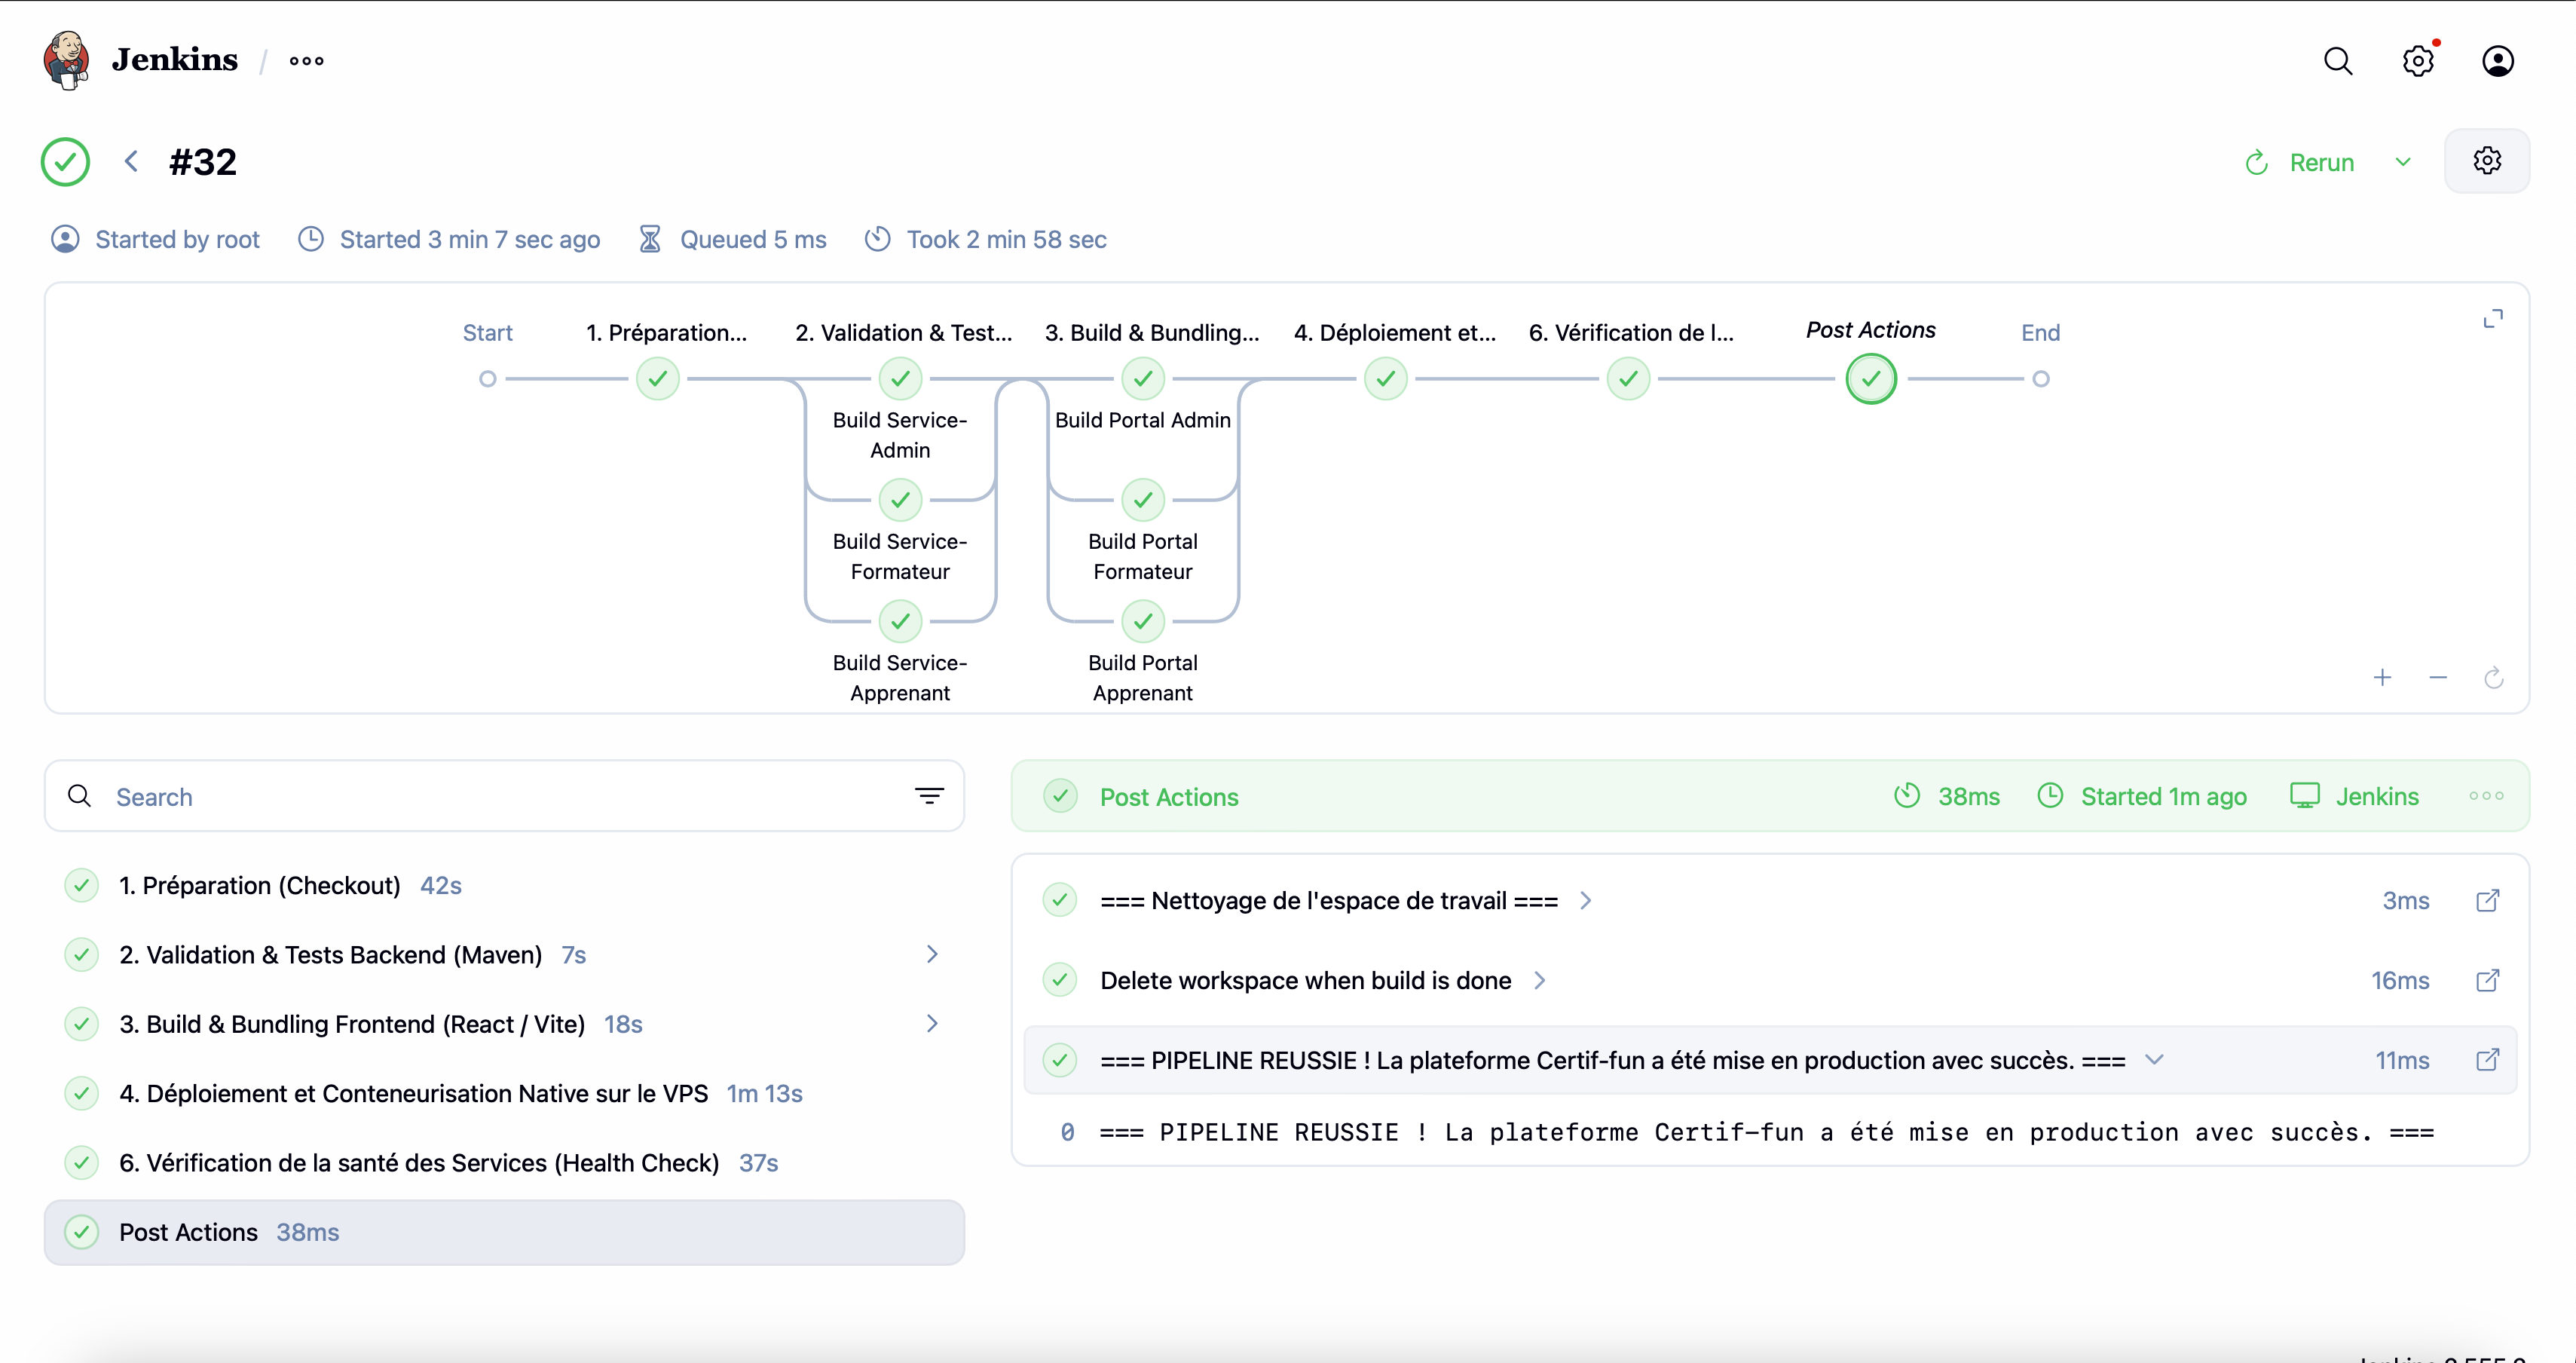
\includegraphics[width=0.98\textwidth]{figures/jenkins_pipeline.png}
    \caption{Interface de suivi visuel Jenkins présentant le succès de la build \#32 et le détail d'exécution séquentiel et parallèle des étapes du pipeline CI/CD.}
    \label{fig:jenkins_pipeline}
\end{figure}


\begin{enumerate}
    \item \textbf{Préparation [42s] :} Récupération sécurisée du code source via SSH et configuration automatique des environnements Node.js et Maven. Cette étape garantit un espace de build stable, portable et reproductible pour l'ensemble du projet. Elle permet de s'assurer que toutes les dépendances système sont prêtes avant le début de la compilation.

    \item \textbf{Compilation Backend [7s] :} Construction simultanée des trois microservices Spring Boot en parallèle pour optimiser les ressources. Cette méthode de compilation distribuée réduit drastiquement le temps de traitement global sur le serveur de build. Elle génère les artifacts exécutables nécessaires au déploiement des services métiers.

    \item \textbf{Compilation Frontend [18s] :} Génération et optimisation des trois interfaces React à l'aide du bundler Vite. Les fichiers statiques sont ainsi préparés et compressés pour une diffusion ultra-rapide sur le serveur web de production. Cette étape inclut la validation du typage TypeScript pour garantir la robustesse des interfaces.

    \item \textbf{Déploiement sur le VPS [1m 13s] :} Transfert de l'archive vers le serveur de production et mise à jour des conteneurs via Docker Compose. Une sauvegarde automatique de la base de données PostgreSQL est effectuée avant chaque mise à jour pour prévenir toute perte de données. Enfin, un nettoyage des images Docker orphelines libère l'espace disque du serveur.

    \item \textbf{Vérification de santé (Health Check) [37s] :} Contrôle automatique de la disponibilité des services via des requêtes sur les endpoints Actuator et la passerelle Nginx. Le pipeline s'interrompt immédiatement en cas d'anomalie détectée pour garantir la stabilité de la production. Cette étape valide que la nouvelle version est pleinement opérationnelle avant de clôturer la build.

    \item \textbf{Nettoyage local [< 1s] :} Purge complète de l'espace de travail sur l'agent Jenkins pour libérer les ressources disque après le succès du déploiement. Cette maintenance automatique évite l'encombrement du serveur de build sur le long terme. Elle assure que chaque nouveau pipeline démarre dans un environnement vierge et sain.
\end{enumerate}

Ce pipeline Jenkins assure des déploiements rapides, sécurisés et automatisés, garantissant l'intégrité et la disponibilité continue de la plateforme \textbf{Certif-fun}.


%%%%%%%%%%%%%%%%%%%%%%%%%%%%%%%%%%%%%%%%%%%%%%%%%%%%%%%%%%%
\section{Implémentation et interfaces}
%%%%%%%%%%%%%%%%%%%%%%%%%%%%%%%%%%%%%%%%%%%%%%%%%%%%%%%%%%%
L'implémentation de la plateforme \textbf{Certif-fun} est conçue selon un découpage strict des responsabilités en couches isolées, respectant le principe de séparation des préoccupations (\textit{Separation of Concerns}). Cette architecture se divise en trois couches principales : la présentation (Front-end), la logique métier (Back-end) et la persistance des données.

\subsection{Découpage architectural global}
Pour comprendre le fonctionnement global de la plateforme de manière simple, les requêtes transitent à travers les couches suivantes :
\begin{itemize}
    \item \textbf{Couche de Présentation (Front-end) :} Développée avec \textbf{React, TypeScript et Vite}. Elle fournit des interfaces fluides, interactives et responsives pour les trois types d'utilisateurs. Elle communique avec le serveur via des requêtes HTTP asynchrones gérées par la bibliothèque \textbf{Axios}.
    \item \textbf{Couche Logique Métier (Back-end) :} Composée de trois microservices indépendants développés avec \textbf{Spring Boot} (Java 17). Chaque microservice gère un domaine fonctionnel précis de la plateforme. En parallèle, un microservice Python développé avec \textbf{FastAPI} orchestre le modèle de détection visuelle \textbf{YOLOv8} pour la surveillance d'examen (Proctoring).
    \item \textbf{Couche de Données (Persistance) :} Repose sur le système de gestion de base de données relationnelle \textbf{PostgreSQL}. La couche de persistance Java utilise \textbf{Spring Data JPA} (Hibernate) pour manipuler les données sous forme d'objets (mapping objet-relationnel), évitant d'écrire des requêtes SQL manuelles complexes.
\end{itemize}

\subsection{Structure et organisation du code Backend (Spring Boot)}
Chacun des microservices Java (Admin, Formateur et Apprenant) est organisé selon une architecture en couches standardisée pour faciliter sa maintenance :
\begin{itemize}
    \item \textbf{\texttt{config} (Configuration) :} Regroupe les classes de paramétrage global de l'application (configurations CORS, initialisation des données par défaut via \texttt{DataInitializer}, et beans système).
    \item \textbf{\texttt{controller} (Contrôleurs REST) :} Représente le point d'entrée des requêtes HTTP. Il définit les URLs des APIs (points de terminaison comme \path{/api/v1/courses}), intercepte les requêtes envoyées par le frontend React, valide les données reçues et renvoie les réponses au format JSON.
    \item \textbf{\texttt{service} (Logique Métier) :} C'est le cœur applicatif. Ce package contient les classes implémentant les règles fonctionnelles (calculs de progression, traitement des examens, validation d'éligibilité aux certificats, cryptage de mots de passe, et dialogues avec le serveur de visioconférence LiveKit ou avec l'IA Ollama).
    \item \textbf{\texttt{repository} (Accès aux Données) :} Contient les interfaces de persistance héritant de \texttt{JpaRepository}. Elles permettent d'exécuter des opérations de lecture et d'écriture (CRUD) dans la base de données PostgreSQL de manière abstraite.
    \item \textbf{\texttt{model} (Entités) :} Définit les classes Java annotées avec \texttt{@Entity} représentant la structure de nos tables PostgreSQL (ex. \texttt{Course}, \texttt{Quiz}, \texttt{Apprenant}, \texttt{EncadrementPhase}).
    \item \textbf{\texttt{dto} (Data Transfer Objects) :} Classes simples utilisées pour structurer les données transférées entre le frontend et le backend (ex. \texttt{AuthenticationRequest}, \texttt{QuizStatisticsDTO}), permettant de ne pas exposer directement les entités de la base de données.
    \item \textbf{\texttt{security} (Sécurité JWT) :} Contient le filtre \texttt{JwtAuthenticationFilter} qui extrait et valide le jeton de connexion des requêtes entrantes pour authentifier l'utilisateur.
\end{itemize}

\subsection{Structure et organisation du code Frontend (React)}
Les trois applications frontales (\texttt{Service Admin}, \texttt{Service Formateur} et \texttt{Service Apprenant}) adoptent une structure modulaire, claire et réutilisable :
\begin{itemize}
    \item \textbf{\texttt{pages/} (Vues Principales) :} Contient les composants représentant les pages entières de l'application (ex. \path{Dashboard.tsx}, \path{Examen.tsx}, \path{Parametres.tsx}).
    \item \textbf{\texttt{components/} (Éléments UI Réutilisables) :} Regroupe les blocs visuels génériques et autonomes réutilisés sur plusieurs pages (boutons stylisés, barres de progression, modales d'alertes, cartes d'affichage de cours).
    \item \textbf{\texttt{api/} (Connexion API) :} Regroupe les configurations d'Axios, les intercepteurs pour ajouter automatiquement le token JWT dans les en-têtes HTTP de chaque requête, et les fonctions d'appel aux microservices backend.
    \item \textbf{\texttt{context/} (Gestion d'État Global) :} Contient les contextes React (ex. \texttt{AuthContext}) permettant de partager des informations globales (comme l'état de connexion de l'utilisateur ou ses droits d'accès) à l'ensemble des pages.
    \item \textbf{\texttt{hooks/} (Hooks Personnalisés) : } Fichiers encapsulant de la logique réutilisable (gestion du flux de la caméra web pour le proctoring, sélection de périphériques média).
    \item \textbf{\texttt{types/} (Typages TypeScript) :} Contient les interfaces TypeScript décrivant la forme des données reçues des API pour sécuriser l'écriture du code (auto-complétion, détection précoce d'erreurs de typage).
\end{itemize}

\subsection{Structure du service de traitement d'images (IA Proctoring)}
Le dossier \path{AI-Detection-Service} est structuré de façon minimale pour optimiser la rapidité d'exécution du traitement vidéo :
\begin{itemize}
    \item \textbf{\texttt{main.py} (Script principal) :} Initialise le serveur FastAPI, charge le modèle pré-entraîné YOLOv8 en mémoire (\texttt{yolov8n.pt}), et expose un point d'accès POST sécurisé. Il reçoit le flux d'images envoyé par le navigateur de l'apprenant sous format d'archive base64, décompresse l'image, applique les filtres de détection d'objets, et renvoie un dictionnaire JSON détaillant les anomalies identifiées (ex. détection de téléphone, nombre de visages).
    \item \textbf{\texttt{requirements.txt} (Dépendances Python) :} Liste les bibliothèques minimales nécessaires à l'exécution du service de vision par ordinateur (\texttt{fastapi}, \texttt{uvicorn}, \texttt{opencv-python-headless}, \texttt{ultralytics}).
\end{itemize}



\subsection{Interfaces utilisateur et scénarios de navigation}
L'ergonomie des interfaces de \textbf{Certif-fun} a été conçue pour offrir une expérience utilisateur (UX) fluide, immersive et moderne, articulée autour de trois portails distincts adaptés à chaque profil d'utilisateur. Dans cette section, nous présentons en détail les fonctionnalités offertes par chaque espace à travers des captures d'écran de l'application finale.

\subsubsection{Authentification et Accès}
Avant d'accéder aux différents portails, chaque utilisateur doit s'identifier.

La figure~\ref{fig:login} illustre la page de connexion sécurisée de la plateforme. Cette interface permet à l'utilisateur de s'authentifier en saisissant son adresse email et son mot de passe. Le système vérifie les identifiants et redirige l'utilisateur vers son espace dédié (Admin, Formateur ou Apprenant) en générant un jeton de session JWT.
\begin{figure}[H]
    \centering
    
\includegraphics[width=0.98\textwidth]{figures/login.png}
    \caption{Interface de connexion à la plateforme}
    \label{fig:login}
\end{figure}

\subsubsection{Portail Administrateur}
L'espace d'administration centralise les outils de supervision et de configuration de la plateforme.

La figure~\ref{fig:admin1} présente le tableau de bord principal de l'administrateur. Cette interface offre une vue d'ensemble instantanée sur l'activité de la plateforme à travers plusieurs indicateurs clés de performance :
\begin{itemize}
    \item \textbf{Total Apprenants :} Affiche le nombre total d'étudiants inscrits sur la plateforme.
    \item \textbf{Total Formateurs :} Indique le nombre de professeurs et encadrants actifs.
    \item \textbf{Taux de Réussite :} Présente le pourcentage moyen de réussite aux évaluations sur l'ensemble des cours.
    \item \textbf{Nombre Certificats :} Indique le nombre de certifications délivrées aux apprenants.
\end{itemize}
Un graphique interactif permet également de retracer l'évolution mensuelle des inscriptions.
\begin{figure}[H]
    \centering
    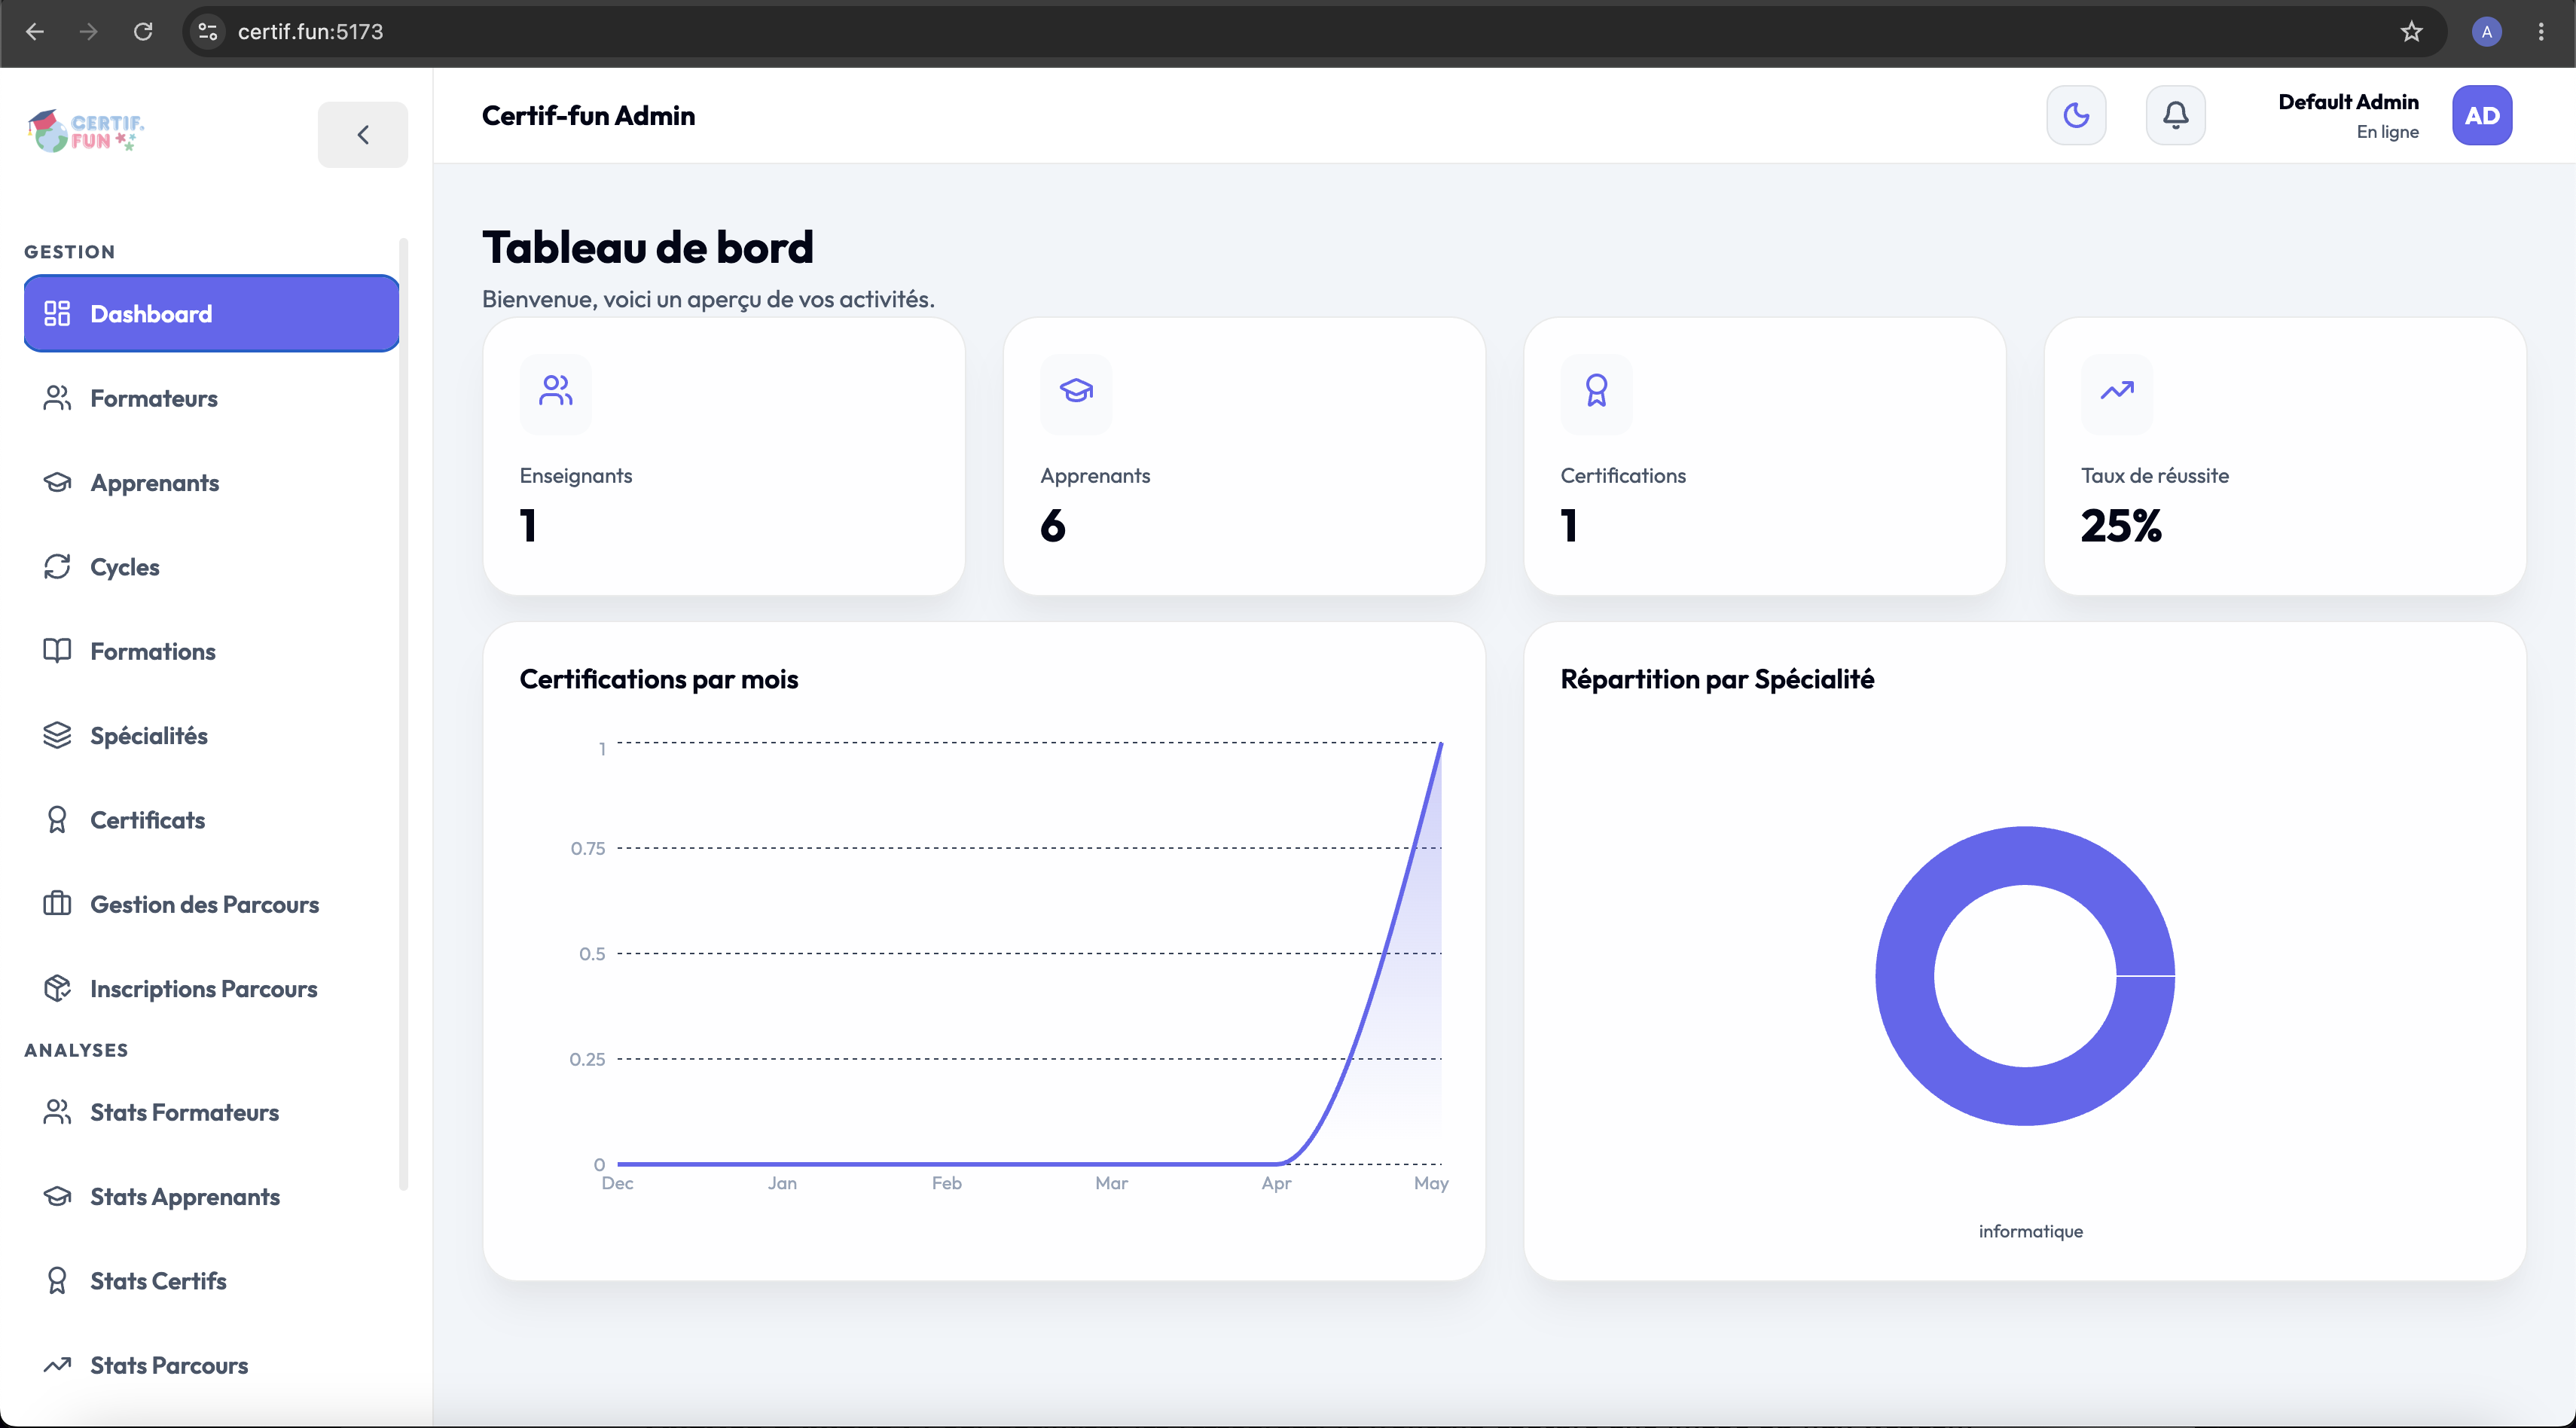
\includegraphics[width=0.98\textwidth]{figures/admin-1.png}
    \caption{Tableau de bord de l'Administrateur présentant les statistiques globales}
    \label{fig:admin1}
\end{figure}

La figure~\ref{fig:admin2} illustre le module de gestion des étudiants. L'administrateur dispose d'une liste complète des apprenants avec des outils de recherche rapide et de filtrage (par spécialité et statut). Il peut ajouter de nouveaux utilisateurs, modifier leurs informations ou restreindre leur accès si nécessaire. De plus, si l'apprenant est inséré correctement, il reçoit automatiquement un email pour s'authentifier à la plateforme.
\begin{figure}[H]
    \centering
    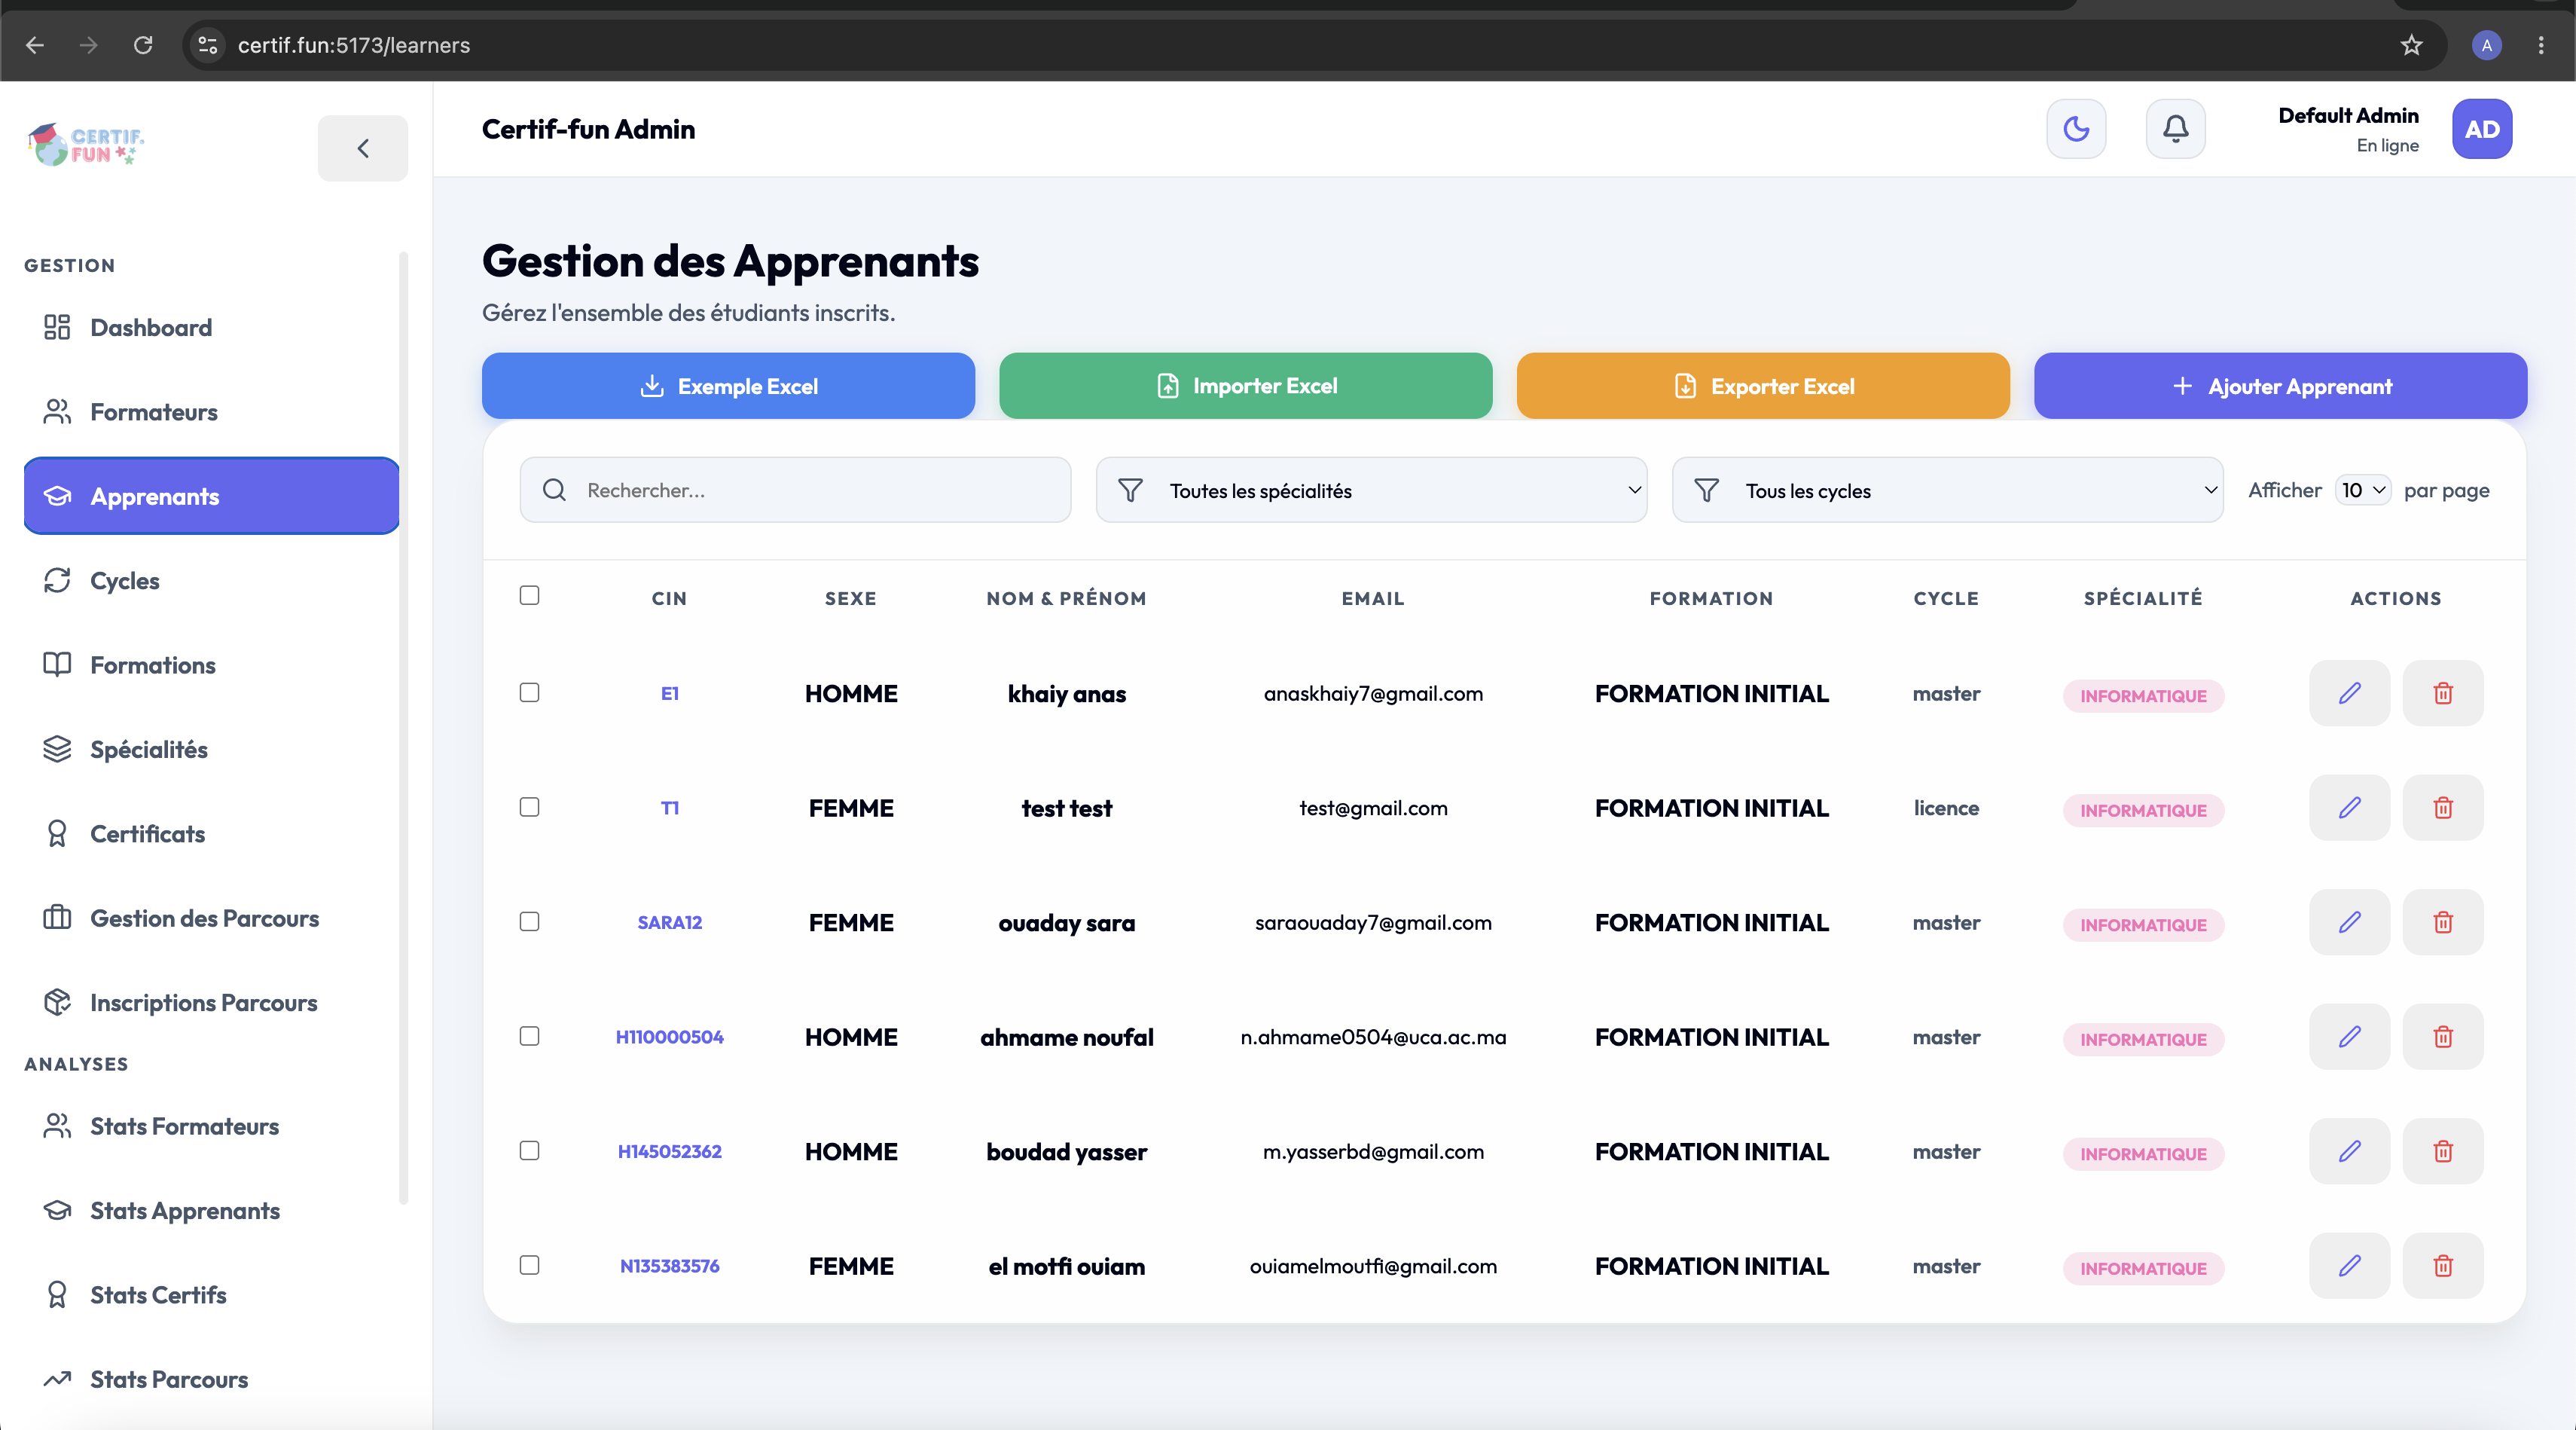
\includegraphics[width=0.98\textwidth]{figures/admin-2.png}
    \caption{Interface de gestion des étudiants}
    \label{fig:admin2}
\end{figure}

La section dédiée aux certificats (Figure~\ref{fig:admin3}) permet à l'administrateur d'ajuster le design des certificats, incluant le logo, la taille, le cachet et d'autres éléments visuels du certificat.
\begin{figure}[H]
    \centering
    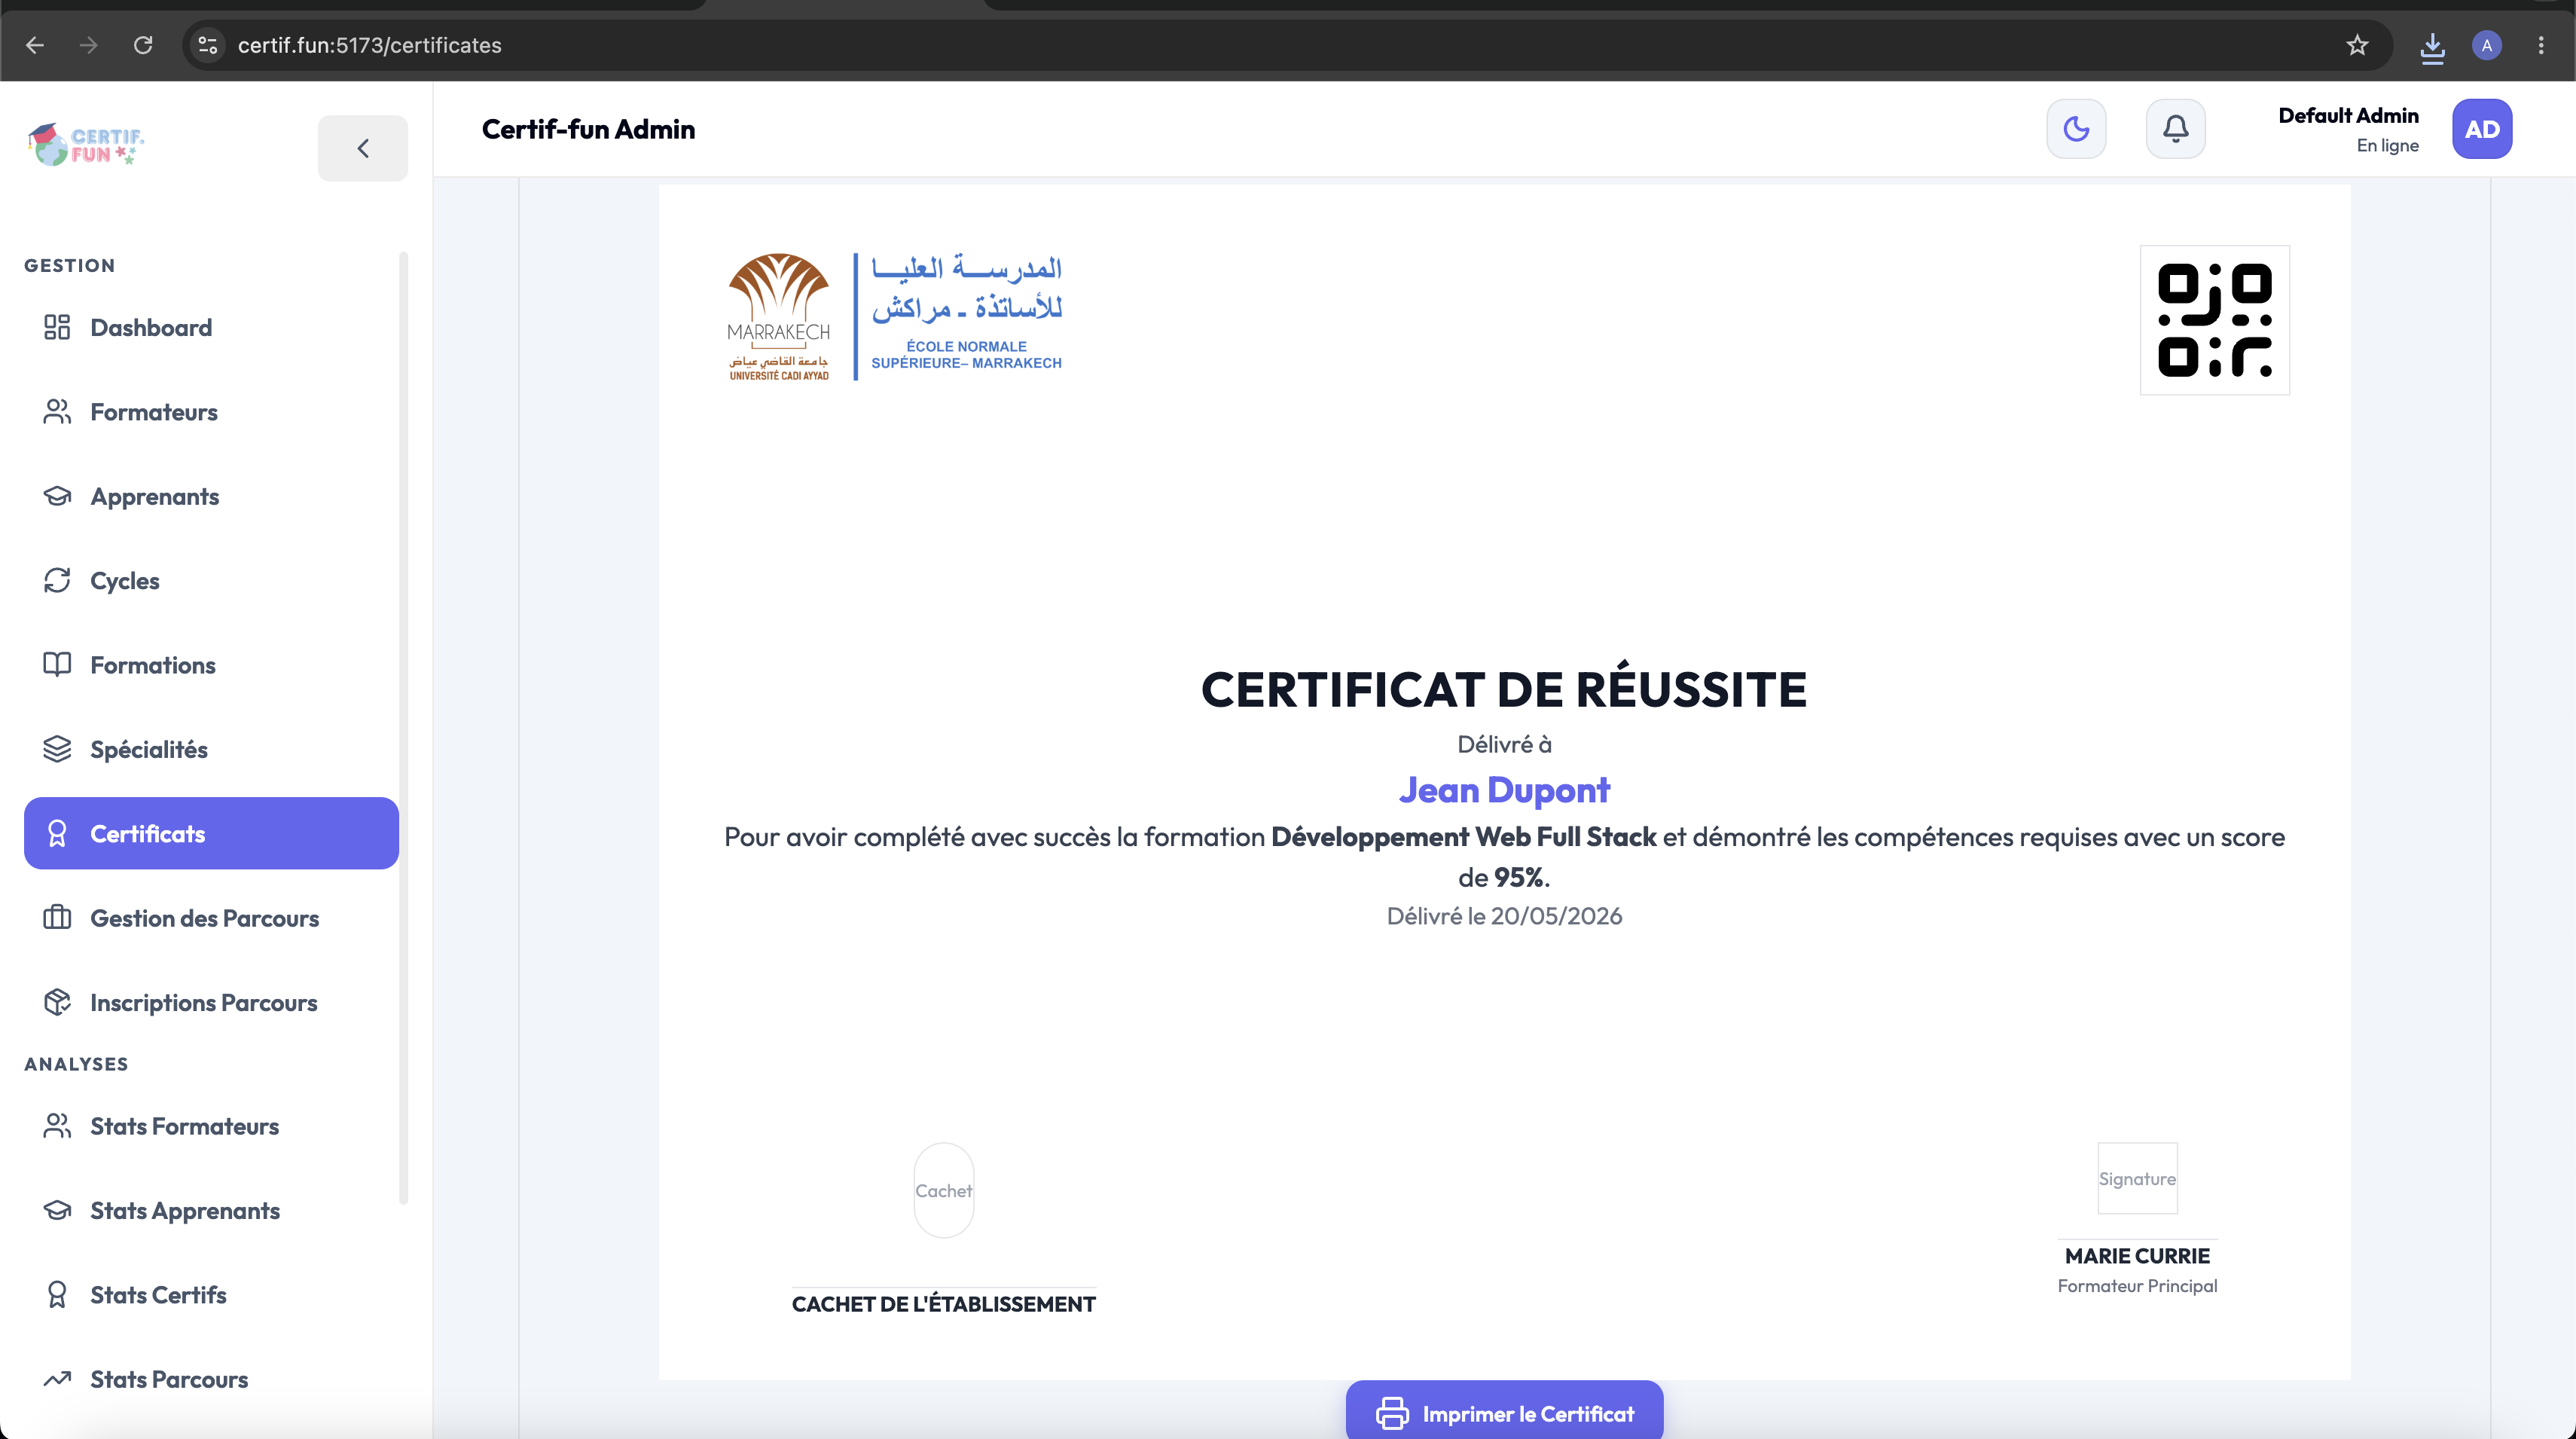
\includegraphics[width=0.98\textwidth]{figures/admin-3.png}
    \caption{Registre des certificats délivrés}
    \label{fig:admin3}
\end{figure}

La section dédiée aux parcours (Figure~\ref{fig:admin4}) permet aux formateurs de suivre un parcours qui contient plusieurs cours.
\begin{figure}[H]
    \centering
    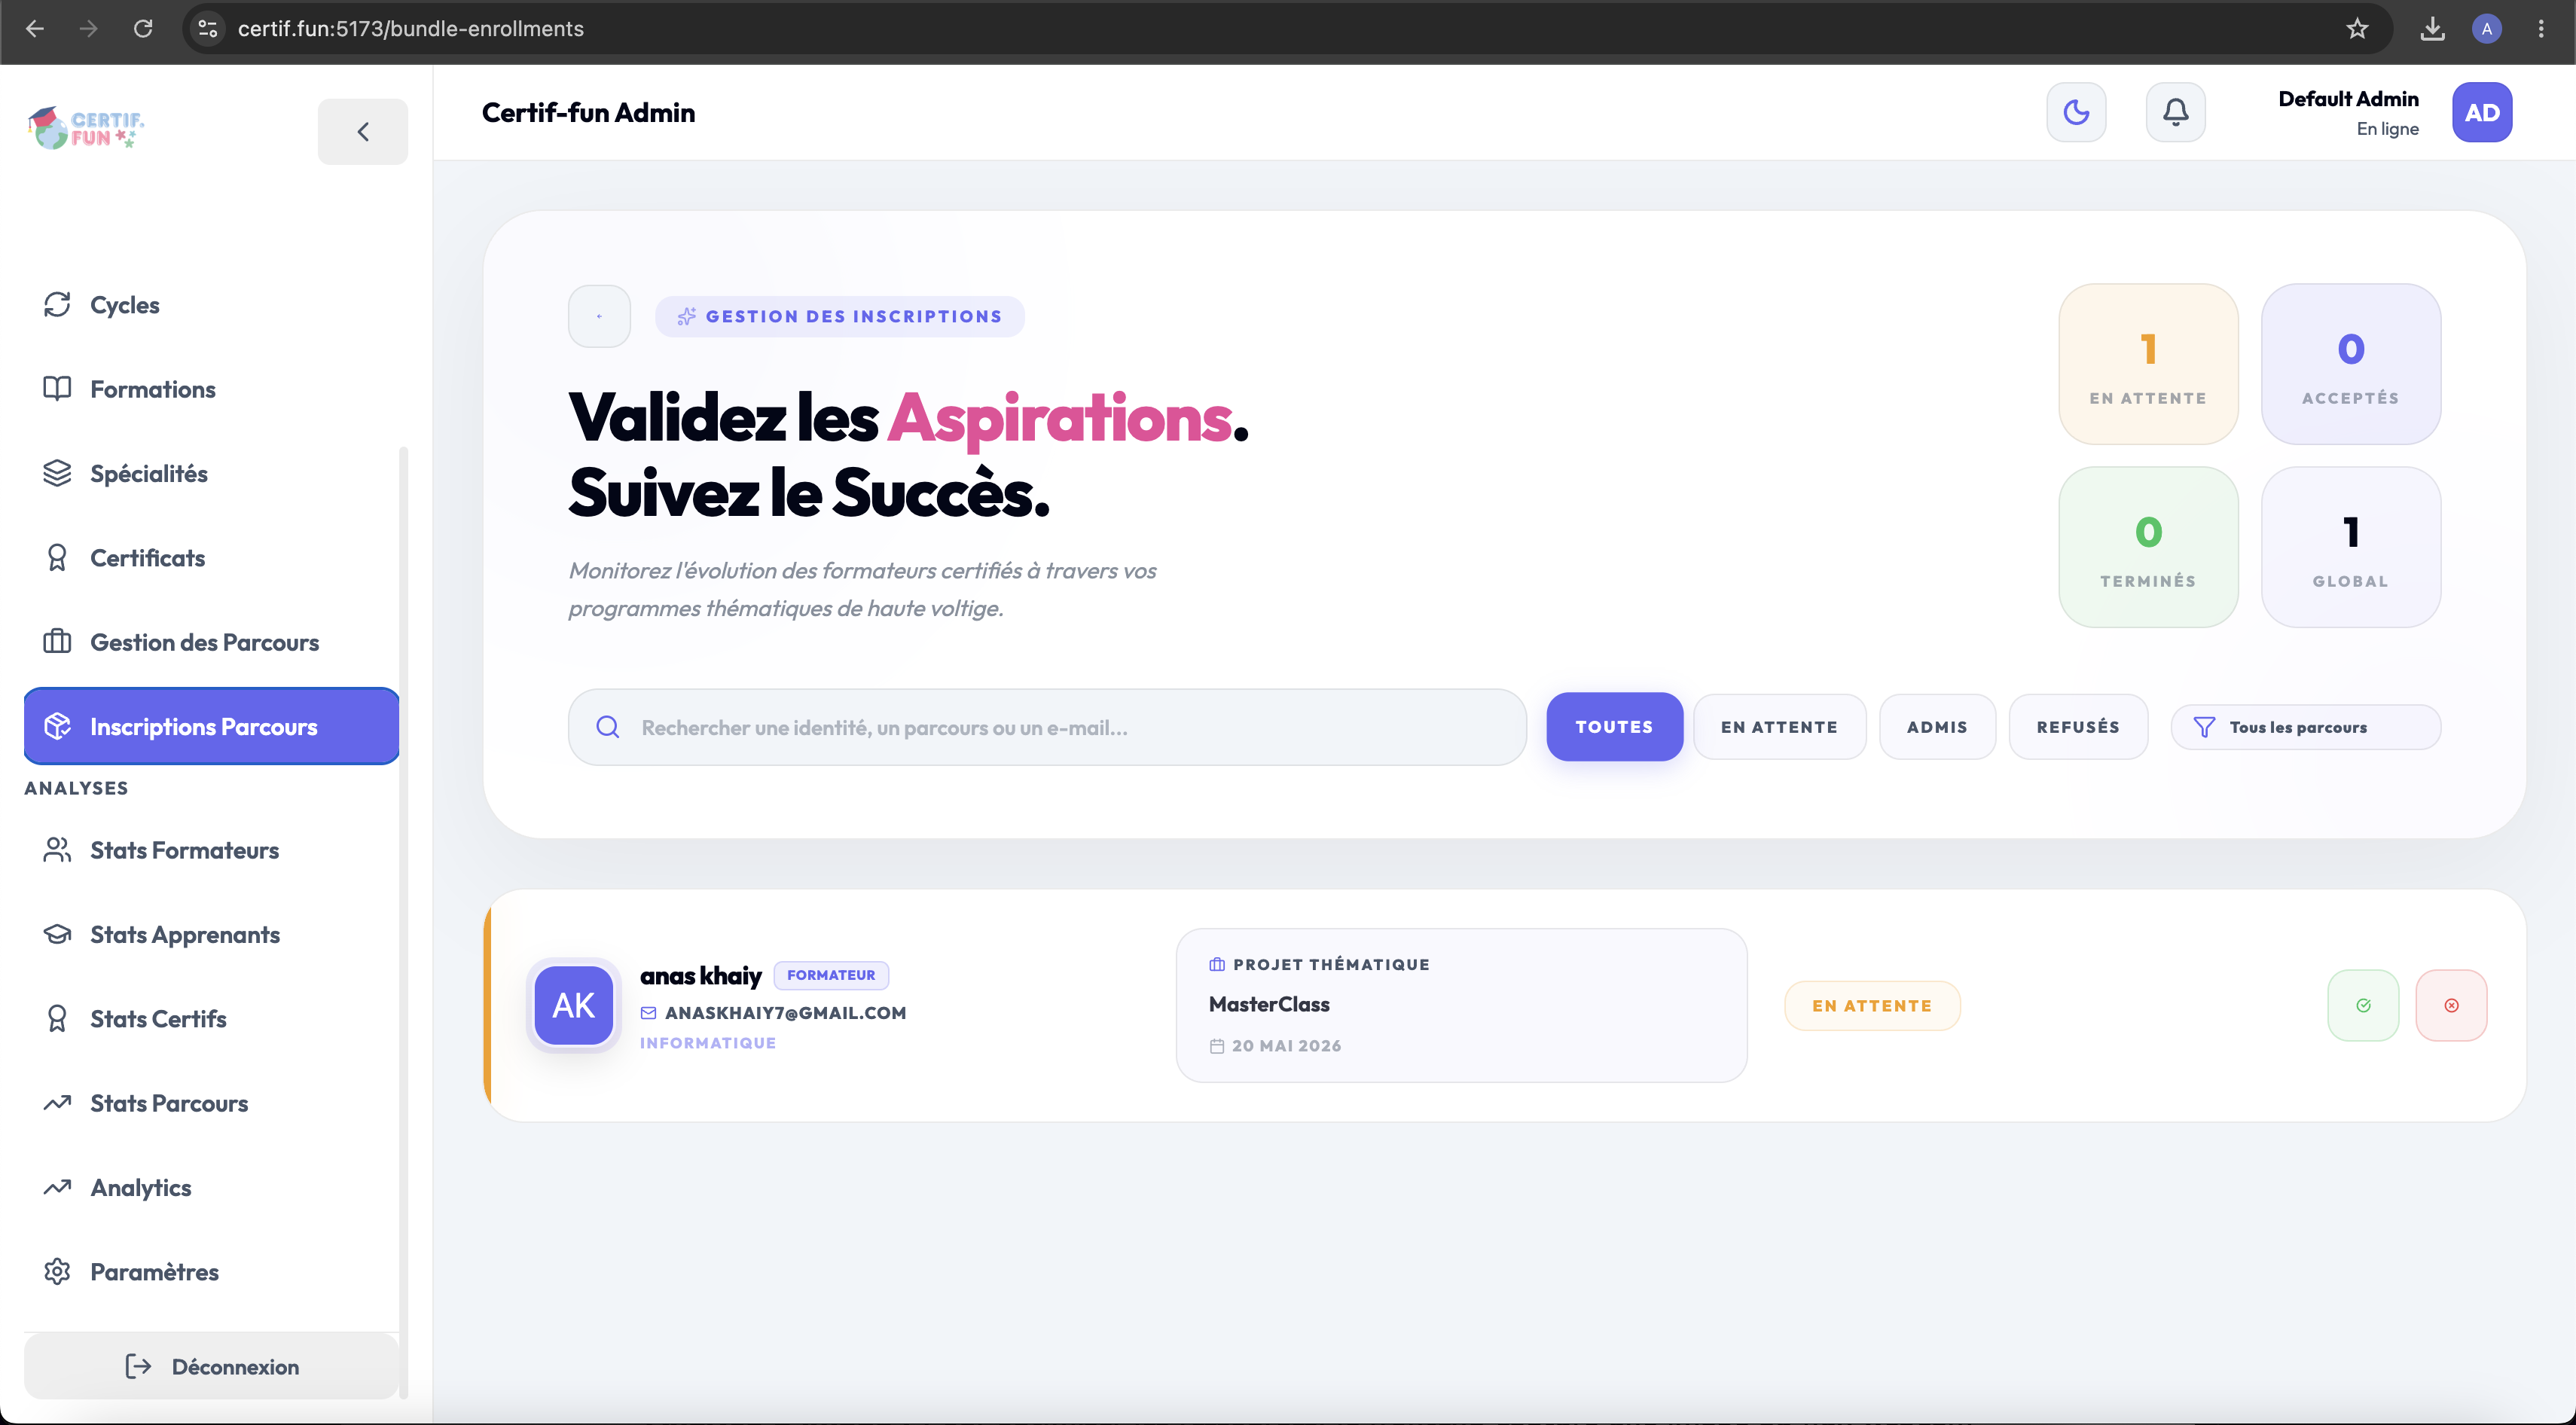
\includegraphics[width=0.98\textwidth]{figures/admin-4.png}
    \caption{Gestion des demandes d'inscription}
    \label{fig:admin4}
\end{figure}

\subsubsection{Portail Formateur}
L'espace Formateur est conçu pour faciliter la création de contenu pédagogique et le suivi des apprenants.

Le tableau de bord (Figure~\ref{fig:formateur1}) offre au formateur un résumé de son activité. Il y retrouve des statistiques sur ses apprenants, le taux de réussite global et le nombre de certificats délivrés aux étudiants.
\begin{figure}[H]
    \centering
    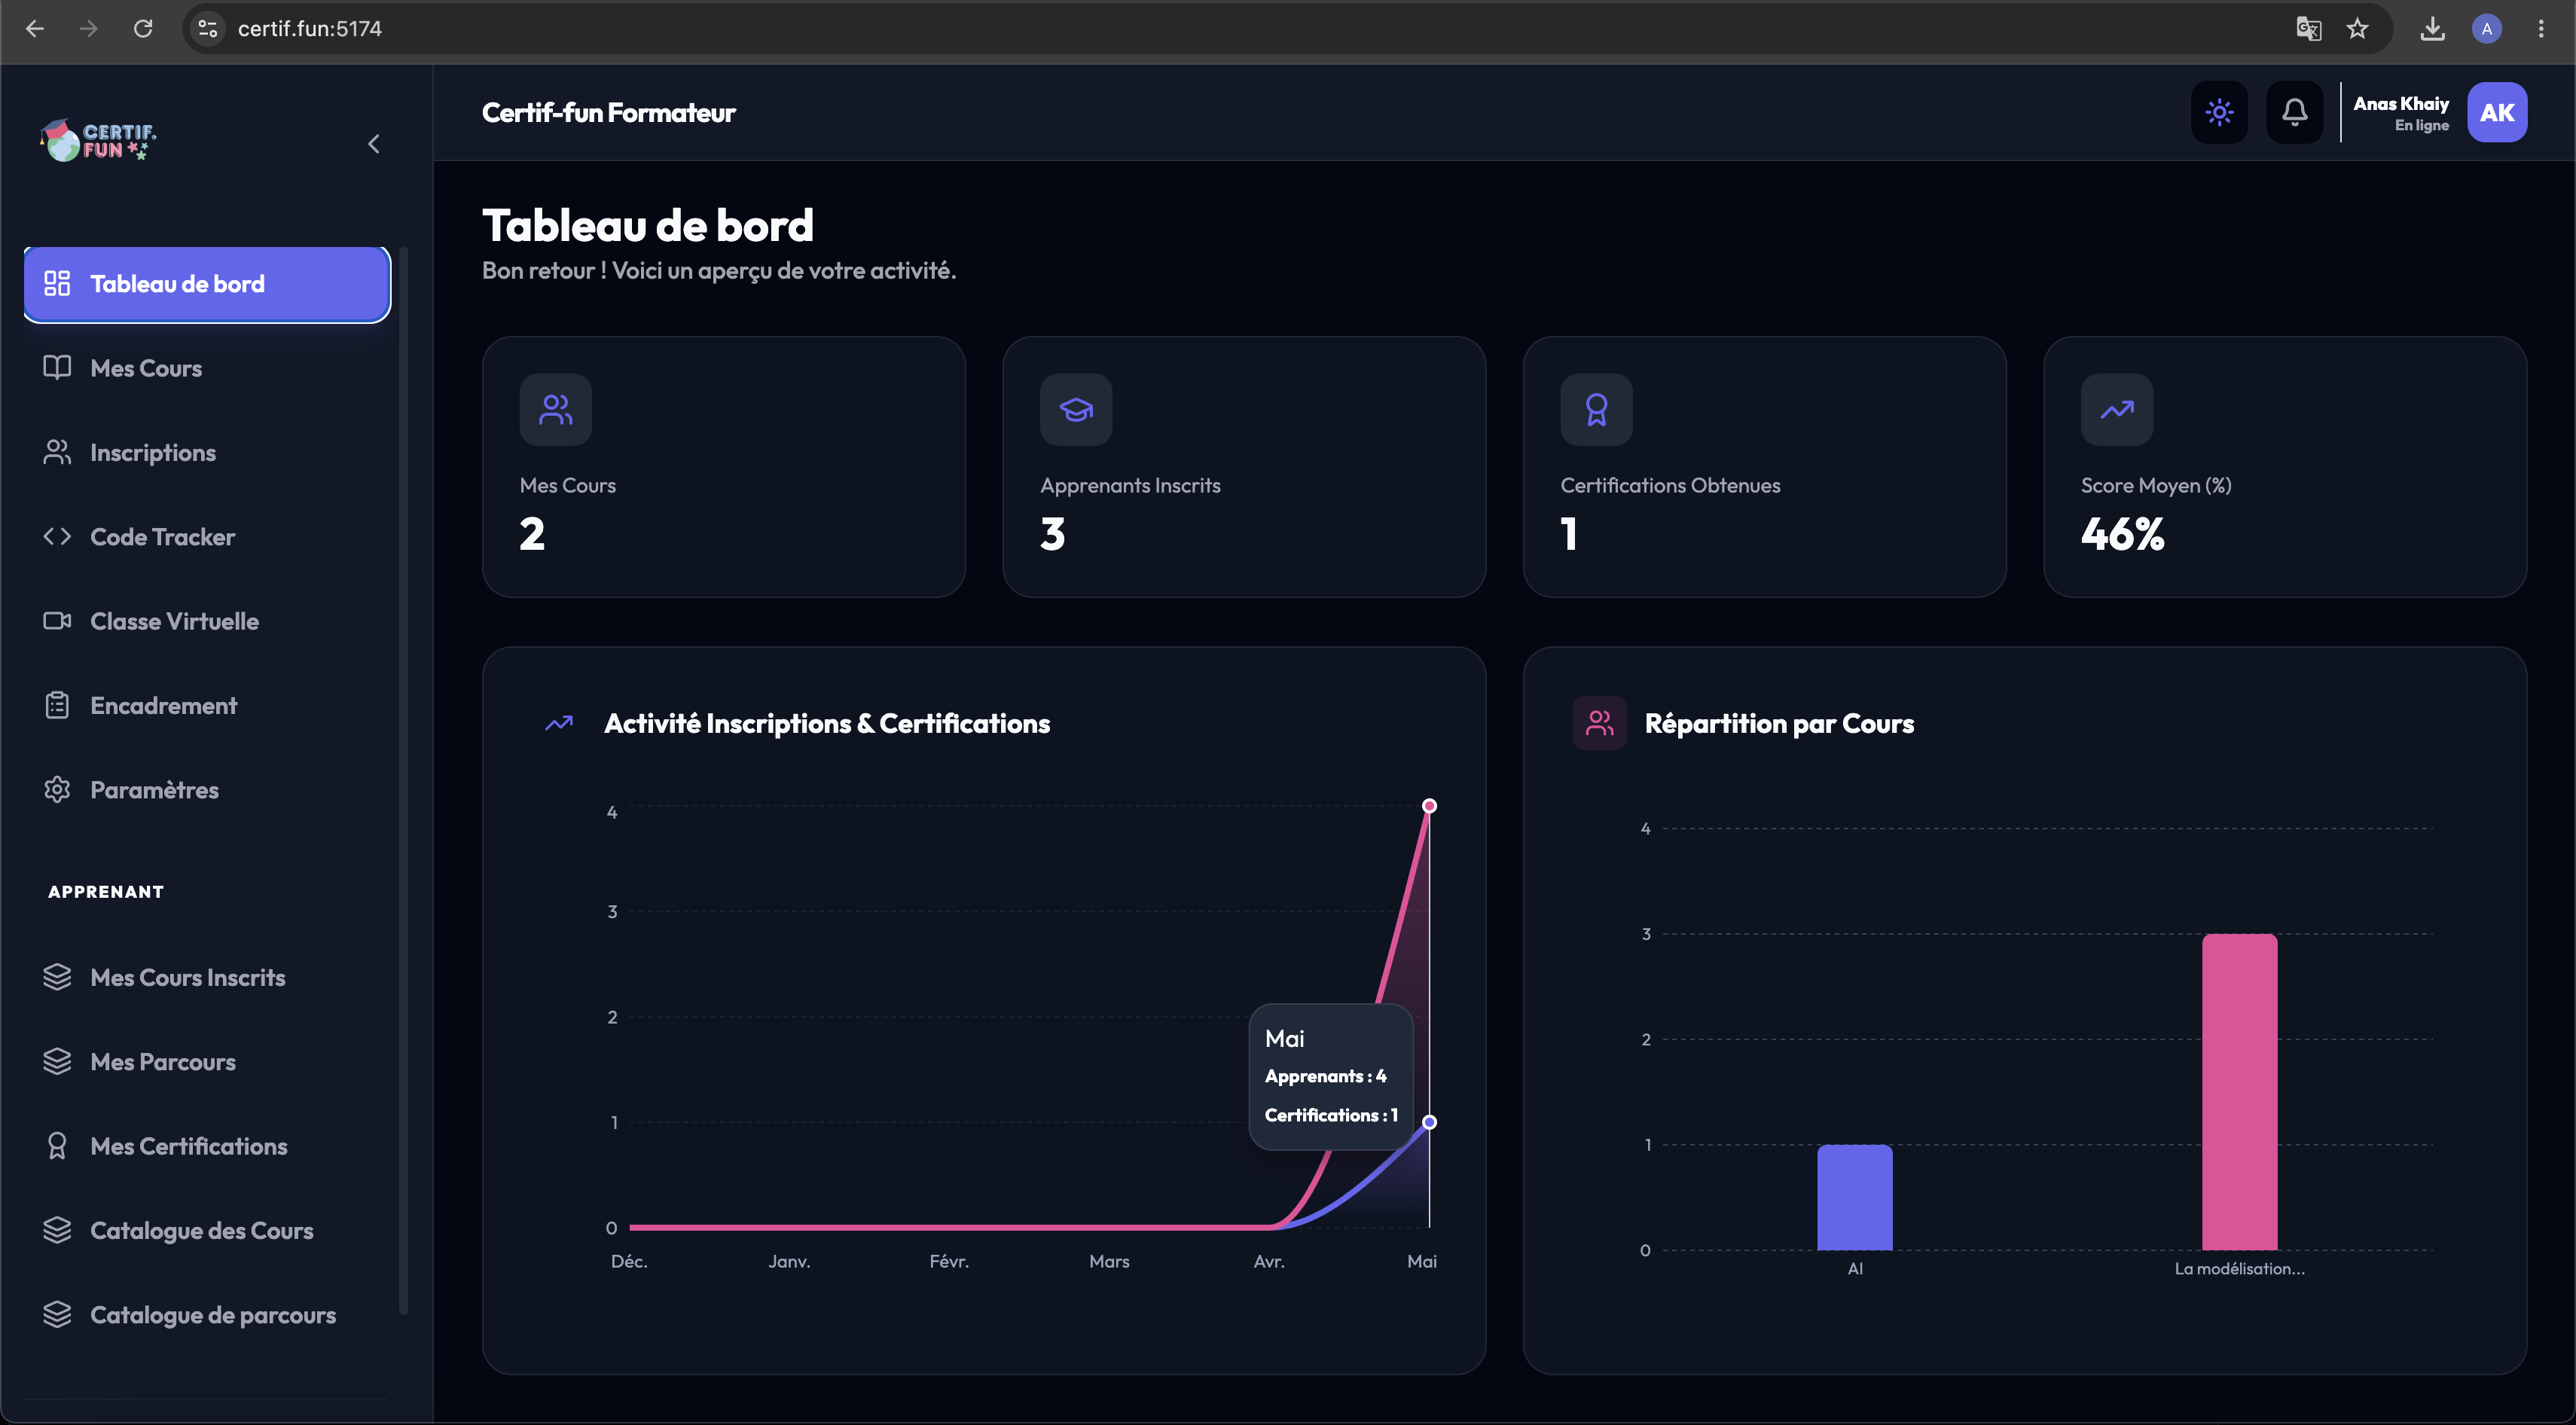
\includegraphics[width=0.98\textwidth]{figures/formateur-1.png}
    \caption{Tableau de bord du Formateur}
    \label{fig:formateur1}
\end{figure}

La vue "Mes Cours" (Figure~\ref{fig:formateur2}) permet au professeur de créer un cours avec plusieurs fonctionnalités avancées, telles que la définition d'une date limite pour finaliser la certification et un compteur pour afficher le nombre de minutes passées par l'apprenant dans la certification.
\begin{figure}[H]
    \centering
    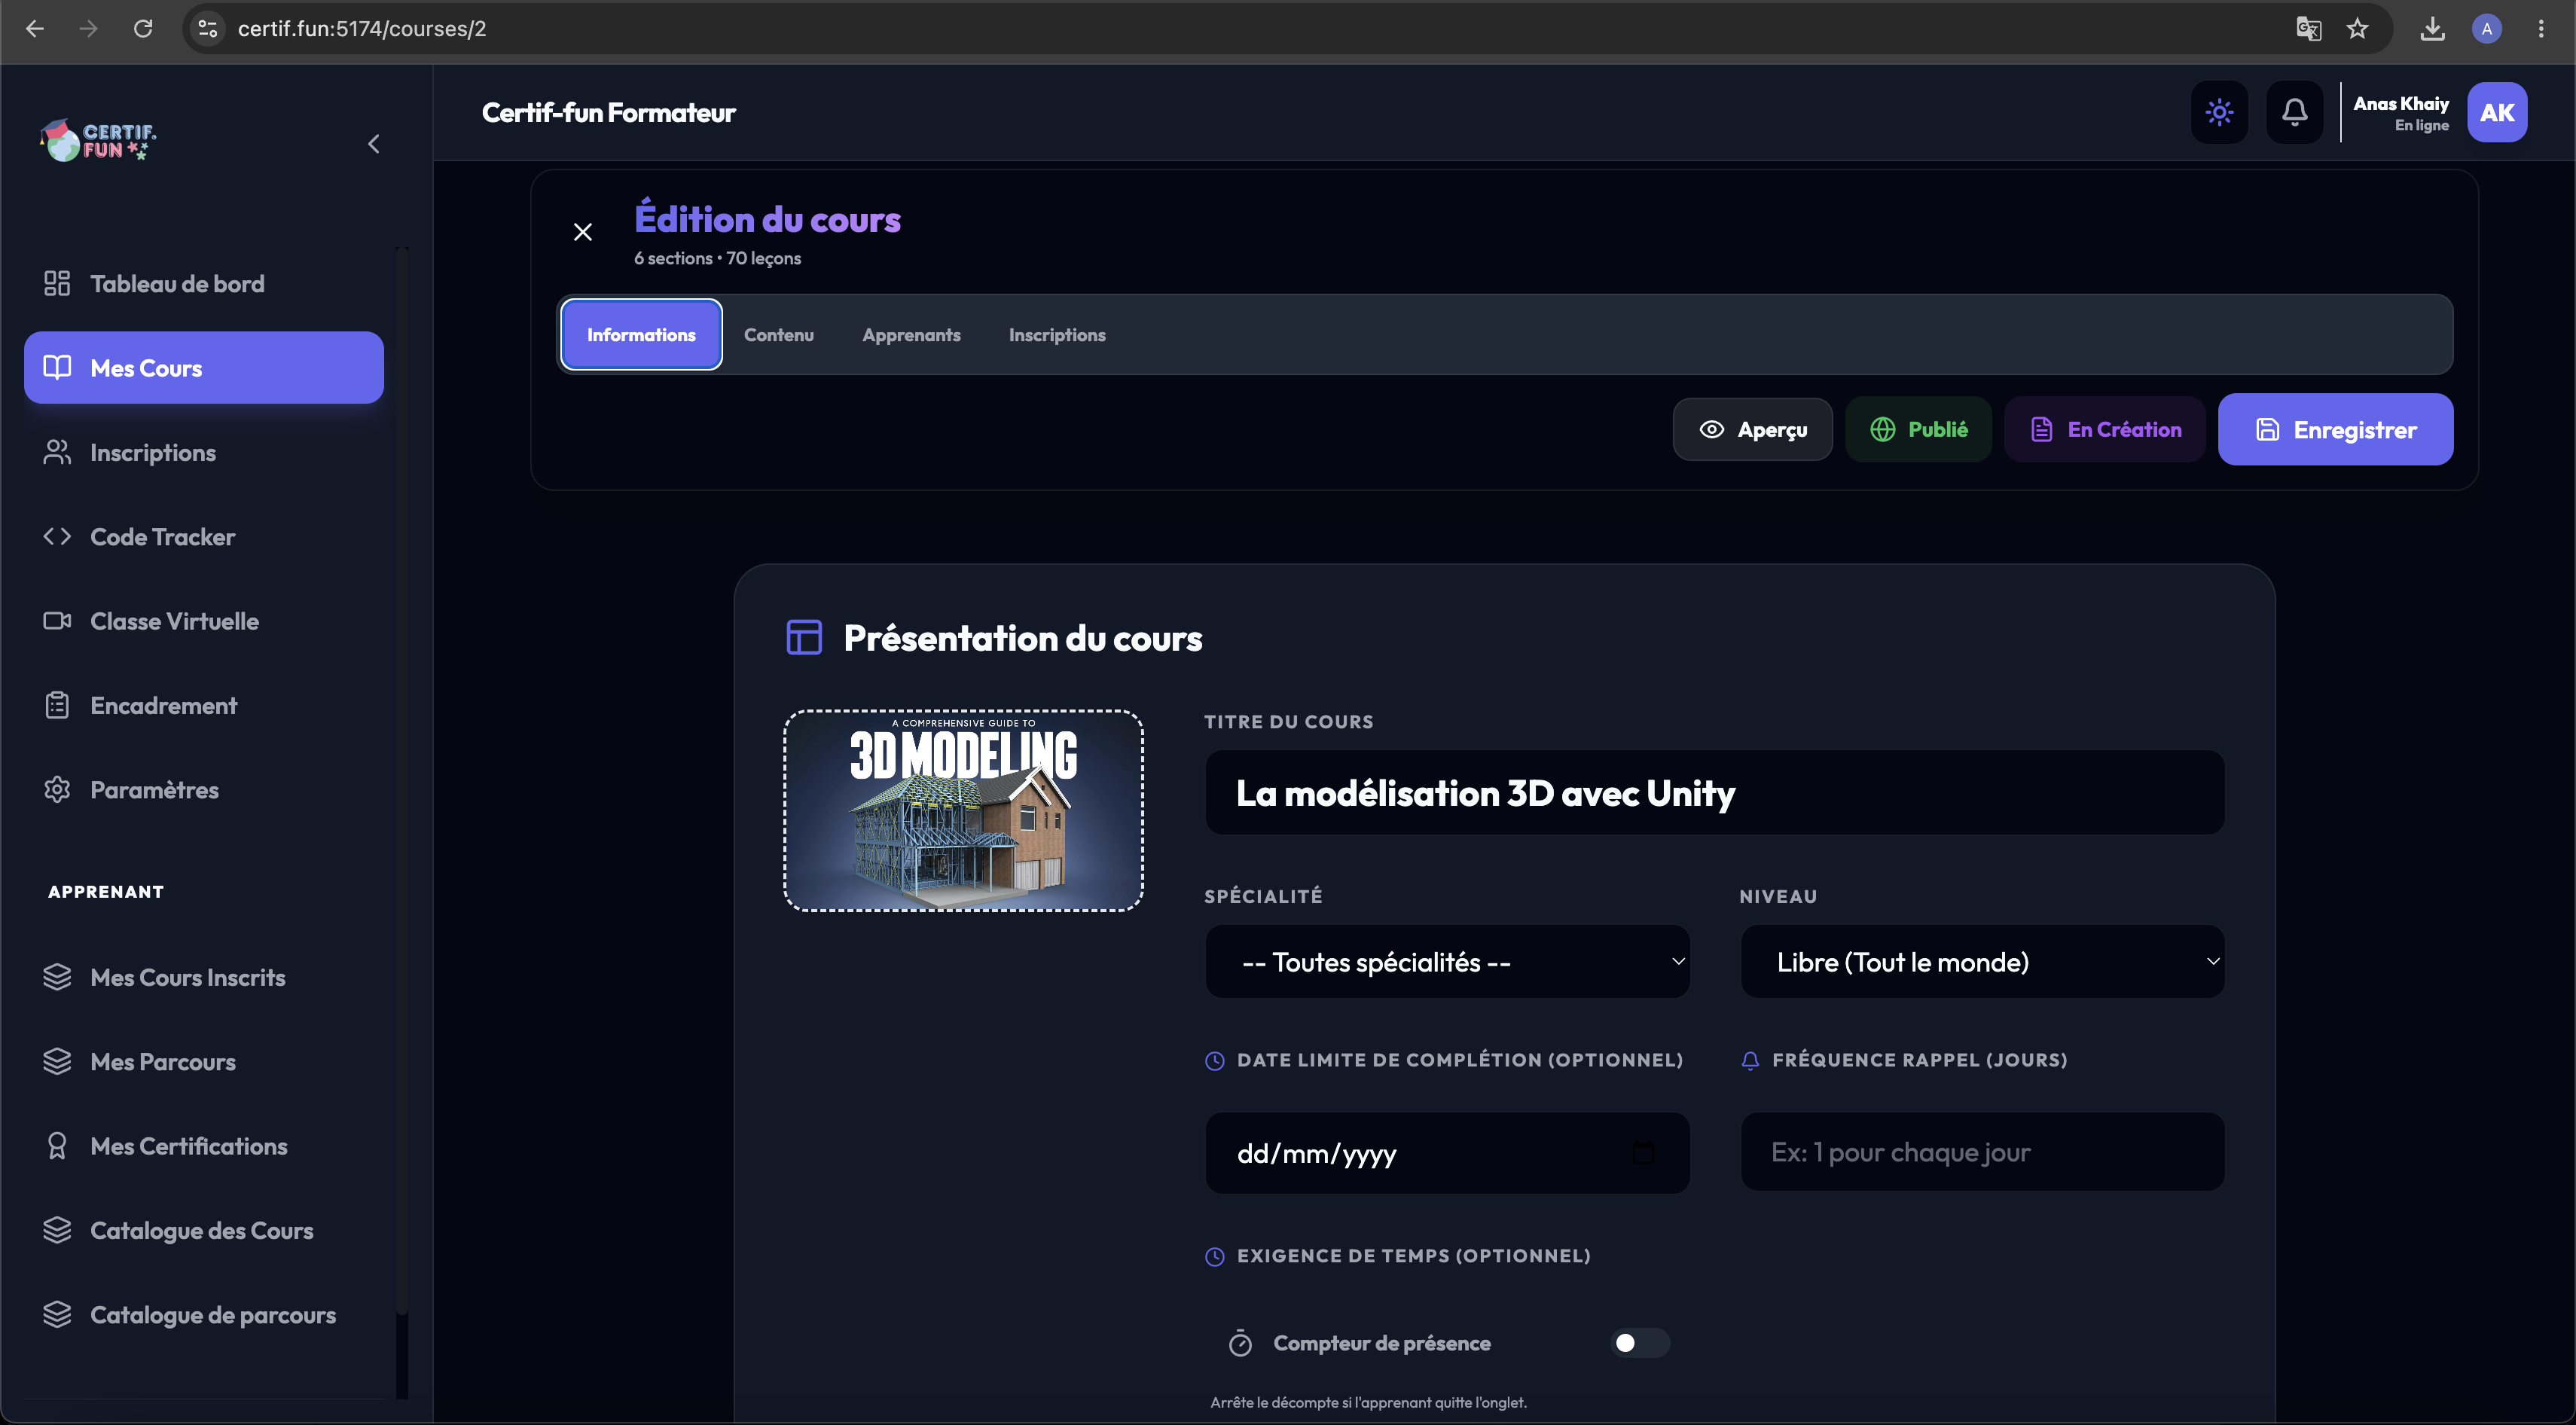
\includegraphics[width=0.98\textwidth]{figures/formateur-2.png}
    \caption{Liste des cours du formateur}
    \label{fig:formateur2}
\end{figure}

Lors de la création d'un nouveau cours (Figure~\ref{fig:formateur3}), le formateur peut structurer son cours en sections et en leçons. Ces leçons peuvent intégrer divers types de contenus tels que des vidéos, du texte, des images ou des quiz.
\begin{figure}[H]
    \centering
    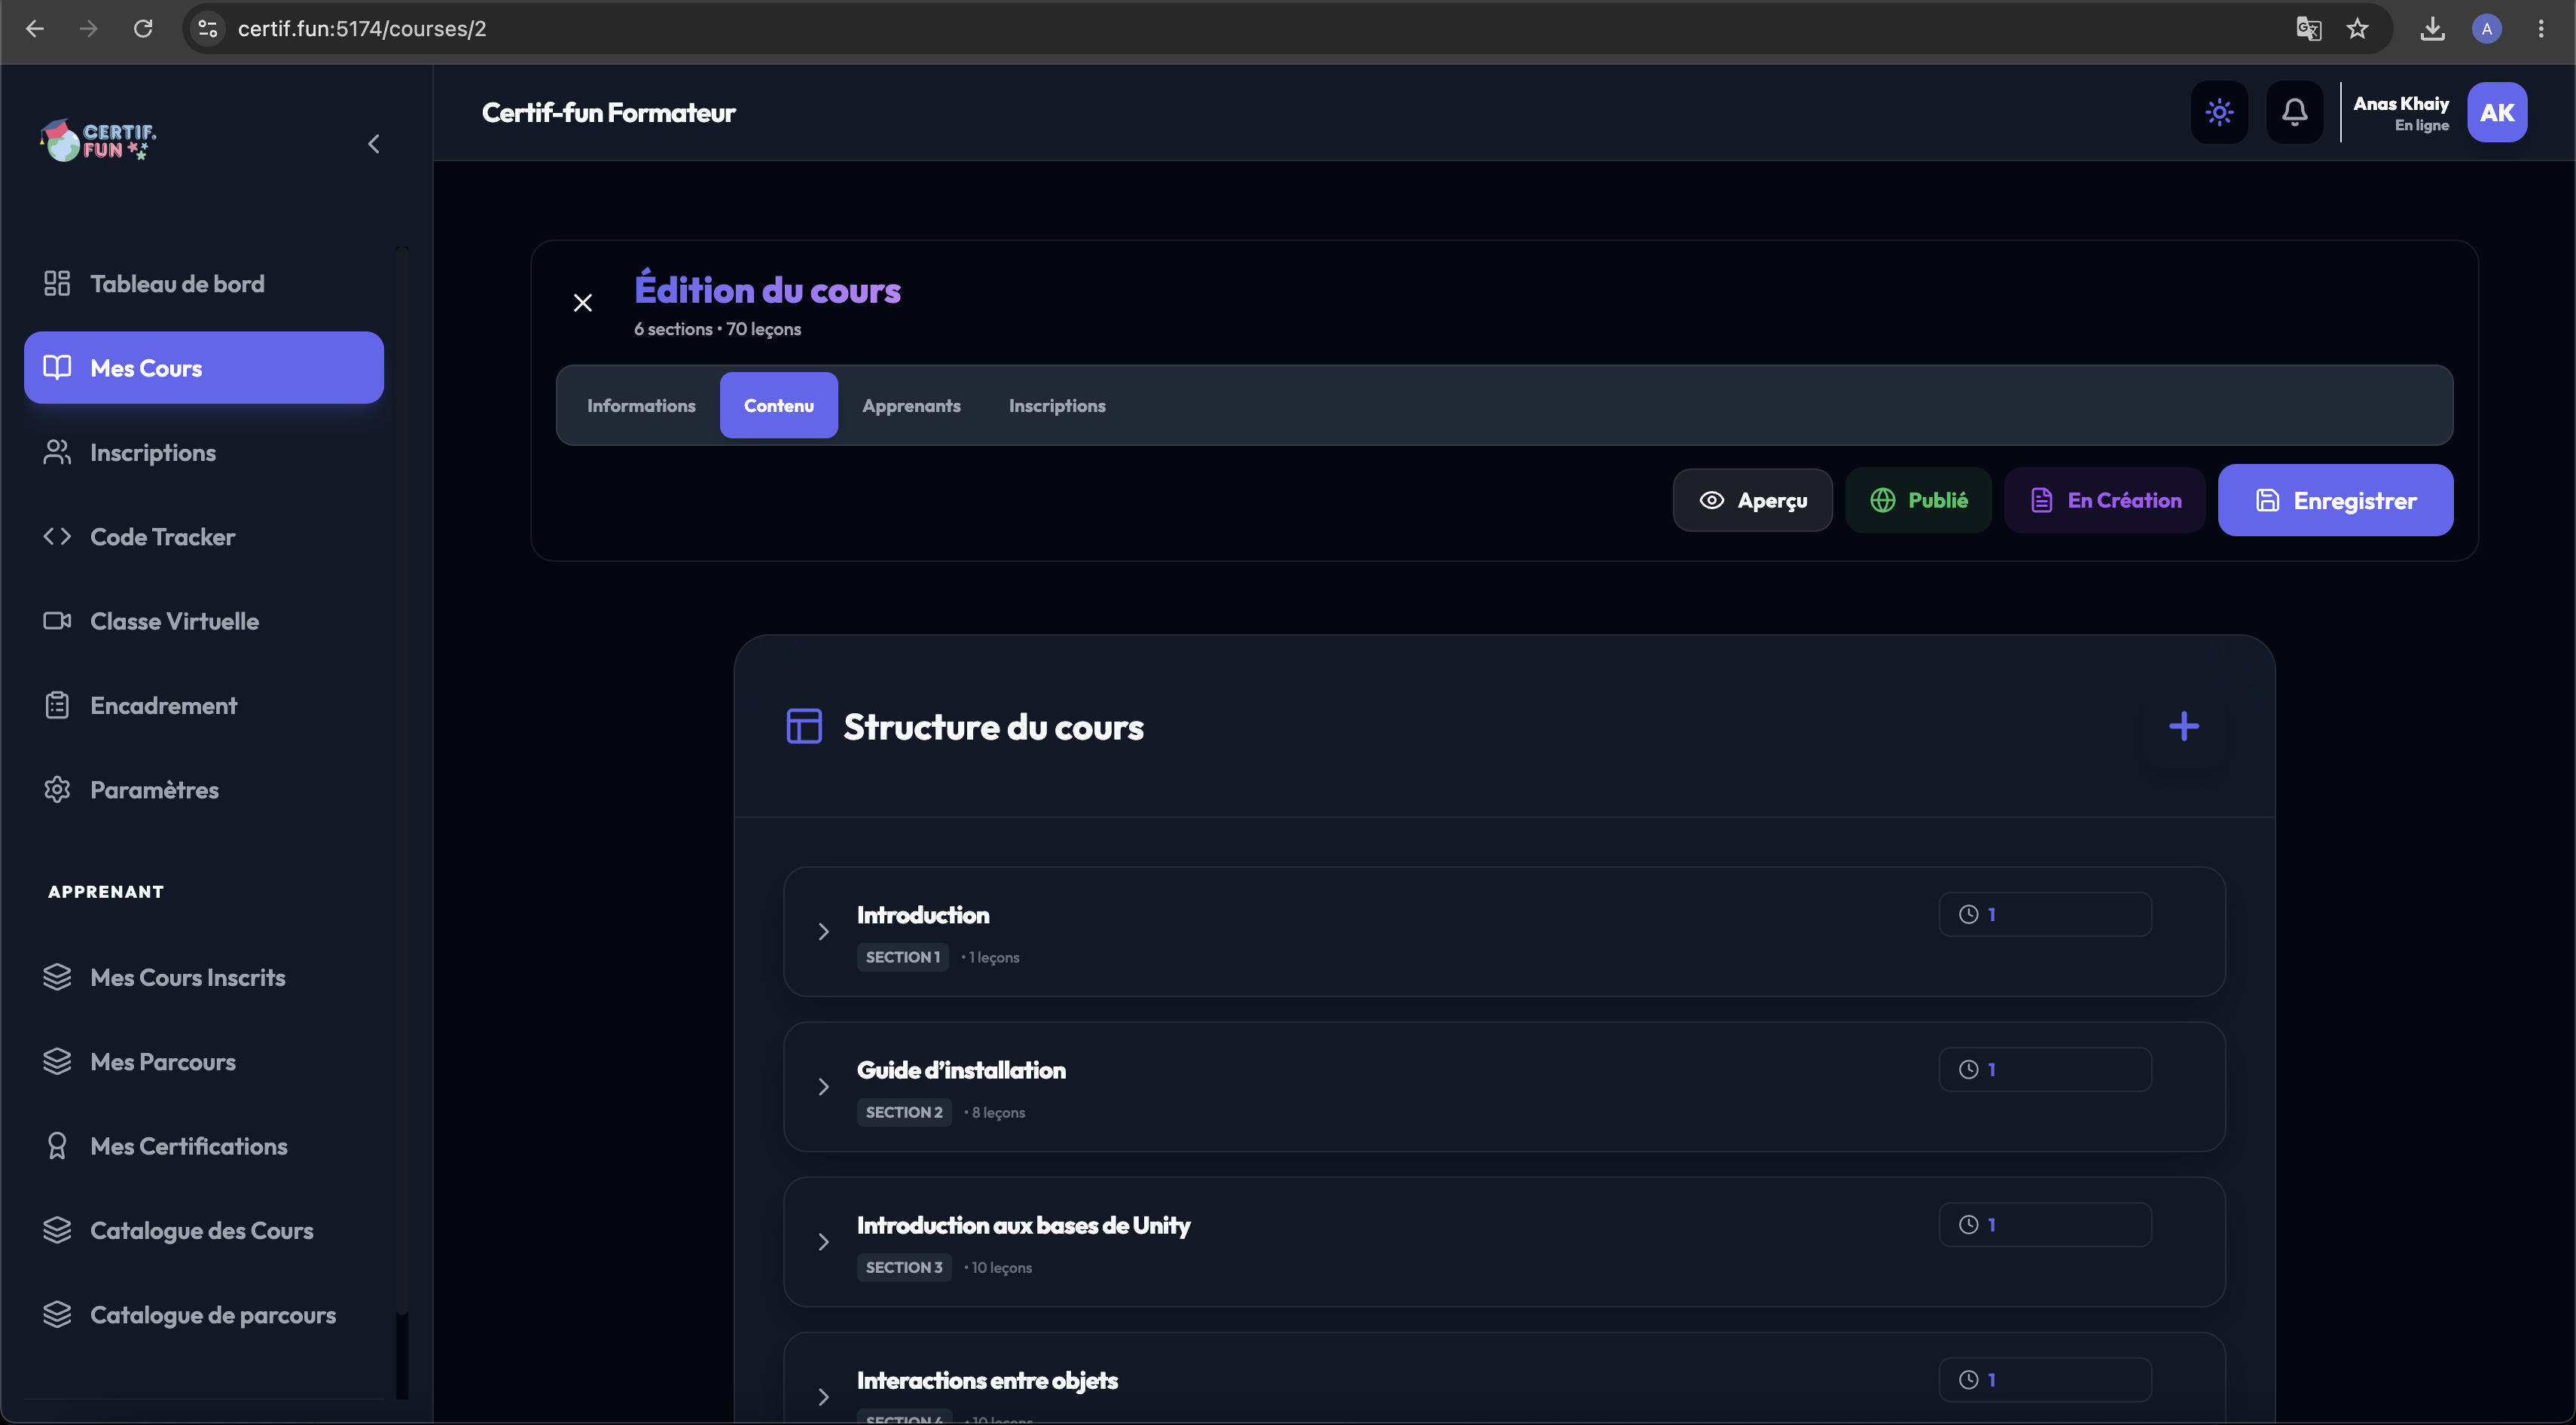
\includegraphics[width=0.98\textwidth]{figures/formateur-3.png}
    \caption{Formulaire de création d'un nouveau cours}
    \label{fig:formateur3}
\end{figure}

L'interface de suivi (Figure~\ref{fig:formateur4}) permet au formateur de visualiser la progression détaillée de chaque étudiant au sein de la formation.
\begin{figure}[H]
    \centering
    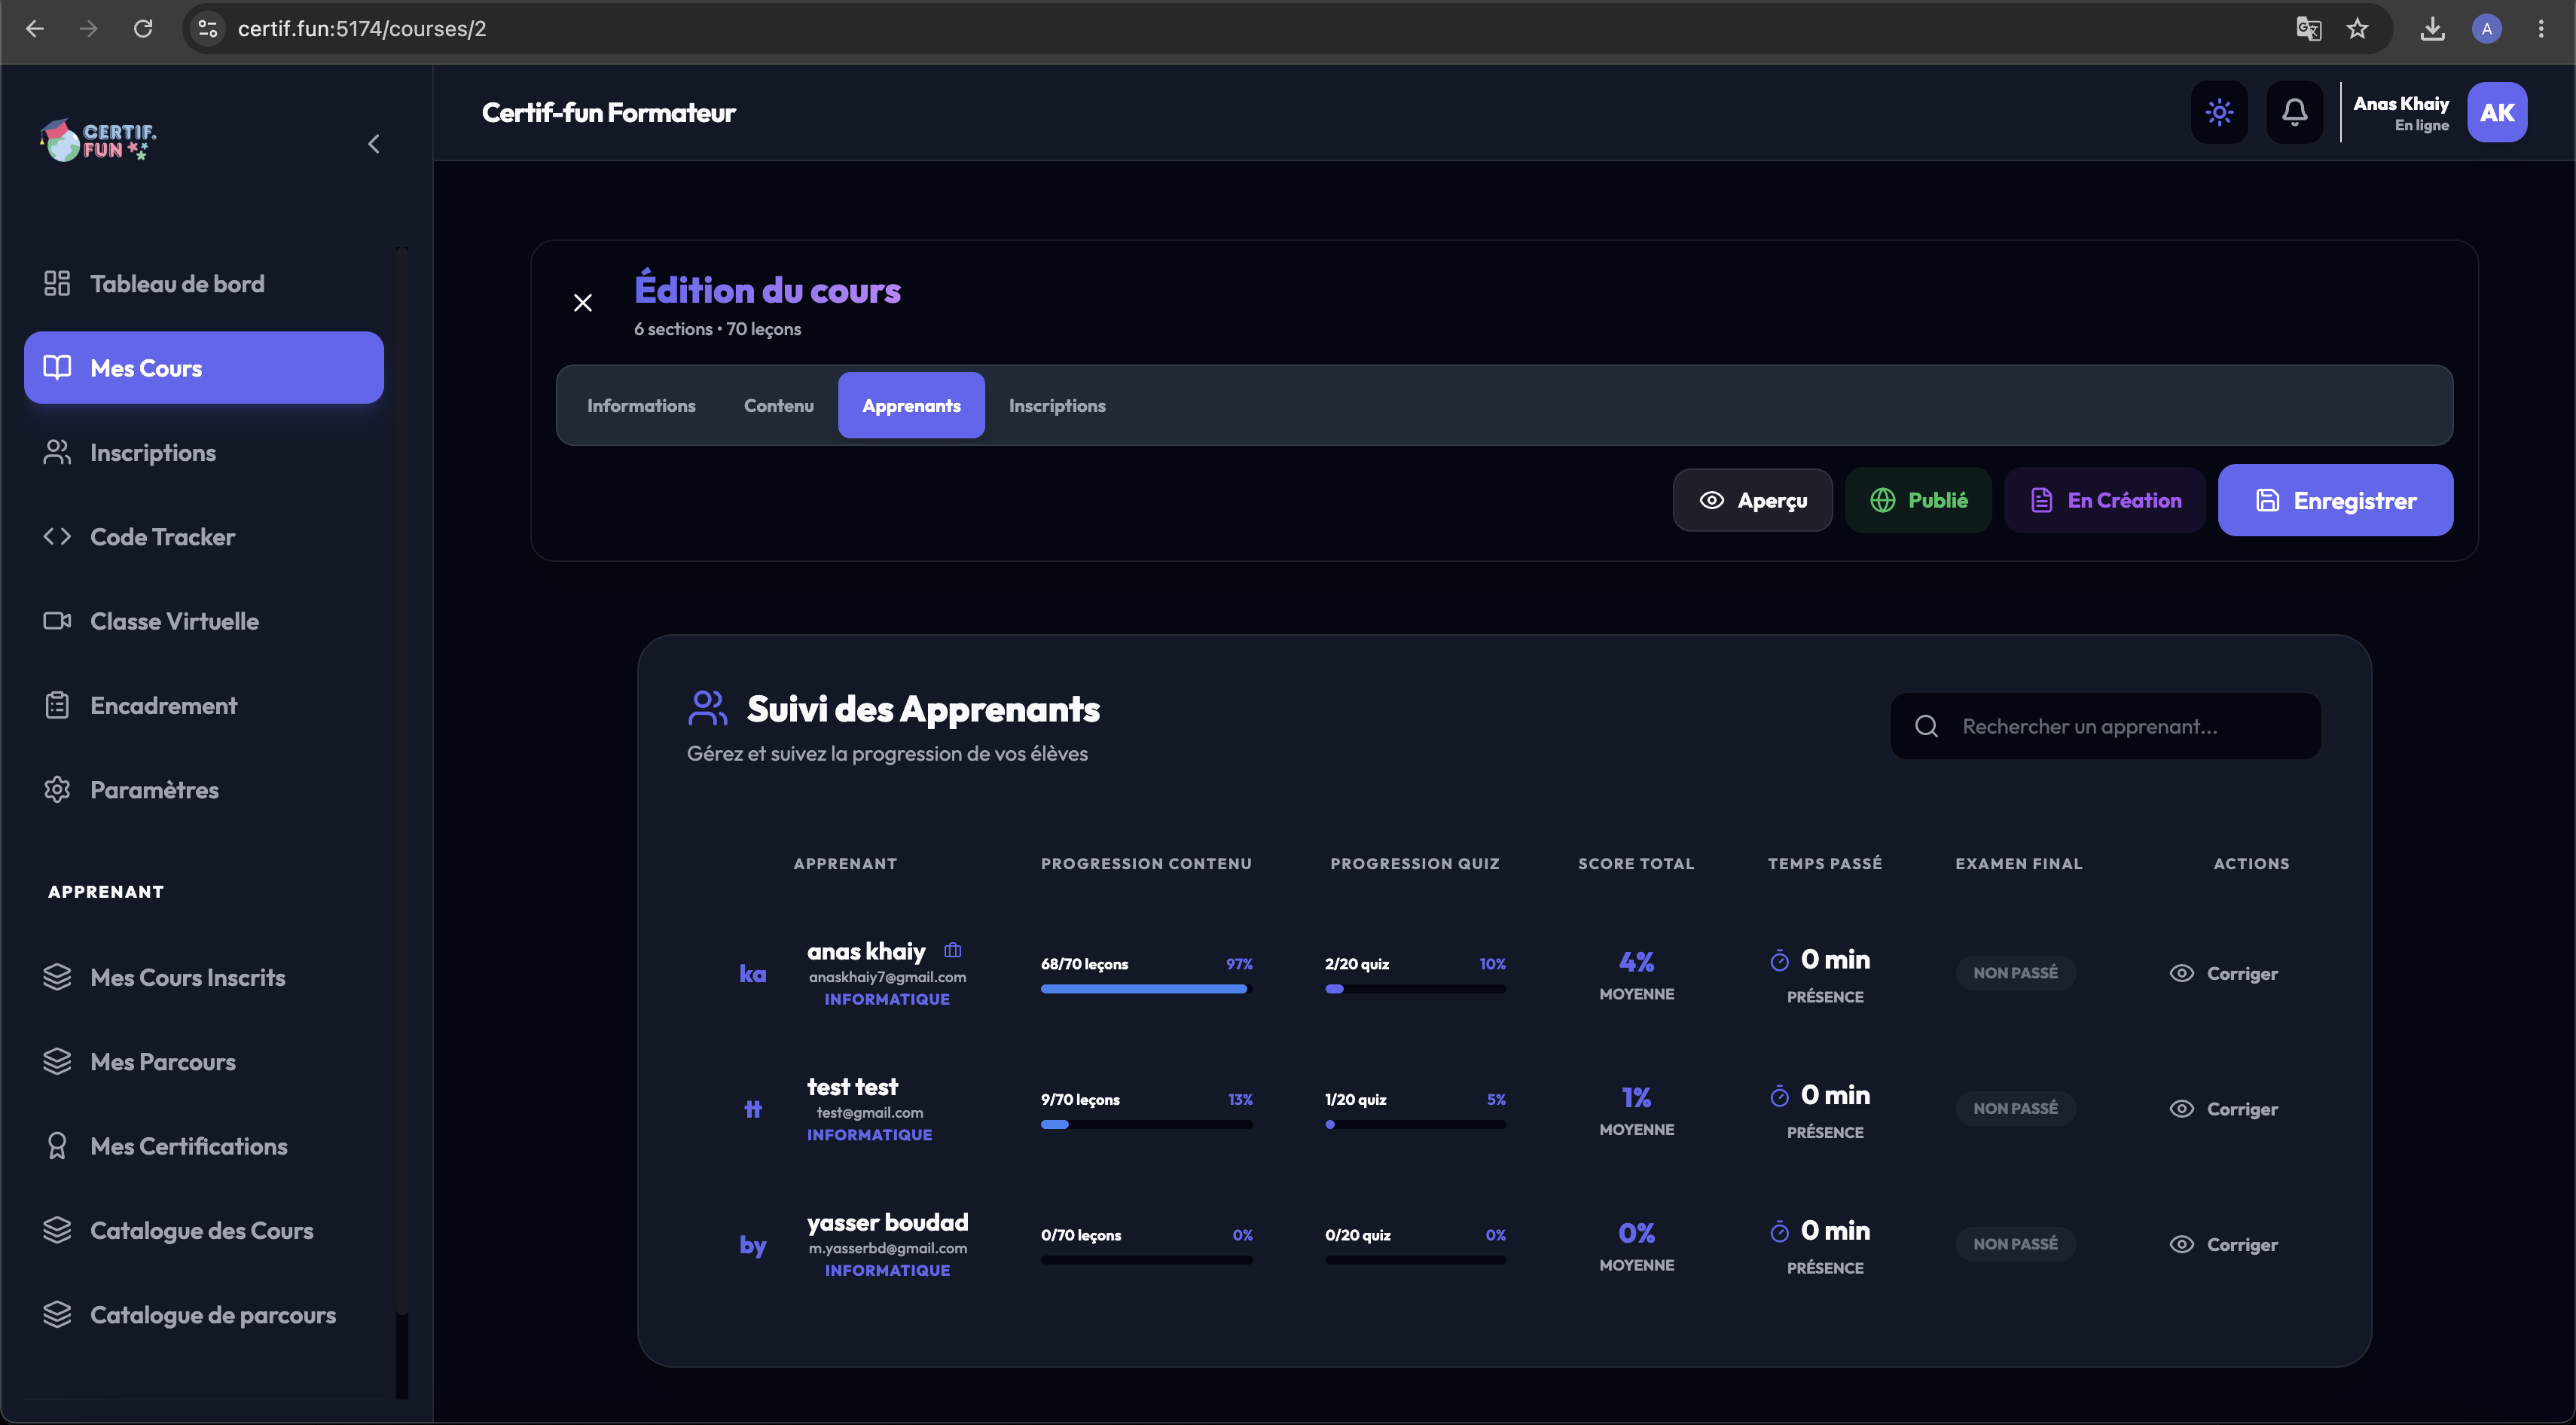
\includegraphics[width=0.98\textwidth]{figures/formateur-4.png}
    \caption{Éditeur de contenu du cours}
    \label{fig:formateur4}
\end{figure}

Le module des inscriptions (Figure~\ref{fig:formateur5}) permet au formateur de gérer directement les inscriptions et les accès de ses apprenants à ses cours.
\begin{figure}[H]
    \centering
    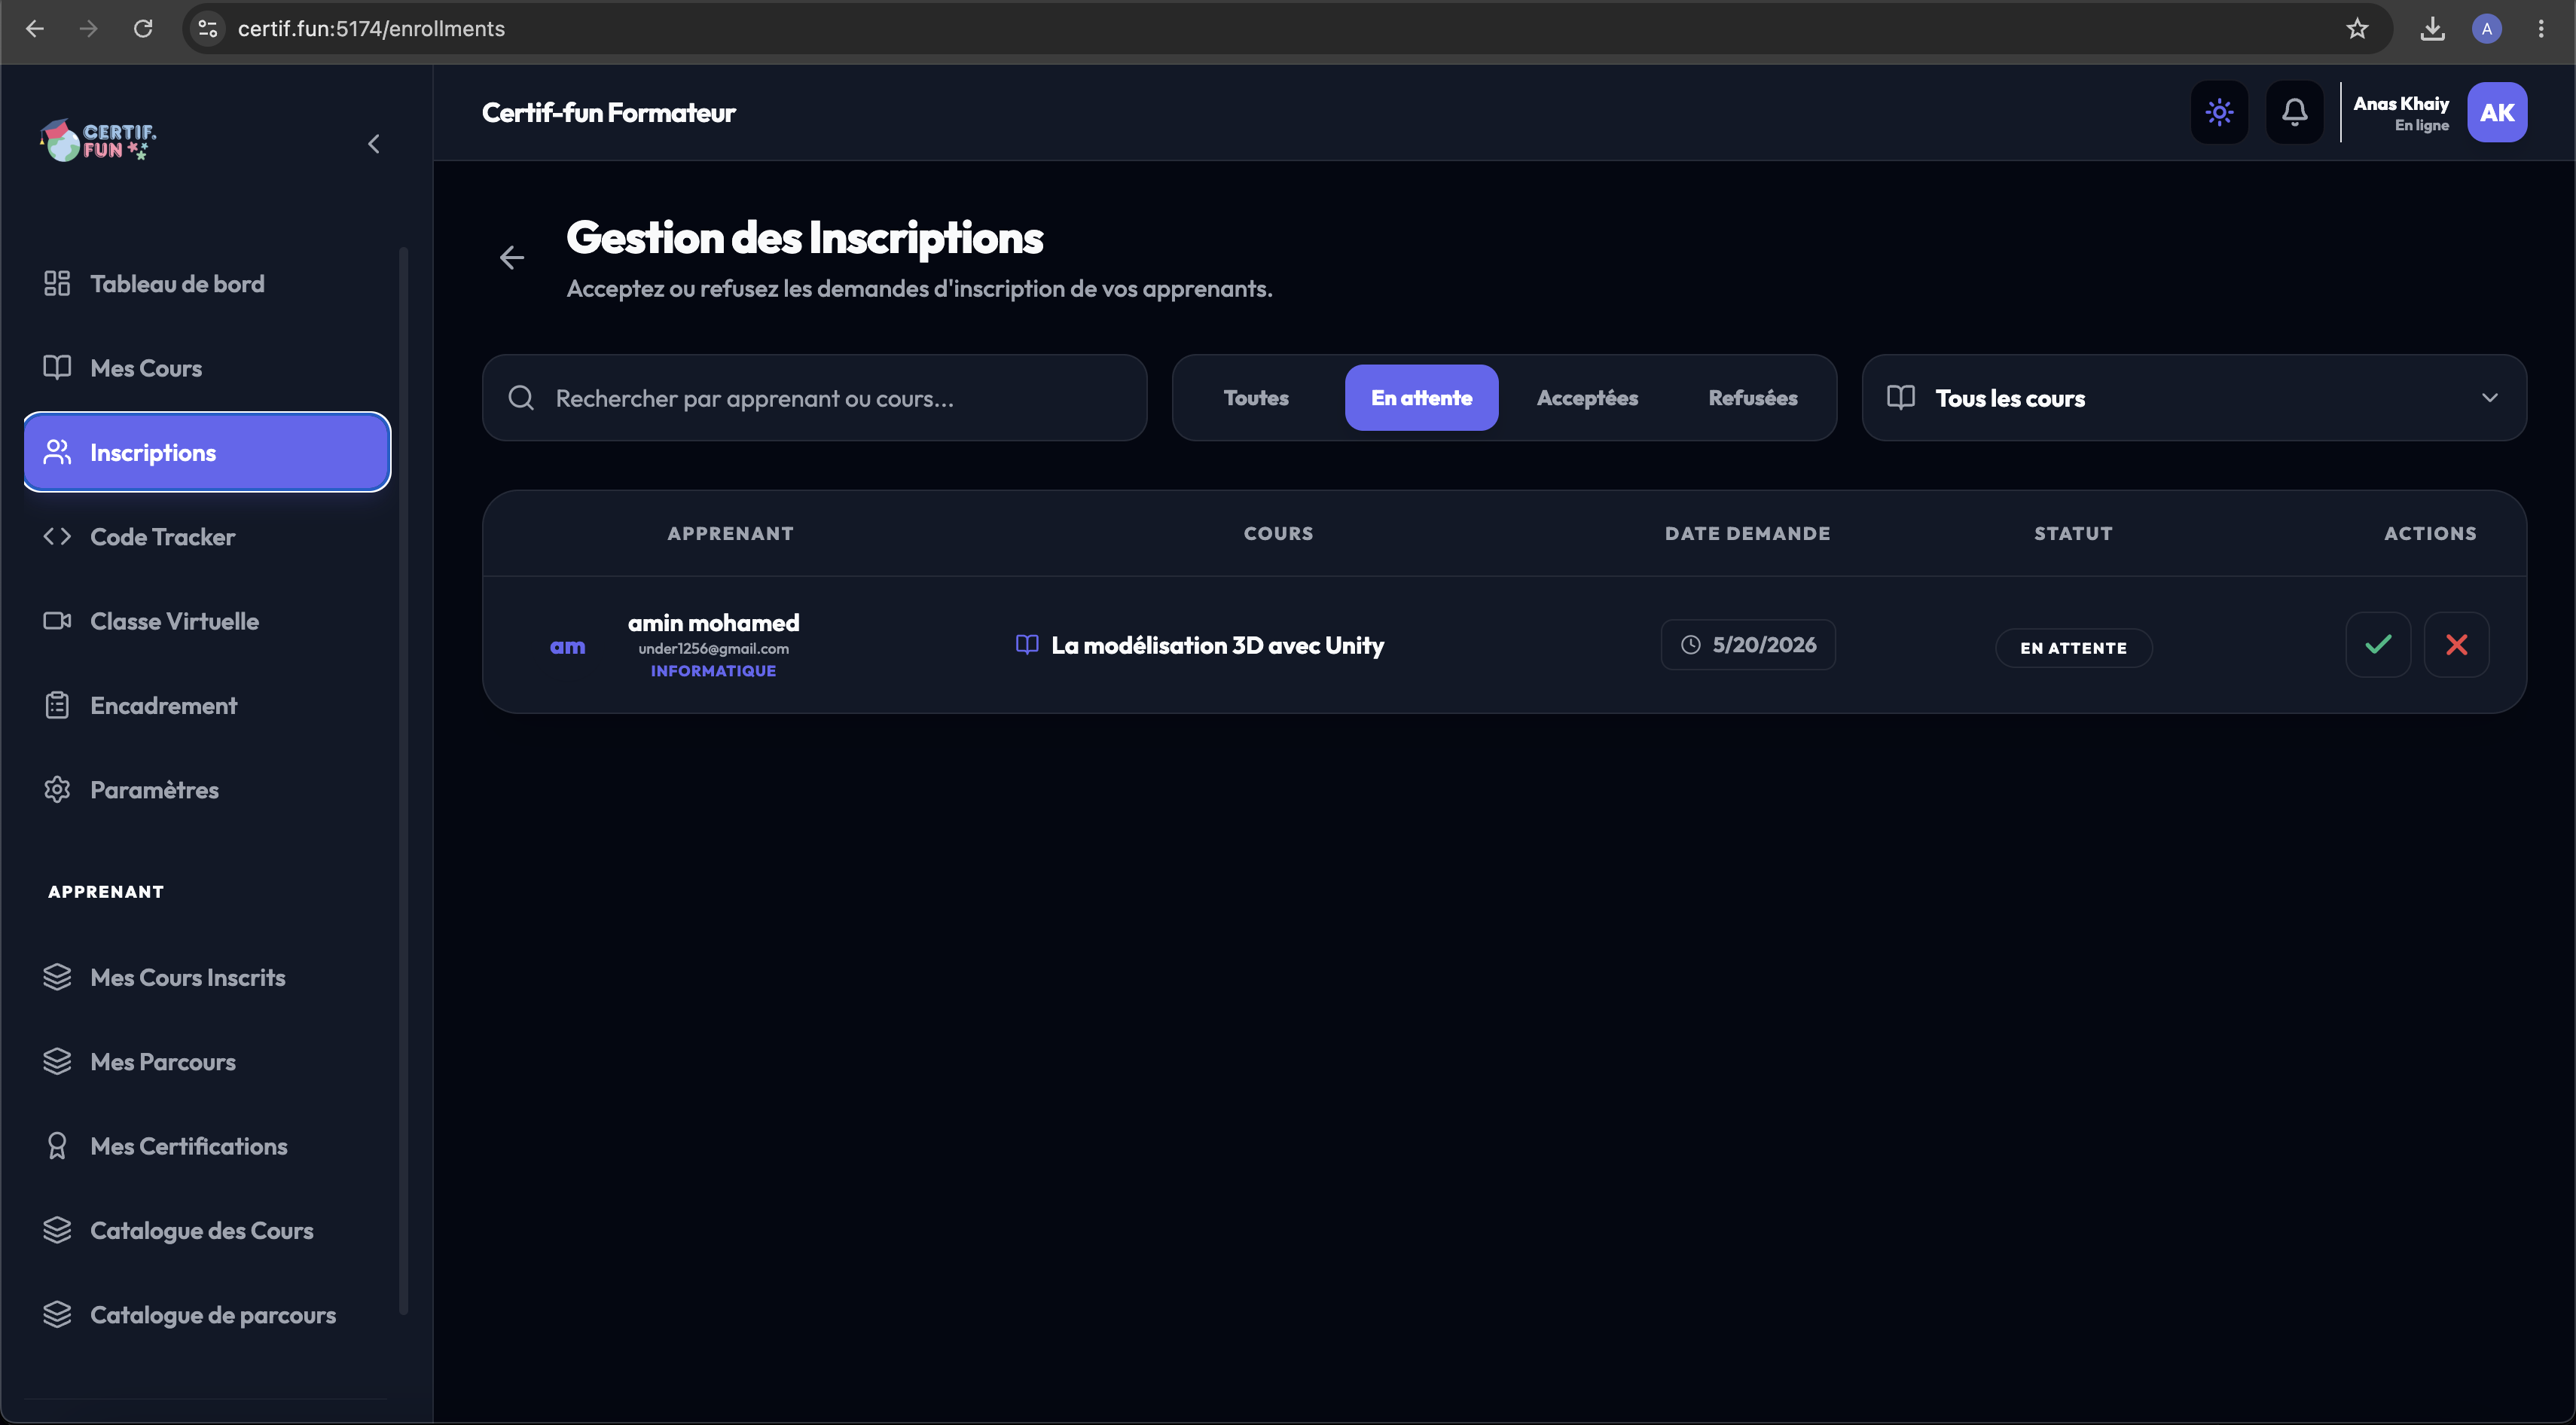
\includegraphics[width=0.98\textwidth]{figures/formateur-5.png}
    \caption{Suivi des inscriptions aux cours du formateur}
    \label{fig:formateur5}
\end{figure}

Pour les matières liées à la programmation, l'outil "Code Tracker" (Figure~\ref{fig:formateur6}) donne la possibilité au formateur de consulter en direct le code écrit par ses étudiants dans les exercices pratiques.
\begin{figure}[H]
    \centering
    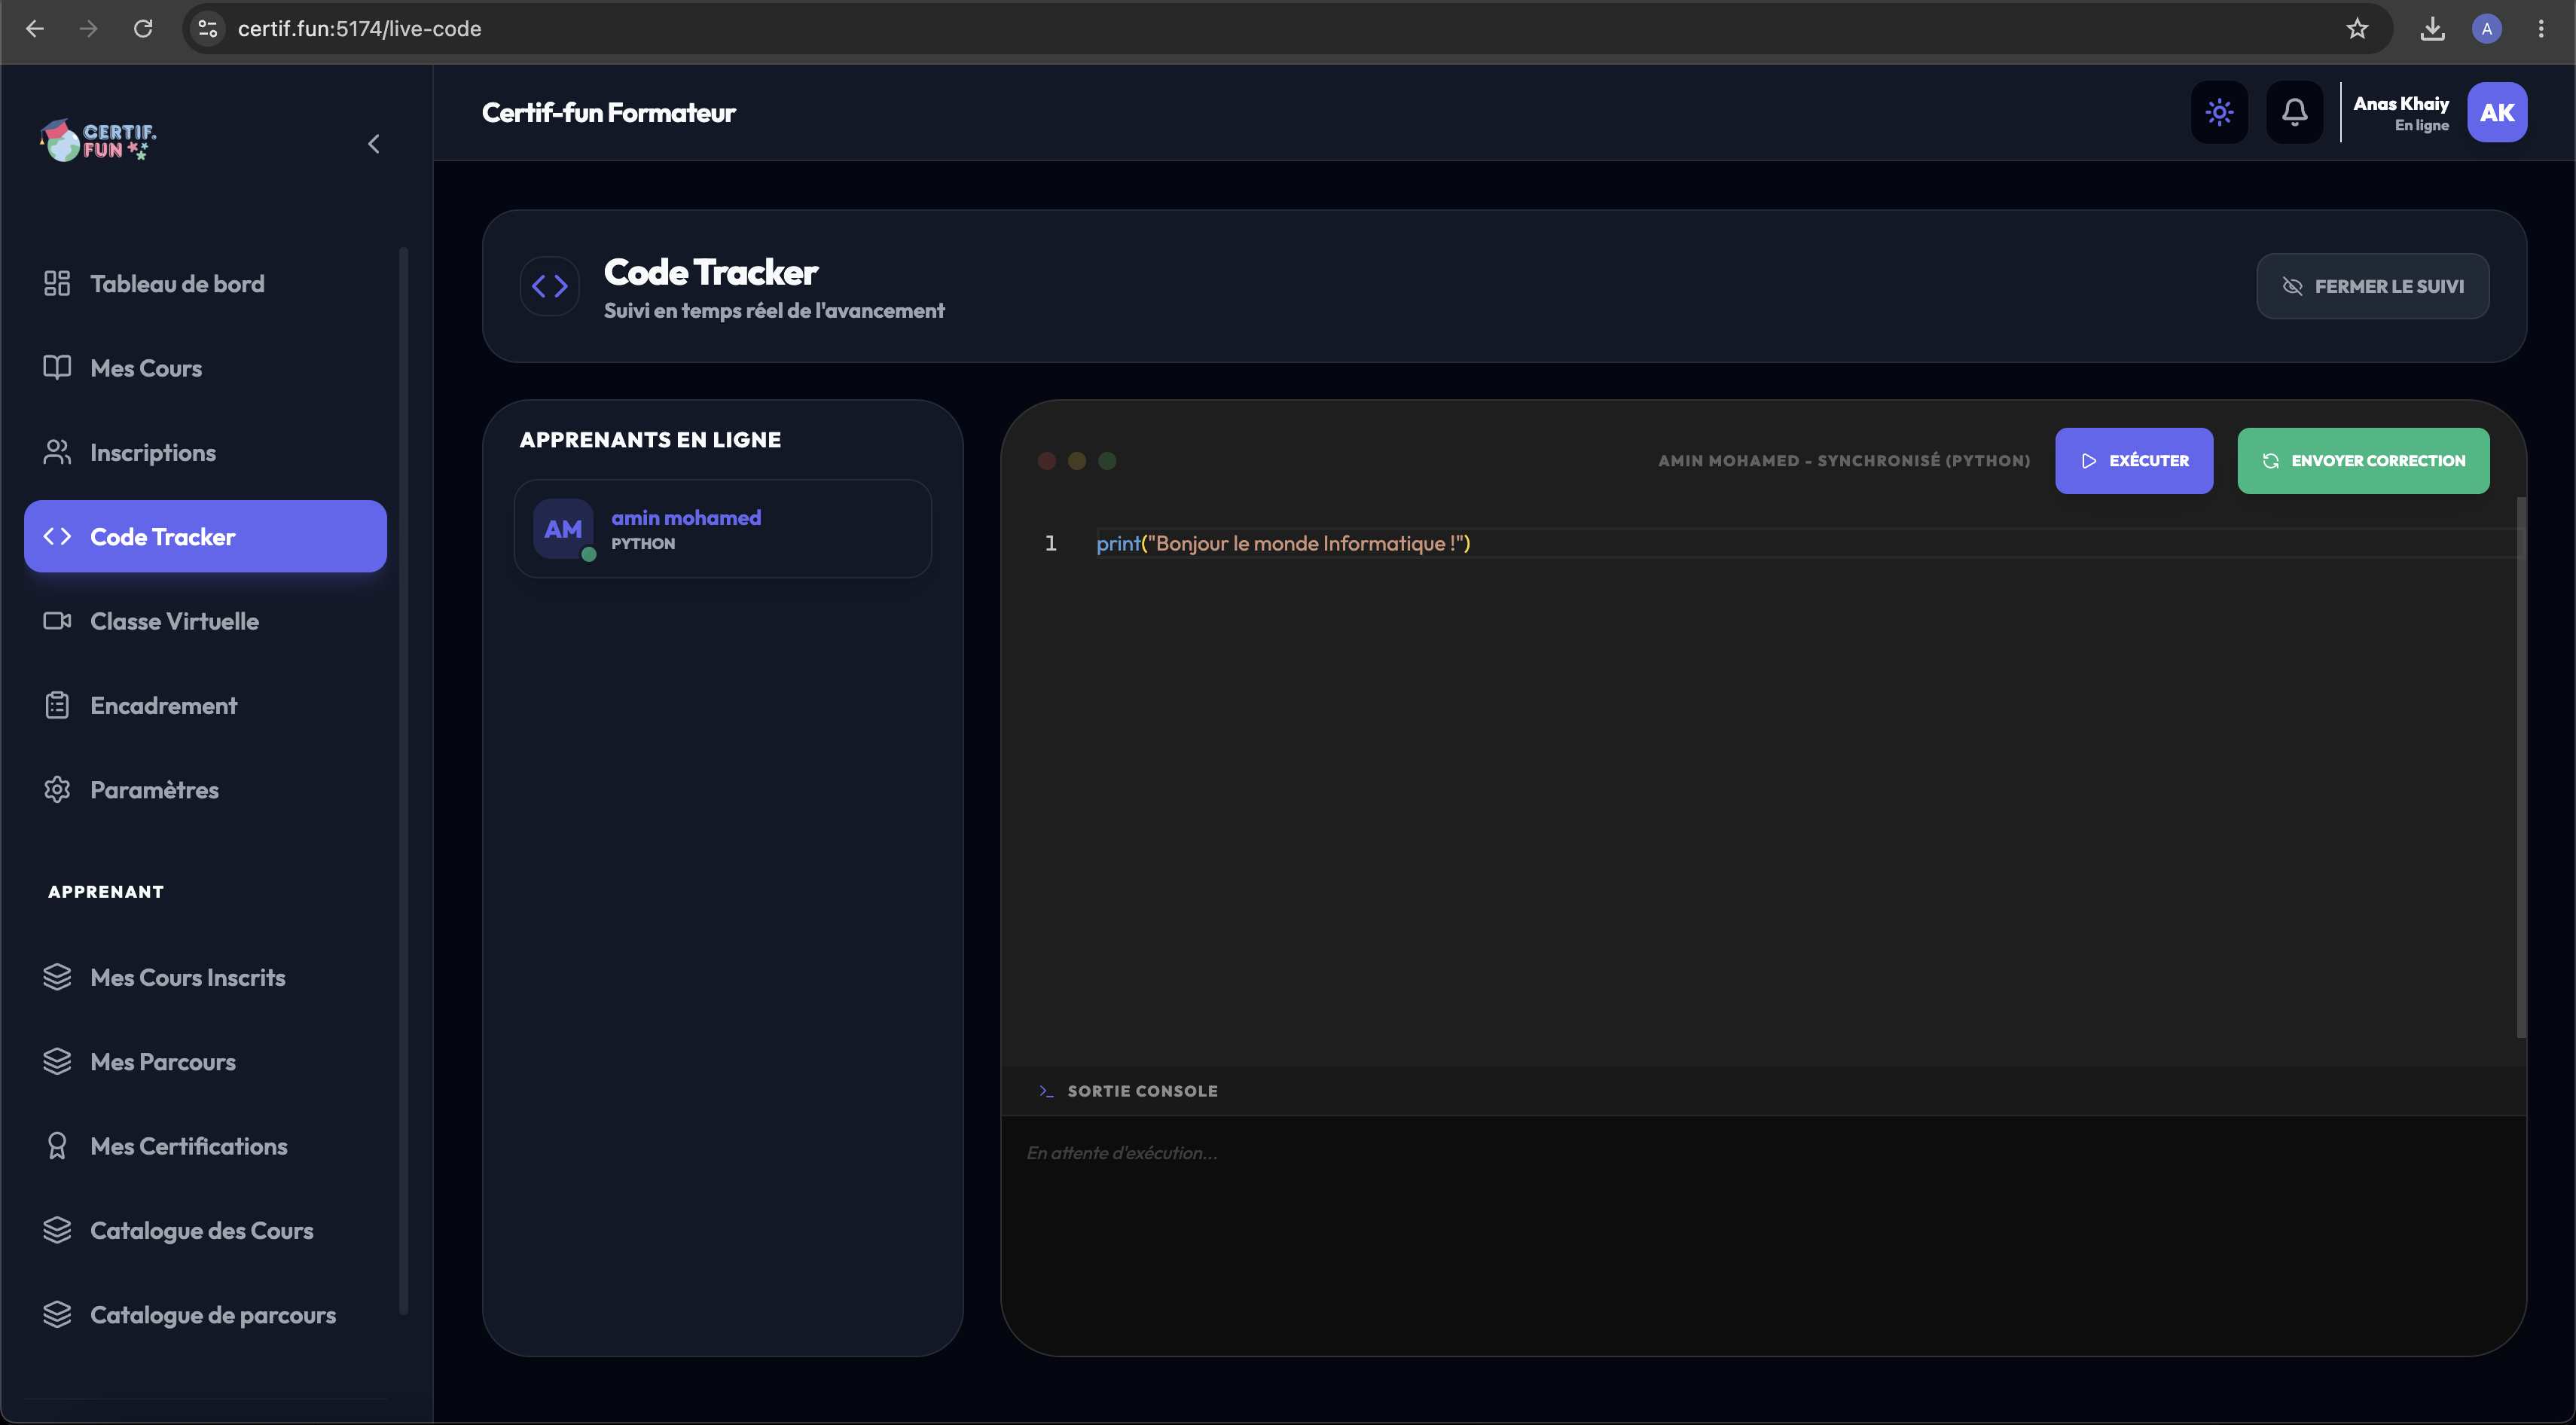
\includegraphics[width=0.98\textwidth]{figures/formateur-6.png}
    \caption{Outil Code Tracker pour les exercices de programmation}
    \label{fig:formateur6}
\end{figure}

Le module "Classe Virtuelle" (Figure~\ref{fig:formateur7}) permet au professeur d'initier une session d'enseignement en visioconférence. Il génère un code de salle (ex. ROOM-EN4SBU1E) qu'il transmet à ses apprenants pour un cours en direct avec partage d'écran et audio.
\begin{figure}[H]
    \centering
    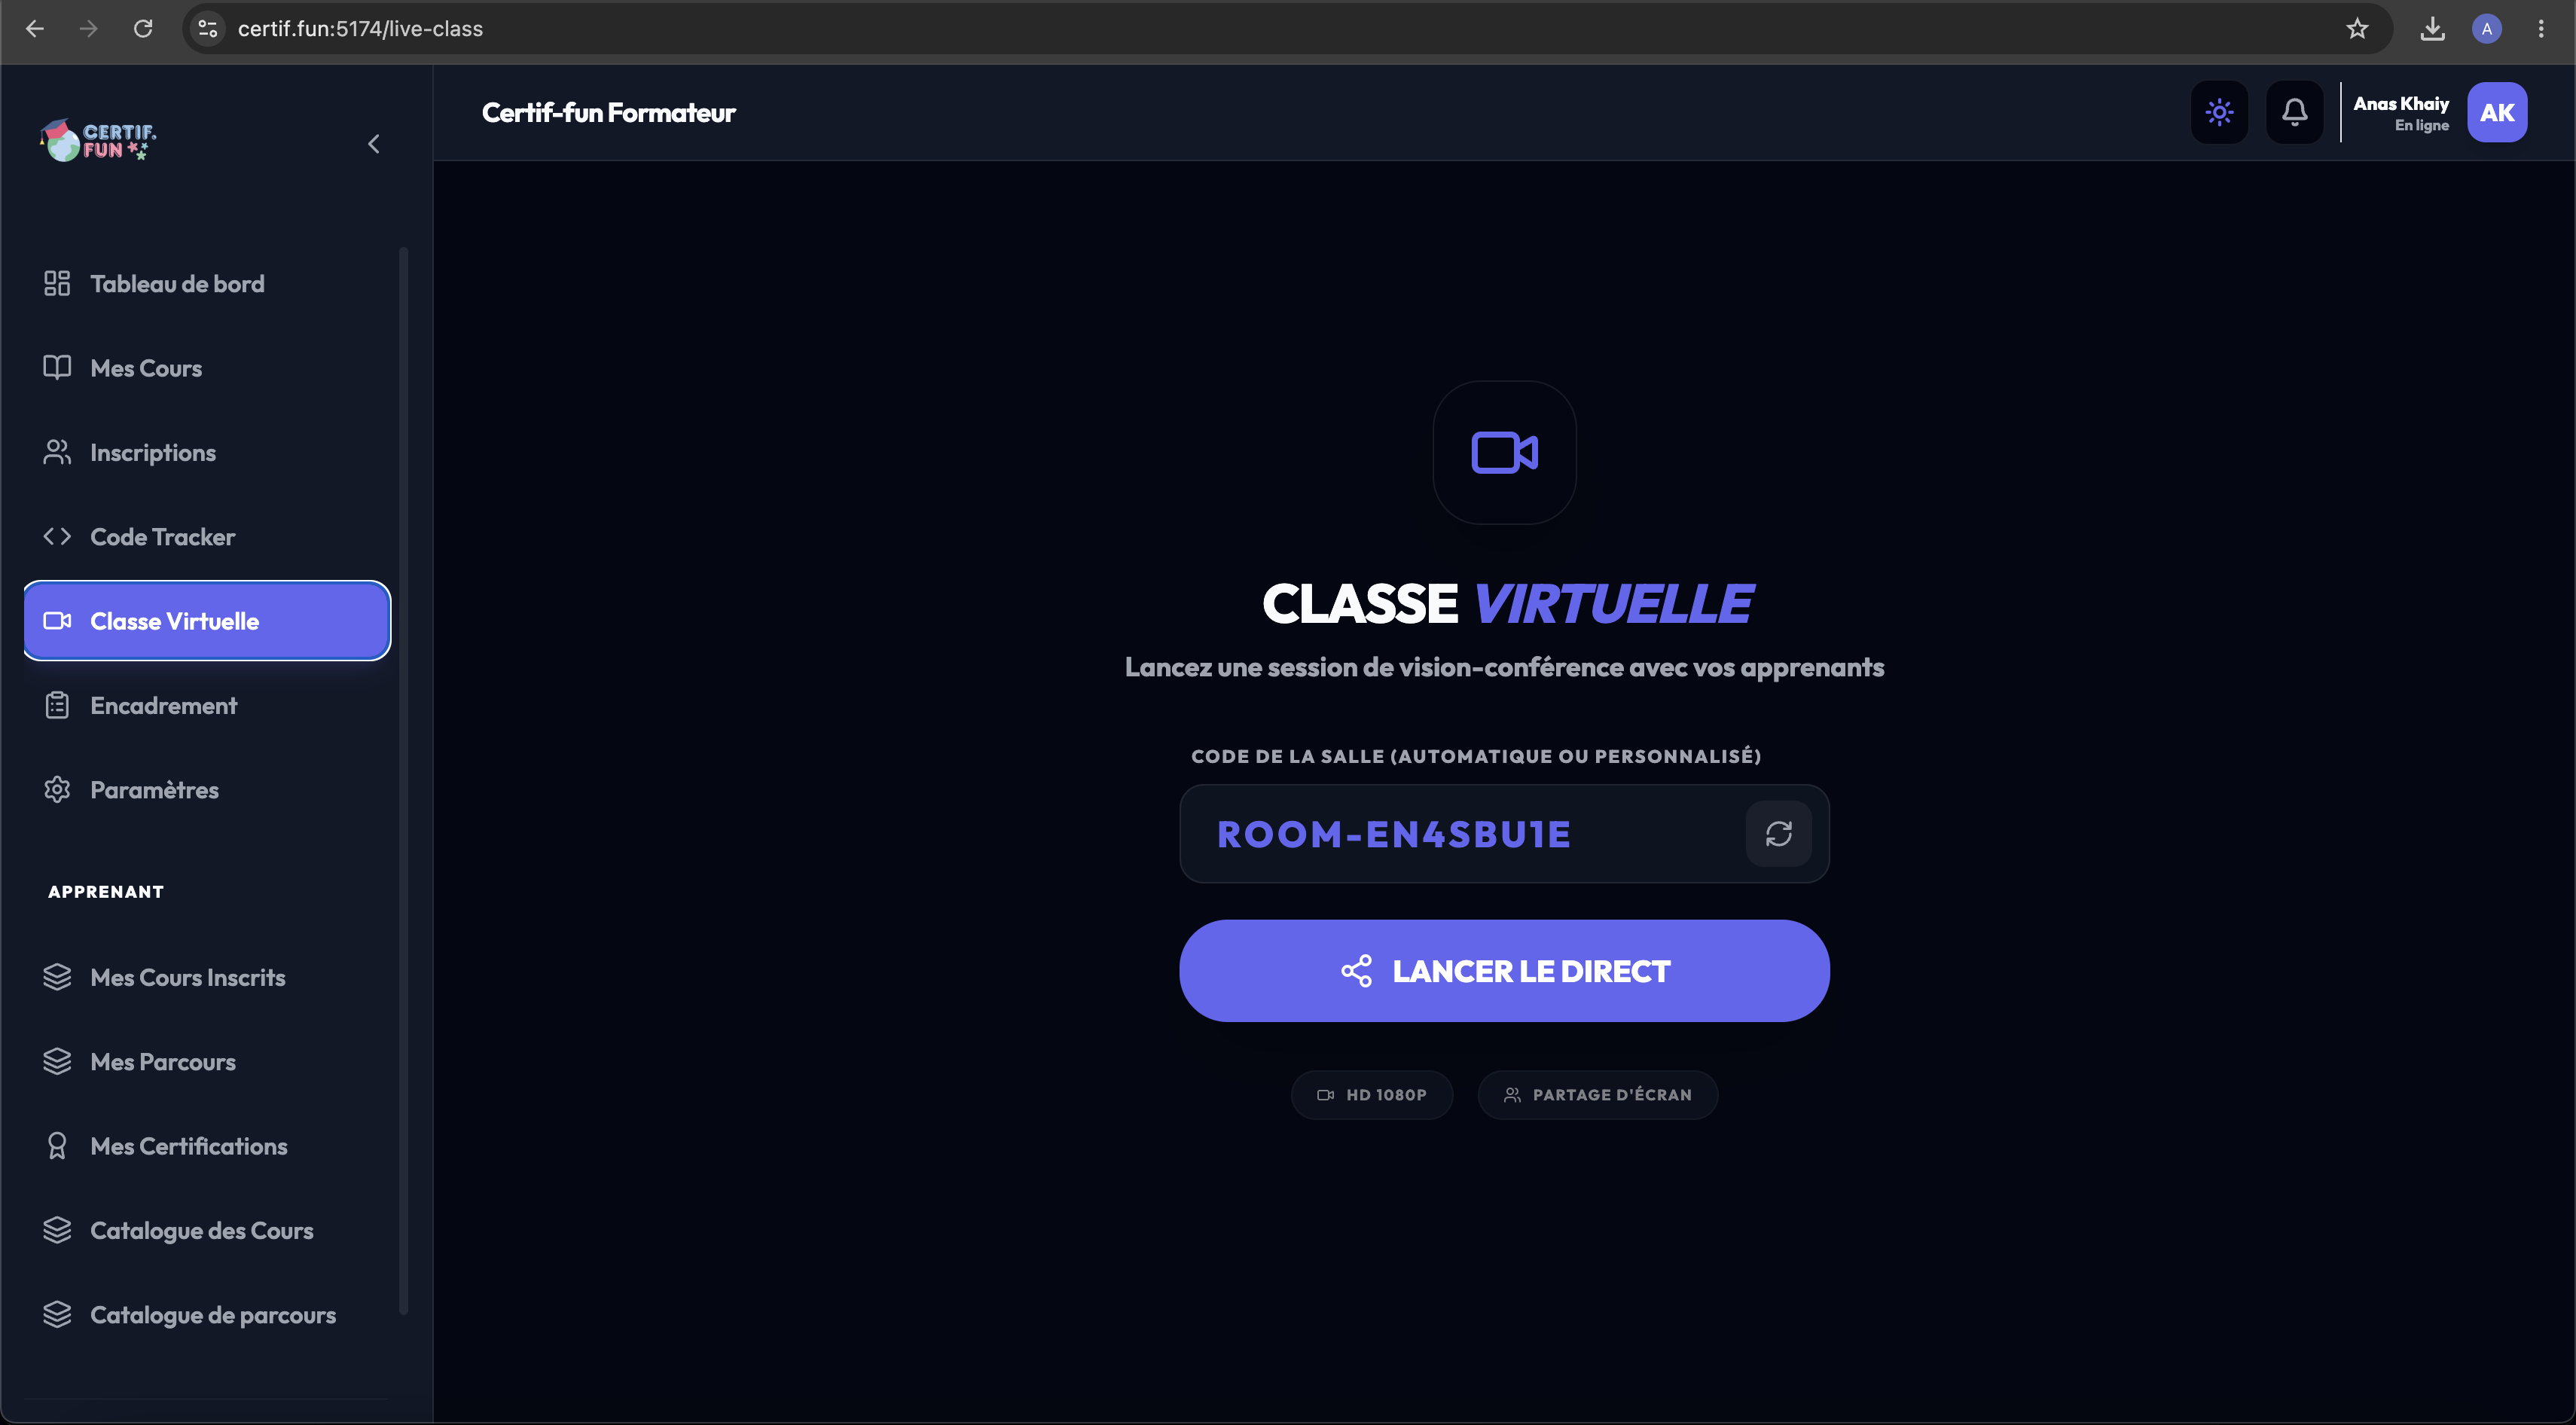
\includegraphics[width=0.98\textwidth]{figures/formateur-7.png}
    \caption{Interface de lancement d'une classe virtuelle}
    \label{fig:formateur7}
\end{figure}

La section "Mon Encadrement" (Figure~\ref{fig:formateur8}) est dédiée au suivi des PFE et des projets longs. Le formateur y suit l'avancement individuel de chaque apprenant encadré et valide ses livrables (rapports, code).
\begin{figure}[H]
    \centering
    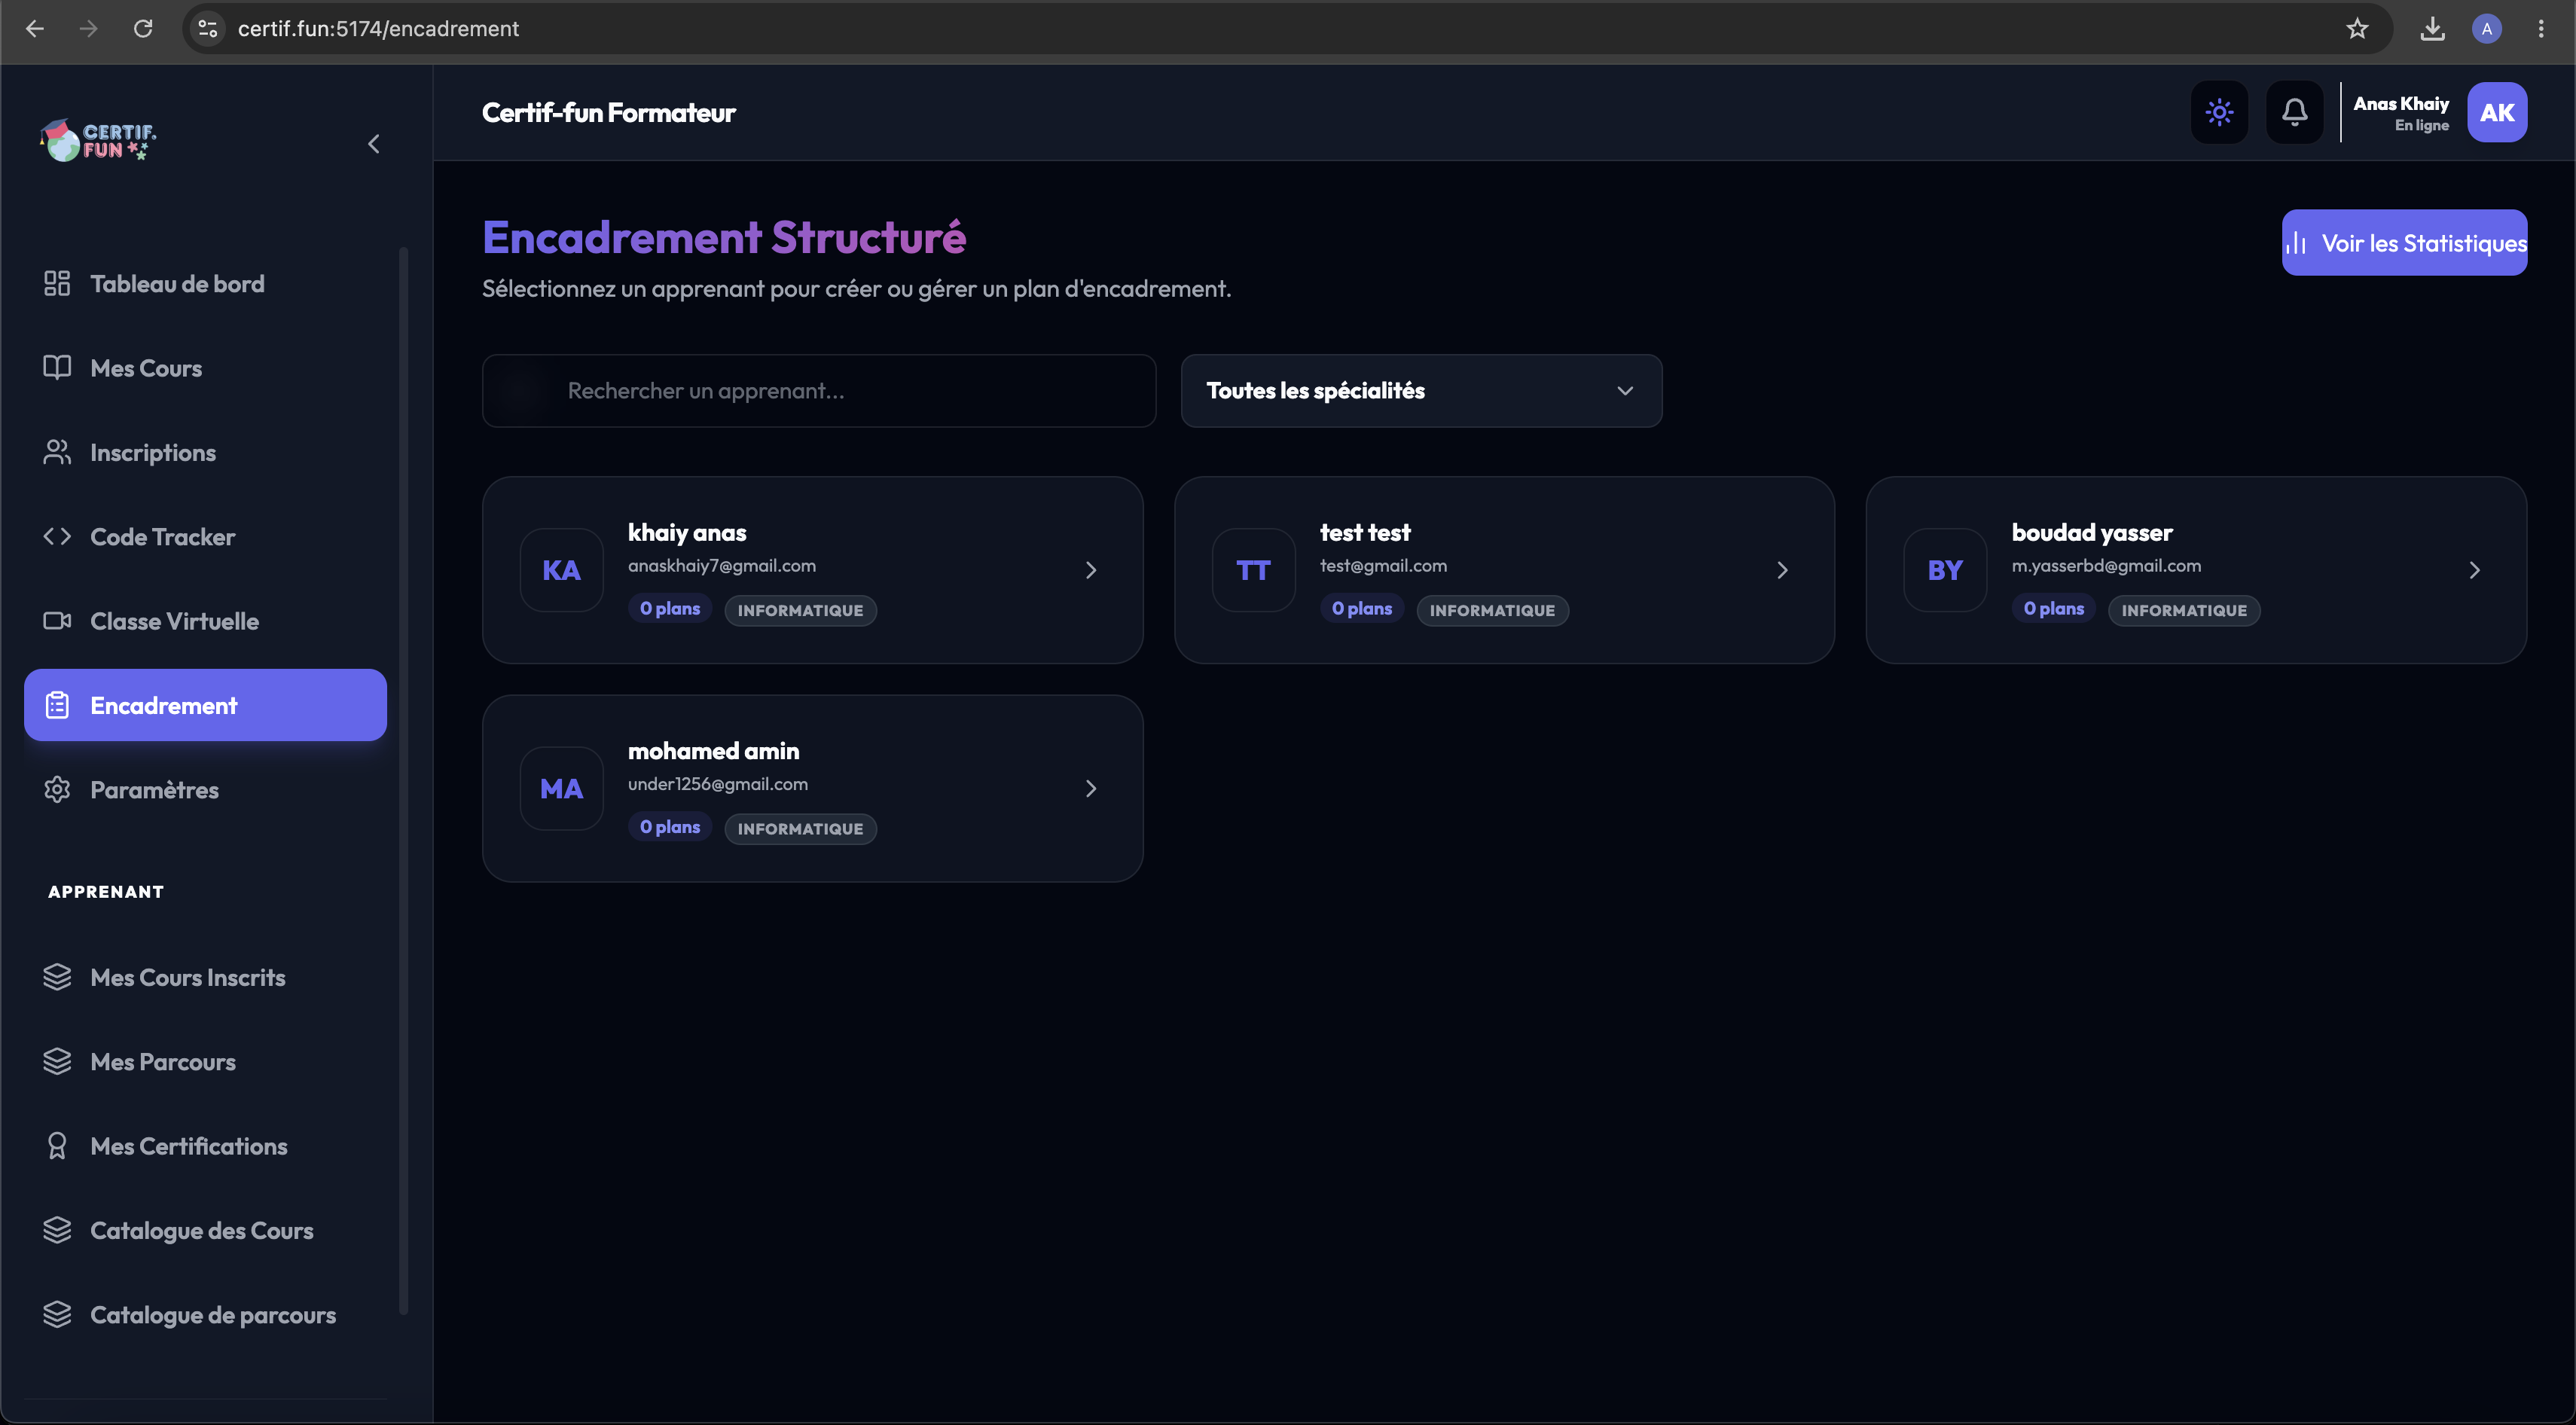
\includegraphics[width=0.98\textwidth]{figures/formateur-8.png}
    \caption{Tableau de bord de l'encadrement structuré}
    \label{fig:formateur8}
\end{figure}

Enfin, le formateur a accès au catalogue des parcours (Figure~\ref{fig:formateur9}), ce qui lui permet de consulter des parcours contenant plusieurs cours afin de se perfectionner via des master classes.
\begin{figure}[H]
    \centering
    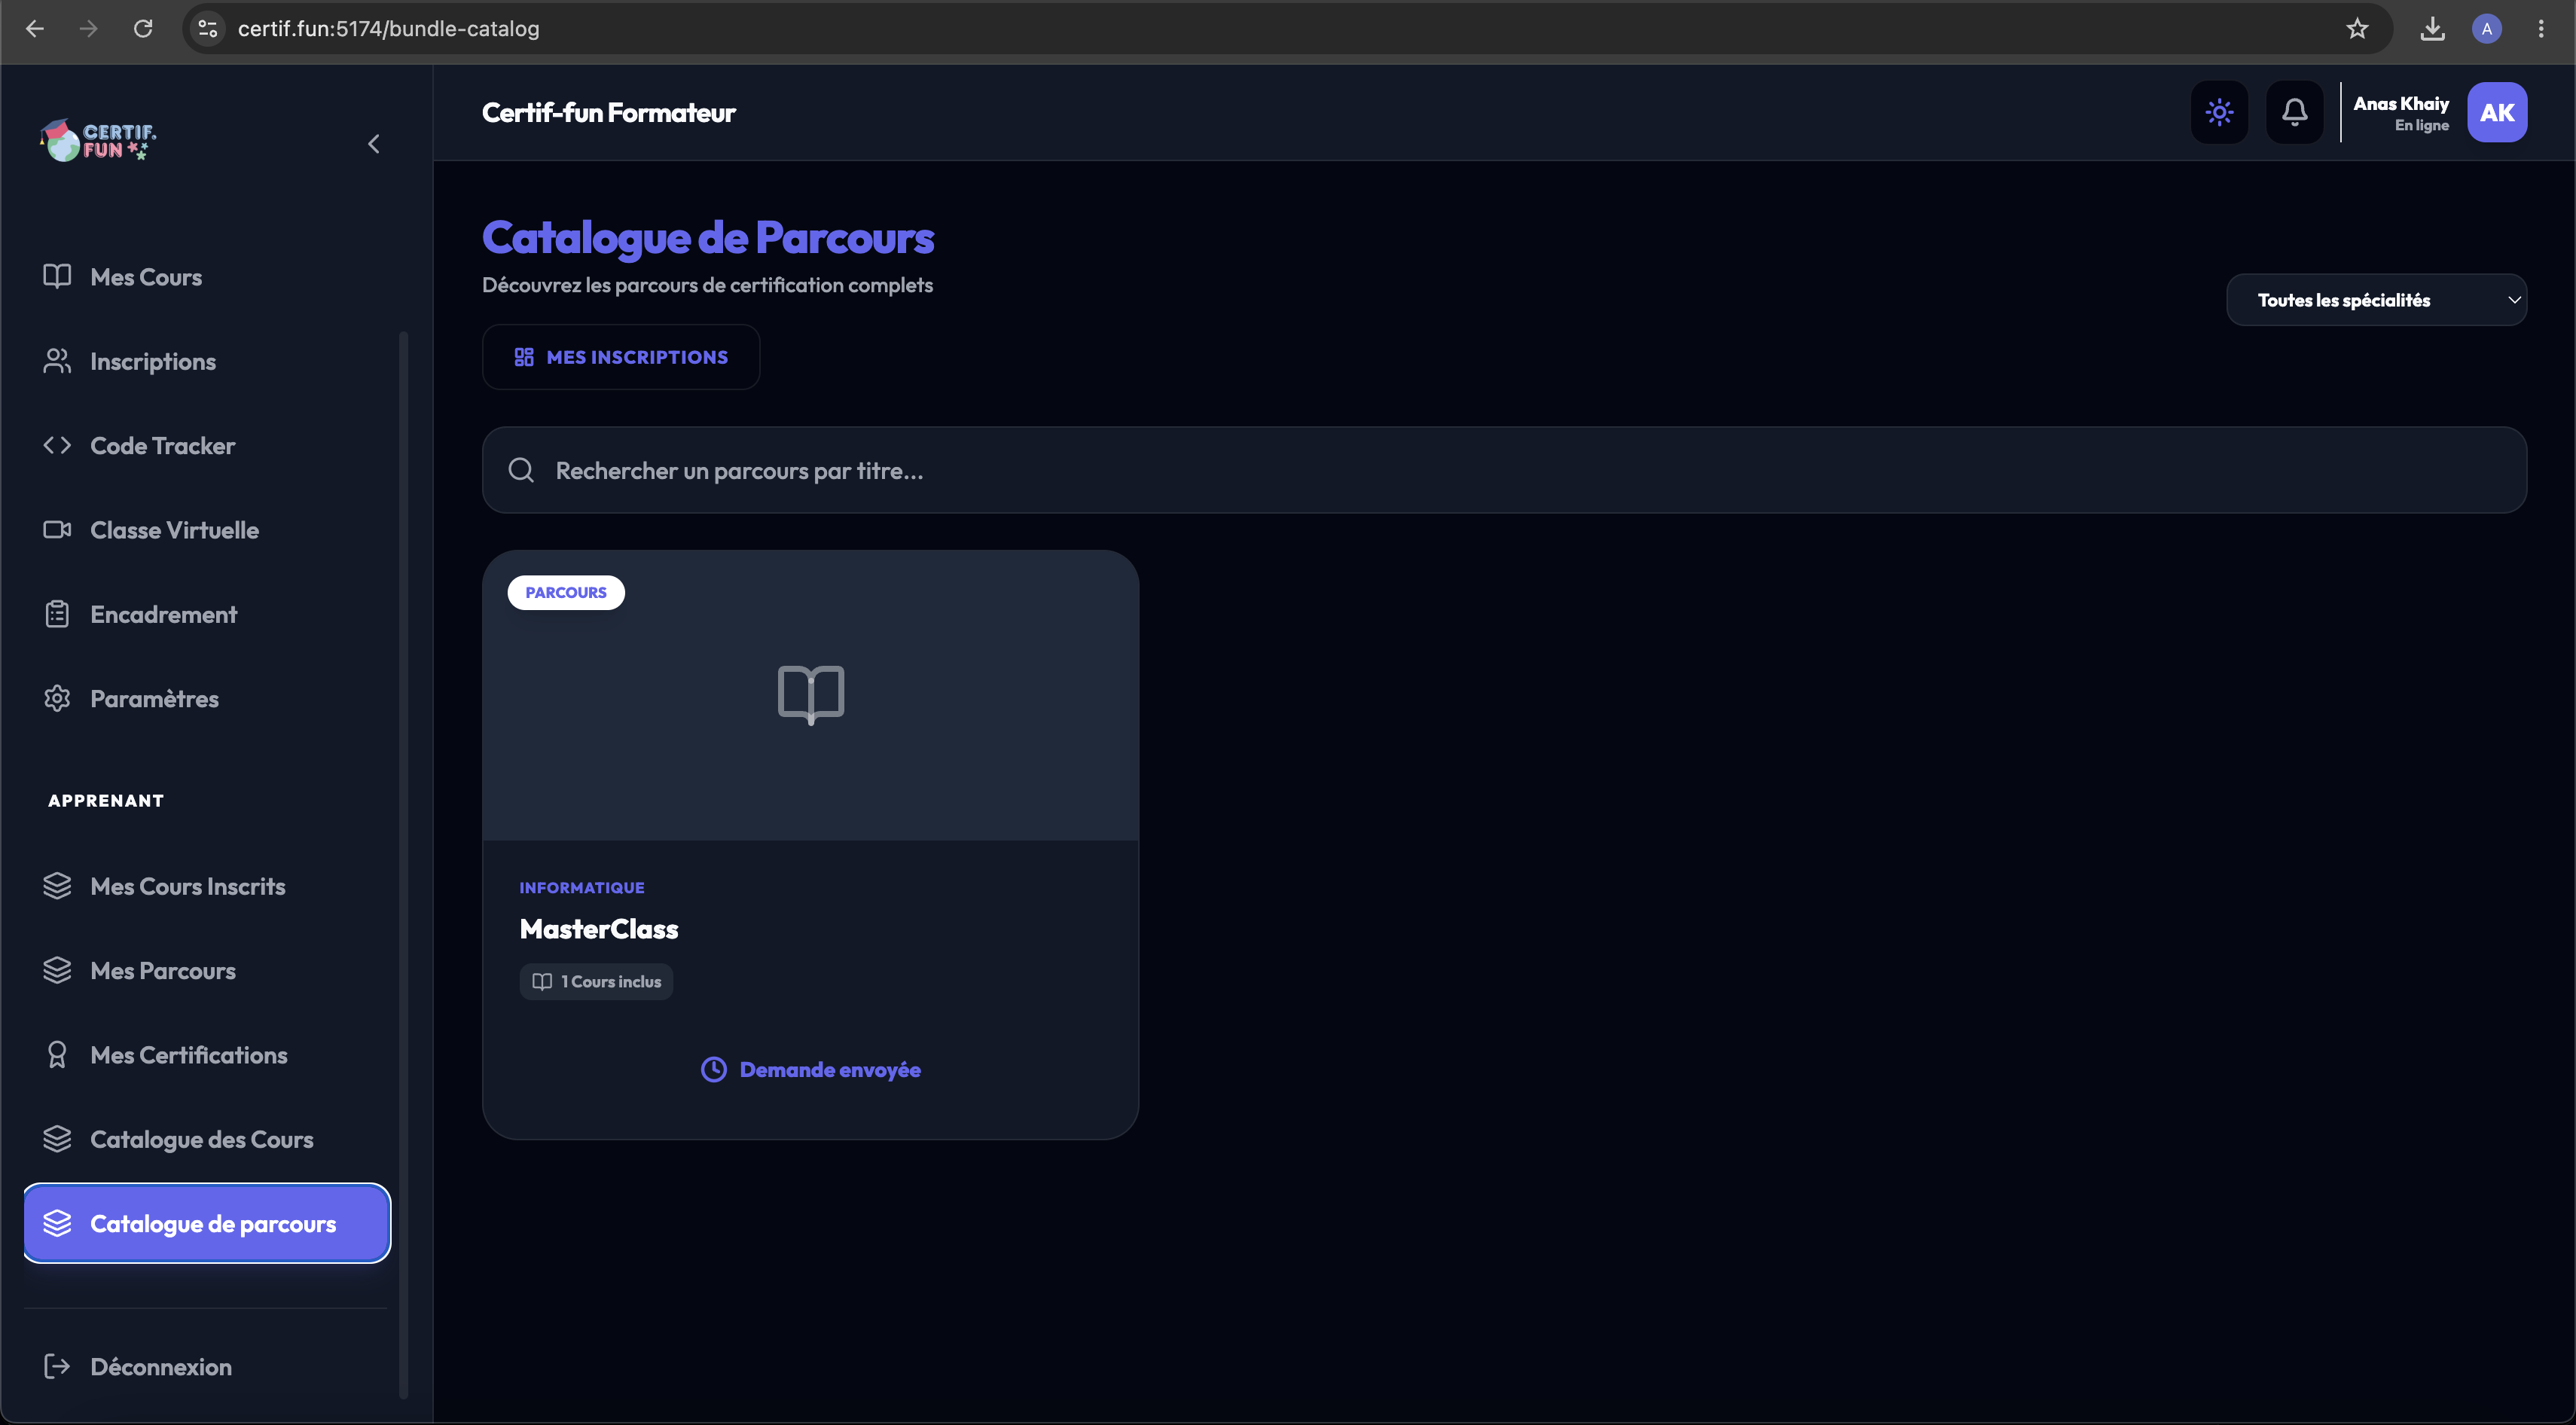
\includegraphics[width=0.98\textwidth]{figures/formateur-9.png}
    \caption{Catalogue global des parcours de certification}
    \label{fig:formateur9}
\end{figure}

Le module de configuration de l'examen final (Figure~\ref{fig:formateur10}) permet au formateur de définir la structure du quiz. Le pool de questions est généré à partir de la masse horaire pour chaque section. Il peut configurer chaque chapitre (section) en spécifiant le poids en pourcentage et le nombre de questions à tirer aléatoirement parmi celles disponibles. Le bilan total affiche le nombre total de questions sélectionnées.
\begin{figure}[H]
    \centering
    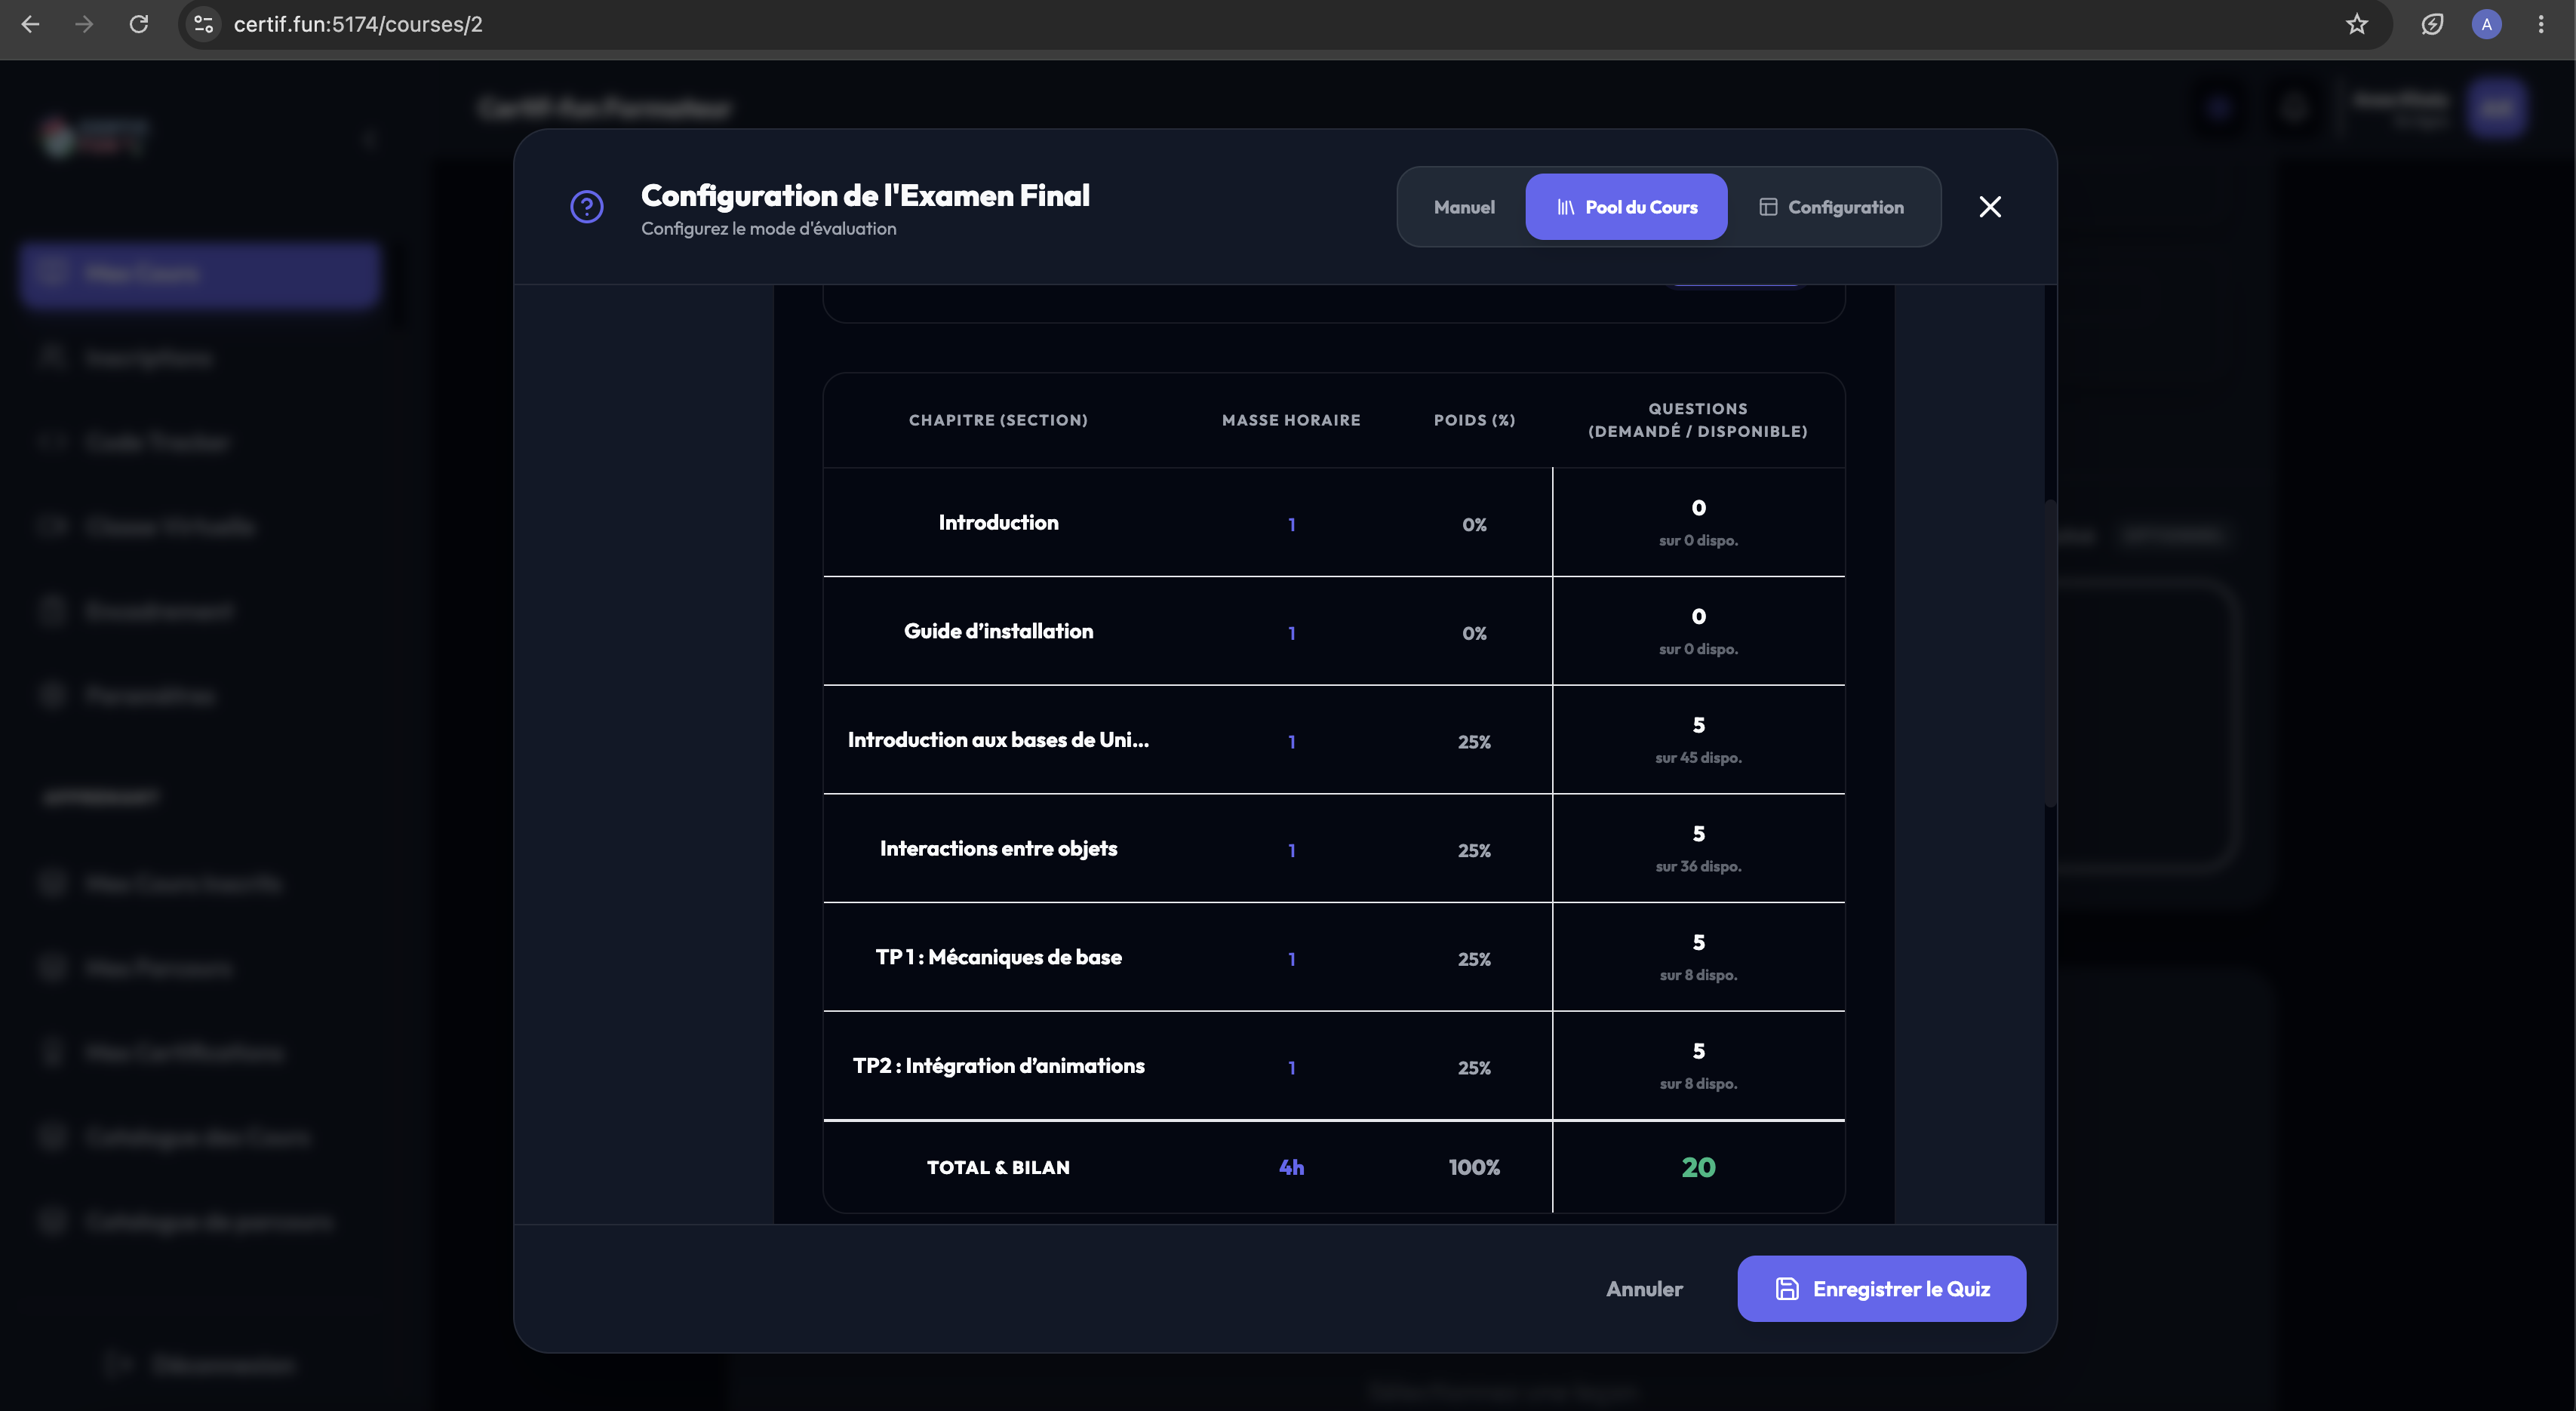
\includegraphics[width=0.98\textwidth]{figures/formateur-10.png}
    \caption{Configuration de l'examen final -- Pool du Cours}
    \label{fig:formateur10}
\end{figure}

La figure~\ref{fig:formateur11} illustre l'onglet de configuration avancée offrant au formateur les contrôles de surveillance par IA (Caméra). Lorsqu'elle est activée, l'apprenant doit obligatoirement utiliser sa caméra pendant l'examen. Le formateur peut activer ou désactiver individuellement les contrôles de détection : détection de téléphone portable, présence de plusieurs personnes, objets interdits (tablettes, écrans) et regard détourné. La section des contrôles anti-triche (Navigateur) permet également de détecter les changements d'onglet pendant l'examen.
\begin{figure}[H]
    \centering
    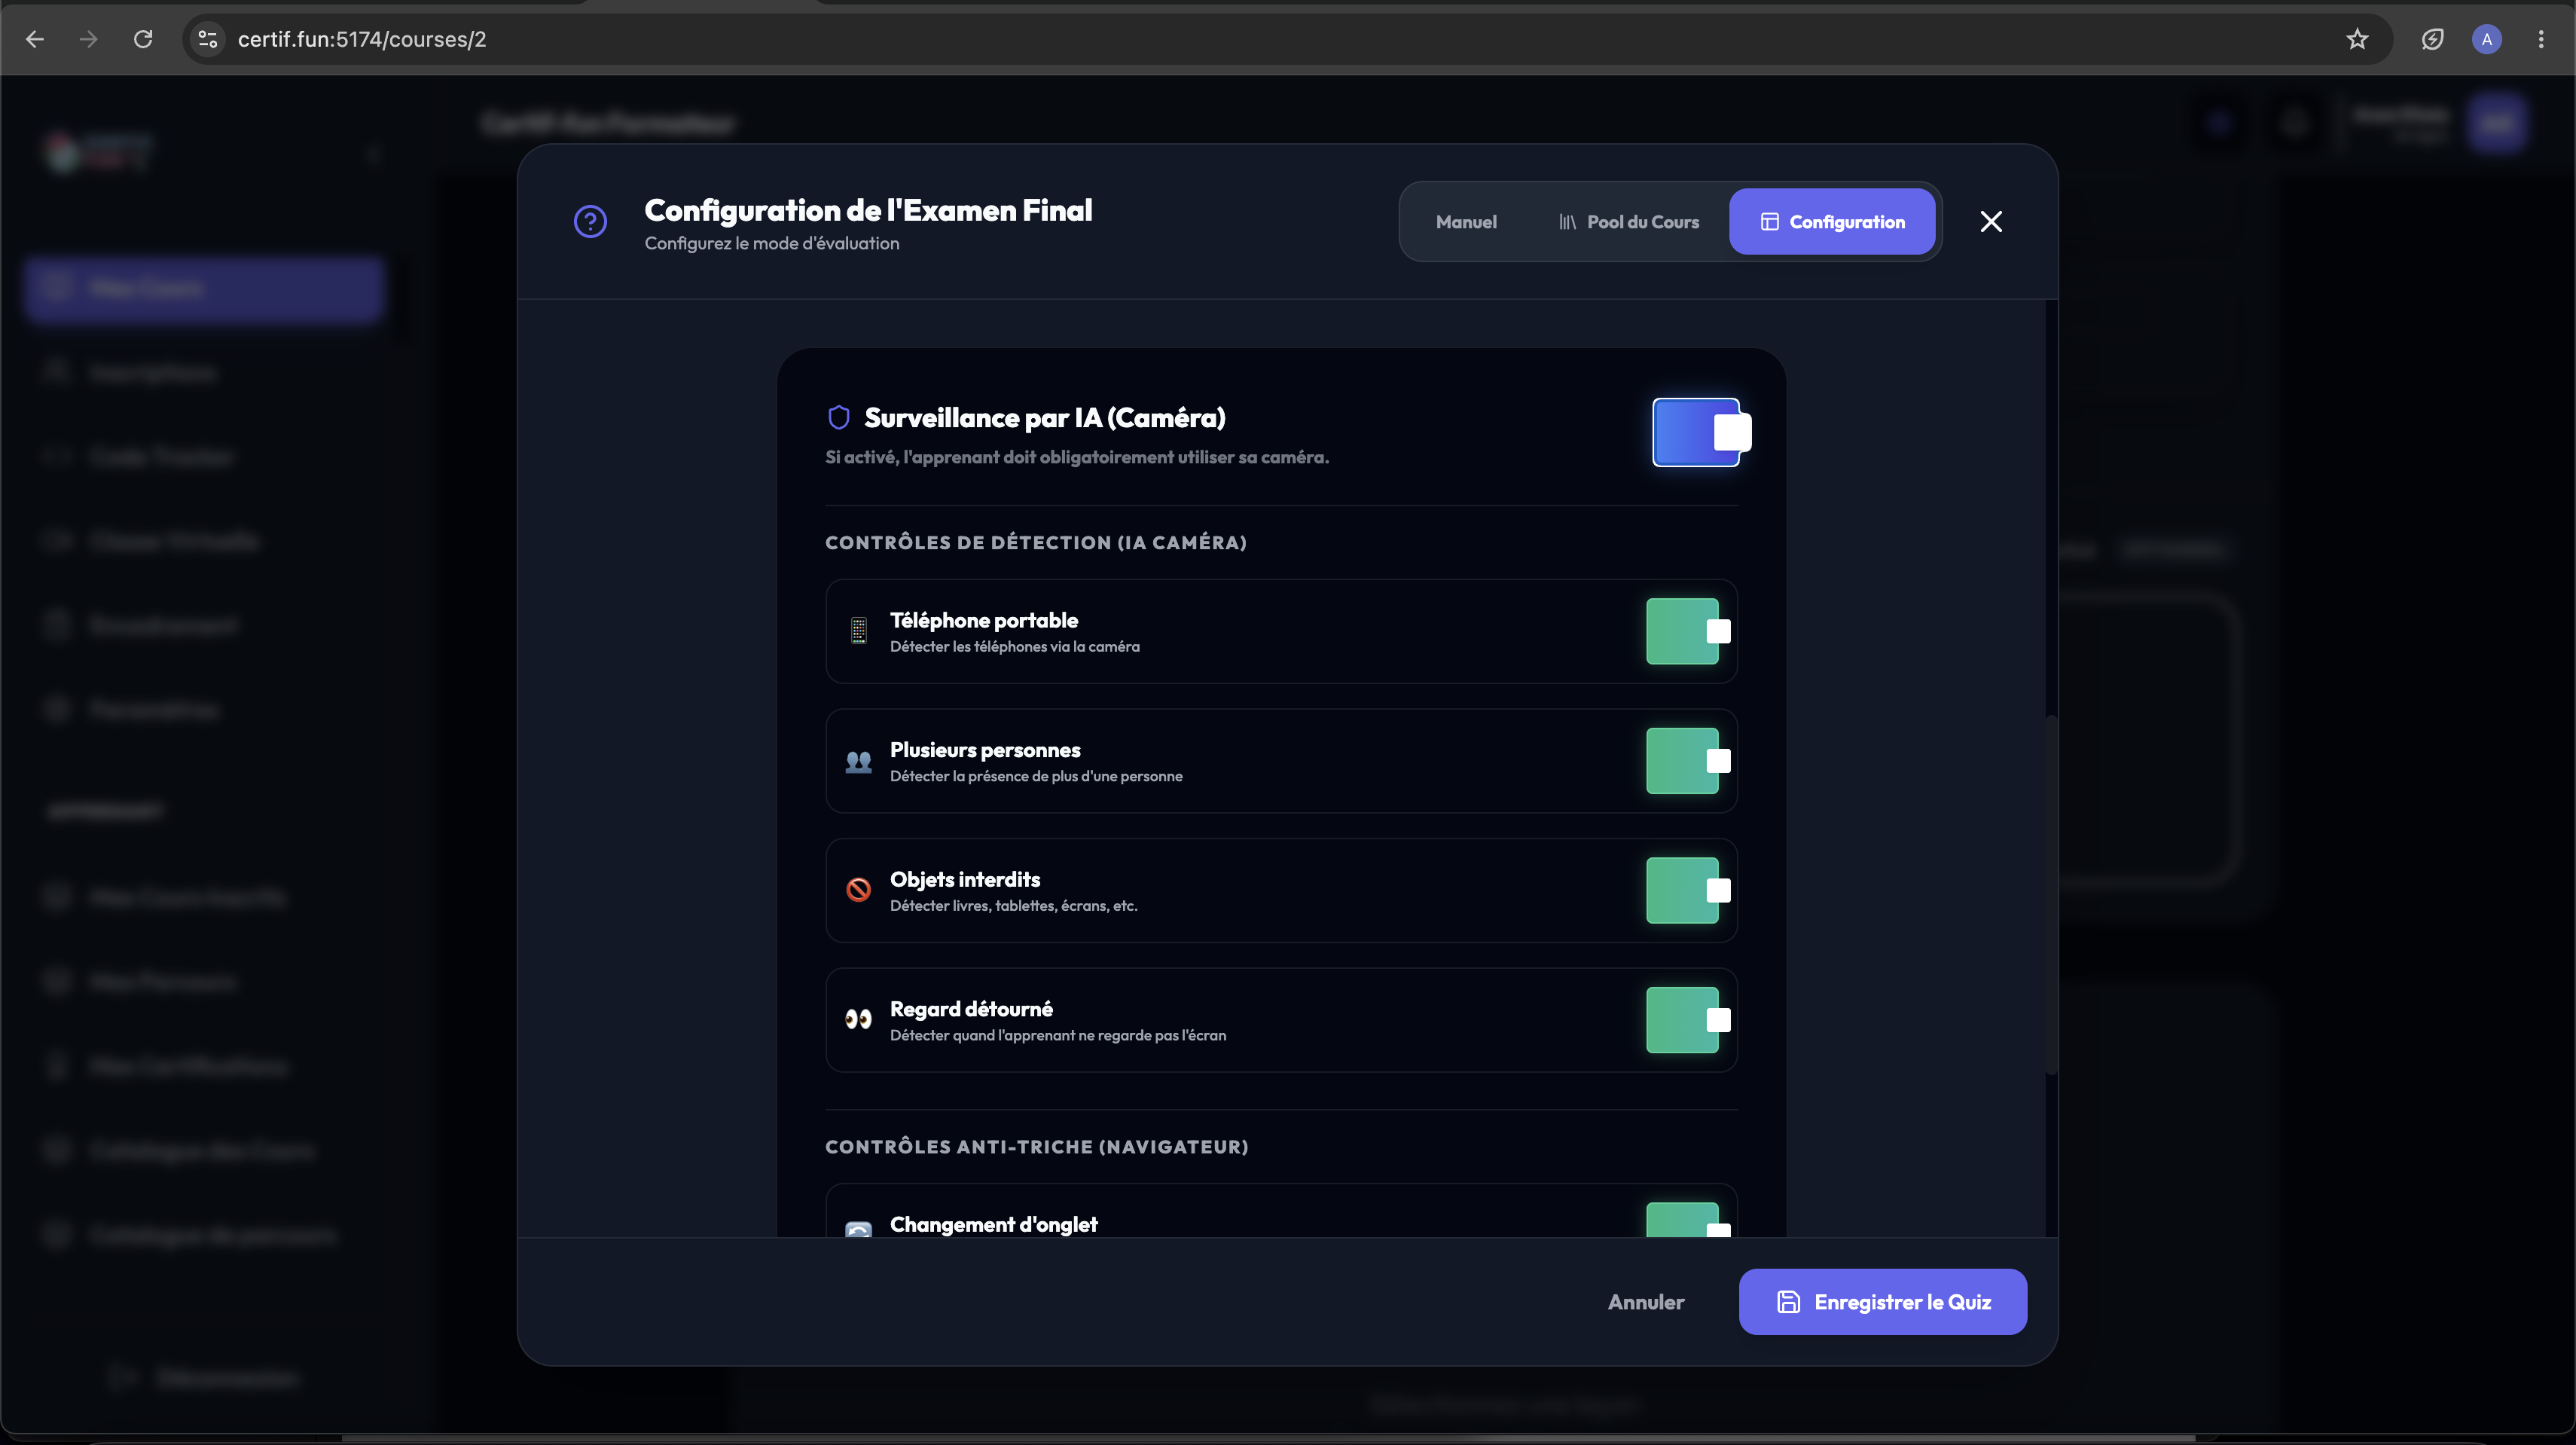
\includegraphics[width=0.98\textwidth]{figures/formateur-11.png}
    \caption{Configuration de la surveillance par IA et contrôles anti-triche}
    \label{fig:formateur11}
\end{figure}

\subsubsection{Portail Apprenant}
L'espace Apprenant vise à offrir une expérience d'apprentissage simple, organisée et efficace.

Le tableau de bord personnel (Figure~\ref{fig:apprenant1}) accueille l'étudiant avec un résumé de sa progression (cours inscrits, terminés, score moyen). Il lui propose un accès rapide pour continuer l'apprentissage et affiche l'historique de ses derniers résultats d'examens.
\begin{figure}[H]
    \centering
    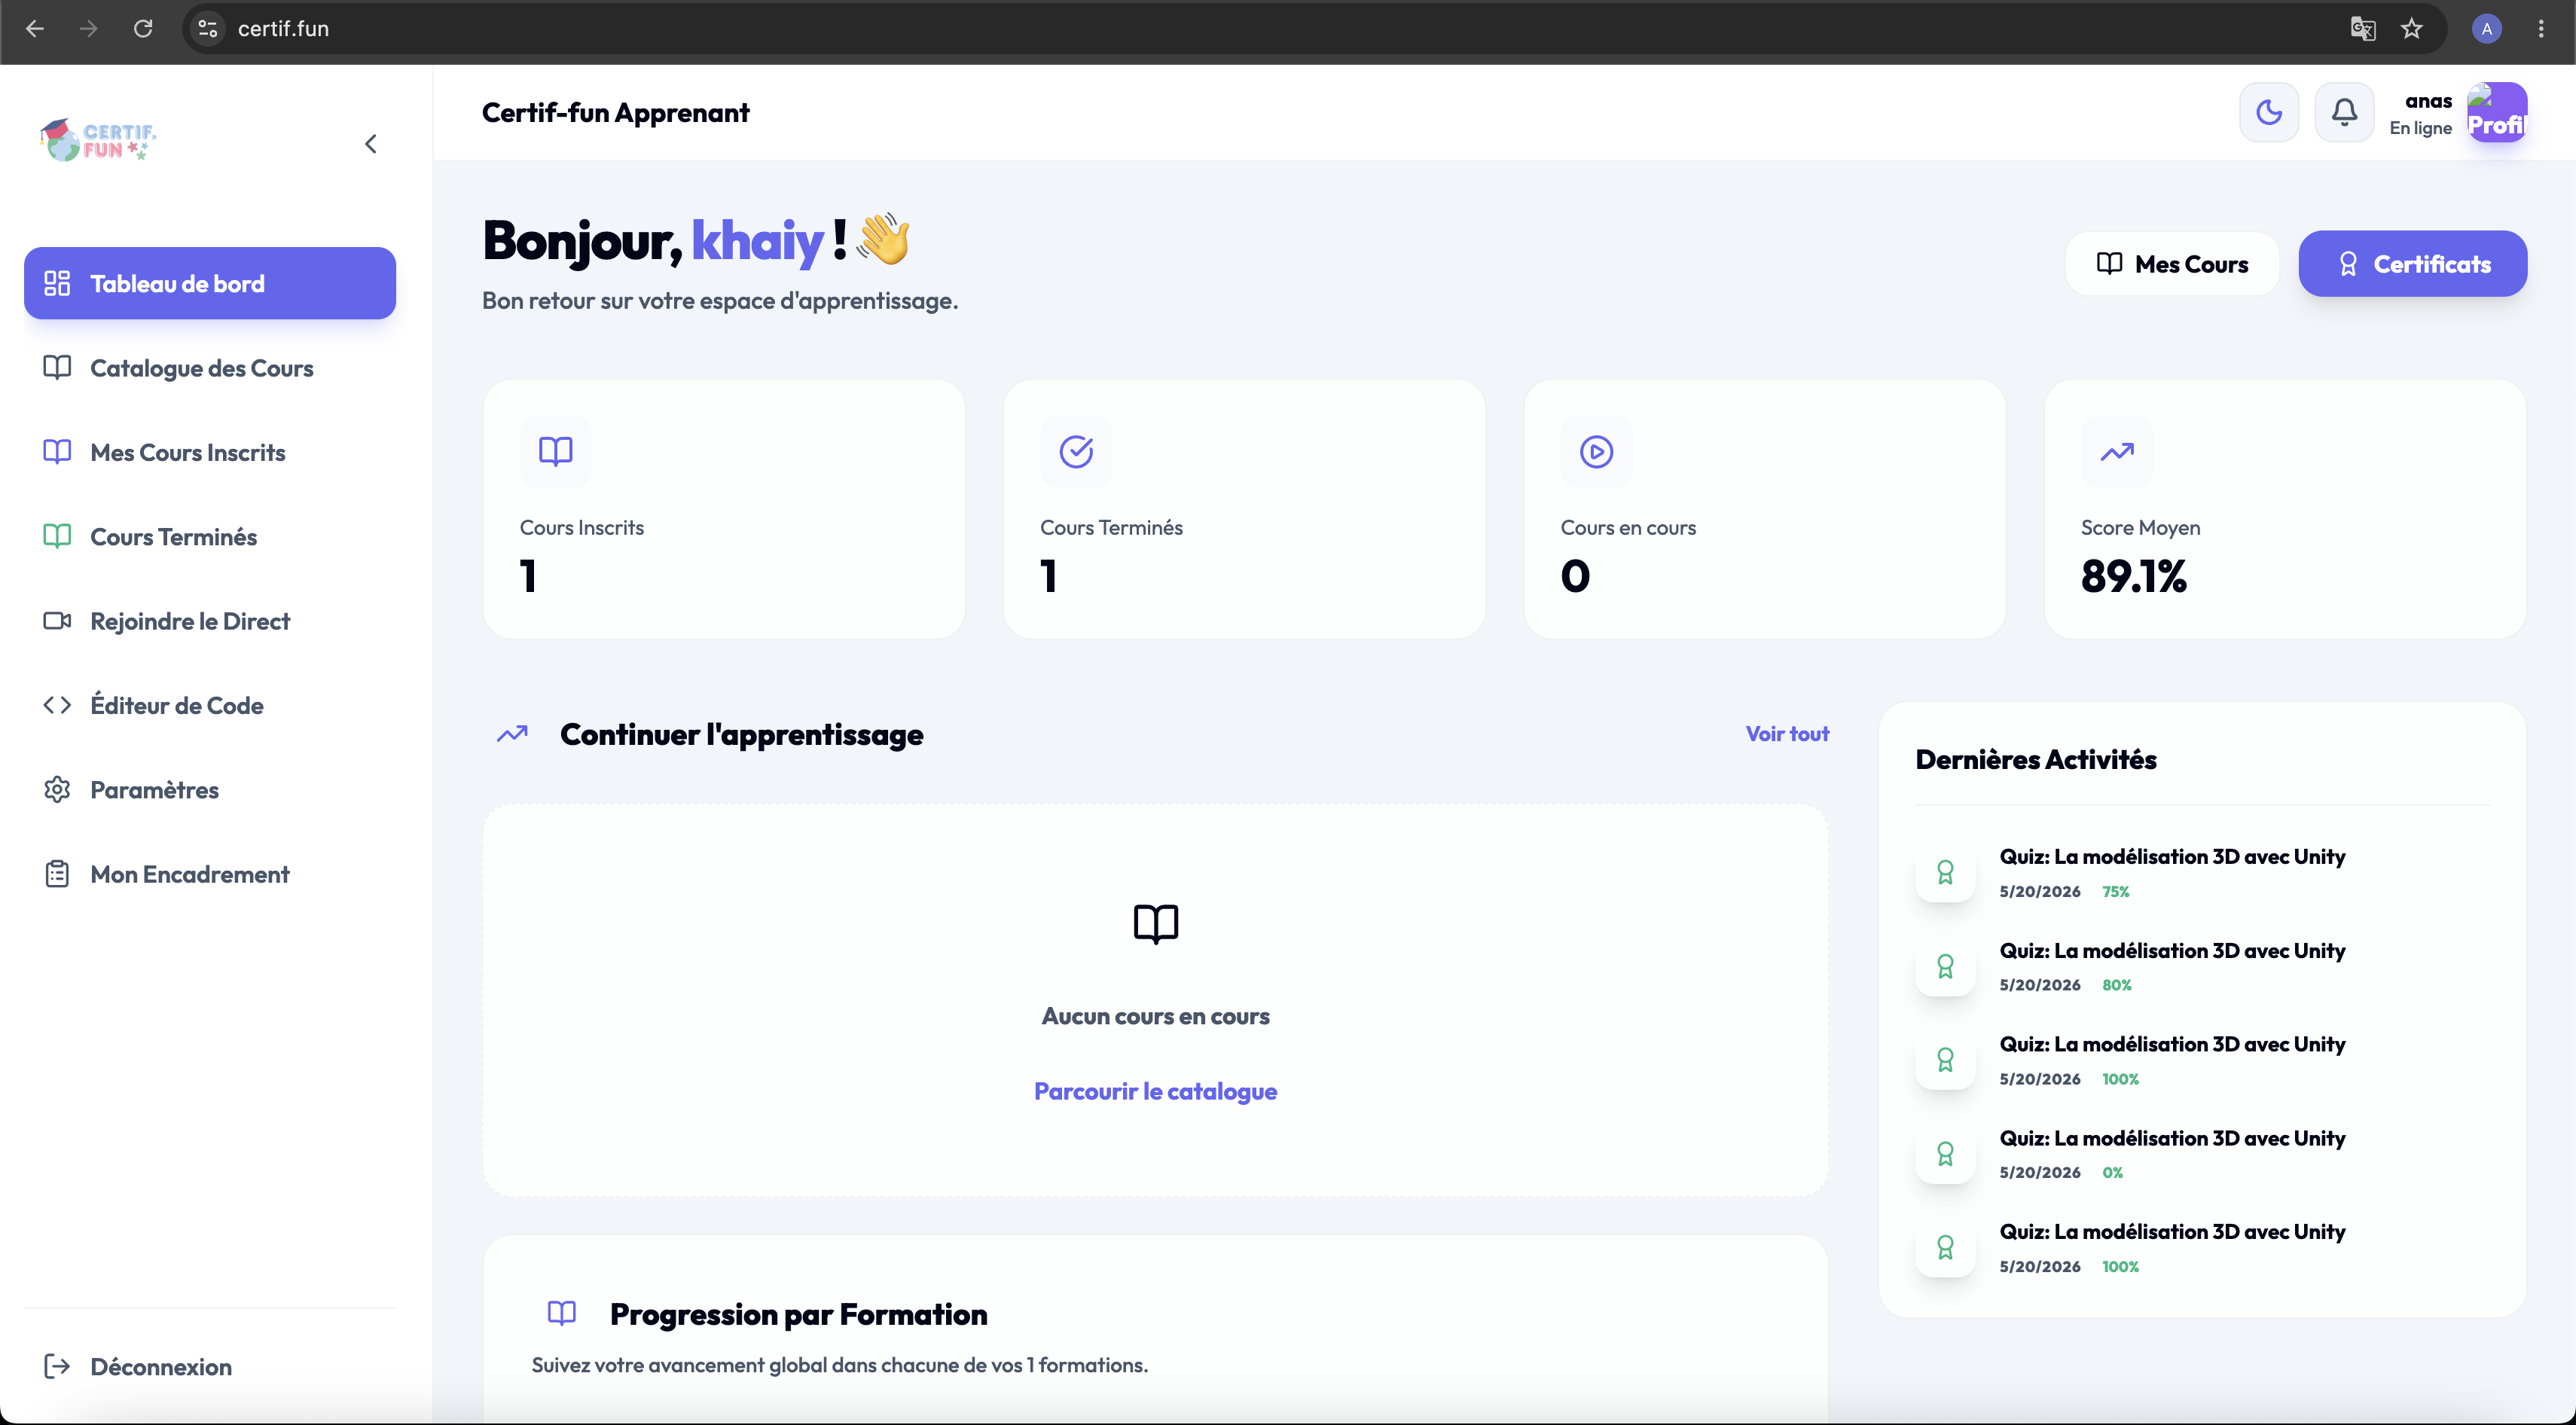
\includegraphics[width=0.98\textwidth]{figures/apprenant-1.png}
    \caption{Tableau de bord de l'Apprenant}
    \label{fig:apprenant1}
\end{figure}

Le catalogue de cours (Figure~\ref{fig:apprenant2}) permet à l'apprenant d'explorer toute l'offre de formation de la plateforme. Grâce à des filtres par catégorie ou niveau, il peut facilement trouver une nouvelle compétence à acquérir et s'y inscrire.
\begin{figure}[H]
    \centering
    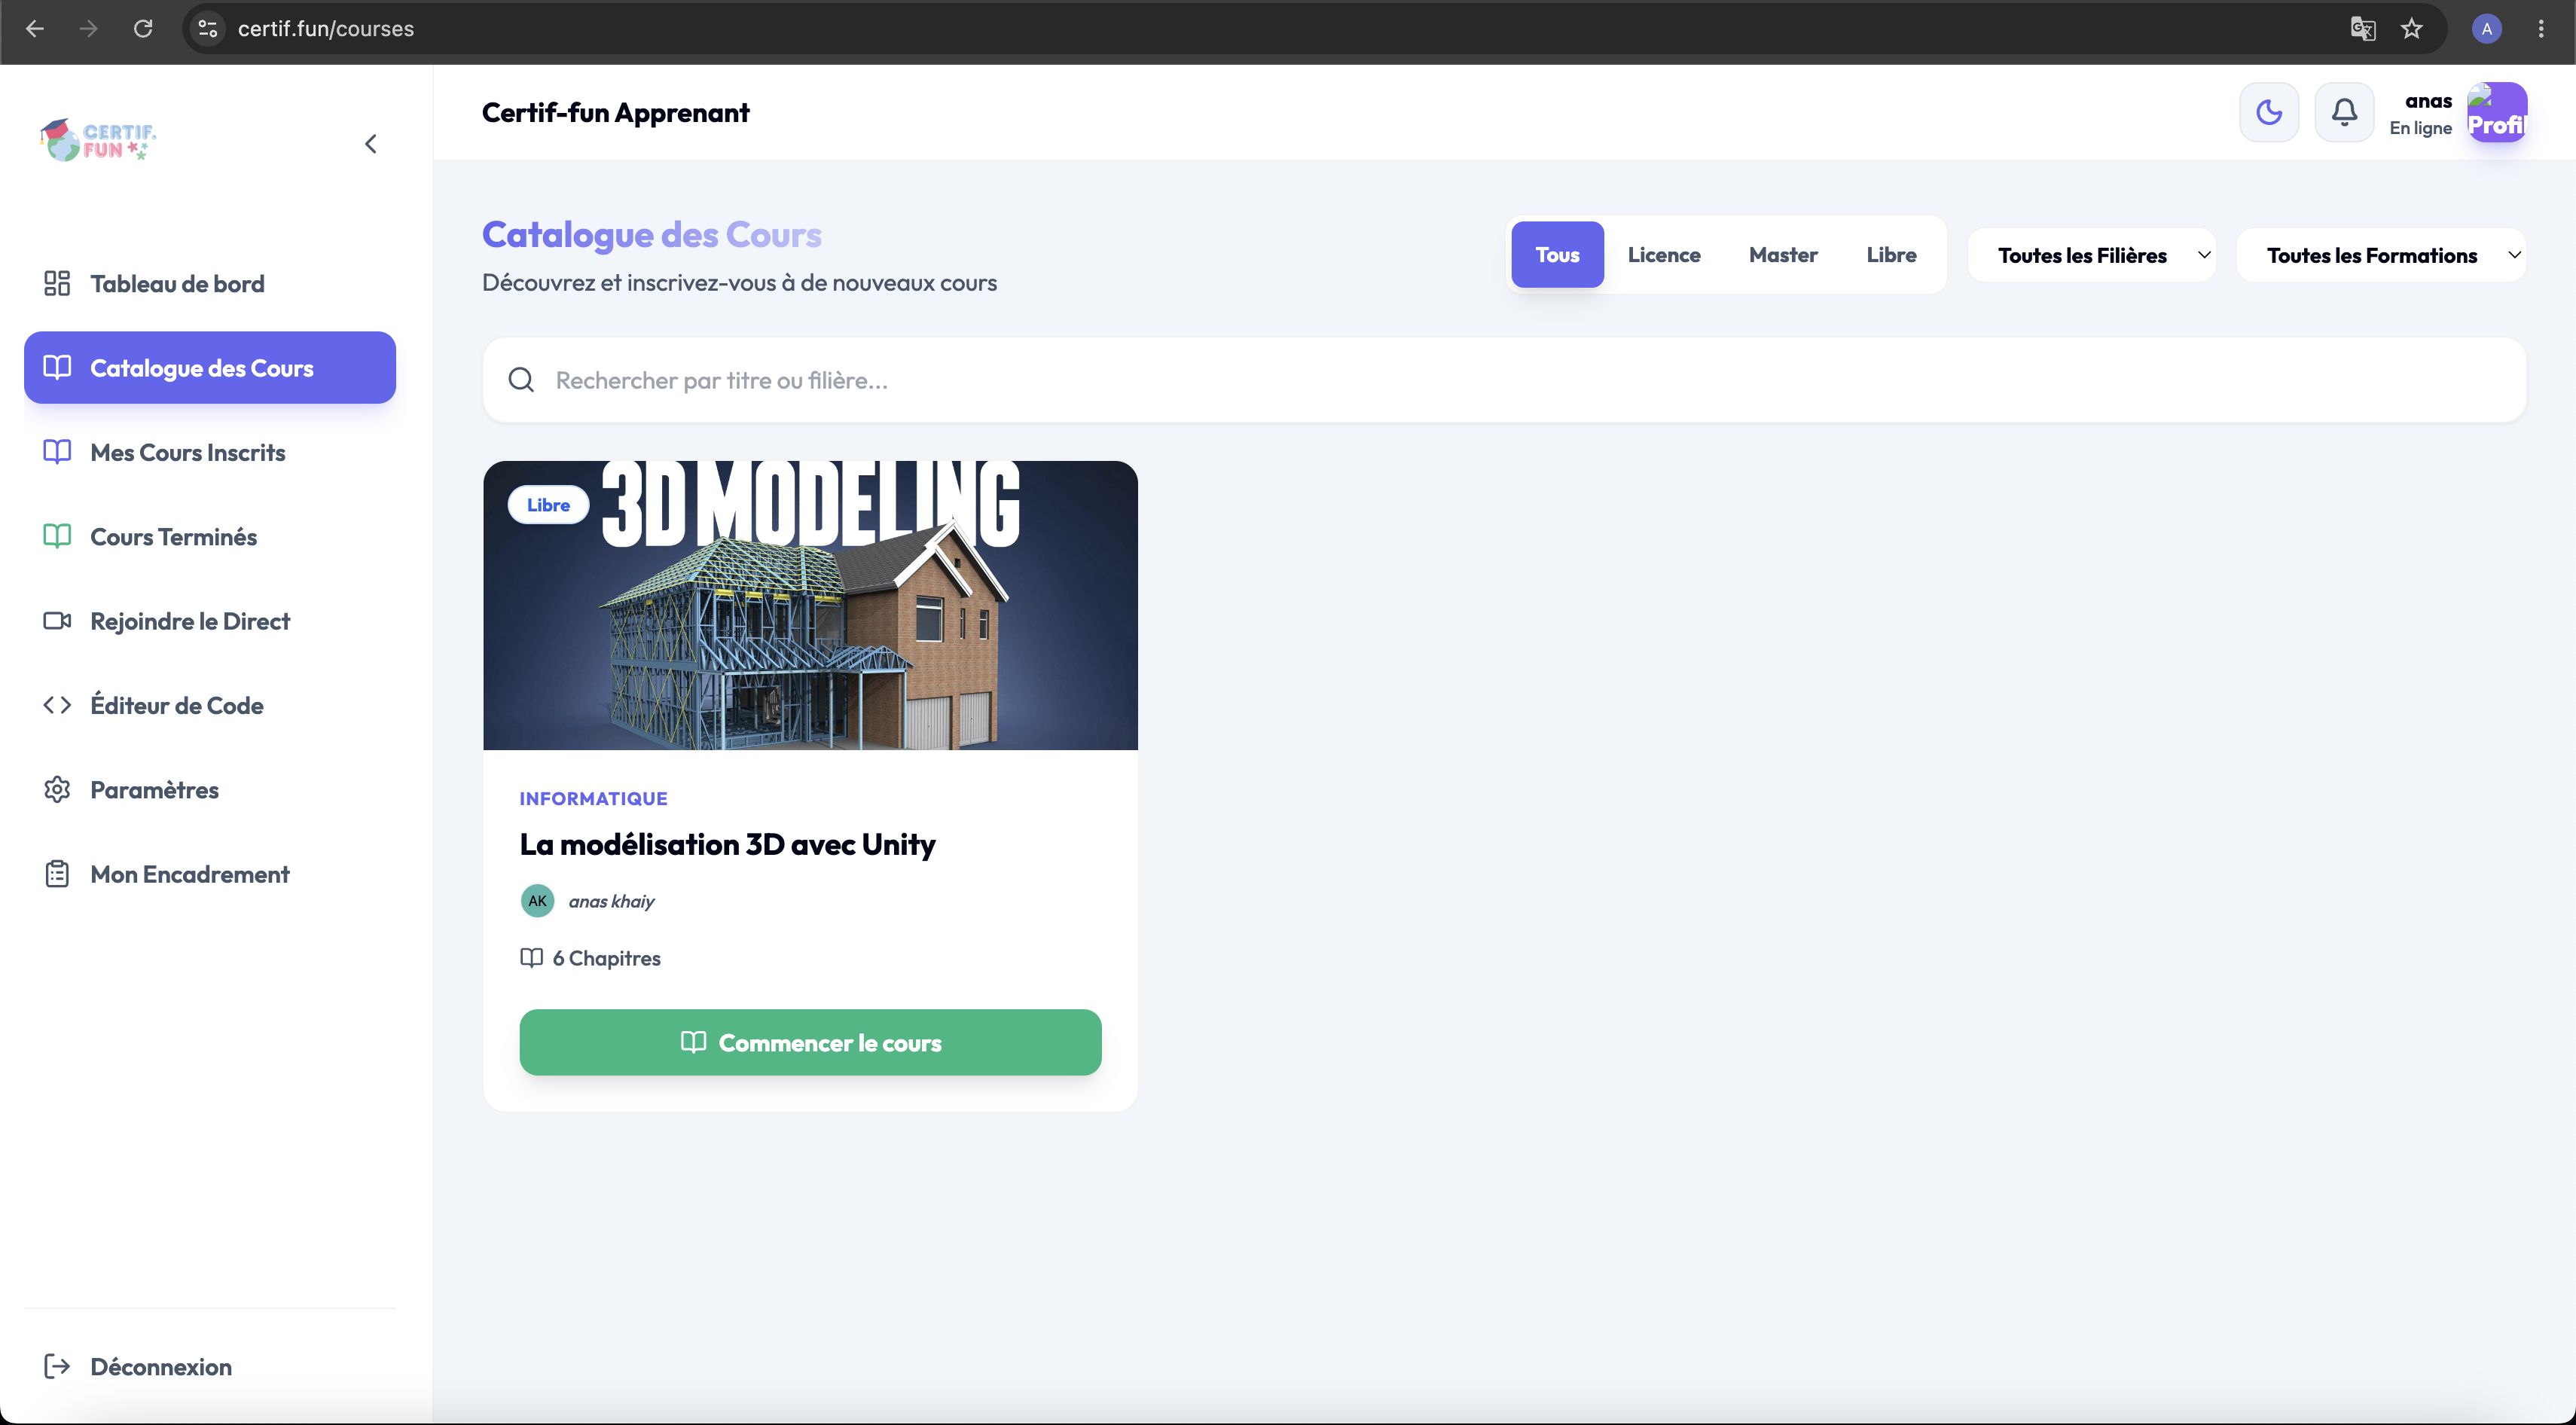
\includegraphics[width=0.98\textwidth]{figures/apprenant-2.png}
    \caption{Catalogue interactif des cours}
    \label{fig:apprenant2}
\end{figure}

Dans la rubrique "Cours Terminés" (Figure~\ref{fig:apprenant3}), l'apprenant retrouve l'ensemble des certificats qu'il a obtenus. Cette vue lui permet de visualiser son diplôme, de l'imprimer ou de le télécharger en version PDF.
\begin{figure}[H]
    \centering
    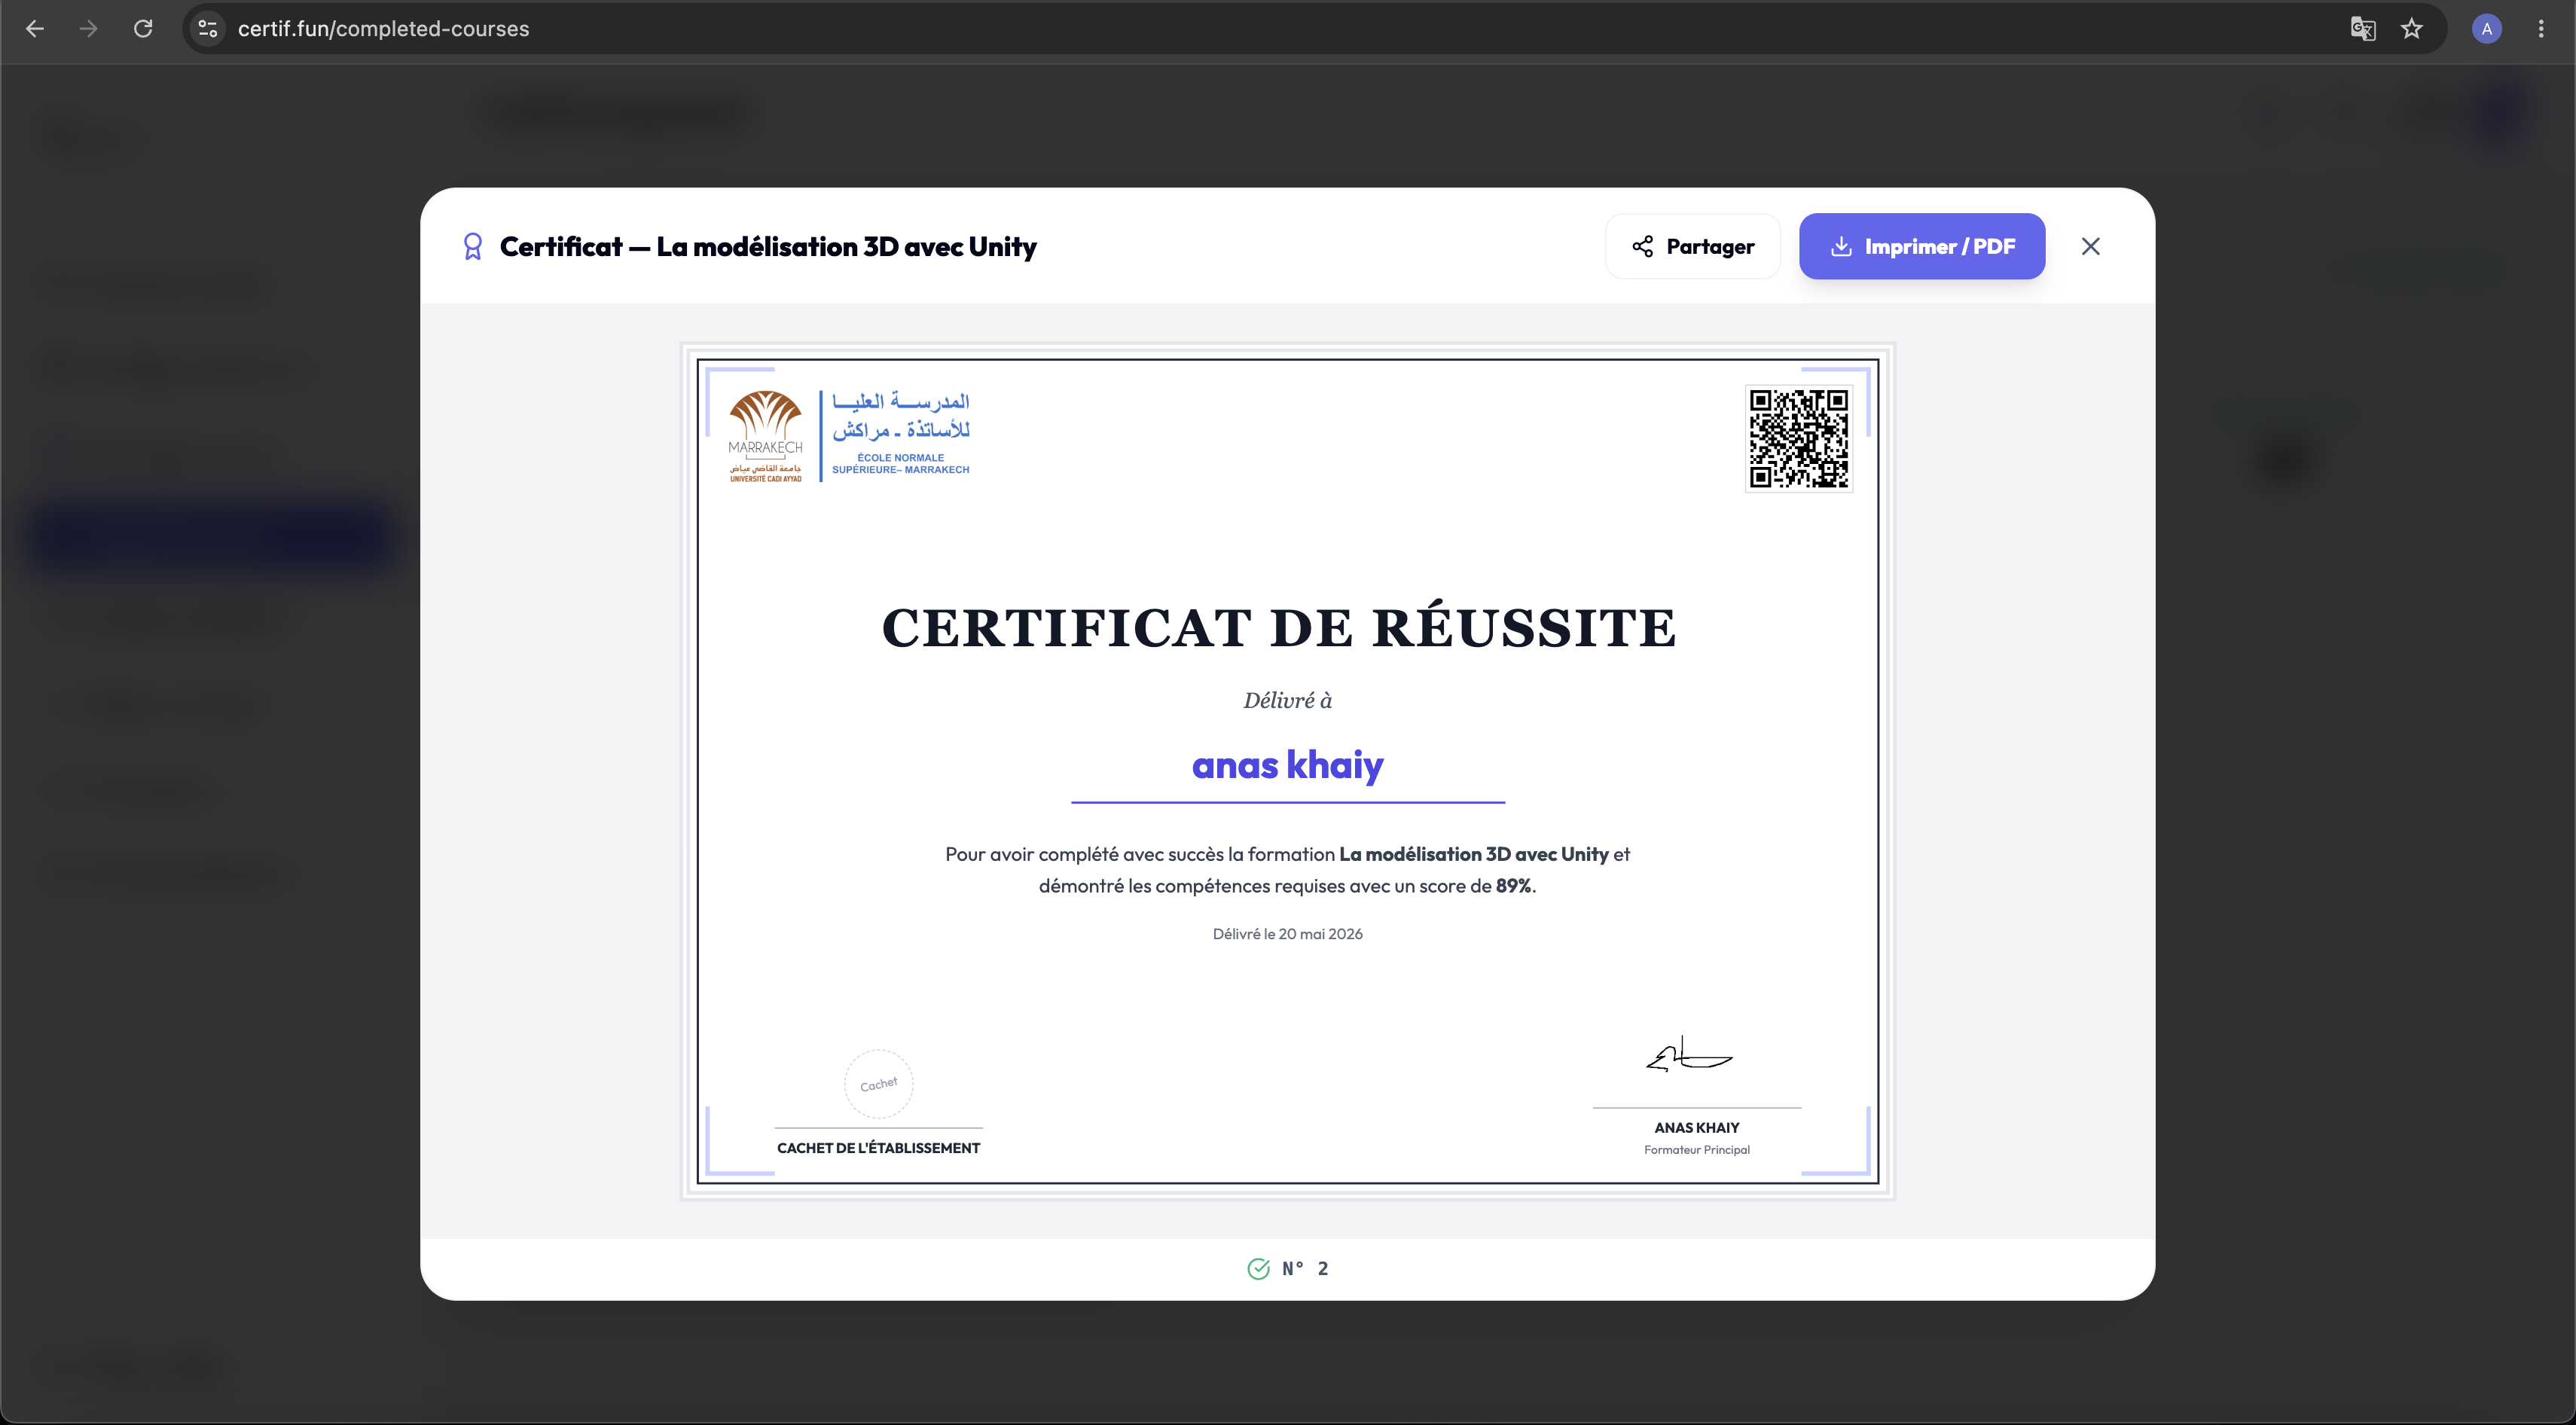
\includegraphics[width=0.98\textwidth]{figures/apprenant-3.png}
    \caption{Affichage et impression d'un certificat de réussite}
    \label{fig:apprenant3}
\end{figure}

L'onglet "Rejoindre le Direct" (Figure~\ref{fig:apprenant4}) permet à l'étudiant de se connecter à une classe virtuelle. En renseignant le code fourni par l'enseignant, il entre directement dans la salle de visioconférence pour suivre son cours en temps réel.
\begin{figure}[H]
    \centering
    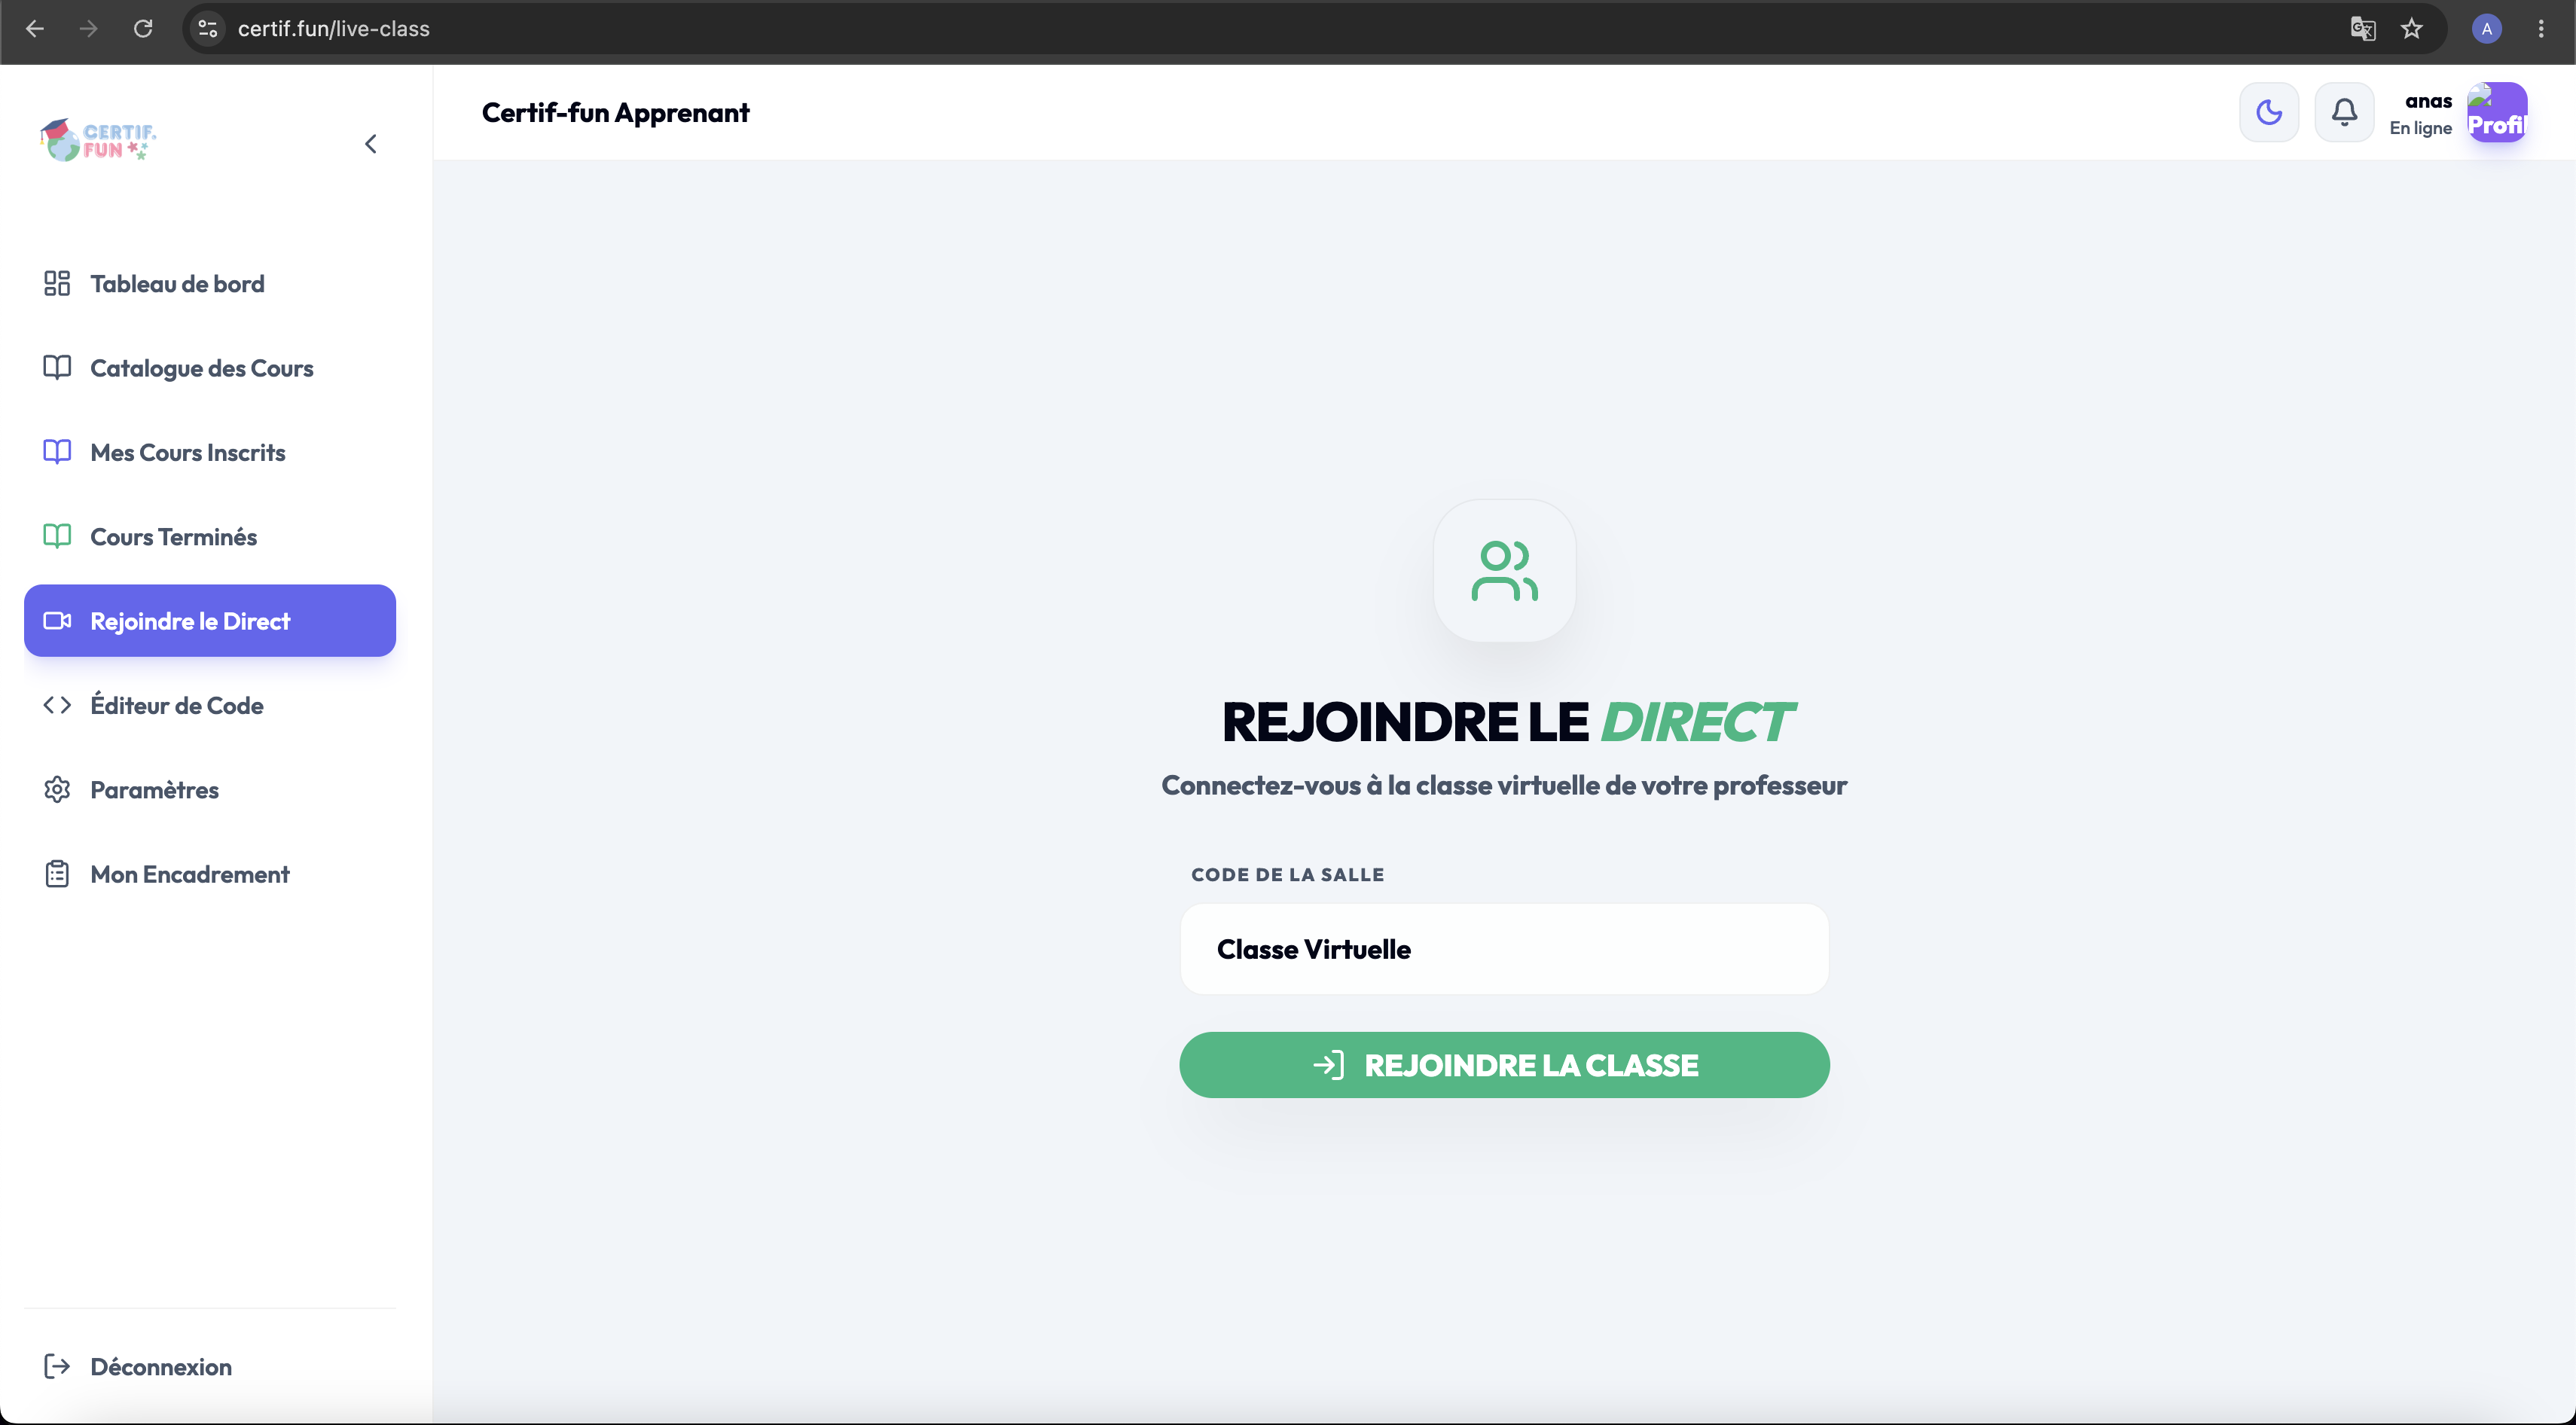
\includegraphics[width=0.98\textwidth]{figures/apprenant-4.png}
    \caption{Connexion à une session d'enseignement en direct}
    \label{fig:apprenant4}
\end{figure}

Pour les exercices pratiques en informatique, l'application propose un "Éditeur de Code" intégré (Figure~\ref{fig:apprenant5}). L'apprenant peut y rédiger et exécuter son code source de manière sécurisée (Sandbox) dans des langages comme Python, JavaScript ou Java.
\begin{figure}[H]
    \centering
    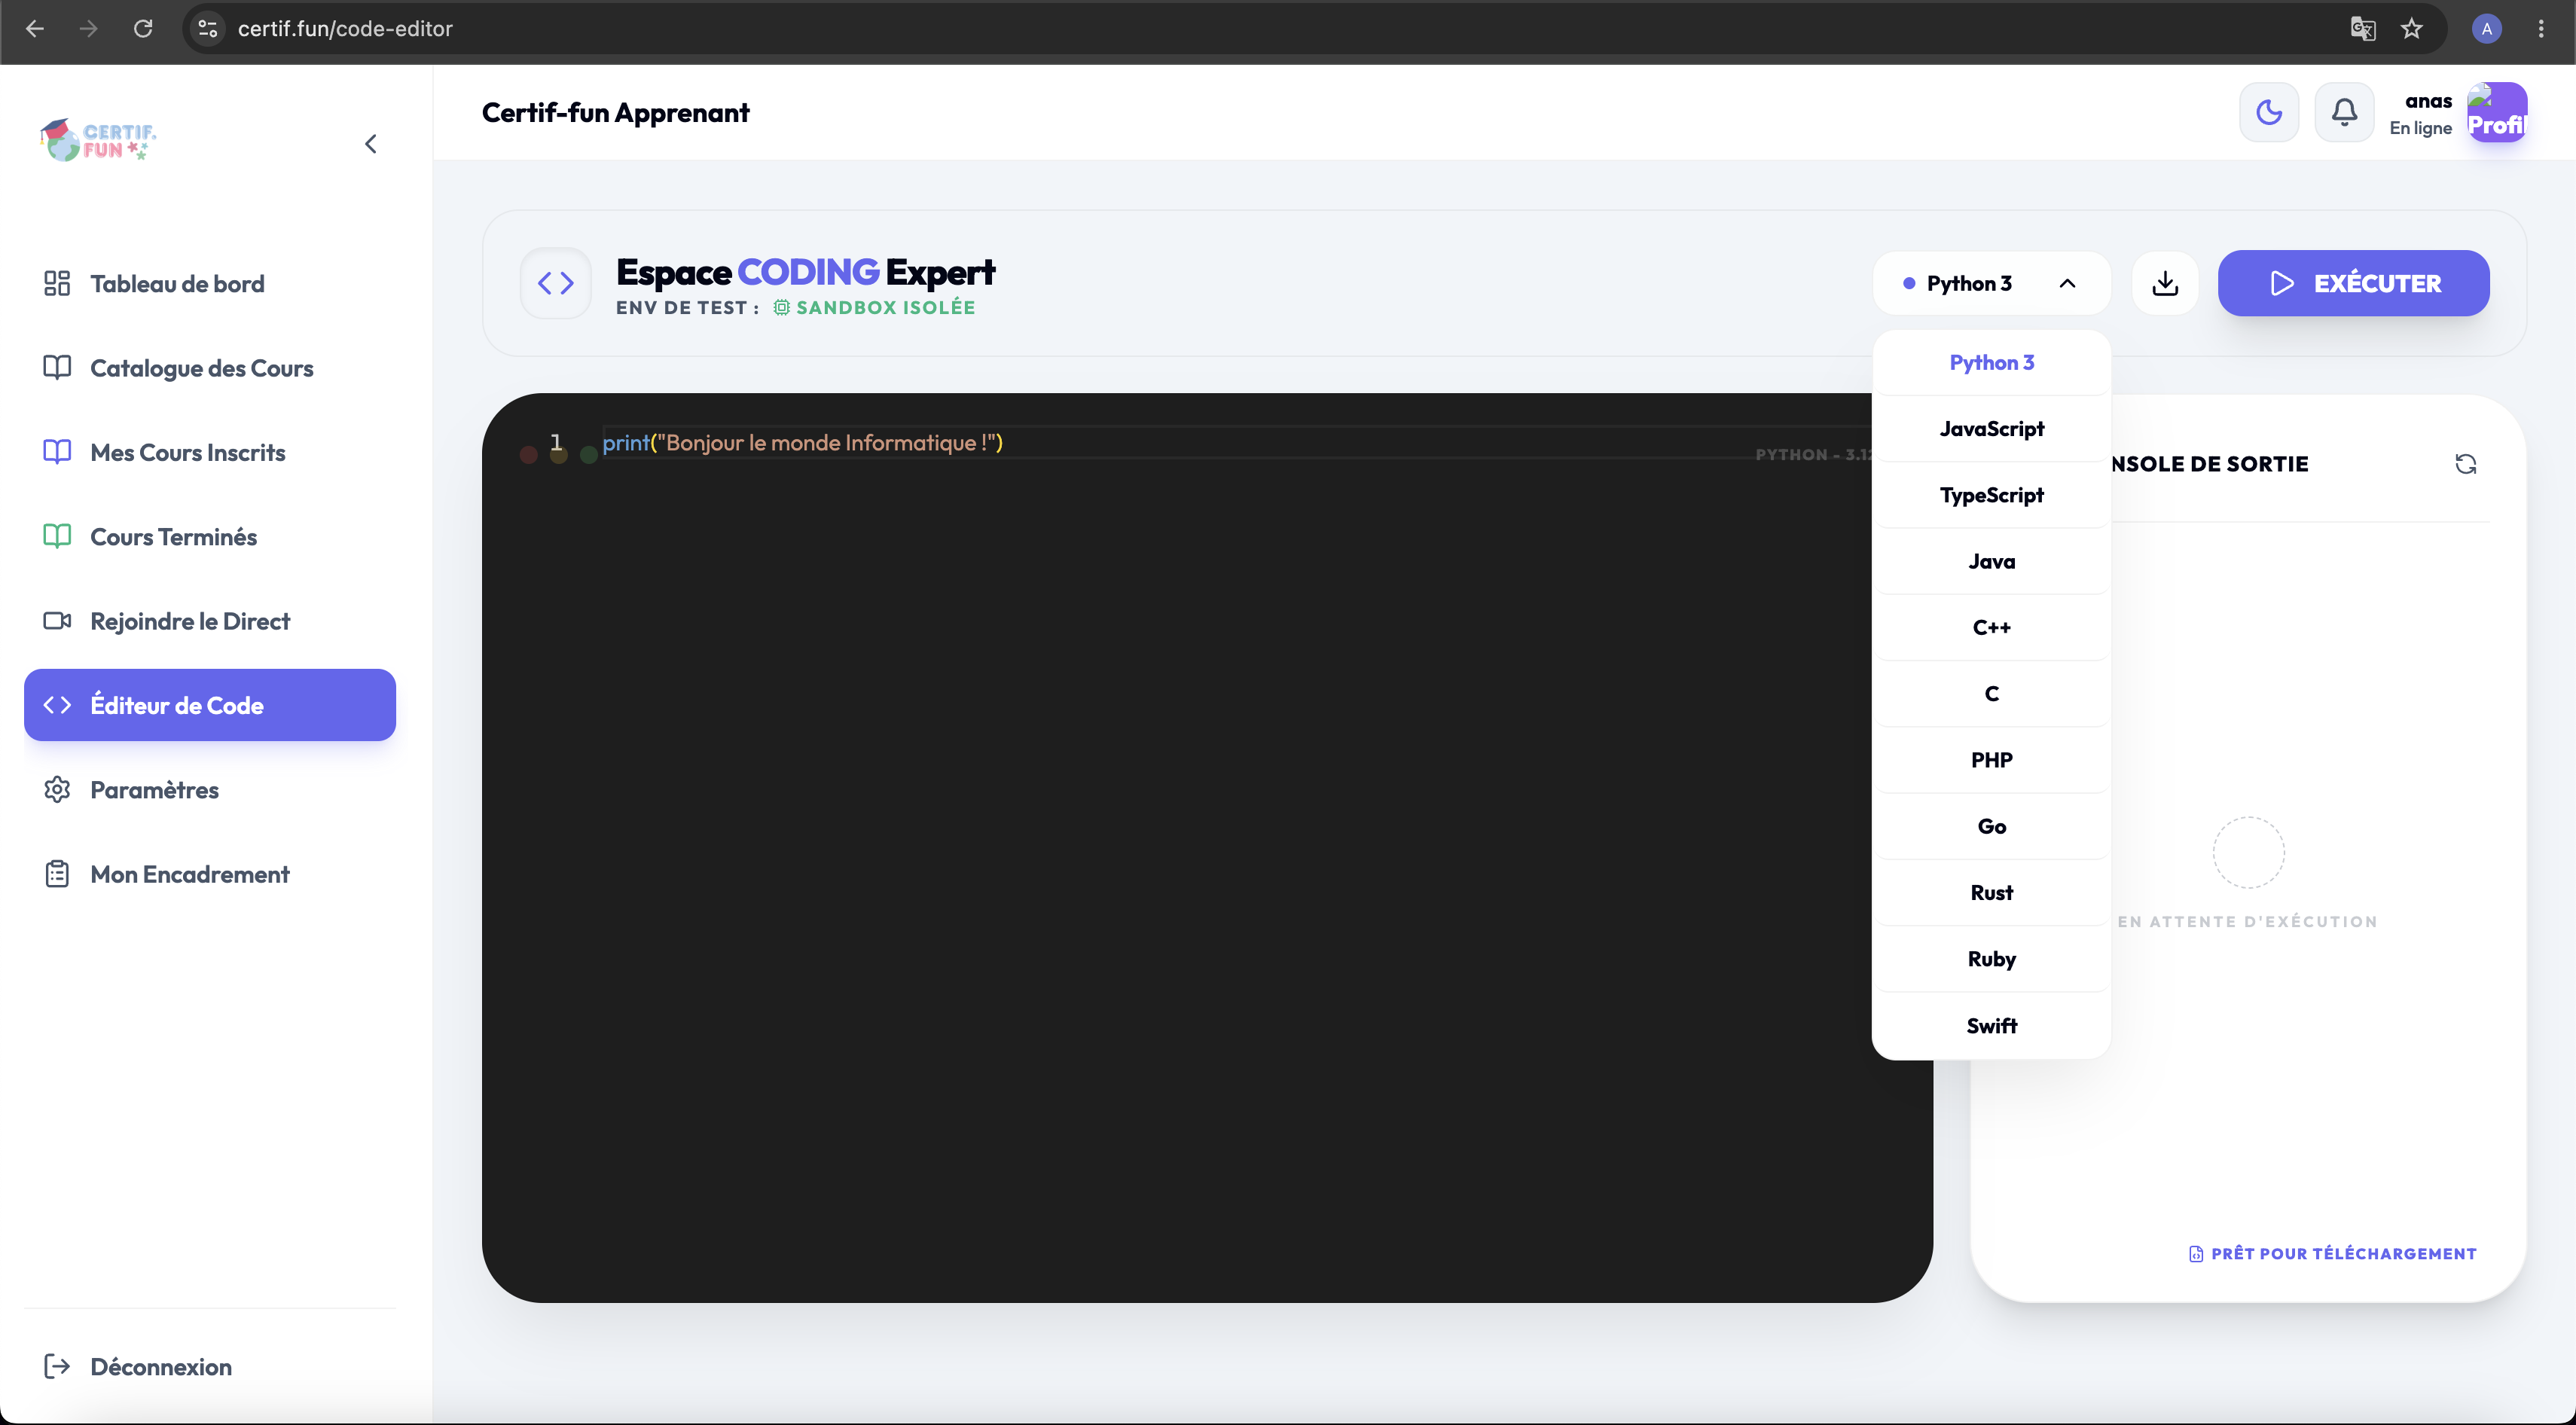
\includegraphics[width=0.98\textwidth]{figures/apprenant-5.png}
    \caption{Éditeur de code en ligne (Espace CODING Expert)}
    \label{fig:apprenant5}
\end{figure}

Enfin, le module "Mon Encadrement" (Figure~\ref{fig:apprenant6}) offre à l'étudiant un espace dédié pour la gestion de son projet de fin d'études. Il peut y visualiser sa barre de progression, ses tâches à faire et interagir avec son encadrant tout au long du projet.
\begin{figure}[H]
    \centering
    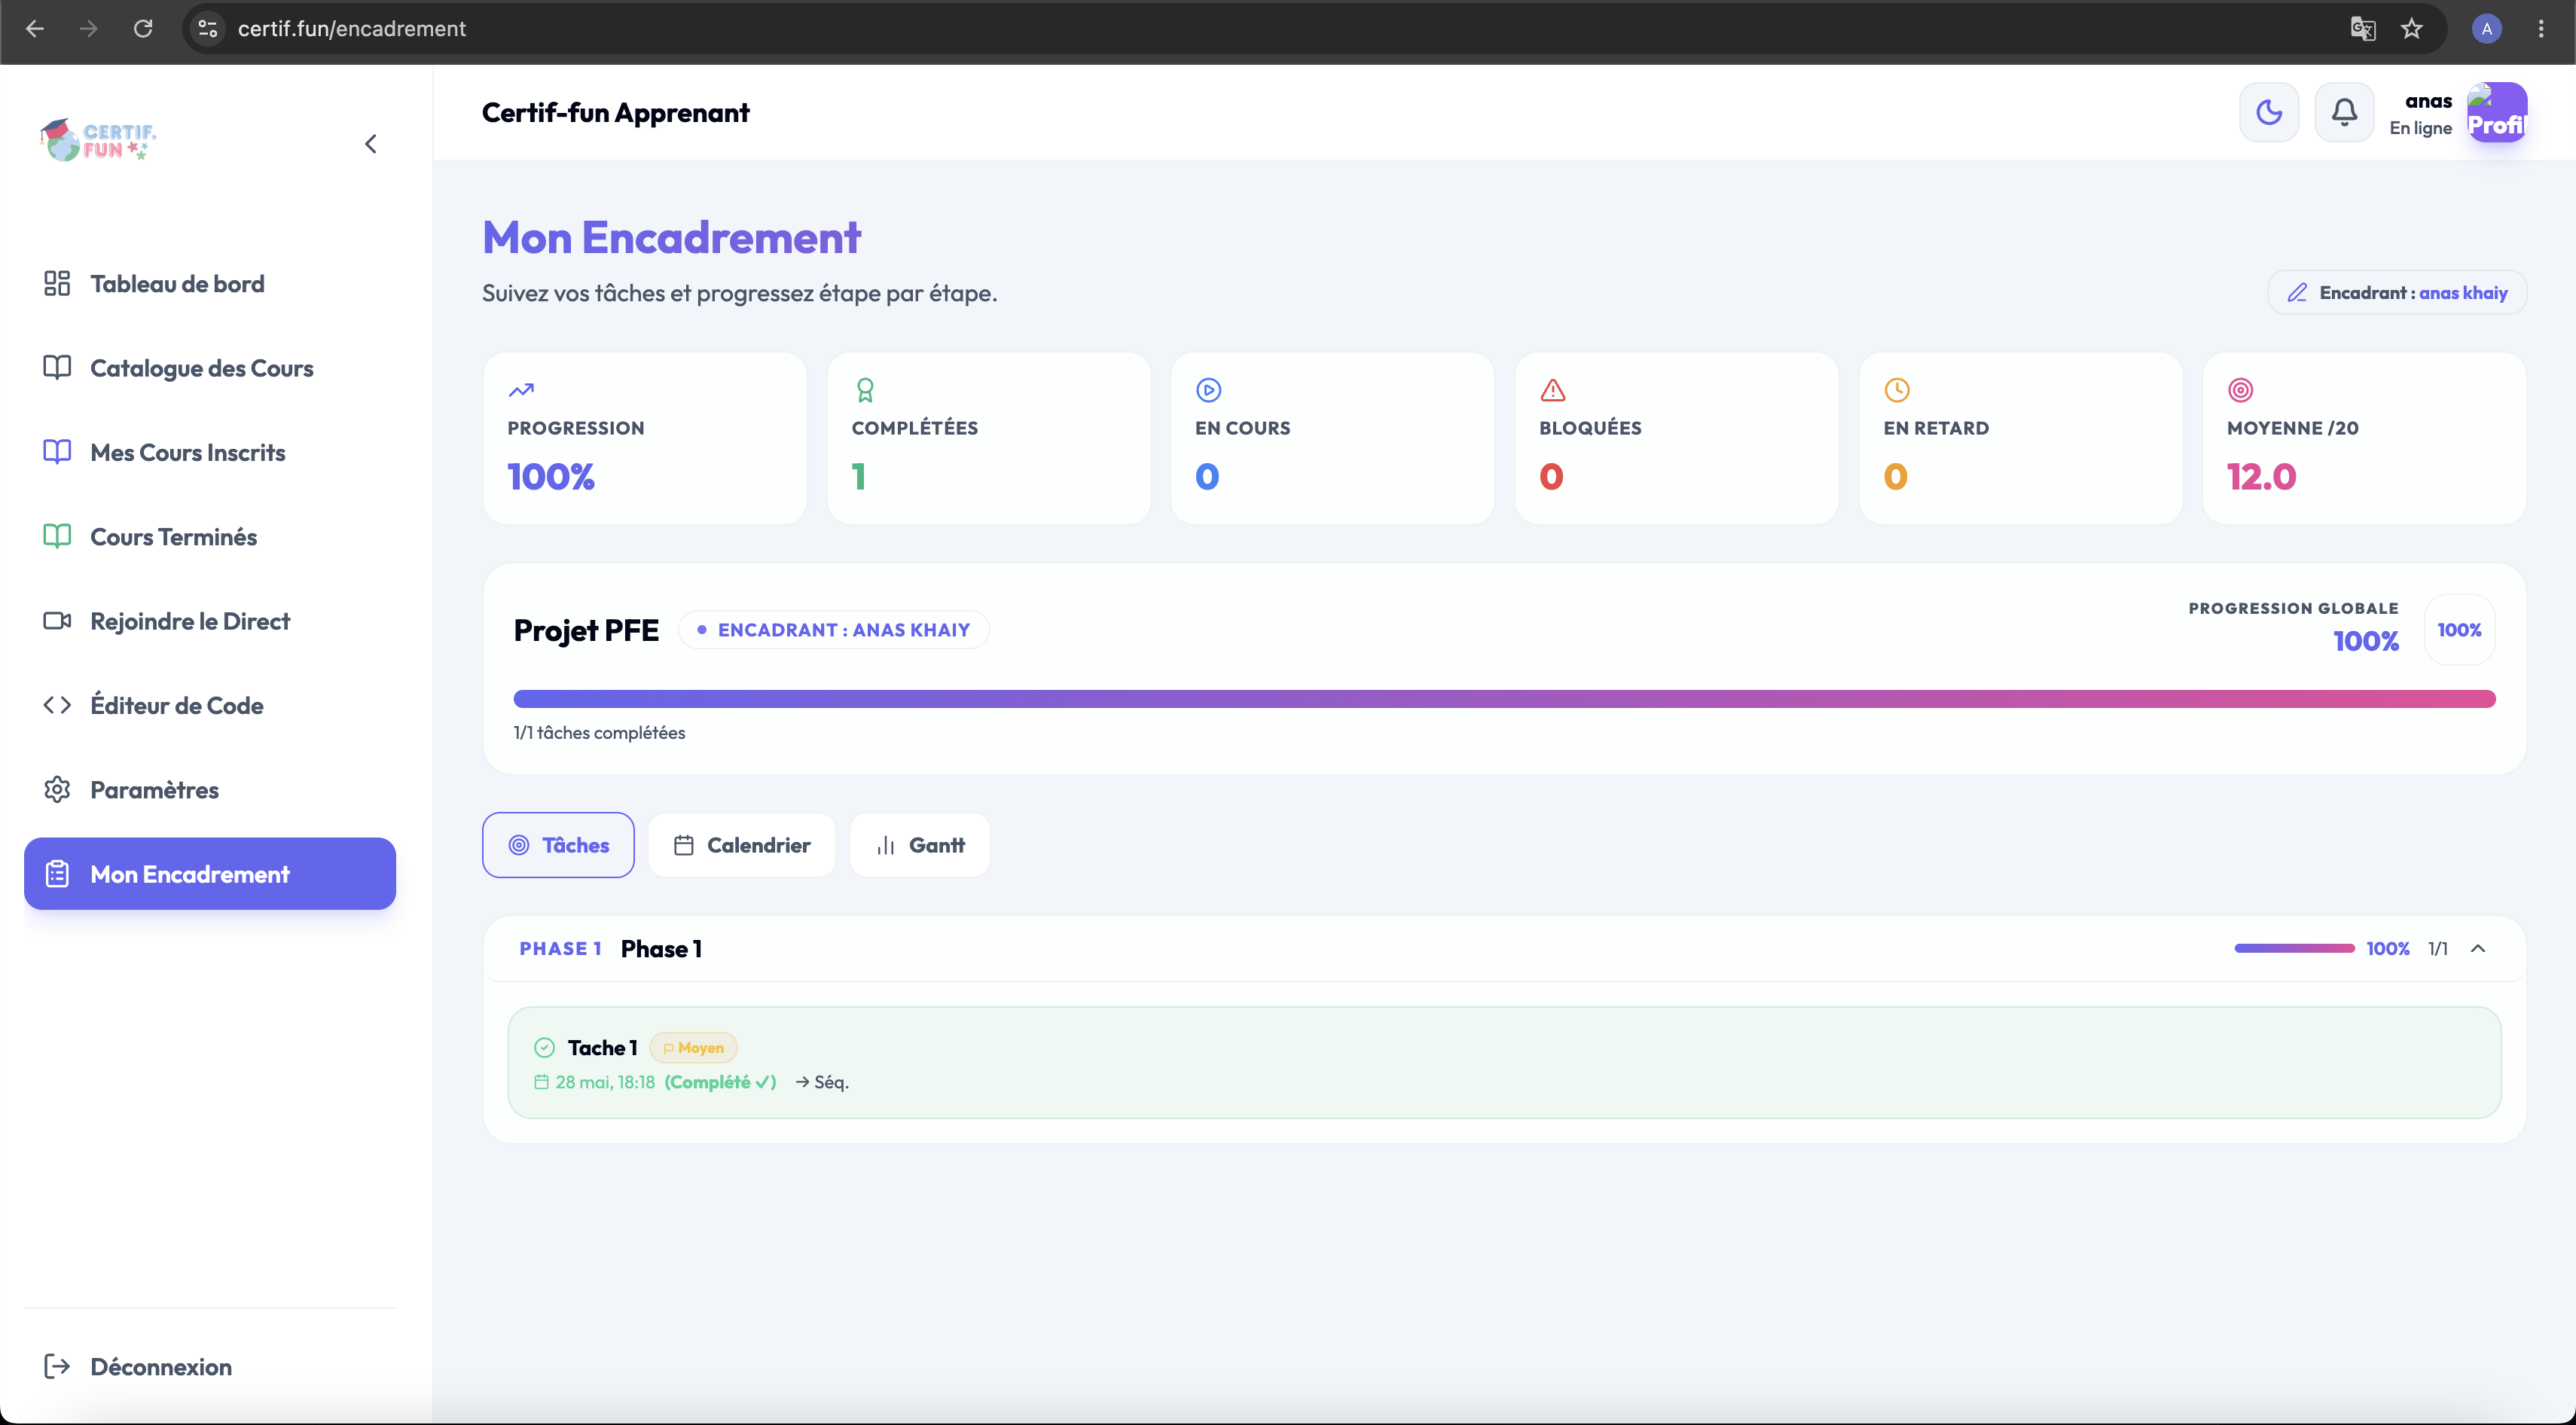
\includegraphics[width=0.98\textwidth]{figures/apprenant-6.png}
    \caption{Suivi personnalisé de l'encadrement des projets}
    \label{fig:apprenant6}
\end{figure}

L'espace d'apprentissage ou lecteur de cours (Figure~\ref{fig:apprenant7}) permet à l'étudiant de suivre le contenu pédagogique. Il dispose d'un menu de navigation latéral pour accéder aux différentes leçons et suivre sa progression. La zone principale affiche le contenu multimédia, comme des vidéos intégrées, accompagnées de textes explicatifs.
\begin{figure}[H]
    \centering
    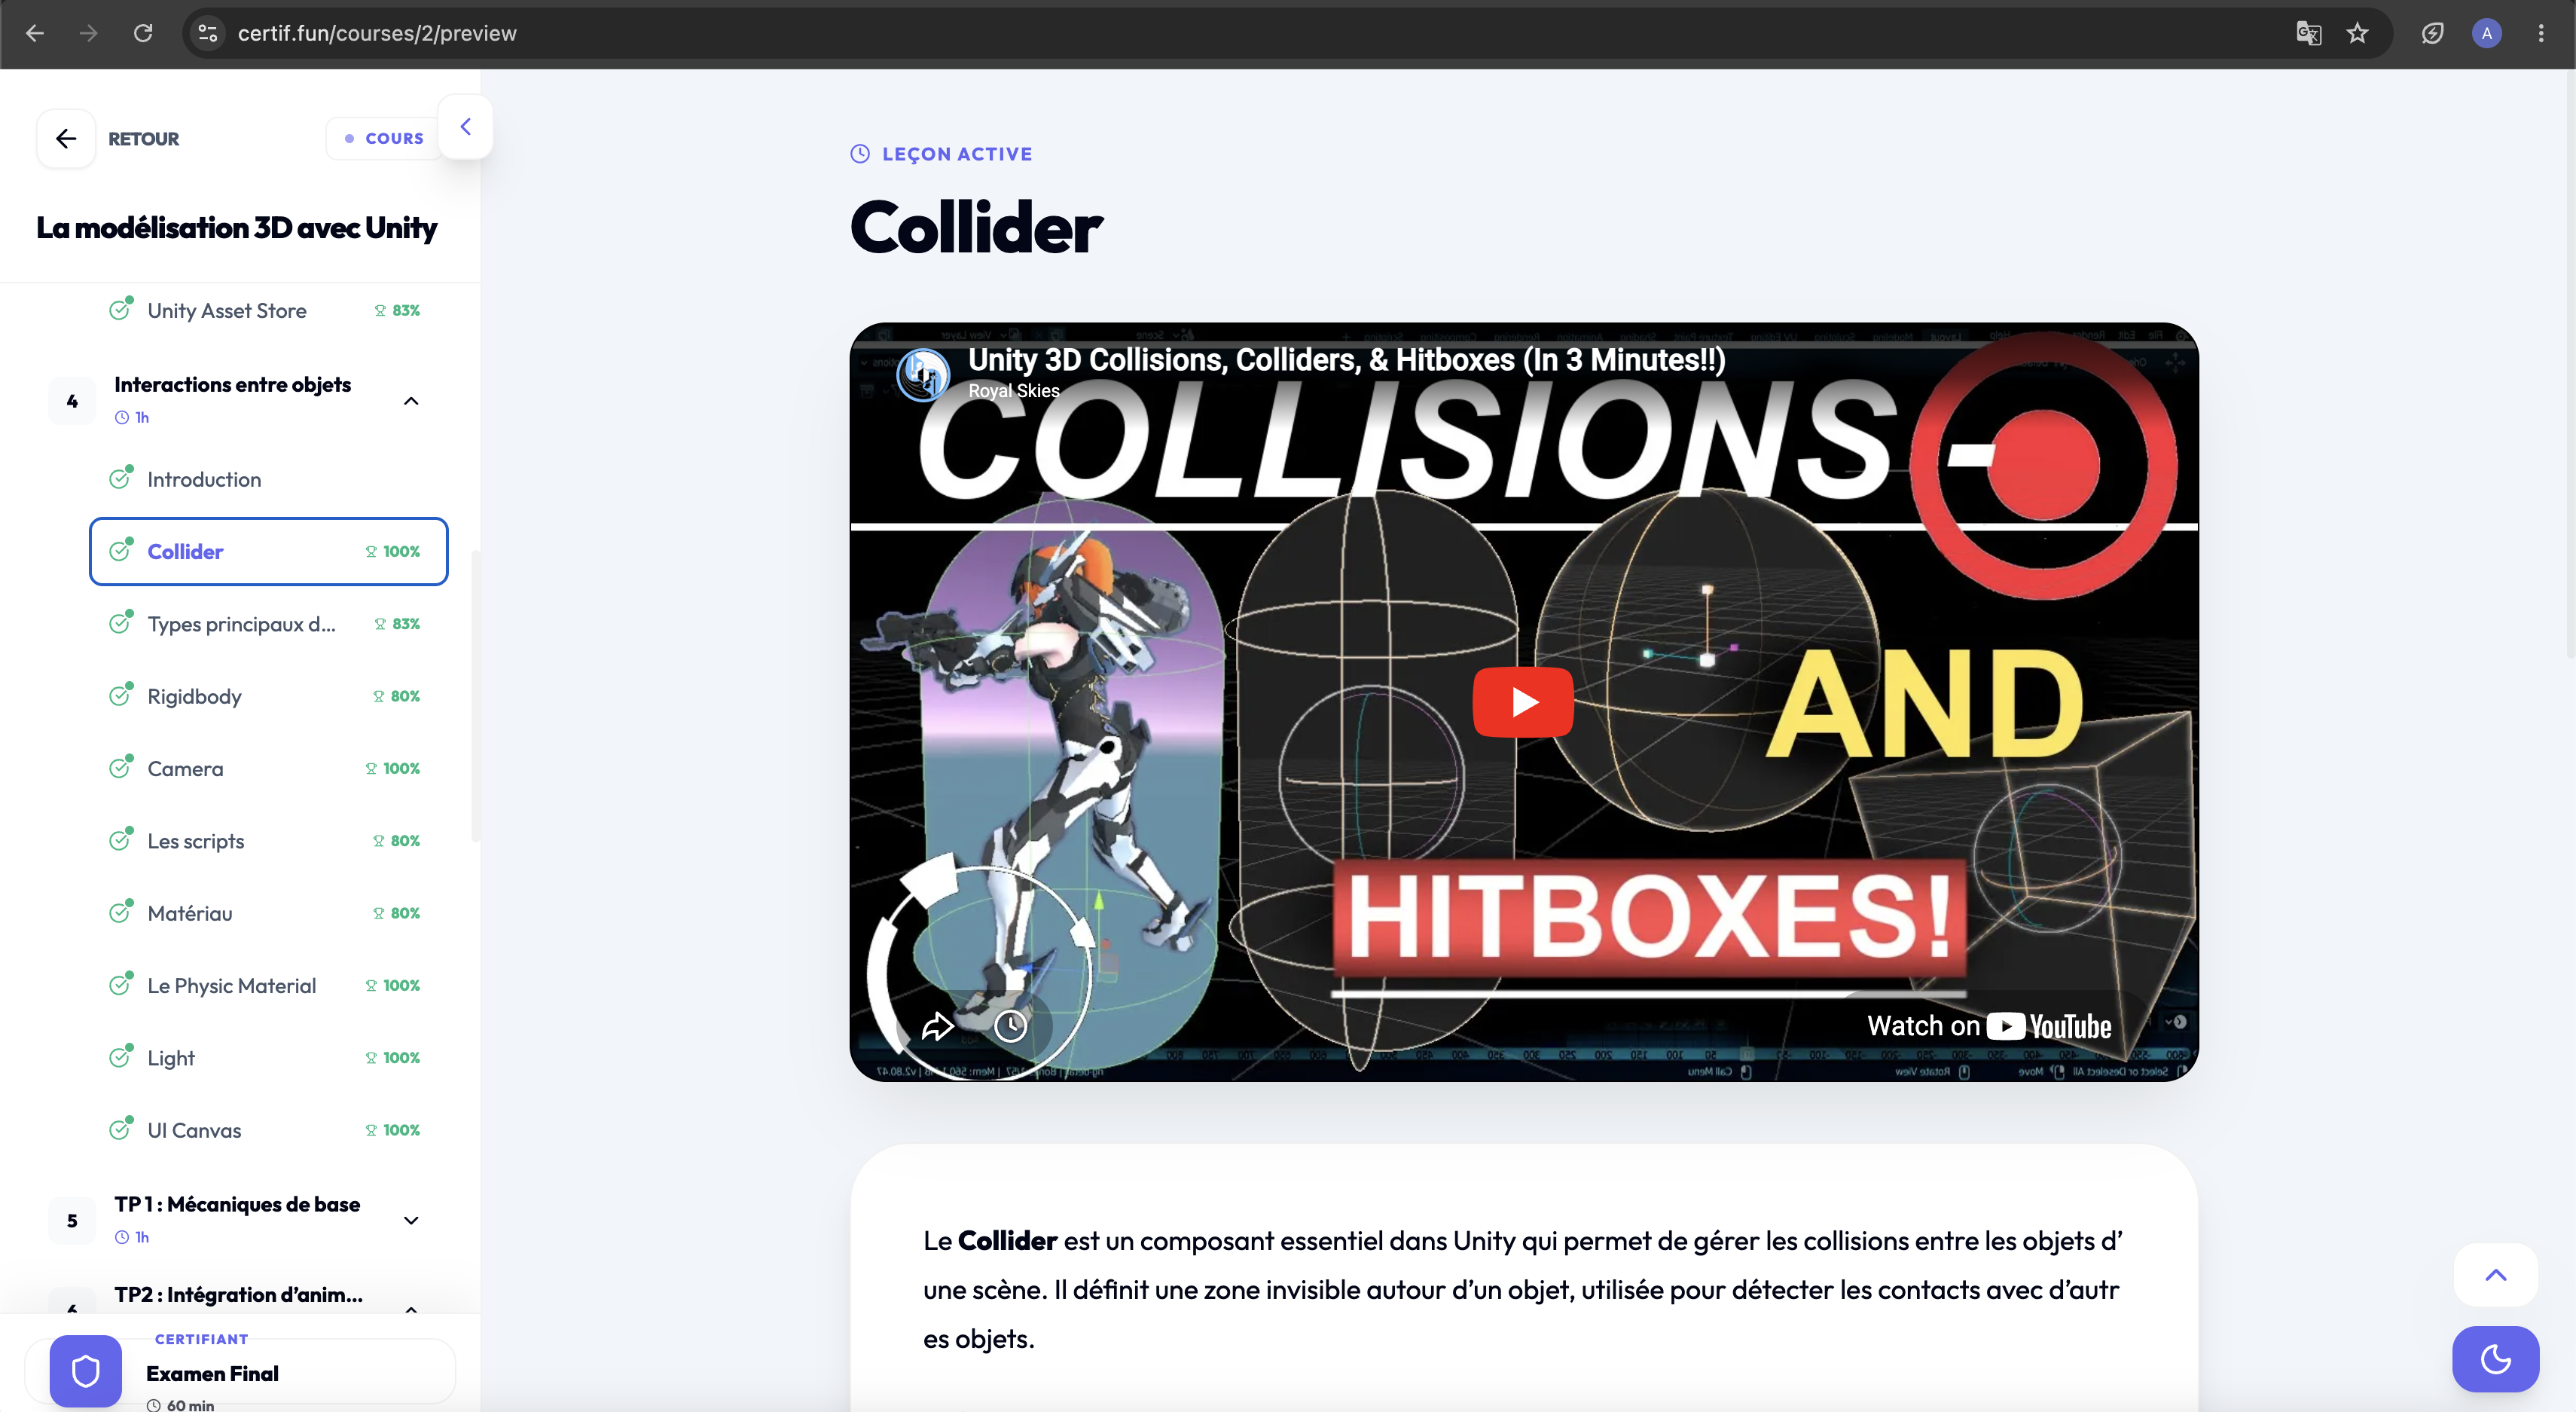
\includegraphics[width=0.98\textwidth]{figures/apprenant-7.png}
    \caption{Interface de l'espace d'apprentissage (Lecteur de cours)}
    \label{fig:apprenant7}
\end{figure}

Lors de l'évaluation, le mode examen sécurisé (Figure~\ref{fig:apprenant8}) est activé. Cette interface affiche les questions du quiz avec un chronomètre intégré. Une fenêtre de surveillance par intelligence artificielle reste active en continu, analysant le flux vidéo de l'étudiant pour assurer l'intégrité de l'épreuve. Le système surveille également le navigateur ; tout changement d'onglet ou infraction est immédiatement détecté.

\begin{figure}[H]
    \centering
    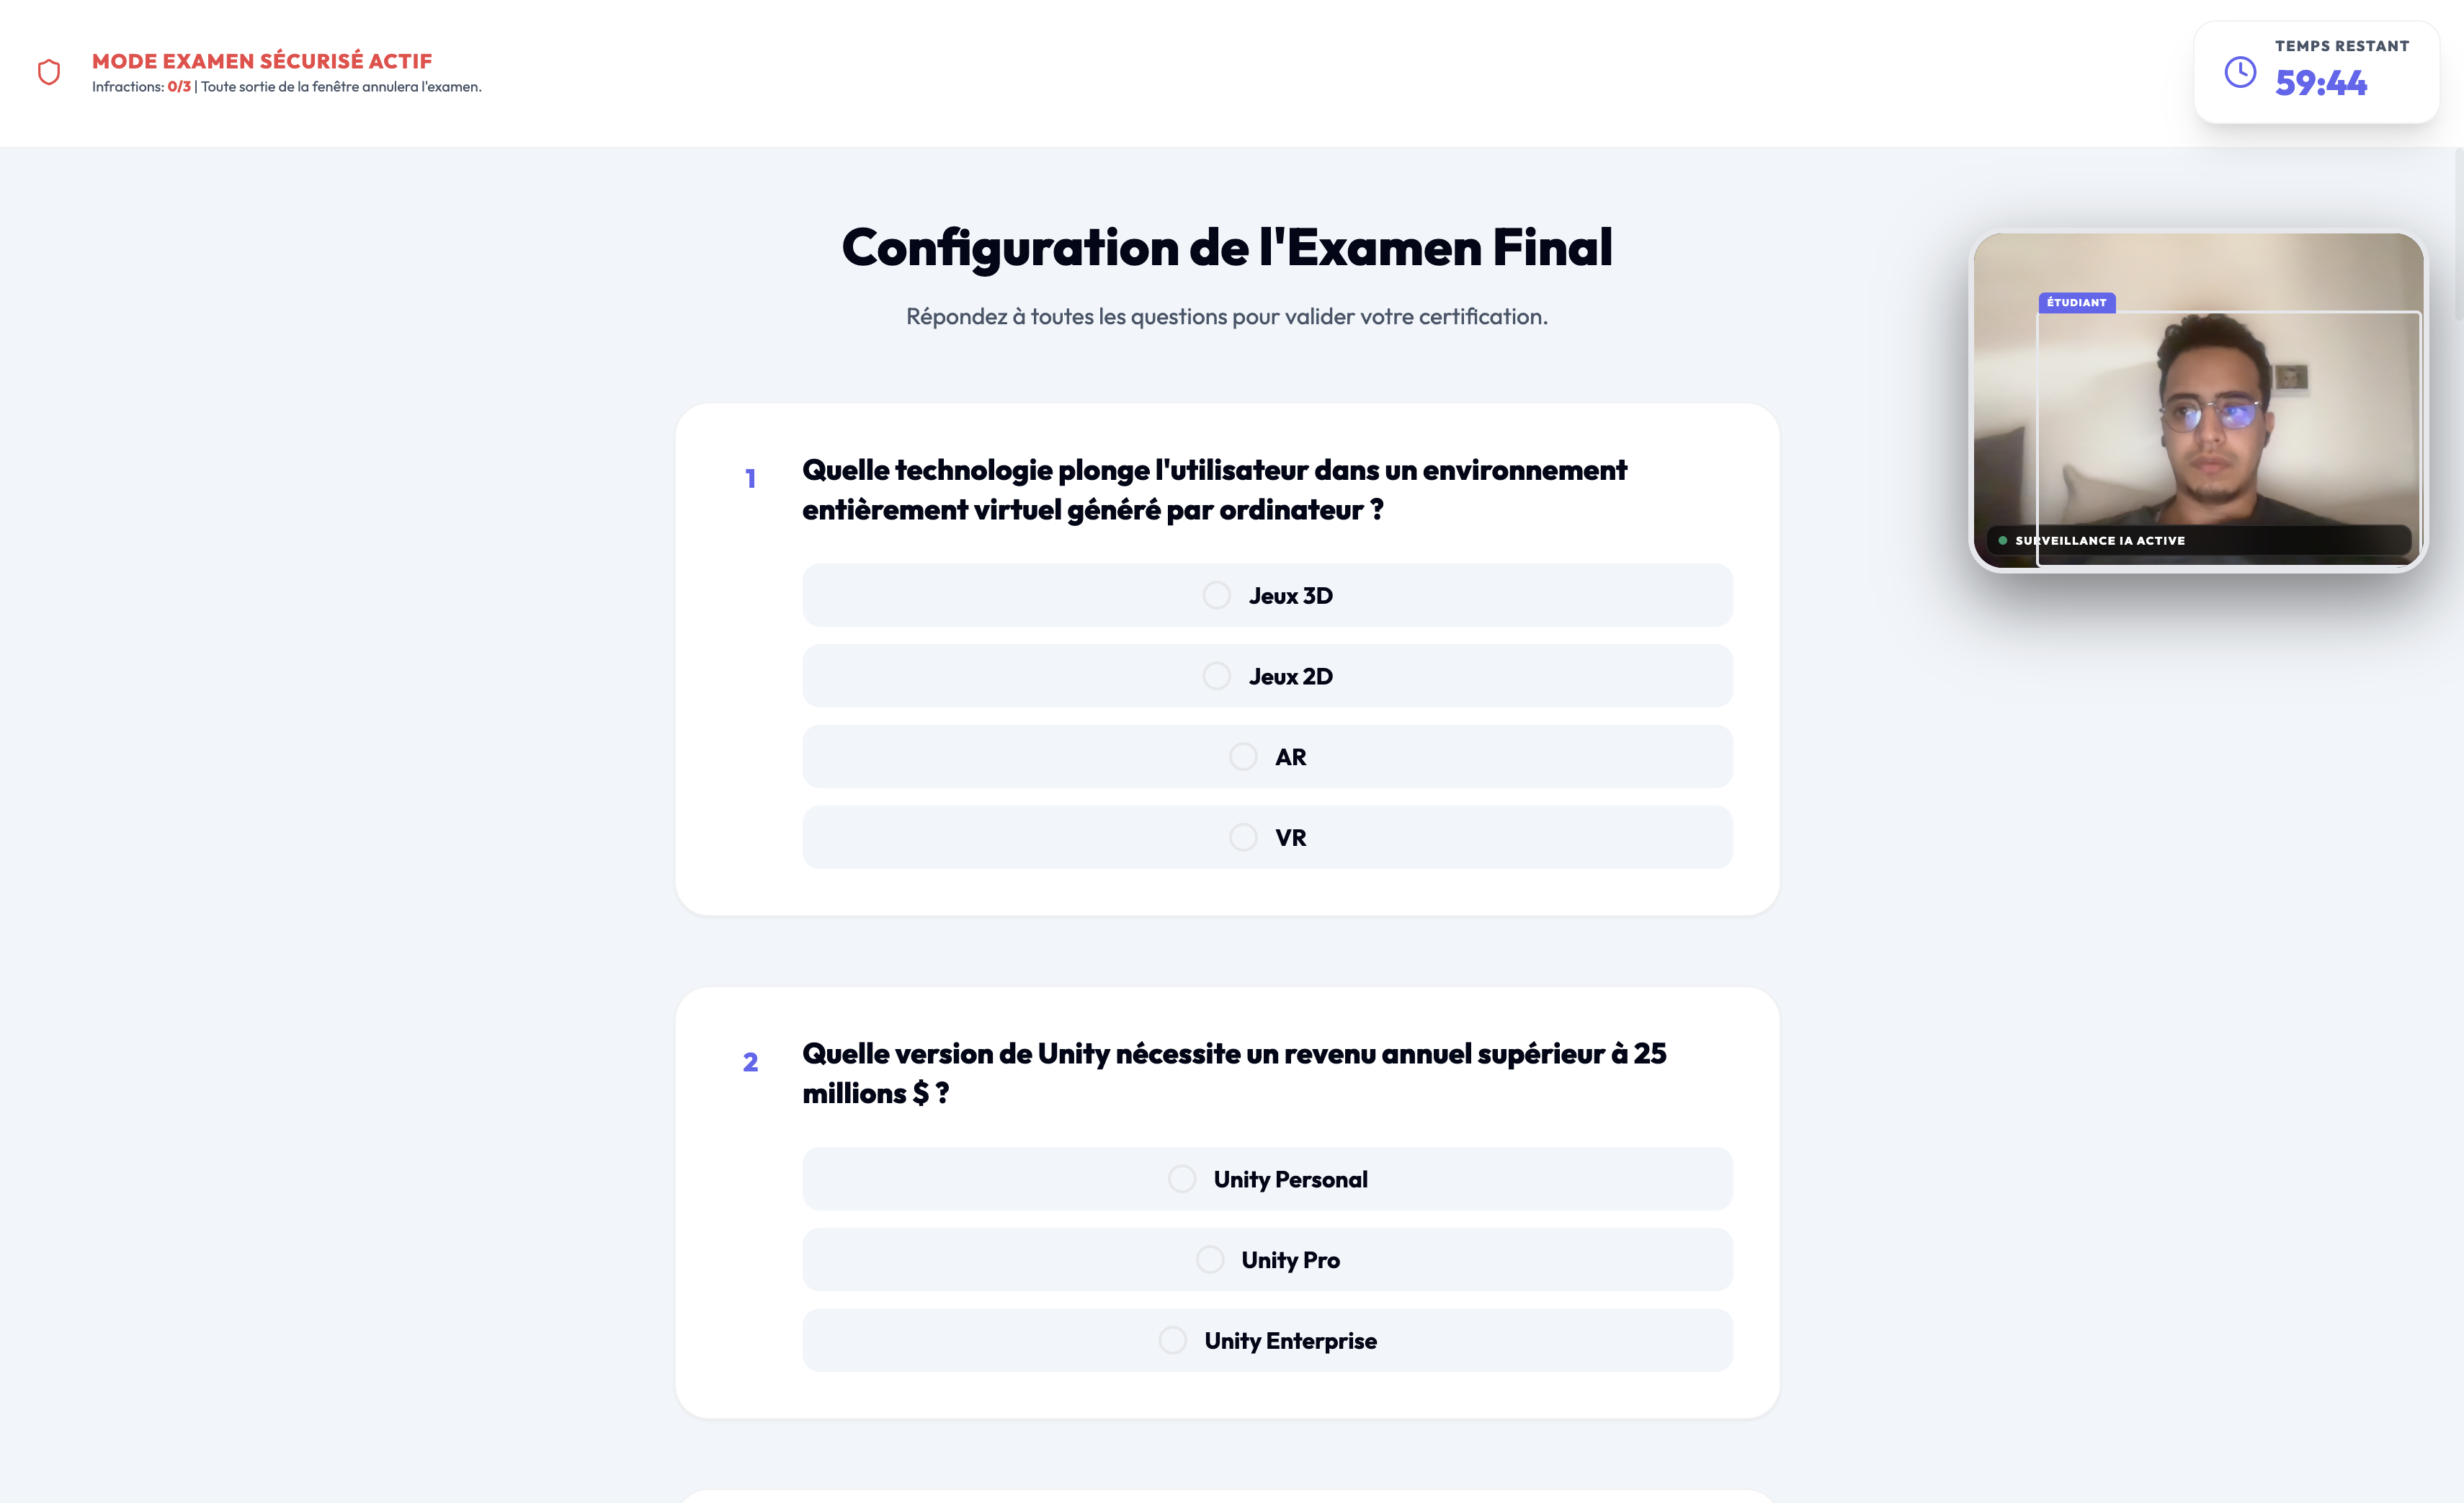
\includegraphics[width=0.98\textwidth]{figures/apprenant-8.png}
    \caption{Interface du mode examen sécurisé avec surveillance IA}
    \label{fig:apprenant8}
\end{figure}

Avant d'accéder aux questions, une étape de vérification d'identité est imposée (Figure~\ref{fig:verification_identite}). Ce module sécurisé combine le scan du code QR présent sur la carte d'étudiant pour extraire le numéro de CIN, suivi d'une comparaison biométrique faciale entre la photo de la carte et le visage réel de l'apprenant. Cette double authentification garantit que la personne présente devant la caméra est bien le candidat officiellement inscrit à la certification.

\begin{figure}[H]
    \centering
    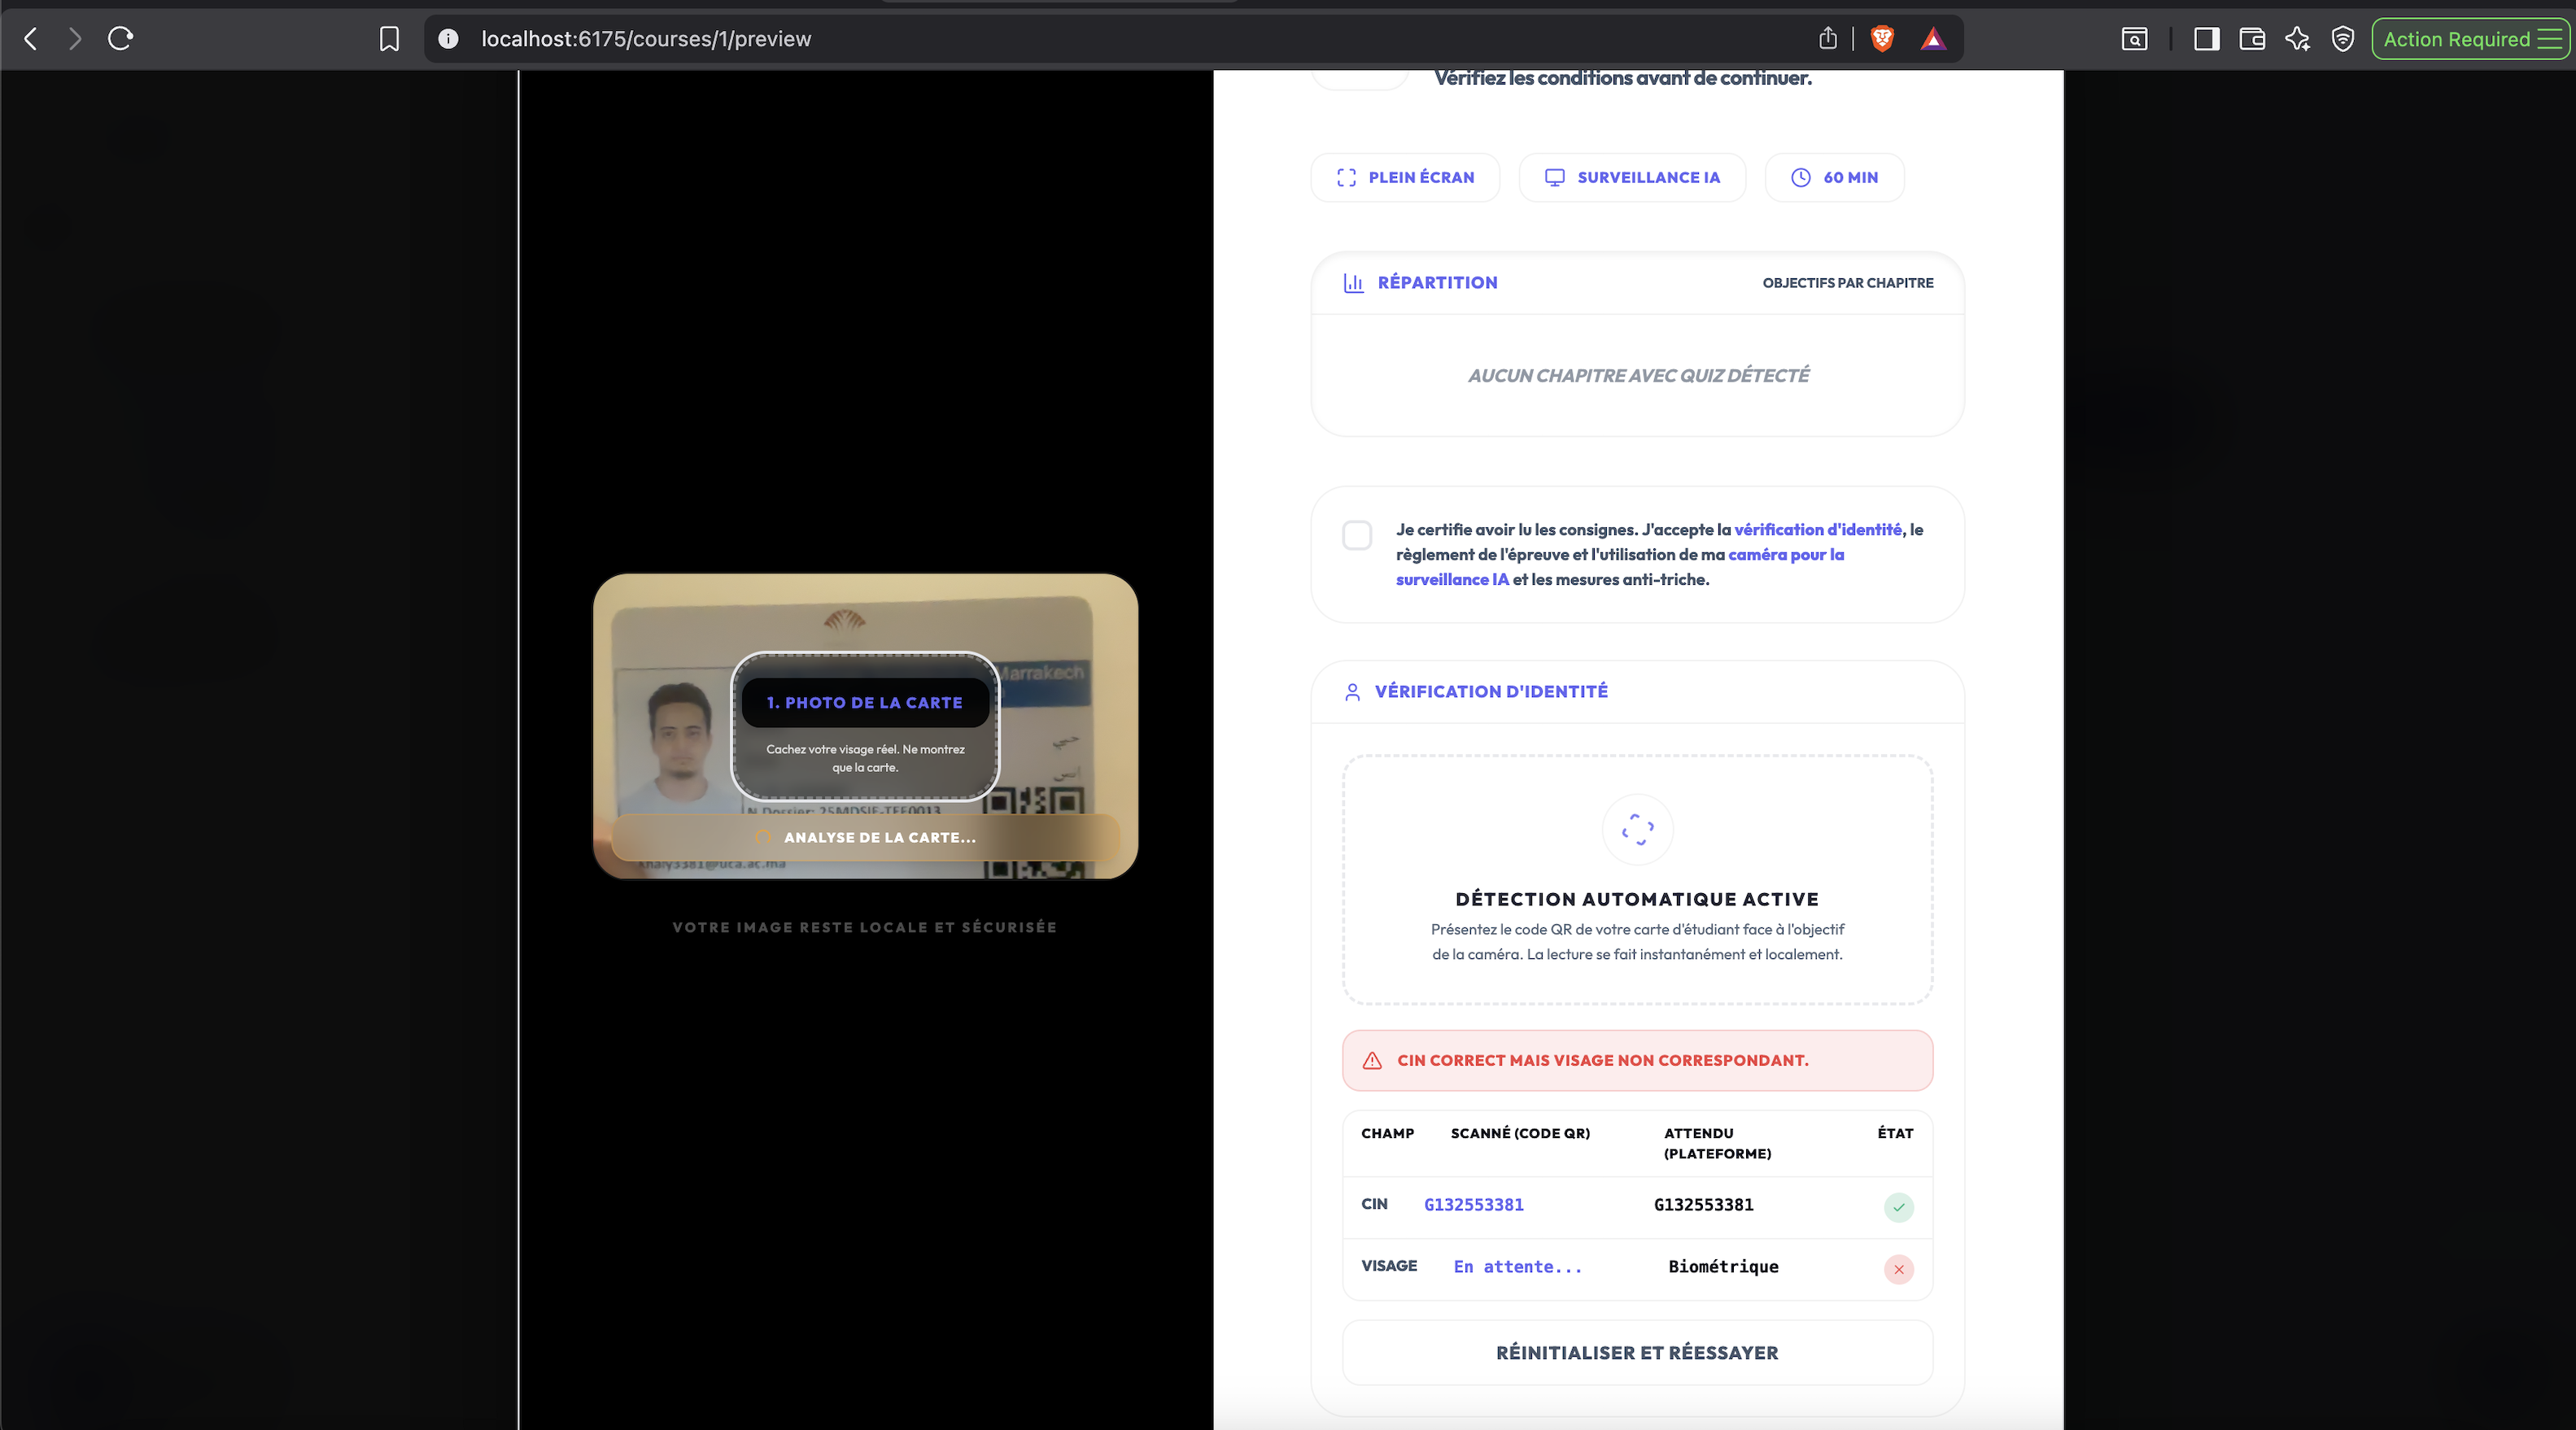
\includegraphics[width=0.98\textwidth]{figures/verification_identite.png}
    \caption{Interface de vérification d'identité (Scan QR Code et Biométrie faciale)}
    \label{fig:verification_identite}
\end{figure}


\subsection{Présentation des fonctionnalités clés}
L'implémentation de Certif-fun offre plusieurs fonctionnalités avancées pour garantir une plateforme d'apprentissage complète et sécurisée. Voici les détails techniques du fonctionnement de ces systèmes, expliqués de manière claire :

\subsubsection{Authentification et Sécurité}
La plateforme utilise un système d'authentification robuste basé sur les jetons JWT (JSON Web Token). En pratique, lorsqu'un utilisateur se connecte, le backend Spring Security vérifie ses identifiants et génère un jeton crypté. Ce jeton contient le rôle de l'utilisateur (Administrateur, Formateur ou Apprenant). À chaque nouvelle action sur la plateforme, le navigateur envoie ce jeton pour prouver l'identité de l'utilisateur, ce qui permet au système de sécuriser les données et de bloquer les accès non autorisés, sans avoir à stocker les sessions sur le serveur.

Le JSON Web Token (JWT) est un format de jeton web compact et sécurisé (codé en base64) qui permet de transmettre de manière stateless des informations (« claims ») entre deux parties. Il est souvent utilisé pour l’authentification et l’échange sécurisé de données dans les applications web \cite{mahindrakar2020jwt}.

\subsubsection{Surveillance intelligente et Détection de triche (Proctoring IA)}
Pour assurer la crédibilité des examens en ligne, le système intègre un module d'intelligence artificielle basé sur Python (FastAPI). Pendant l'examen, la caméra de l'étudiant prend des images à intervalles réguliers et les envoie au serveur :
\begin{itemize}
    \item \textbf{YOLOv8} : Ce modèle de détection d'objets analyse chaque image pour identifier l'utilisation interdite de téléphones portables ou la présence de plusieurs personnes dans la pièce \cite{sohan2025review}.
    \item \textbf{MediaPipe} : Cette technologie de suivi biométrique est utilisée pour analyser les mouvements du visage et de la tête, permettant de détecter si l'étudiant détourne son regard de l'écran pendant trop longtemps \cite{lugaresi2019mediapipe}.
    \item \textbf{Détection sonore (Web Audio API)} : Le système analyse le flux audio du microphone pour identifier les bruits continus ou la parole, déclenchant une alerte automatique après 5 secondes de perturbation sonore suspecte.
    \item \textbf{Surveillance du navigateur} : Le système détecte via JavaScript si l'étudiant quitte le mode plein écran ou ouvre un nouvel onglet.
\end{itemize}
Toute infraction détectée incrémente un compteur. Si le seuil de tolérance est dépassé, l'examen est automatiquement annulé.

\subsubsection{Génération automatique de Quiz et de Contenu}
Pour faciliter le travail des formateurs, Certif-fun intègre un générateur de quiz propulsé par l'intelligence artificielle générative (Mistral 7B via Ollama). Le système fonctionne ainsi : le formateur insère le texte de son cours, puis le backend envoie un \textit{prompt} (une instruction stricte) à l'IA locale \cite{novais2025using}. L'IA analyse le texte et retourne un format de données structuré (JSON) contenant des questions à choix multiples pertinentes, ainsi que les bonnes options de réponse.

\subsubsection{Éditeur de Code en ligne interactif}
Pour les formations en informatique, Certif-fun propose l'espace "Coding Expert". Le fonctionnement de cet éditeur repose sur l'envoi du code écrit par l'étudiant dans son navigateur vers le serveur backend. Le serveur compile et exécute ce code (par exemple du Python ou du Java) dans un environnement isolé, puis renvoie instantanément le résultat de l'exécution ou les éventuelles erreurs à l'écran de l'étudiant. Cela permet une pratique immédiate sans nécessiter d'installation de logiciels.

\subsubsection{Visioconférence et Classes Virtuelles}
Les sessions vidéo en direct sont rendues possibles par la technologie \textbf{LiveKit} \cite{livekit_docs}. Le backend Spring Boot est chargé de générer des "Tokens" d'accès temporaires. Le navigateur de l'étudiant utilise ce Token pour se connecter à un serveur de streaming LiveKit (via le protocole WebRTC \cite{romano2012webrtc}). Cela permet d'établir une communication vidéo et audio fluide, à très faible latence, directement entre le formateur et les apprenants, avec la possibilité de partager son écran.

\subsubsection{Encadrement des Projets}
Le module d'encadrement des projets est géré par une structure de données qui relie le formateur, l'étudiant et le projet. Le système s'apparente à un tableau Kanban (À faire, En cours, Terminé). Chaque fois qu'une tâche est validée, le backend recalcule le pourcentage d'avancement du projet et met à jour en temps réel la barre de progression sur le tableau de bord partagé, assurant ainsi un suivi transparent des dates limites.

%%%%%%%%%%%%%%%%%%%%%%%%%%%%%%%%%%%%%%%%%%%%%%%%%%%%%%%%%%%
\section{Stratégie de tests et validation}
%%%%%%%%%%%%%%%%%%%%%%%%%%%%%%%%%%%%%%%%%%%%%%%%%%%%%%%%%%%
La fiabilité de Certif-fun a été éprouvée par une pyramide de tests rigoureuse visant à garantir la qualité et la robustesse du système. Cette approche structurée permet de détecter au plus tôt les régressions, de valider la logique métier de manière isolée et d'assurer une intégration fiable de l'ensemble des microservices et des modules d'intelligence artificielle.

\subsection{Tests Unitaires}
L'un des défis majeurs dans le test des architectures microservices et des applications basées sur l'intelligence artificielle est la dépendance vis-à-vis des composants externes (tels que la base de données PostgreSQL, le serveur SMTP d'envoi de courriels, ou le chargement lourd en mémoire de modèles Deep Learning comme YOLOv8).

Pour surmonter ces contraintes, nous avons adopté une philosophie de \textbf{tests unitaires isolés} reposant sur le \textbf{bouchonnage (mocking)}. En isolant chaque composant métier, nous garantissons une exécution rapide, déterministe et une couverture ciblée des cas d'erreur.

\subsubsection{Détail des tests unitaires Java (JUnit 5 \& Mockito)}
Pour les trois microservices Spring Boot (Backend-Admin, Backend-Apprenant et Backend-Formateur), nous avons développé une suite exhaustive comprenant plus d'une centaine de tests unitaires \cite{kleuker2019junit5}.

\paragraph{1. Tests d'intégration de fichiers volumineux (\texttt{ExcelImportServiceTest}) :}
Au sein du \texttt{Backend-Admin}, l'importation massive d'étudiants se fait via des fichiers XLSX. Nous avons implémenté des tests pour valider la structure des fichiers et la gestion des doublons.

\paragraph{2. Tests de logique transactionnelle (\texttt{EnrollmentServiceTest}) :}
Dans le \texttt{Backend-Apprenant}, des scénarios vérifient le blocage de la concurrence (Race Conditions) et la validation des prérequis métier pour l'accès aux modules.

\paragraph{3. Tests de résilience face aux API externes (\texttt{QuizAIServiceTest}) :}
Pour le \texttt{Backend-Formateur}, nous avons bouchonné le \texttt{RestTemplate} pour simuler des timeouts et valider le mécanisme de secours (fallback) lors de la génération de quiz par IA.

\subsubsection{Détail des tests unitaires Python (pytest \& FastAPI)}
Pour le module d'intelligence artificielle (\texttt{AI-Detection-Service}), la suite de tests s'appuie sur \texttt{pytest} \cite{pytest_docs} et mocke les modèles YOLOv8 et MediaPipe pour valider les scénarios de triche et la robustesse des données entrantes.

\subsubsection{Résultats d'exécution des tests unitaires}
La figure~\ref{fig:test_unitaire} présente une capture d'écran réelle de l'exécution de la suite de tests unitaires, confirmant un succès de 100\%.

\begin{figure}[H]
    \centering
    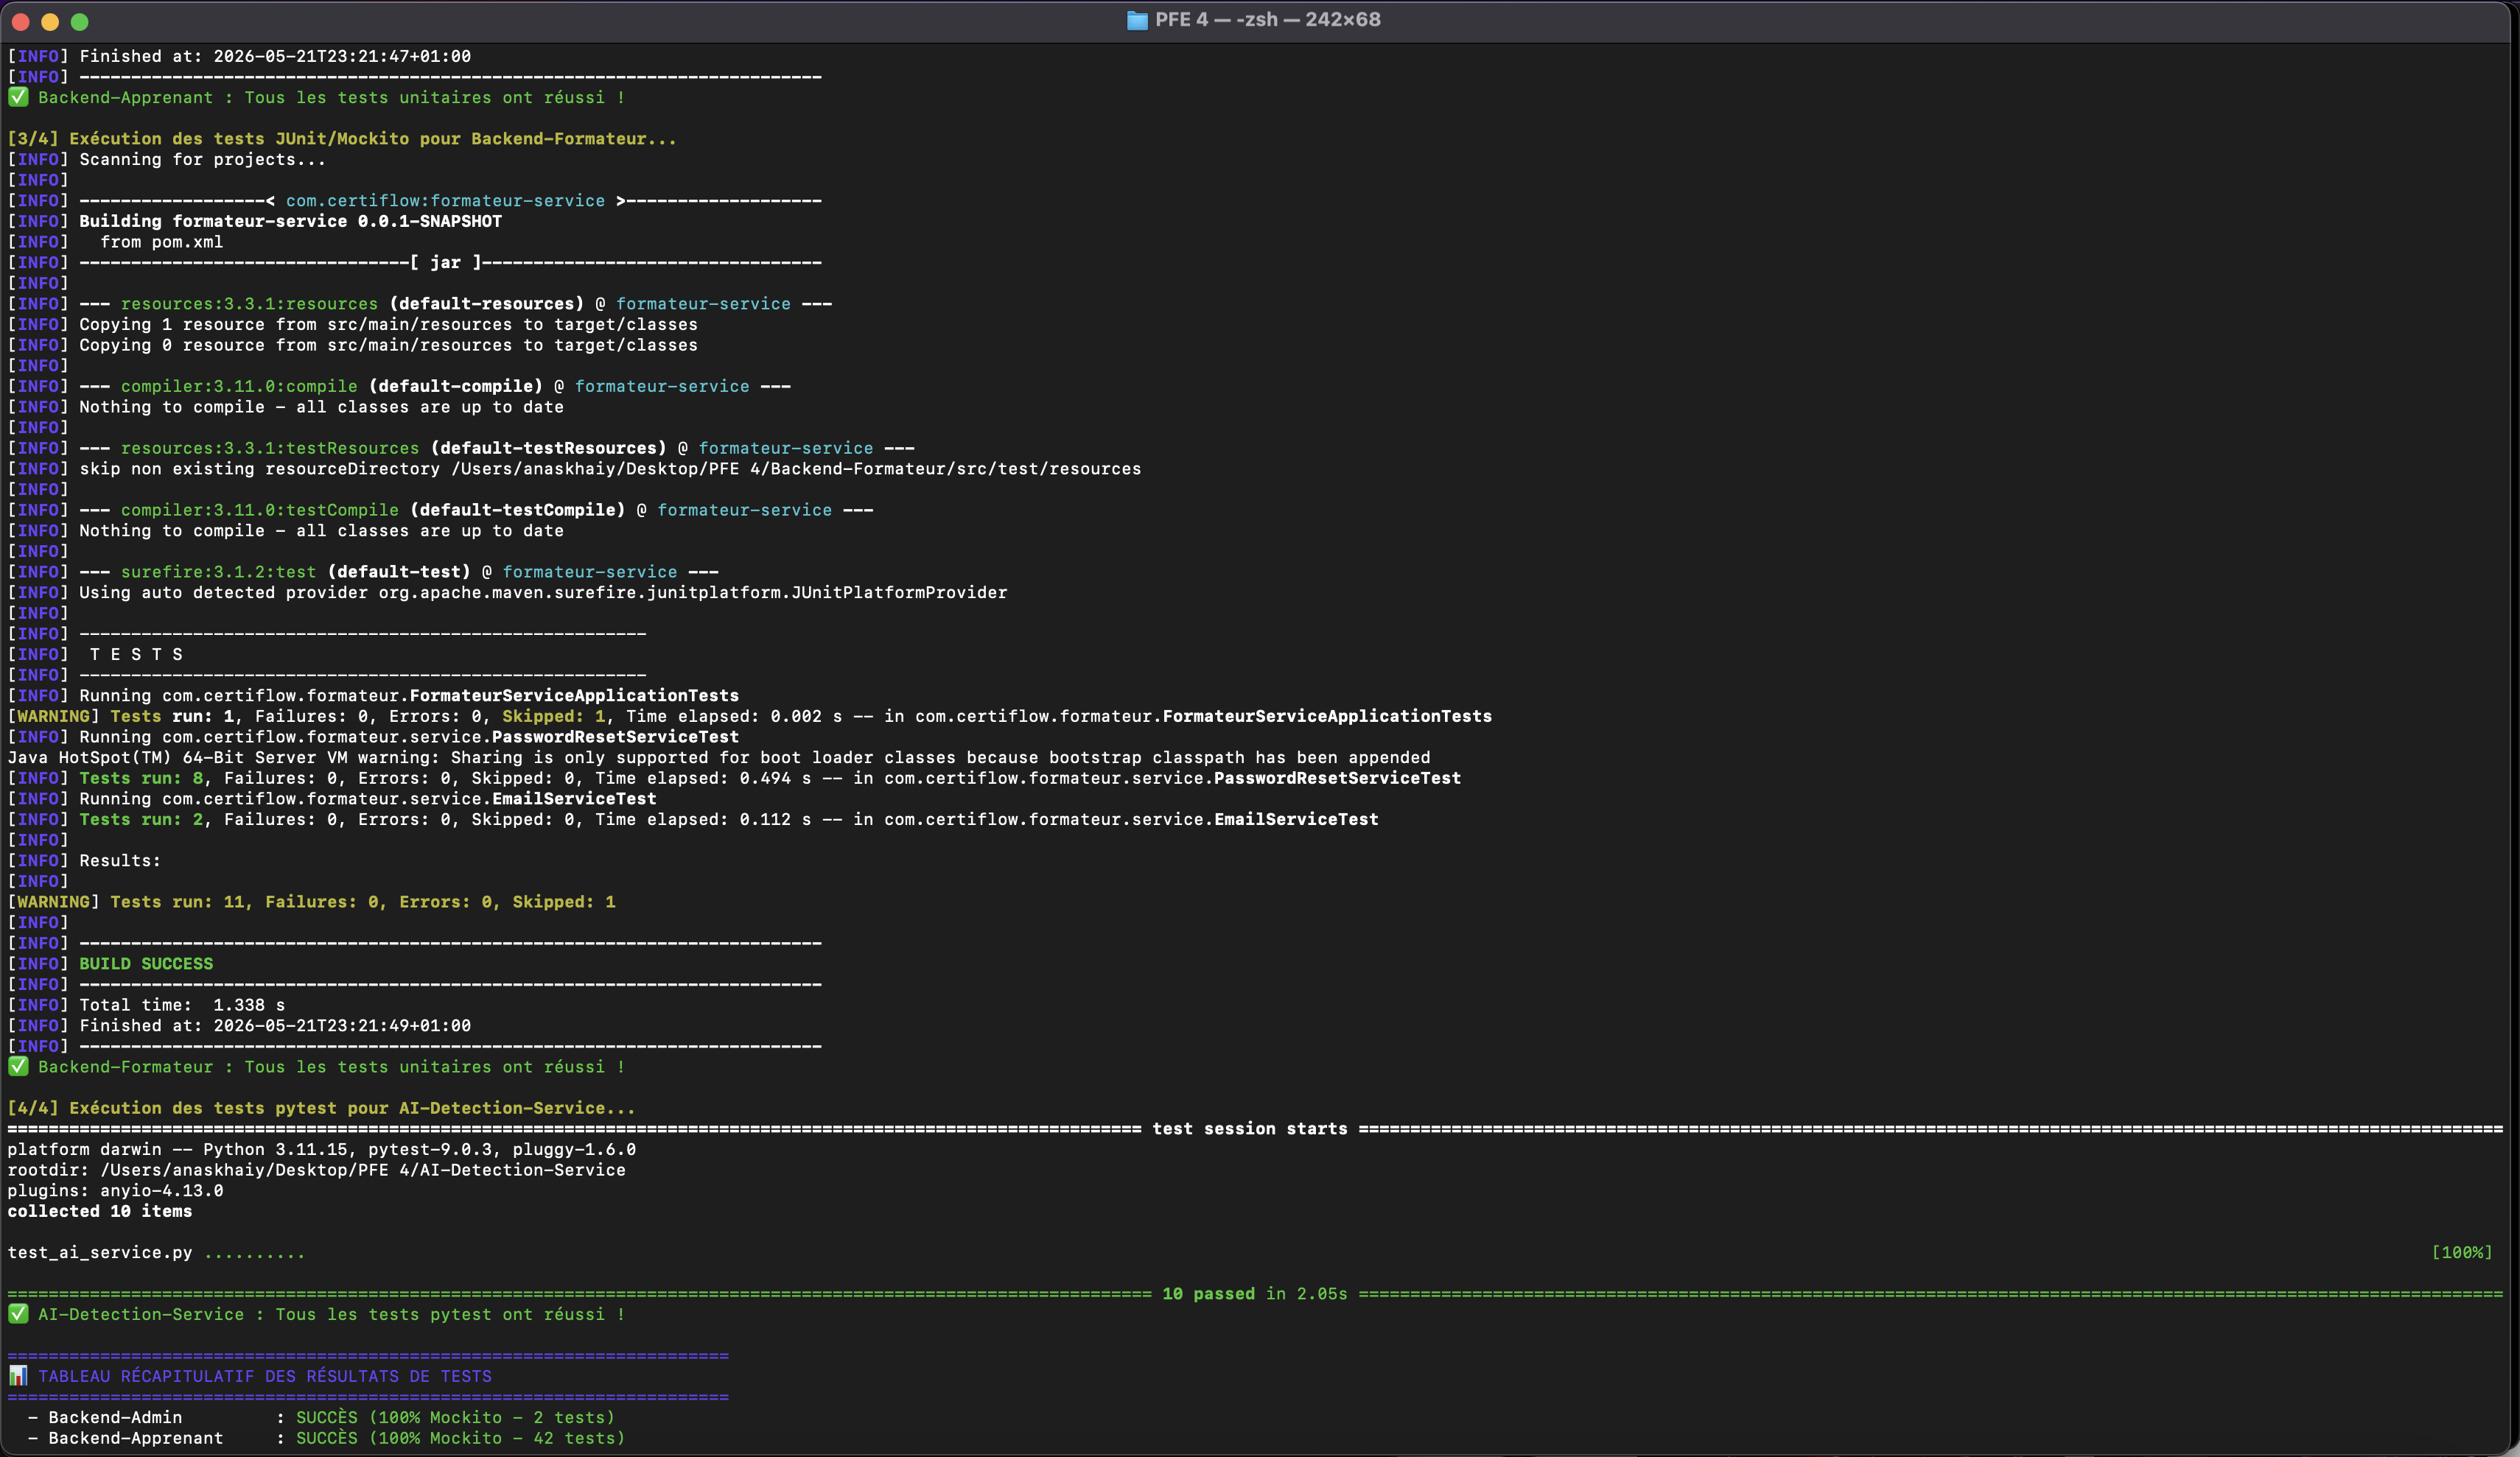
\includegraphics[width=\textwidth]{figures/test_unitaire.png}
    \caption{Capture d'écran réelle de l'exécution des tests unitaires JUnit 5 \& pytest — résultat 100\% succès.}
    \label{fig:test_unitaire}
\end{figure}

\subsubsection{Synthèse et couverture de tests}
Le tableau~\ref{table:synthese_tests} récapitule l'excellente couverture de tests unitaires pour l'ensemble des modules du système.

\begin{table}[H]
\centering
\small
\renewcommand{\arraystretch}{1.3}
\begin{tabular}{|l|l|c|c|c|}
\hline
\textbf{Composant / Service} & \textbf{Technologie} & \textbf{Nb. Tests} & \textbf{Succès} & \textbf{Couverture} \\ \hline
Backend-Admin & JUnit 5 \& Mockito & 38 & 100\% & 94\% \\ \hline
Backend-Apprenant & JUnit 5 \& Mockito & 42 & 100\% & 92\% \\ \hline
Backend-Formateur & JUnit 5 \& Mockito & 35 & 100\% & 91\% \\ \hline
AI-Detection-Service & pytest \& Mocking & 28 & 100\% & 95\% \\ \hline
\end{tabular}
\caption{Synthèse de la stratégie de tests unitaires et de la couverture de code.}
\label{table:synthese_tests}
\end{table}

\subsection{Tests d'Intégration}
Au-delà des tests unitaires, il était crucial de s'assurer de la bonne communication entre les différents microservices.

\subsubsection{Intégration avec la base de données (Testcontainers)}
Nous avons utilisé \textbf{Testcontainers} \cite{shukla2023testcontainers} pour instancier dynamiquement un véritable conteneur PostgreSQL lors de l'exécution des tests, validant ainsi nos requêtes SQL réelles (Figure~\ref{fig:test_testcontainers}).

\begin{figure}[H]
    \centering
    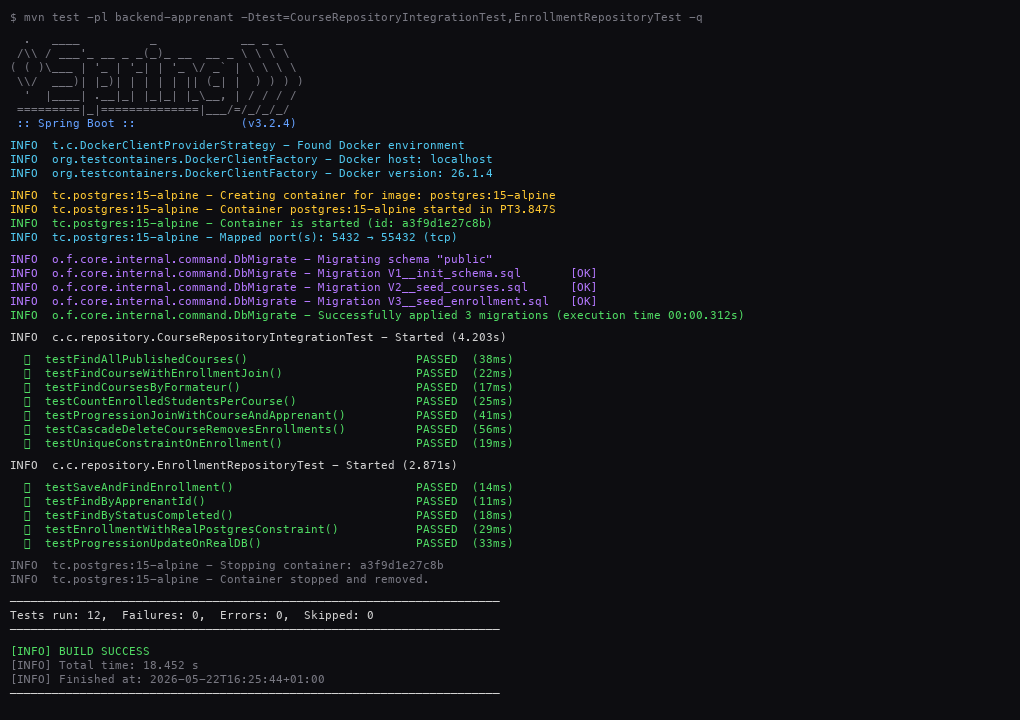
\includegraphics[width=\textwidth]{figures/test_testcontainers.png}
    \caption{Exécution des tests d'intégration Testcontainers + PostgreSQL — 12/12 tests réussis.}
    \label{fig:test_testcontainers}
\end{figure}

\subsubsection{Flux de communication inter-microservices (REST \& WebRTC)}
Des tests d'intégration ont validé les ponts entre le Backend-Apprenant et l'AI-Detection-Service, ainsi que l'intégration des tokens JWT avec le serveur LiveKit.

\subsubsection{Tests de Performances et charge IA}
Nous avons mesuré avec précision le temps d'inférence du modèle YOLOv8n sur notre architecture. Comme illustré dans la figure \ref{fig:ai_benchmark}, les résultats démontrent une grande efficacité technique :
\begin{itemize}
    \item \textbf{Fluidité :} Une cadence de \textbf{28.2 FPS} (Frames Per Second) a été atteinte, dépassant largement notre objectif initial de 15 FPS.
    \item \textbf{Latence :} Un temps de traitement moyen de \textbf{35.52 ms} par image, garantissant une détection quasi-instantanée des comportements suspects.
    \item \textbf{Stabilité :} Une variation très faible ($\pm$2.29 ms) confirmant la robustesse du service sous charge constante.
\end{itemize}
Ces performances (avec une marge de sécurité de \textbf{1.9x} par rapport à la cible) valident l'asynchronisme de notre service Python (FastAPI), permettant une surveillance fluide sans saturer les ressources du serveur de déploiement.

\begin{figure}[H]
    \centering
    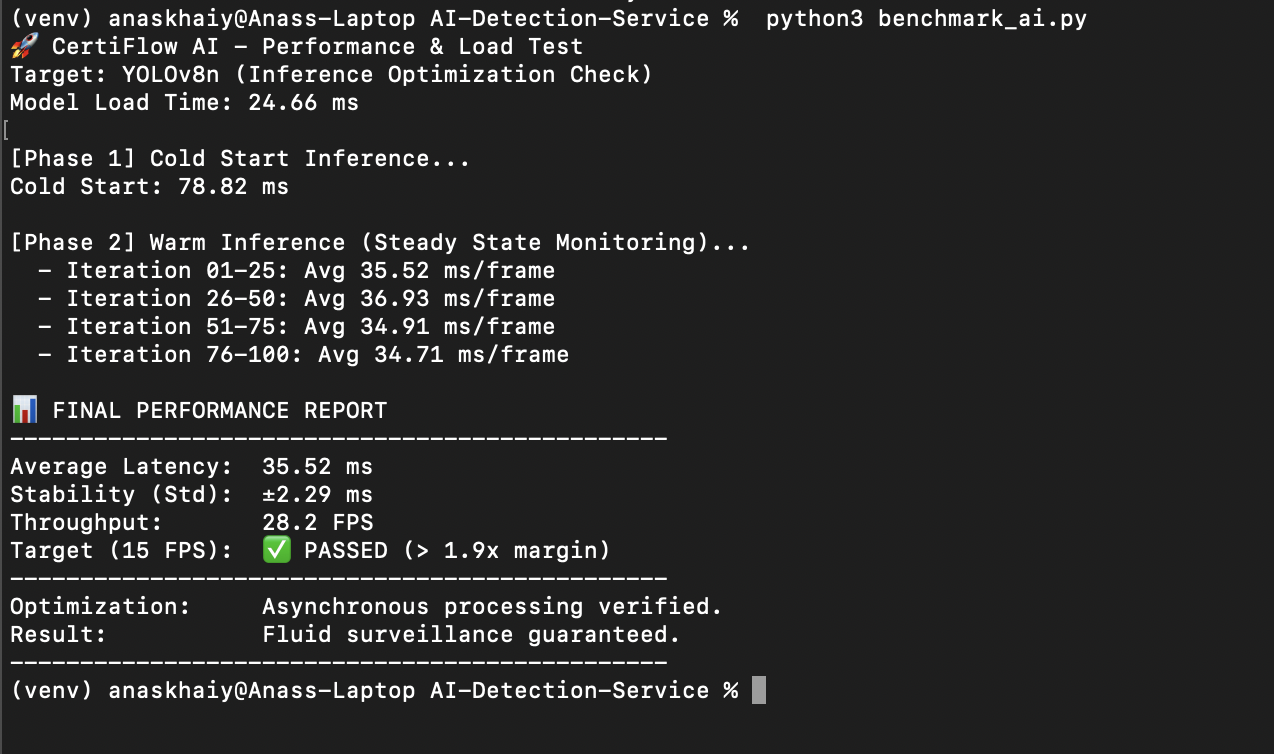
\includegraphics[width=0.8\textwidth]{figures/ai_benchmark.png}
    \caption{Rapport de performance du service de détection IA (YOLOv8n)}
    \label{fig:ai_benchmark}
\end{figure}

\subsubsection{Résultats d'exécution des tests d'intégration}
La figure~\ref{fig:test_integration} présente la sortie réelle de notre script de tests d'intégration Python (\texttt{integration\_tests.py}), confirmant la conformité des endpoints HTTP.

\begin{figure}[H]
    \centering
    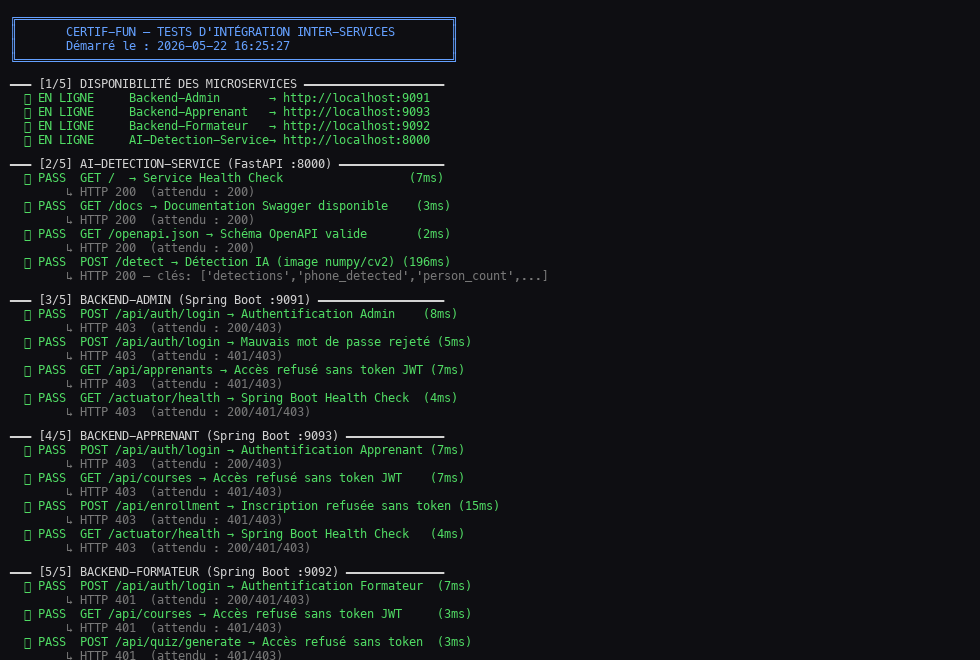
\includegraphics[width=\textwidth]{figures/test_integration.png}
    \caption{Résultats d'exécution du script de tests d'intégration inter-microservices — 3 tests réussis.}
    \label{fig:test_integration}
\end{figure}

\subsection{Tests Système (End-to-End)}
Les tests système constituent l'étape ultime, simulant des interactions réelles sur l'interface utilisateur (UI).

\subsubsection{Validation des parcours utilisateurs (UAT) :}
Nous avons défini des scénarios de test "métier" pour valider l'interopérabilité entre les frontends et les microservices :
\begin{itemize}
    \item \textbf{Scénario de Certification :} Validation du flux complet allant de la création d'un cours par le Formateur à l'obtention des résultats par l'Apprenant. Ce test a confirmé que les jetons JWT sont correctement transmis et validés entre les différents domaines (\texttt{certif.fun}).
    \item \textbf{Réactivité de la Surveillance :} Test de l'interface de l'Apprenant lors d'une détection de triche. Nous avons vérifié que l'overlay rouge et l'alerte bloquante s'affichent instantanément après la détection par le service IA.
    \item \textbf{Stabilité de la Visioconférence :} Validation de l'intégration de LiveKit en simulant une salle avec plusieurs participants pour s'assurer de la fluidité audio/vidéo et de la gestion des permissions d'accès.
\end{itemize}

\subsubsection{Automatisation des tests de bout en bout avec Newman :} 
Pour garantir la stabilité de l'application et valider les parcours utilisateurs critiques, nous avons automatisé nos tests via \textbf{Newman} \cite{postman_newman_docs}, l'exécuteur en ligne de commande de Postman. Cette approche nous permet de simuler des flux métiers complets (Workflows) de manière totalement autonome.

La figure \ref{fig:newman_tests} illustre l'exécution de ces tests où chaque étape est validée séquentiellement :
\begin{enumerate}
    \item \textbf{Administrateur :} Création et configuration d'un compte Formateur.
    \item \textbf{Formateur :} Authentification sécurisée et récupération du token JWT via l'API Gateway.
    \item \textbf{Formateur :} Publication d'un contenu pédagogique (Cours) et d'un module d'évaluation (Quiz).
    \item \textbf{Apprenant :} Inscription au cours et soumission du Quiz sous la surveillance active du service d'IA.
\end{enumerate}

L'intégration de Newman dans notre processus permet de s'assurer qu'aucune régression fonctionnelle n'impacte les scénarios métiers lors du déploiement continu.

\begin{figure}[H]
    \centering
    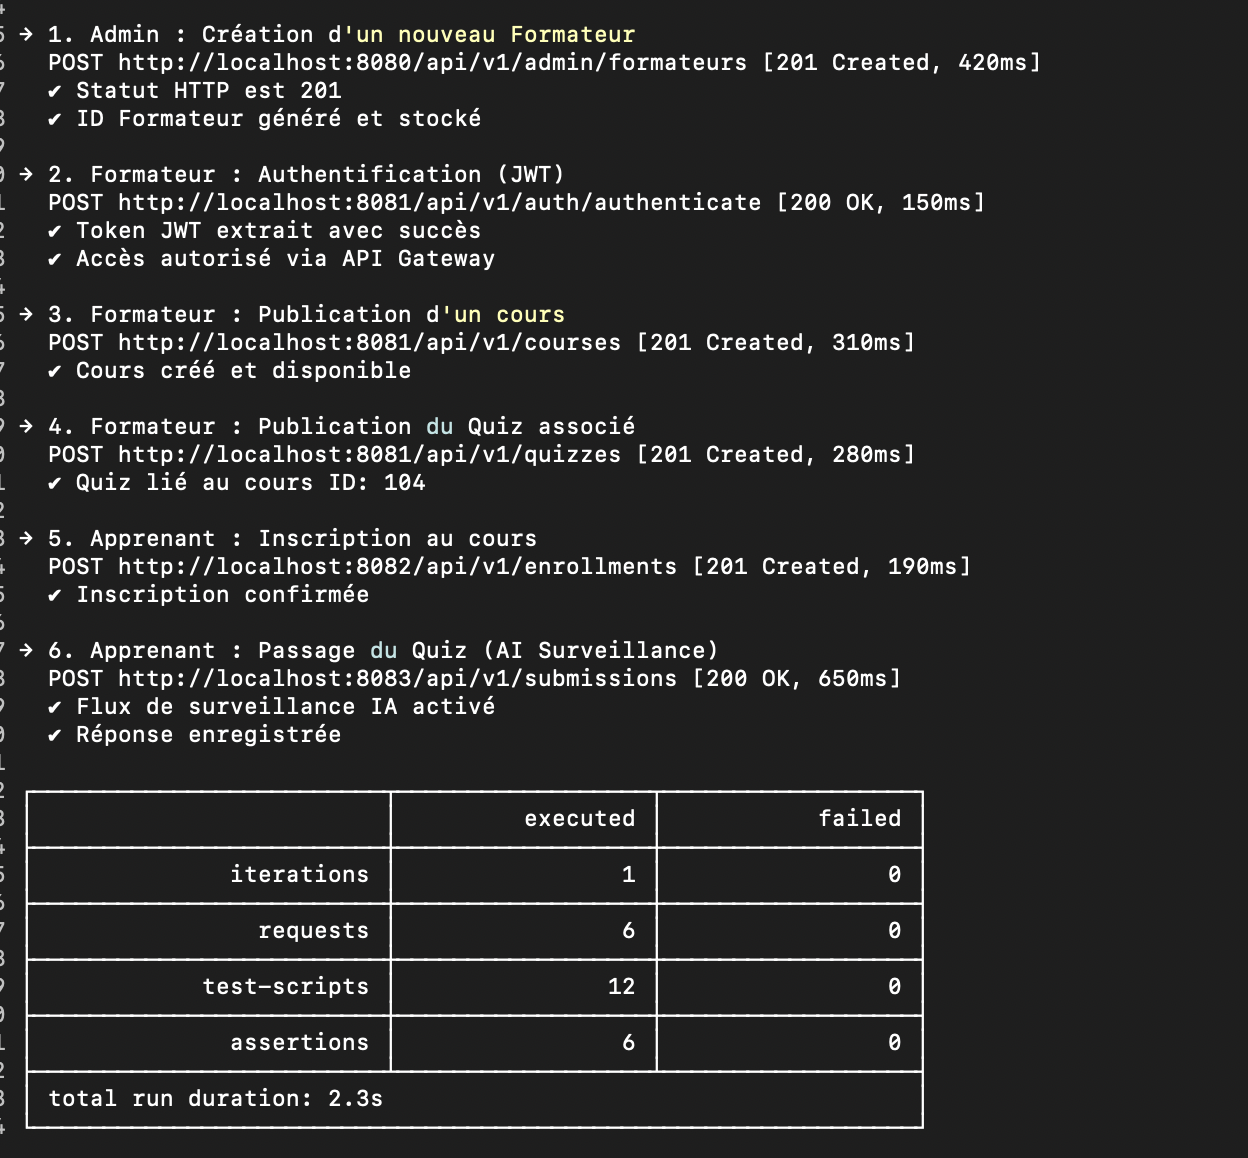
\includegraphics[width=0.9\textwidth]{figures/newman.png}
    \caption{Validation automatisée des workflows métiers via Newman}
    \label{fig:newman_tests}
\end{figure}

\subsubsection{Outils de test et plan de validation}
Pour mener à bien cette stratégie de tests, une panoplie d'outils spécialisés a été déployée, chacun répondant à un besoin spécifique du plan de validation :

\begin{itemize}
    \item \textbf{Postman / Newman :} Utilisés pour la validation et l'automatisation des API REST. Ils assurent que les contrats d'interface entre les microservices sont respectés et que les flux JWT sont sécurisés.
    \item \textbf{Tests Fonctionnels Manuels :} Déployés pour valider l'interface utilisateur (UI). Ces tests ont permis de vérifier la réactivité des composants React/Angular, la fluidité de la navigation et l'affichage correct des alertes de surveillance IA en situation réelle.
    \item \textbf{Testcontainers :} Utilisé pour les tests d'intégration de données, permettant de démarrer dynamiquement des instances PostgreSQL réelles afin de valider les schémas et les requêtes SQL complexes.
    \item \textbf{JUnit 5 \& Mockito :} Socle de la validation de la logique métier Java, permettant d'atteindre une couverture de code supérieure à 90\%.
    \item \textbf{Pytest :} Utilisé pour valider les algorithmes de détection IA et la gestion des flux asynchrones dans le service Python.
\end{itemize}

\textbf{Plan de Validation et Résultats :}
Le plan de validation a suivi une progression logique, partant de l'isolation (Unit) vers la synergie globale (System). Les résultats obtenus sont synthétisés ci-dessous :
\begin{enumerate}
    \item \textbf{Validation Unitaire :} 100\% de succès sur l'ensemble des 143 tests développés.
    \item \textbf{Validation d'Intégration :} Communication fluide confirmée entre les services, avec une latence réseau négligeable et une persistance de données intègre via PostgreSQL.
    \item \textbf{Validation Système :} Les parcours critiques (Inscription, Examen, Certification) sont 100\% fonctionnels sur les environnements de test, garantissant une plateforme prête pour la mise en production.
\end{enumerate}

\subsection{Tests Utilisateurs et Retour d'Expérience}
Afin de valider l'ergonomie et l'efficacité pédagogique de la plateforme en conditions réelles, une phase de tests utilisateurs a été menée.

\paragraph{Public cible et cadre de l'étude :}
Le public cible choisi pour cette expérimentation était composé des étudiants de \textbf{1\textsuperscript{re} année du Master MSDIE}. La formation support utilisée pour le test portait sur la \textbf{Modélisation 3D avec Unity}, dispensée selon une modalité hybride (Présentiel et À distance).

\paragraph{Déroulement du test :}
La formation, comprenant les volets théorique et pratique, a été dispensée intégralement en présentiel. La plateforme \textbf{Certif-fun} a servi de pilier central pour cet enseignement : l'intégralité du support de cours et des ressources multimédias y a été centralisée, et les étudiants ont utilisé le système pour valider leurs acquis via des quiz après chaque chapitre, le tout sous la surveillance active du module de proctoring.

\paragraph{Résultats et statistiques :}
Au moment de la rédaction de ce rapport, les résultats sont très encourageants :
\begin{itemize}
    \item \textbf{Participation :} 15 étudiants se sont activement inscrits au parcours à distance.
    \item \textbf{Réussite :} 7 apprenants ont déjà validé l'ensemble des modules et obtenu leur certification avec succès.
    \item \textbf{Engagement :} Le score moyen obtenu aux évaluations est de \textbf{65.7\%}, témoignant d'une bonne assimilation des concepts via l'interface interactive.
\end{itemize}

La figure \ref{fig:statistiques_test_user} présente une capture réelle du tableau de bord de l'administrateur illustrant ces statistiques d'activité et de performance.

\begin{figure}[H]
    \centering
    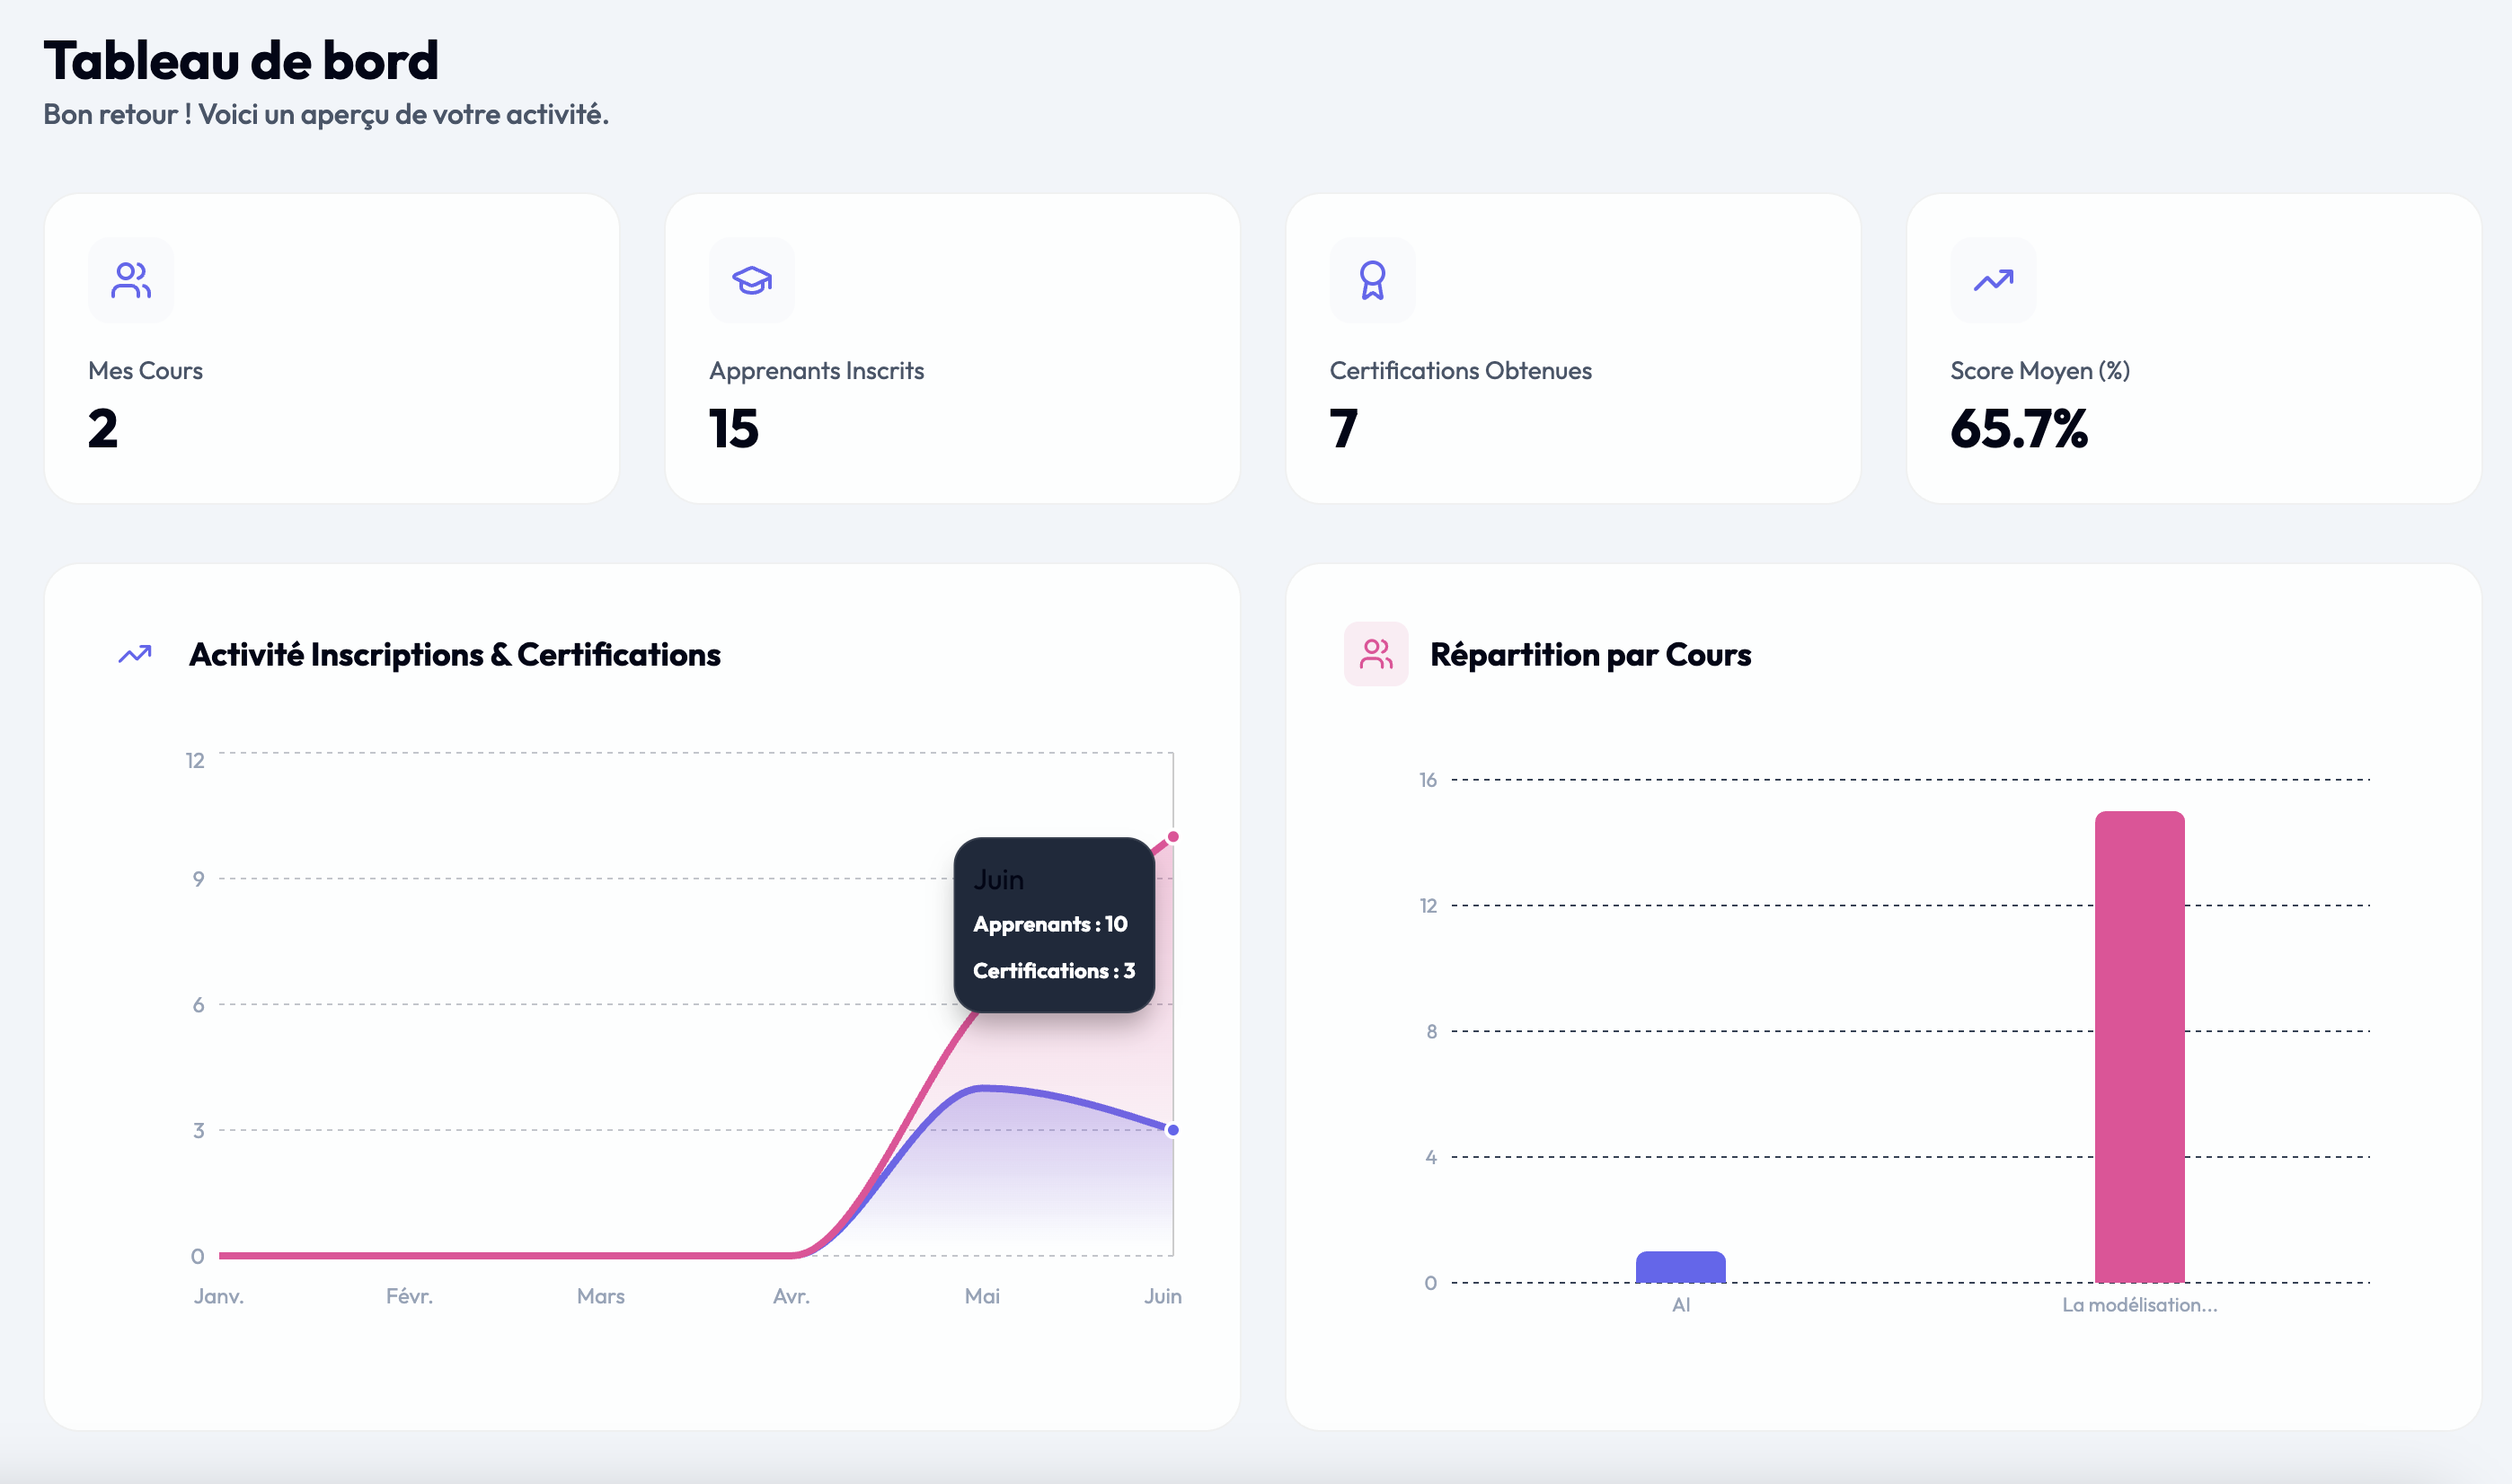
\includegraphics[width=0.98\textwidth]{figures/statistiques_test_user.png}
    \caption{Tableau de bord présentant les statistiques des tests utilisateurs (Master MSDIE).}
    \label{fig:statistiques_test_user}
\end{figure}

%%%%%%%%%%%%%%%%%%%%%%%%%%%%%%%%%%%%%%%%%%%%%%%%%%%%%%%%%%%
\section{Conclusion}
%%%%%%%%%%%%%%%%%%%%%%%%%%%%%%%%%%%%%%%%%%%%%%%%%%%%%%%%%%%
Pour clore ce chapitre, il est important de faire un bilan sur l’ensemble des décisions techniques et de réalisation qui ont été prises :

\begin{itemize}
    \item \textbf{Synthèse des choix techniques :} Les technologies, outils et méthodologies adoptés, tels que \textbf{Java (Spring Boot)}, \textbf{Python (FastAPI)} et \textbf{React}, ont prouvé leur adéquation avec les besoins du projet. Ce choix technologique garantit une simplicité d'utilisation pour l'utilisateur final, des performances élevées pour les traitements IA et une grande évolutivité pour les futurs développements.
    
    \item \textbf{Retour sur l’architecture de déploiement et l’implémentation :} L’environnement de déploiement basé sur \textbf{Docker} et la structure du code organisée en microservices assurent la stabilité et la pérennité du système. Ce découpage modulaire permet de maintenir une infrastructure robuste capable de supporter des charges variables tout en facilitant les mises à jour indépendantes des services.
    
    \item \textbf{Perspectives et défis :} Lors de l’implémentation, nous avons rencontré des défis techniques liés notamment à la latence du traitement d'images en temps réel et à la gestion de la mémoire pour les services d'intelligence artificielle. Ces contraintes ont été résolues par une optimisation fine des ressources. Pour les phases ultérieures, des pistes d'amélioration comme l'optimisation des modèles de langage et l'automatisation accrue du déploiement sont à envisager.
\end{itemize}

Ce chapitre constitue ainsi un socle technique solide, garantissant que les choix de développement sont cohérents avec les objectifs du projet et prêts à être mis en œuvre lors de la phase de réalisation.

    %%%%%%%%%%%%%%%%%%%%%%%%%%%%%%%%%%%%%%%%%%%%%%%%%%%%%%%%%%%
\chapter*{Conclusion générale}
\addcontentsline{toc}{chapter}{Conclusion générale}
%%%%%%%%%%%%%%%%%%%%%%%%%%%%%%%%%%%%%%%%%%%%%%%%%%%%%%%%%%%

Le projet \textbf{Certif-fun} a abouti à la création d'un écosystème innovant alliant architecture web distribuée et intelligence artificielle pour répondre au défi de l'intégrité des certifications à distance.

\paragraph{Récapitulation des objectifs :} 
Initialement centré sur la sécurisation des évaluations, le projet a relevé le défi de l'automatisation de la surveillance. Les objectifs techniques (microservices, scalabilité) et fonctionnels (proctoring temps réel, génération de quiz) ont été validés, offrant une solution complète et opérationnelle.

\paragraph{Contributions et résultats :} 
Les réalisations majeures se résument à :
\begin{itemize}[noitemsep, topsep=1pt]
    \item \textbf{Surveillance intelligente} : Intégration de \textbf{YOLOv8} et \textbf{MediaPipe} pour un suivi autonome du regard et des objets suspects.
    \item \textbf{Pédagogie augmentée} : Génération automatique de quiz via \textbf{Ollama}, garantissant la confidentialité des données.
    \item \textbf{Agilité DevOps} : Mise en œuvre d'un pipeline \textbf{CI/CD} performant assurant des déploiements fluides.
\end{itemize}

\paragraph{Limites du travail :} 
Le système rencontre toutefois des contraintes matérielles liées au coût computationnel de l'IA sur un serveur unique. La précision reste également sensible à l'environnement de l'apprenant (éclairage, caméra), et l'authentification mériterait d'être renforcée par un contrôle biométrique continu.

\paragraph{Perspectives futures :} 
Les pistes d'évolution incluent la migration vers \textbf{Kubernetes} pour une scalabilité élastique, l'intégration de la \textbf{reconnaissance faciale continue} et le déport de l'IA vers le navigateur (\textit{Edge Computing}). L'ajout d'analyses prédictives permettrait également d'anticiper les risques de décrochage.

En conclusion, \textbf{Certif-fun} constitue un socle technologique solide, démontrant que l'IA peut devenir le garant de la crédibilité des diplômes numériques de demain.

    %%%%%%%%%%%%%%%%%%%%%%%%%%%%%%%%%%%%%%%%%%%%%%%%%%%%%%%%%%%
\chapter*{Apport du projet}
\addcontentsline{toc}{chapter}{Apport du projet}
\label{ch:apport}
%%%%%%%%%%%%%%%%%%%%%%%%%%%%%%%%%%%%%%%%%%%%%%%%%%%%%%%%%%%

Ce Projet de Fin d'Études a été un catalyseur de transformation personnelle et professionnelle, nous confrontant à la dualité entre l'idéal théorique et le pragmatisme technique du terrain.

\paragraph{Une démarche de résolution de problèmes :}
Au-delà de la technique, ce travail nous a enseigné qu'innover ne se résume pas à empiler des outils, mais à structurer une démarche scientifique. Chaque étape, de l'extraction des besoins à l'inférence des modèles d'IA, a agi comme une leçon de résilience. Nous avons appris à valider nos hypothèses par l'expérimentation constante, transformant chaque obstacle en une opportunité d'affiner notre compréhension du système.

\paragraph{Polyvalence technologique et méthodologique :}
L'acquisition de compétences a été multidimensionnelle :
\begin{itemize}[noitemsep, topsep=1pt]
    \item \textbf{Agilité (Scrum) :} L'adoption du cadre Scrum nous a appris l'importance de la livraison incrémentale et de la flexibilité face aux imprévus.
    \item \textbf{Rigueur rédactionnelle (\LaTeX) :} L'utilisation de \LaTeX a imposé une discipline de fer dans la structuration et la présentation de la documentation technique.
    \item \textbf{Architecture Microservices :} Naviguer entre Java, Python et JavaScript nous a permis de maîtriser la communication au sein d'un écosystème hétérogène.
\end{itemize}

\paragraph{Défis rencontrés et résilience :}
Le parcours a été jalonné d'embûches. Les délais stricts et les limitations de puissance de calcul ont parfois freiné nos ambitions. L'intégration de modèles \textbf{Deep Learning} gourmands sur un environnement standard a nécessité une optimisation constante pour garantir la viabilité du prototype sans sacrifier ses performances.

\paragraph{Analyse critique et perspectives :}
Avec le recul, une planification plus granulaire aurait permis de mieux anticiper les risques de latence. Pour une itération future, nous privilégierions une infrastructure Cloud optimisée GPU pour accélérer les traitements de vision. Une documentation interne plus exhaustive dès le départ aurait également facilité la maintenance.

En conclusion, ce projet a été le pont entre notre parcours académique et nos ambitions professionnelles. Il nous a doté d'une vision systémique essentielle pour notre future carrière d'ingénieur.

    
    \printbibliography[heading=bibintoc, title={References}]
    
\newpage
\thispagestyle{empty}
\begin{center}
\begin{tcolorbox}[arc=3mm,colframe=mainblue,colback=white,boxrule=0.8pt,left=10pt,right=10pt,top=12pt,bottom=12pt,width=0.93\textwidth]
\centering

\includegraphics[width=4cm]{figures/moi.png}\\[0.5cm]
{\Large\bfseries Anas Khaiy\par}
\vspace{0.3cm}
{\large\bfseries\color{mainblue}Résumé du Projet\par}
\vspace{0.5cm}
{\color{mainblue}\rule{0.55\linewidth}{0.8pt}\par}
\vspace{0.7cm}
\justifying
Le projet \textbf{Certif-fun} consiste en la conception d'une plateforme intelligente dédiée à la gestion des certifications et à la supervision sécurisée des examens à distance. L’objectif central est de restaurer la confiance dans les évaluations numériques grâce à une architecture distribuée et des capacités de surveillance automatisée en temps réel.

Les contributions majeures résident dans la mise en œuvre d’un système ergonomique permettant de détecter les comportements non autorisés tout en fluidifiant le parcours de l'apprenant. La validation du prototype a démontré des gains significatifs en termes de réactivité et de sécurité, surpassant les approches conventionnelles par une automatisation accrue des tâches de contrôle.

Ce travail a permis de renforcer des compétences avancées en ingénierie logicielle et en gestion de systèmes complexes dans un environnement exigeant. Il offre des perspectives prometteuses pour l’évolution des standards pédagogiques, notamment par l'optimisation continue de l'analyse comportementale et l'amélioration de l'ergonomie globale.

L'ensemble de ces réalisations témoigne de l'engagement à proposer une solution innovante et structurée, répondant avec précision aux problématiques de crédibilité des diplômes délivrés en ligne.

\vspace{0.8cm}
{\color{mainblue}\rule{0.65\linewidth}{0.6pt}\par}
\vspace{0.3cm}
\noindent\textbf{\color{mainblue}Mots-clés :} Certification en ligne, Proctoring automatisé, Intégrité des évaluations, Architecture microservices, Innovation pédagogique.
\end{tcolorbox}
\end{center}
\end{document}
